%%%%%%%%%%%%%%%%%%%%%%%%
%% Sample use of the infthesis class to prepare a thesis. This can be used as 
%% a template to produce your own thesis.
%%
%% The title, abstract and so on are taken from Martin Reddy's csthesis class
%% documentation.
%%
%% MEF, October 2002
%%%%%%%%%%%%%%%%%%%%%%%%

%%%%
%% Load the class. Put any options that you want here (see the documentation
%% for the list of options). The following are samples for each type of
%% thesis:
%%
%% Note: you can also specify any of the following options:
%%  logo: put a University of Edinburgh logo onto the title page
%%  frontabs: put the abstract onto the title page
%%  deptreport: produce a title page that fits into a Computer Science
%%      departmental cover [not sure if this actually works]
%%  singlespacing, fullspacing, doublespacing: choose line spacing
%%  oneside, twoside: specify a one-sided or two-sided thesis
%%  10pt, 11pt, 12pt: choose a font size
%%  centrechapter, leftchapter, rightchapter: alignment of chapter headings
%%  sansheadings, normalheadings: headings and captions in sans-serif
%%      (default) or in the same font as the rest of the thesis
%%  [no]listsintoc: put list of figures/tables in table of contents (default:
%%      not)
%%  romanprepages, plainprepages: number the preliminary pages with Roman
%%      numerals (default) or consecutively with the rest of the thesis
%%  parskip: don't indent paragraphs, put a blank line between instead
%%  abbrevs: define a list of useful abbreviations (see documentation)
%%  draft: produce a single-spaced, double-sided thesis with narrow margins
%%
%% For a PhD thesis -- you must also specify a research institute:
\documentclass[phd,icsa,twoside,logo]{infthesis}
%% For an MPhil thesis -- also needs an institute
% \documentclass[mphil,ianc]{infthesis}

%% MSc by Research, which also needs an institute
% \documentclass[mscres,irr]{infthesis}

%% Taught MSc -- specify a particular degree instead. If none is specified,
%% "MSc in Informatics" is used.
% \documentclass[msc,cogsci]{infthesis}
% \documentclass[msc]{infthesis}  % for the MSc in Informatics

%% Master of Informatics (5 year degree)
% \documentclass[minf]{infthesis}

%% Undergraduate project -- specify the degree course and project type
%% separately
% \documentclass[bsc]{infthesis}
% \course{Artificial Intelligence and Psychology}
% \project{Fourth Year Project Report}

%% Put any \usepackage commands you want to use right here; the following is 
%% an example:
\usepackage{natbib}
\usepackage{relsize}
%
% Packages and Commands specific to article (see 3)
%
% These ones  are used in the guide, replace with your own.
% 
\usepackage{multicol}
\usepackage{subcaption}
%%% Customise %%%

\usepackage{xspace}
\newcommand{\Lord}{\textsc{Lord}\xspace}

\usepackage{pgfplots}
\usepgfplotslibrary{dateplot}

\usepackage{tikz}
\newcommand\tikzmark[1]{\tikz[remember picture,overlay]\node (#1) {};}
\usetikzlibrary{decorations.pathreplacing,calc,shapes,positioning}
\pgfplotsset{
    legend image with text/.style={
        legend image code/.code={%
            \node[anchor=center] at (0.3cm,0cm) {#1};
        }
    },
}

\usepgfplotslibrary{
  groupplots,
}
\definecolor{kirby}{RGB}{215,72,148}
\definecolor{kirby-light}{RGB}{242,198,221}
\definecolor{kirby-blue}{RGB}{68,102,191}
\definecolor{kirby-green}{RGB}{35,135,37}
\definecolor{kirby-dp}{RGB}{221,4,89}
\definecolor{airforceblue}{rgb}{0.36, 0.54, 0.66}
\usepackage{listings, listings-rust, listings-racket}
\usepackage{parcolumns}
\usepackage[utf8]{inputenc}
\usepackage[tt = false, type1 = true]{libertine}
\usepackage{amsmath}
% \usepackage{newtxmath}
%\usepackage{amssymb}
\usepackage[libertine]{newtxmath}
\usepackage{mathpartir}
\newcommand{\metaDef}{\mathrel{\mathop:}=}
\newcommand{\metaBound}{<\mathrel{\mathop:}}
\newcommand{\cmid}{\ \mid \ }
\newcommand{\sep}{\ , \ }
\newcommand{\Rplus}{\protect\hspace{-.1em}\protect\raisebox{.35ex}{\smaller{\smaller\textbf{+}}}}
\newcommand{\Cpp}{\mbox{C\Rplus\Rplus}\xspace}
\usepackage[font=small,skip=0pt]{caption}
\usepackage{tikz-cd}
\usepackage{graphicx}
\captionsetup[figure]{font=small,skip=0pt}
%define listing box
\lstdefinestyle{boxedlst}{
commentstyle=\color[RGB]{34,139,34}
, stringstyle=\color[rgb]{0, 0, 0.5}%
, keywordstyle=\color[RGB]{215,72,148}
, numbers=left%
, firstnumber=auto%
, numberblanklines=true%
, frame=trbL%
, numberstyle=\tiny%
, frame=leftline%
, numbersep=7pt%
, framesep=5pt%
, framerule=10pt%
, xleftmargin=15pt%
, backgroundcolor=\color[gray]{0.97}%
, rulecolor=\color[gray]{0.90}%
}
\newcommand{\mylstinline}[1]{\texttt{\footnotesize#1}}
\newcommand{\Primrose}{\textsf{Primrose}\xspace}
% \usepackage{cleveref}

\usepackage{tikz-qtree}
\tikzset{level distance = 1.5em}
\usepackage{rotating}
\newcommand{\metaDeff}{\mathrel{\mathop{::}}=}
\newcommand{\seqcomp}{\, \mathrel{\mathop;} \, }
\newcommand{\sseqcomp}{\, \mathrel{\mathop;}_s \, }
\newcommand{\lchoice}{<\mathrel{\mathop+}}
\newcommand{\slchoice}{<\mathrel{\mathop+}_s}
\newcommand{\choice}{<\mathrel{\mathop+}\mathrel{\mathop>}}
\newcommand{\schoice}{<\mathrel{\mathop+}\mathrel{\mathop>}_s}
\newcommand{\barr}{\,|\, }
\newcommand{\approximation}{\,\triangle\,}
\newcommand{\approximationdiv}{\,\mathrel{\mathop\triangle}_\infty\,}
\newcommand{\sskip}{\text{SKIP}\xspace}
\newcommand{\sabort}{\text{ABORT}\xspace}
\newcommand{\err}{\mathit{err}}
\newcommand{\dive}{\mathit{div}}
\newcommand{\one}{\text{\textit{one}\/}\xspace}
\newcommand{\ones}[1][s]{\ensuremath{\one_{#1}}}
\newcommand{\some}{\text{\textit{some}\/}\xspace}
\newcommand{\somes}[1][s]{\ensuremath{\some_{#1}}}
\newcommand{\all}{\text{\textit{all}\/}\xspace}
\newcommand{\alls}[1][s]{\ensuremath{\all_{#1}}}
\newcommand{\add}{\text{\textit{add}\/}\xspace}
\newcommand{\adds}[1][s]{\ensuremath{\add_{#1}}}
\newcommand{\atomic}{\text{\textit{atomic}}}
\newcommand{\try}{\text{\textit{try}}}
\newcommand{\tdef}{\textbf{def}}
\newcommand{\tundef}{\textbf{undef}}

\usetikzlibrary{calc,decorations.pathmorphing}
\newcounter{squig}
\newcommand\xsquigglyright[1]{%
\stepcounter{squig}%
\mathrel{\begin{tikzpicture}[baseline= {( $ (current bounding box.south) + (0,-0.5ex) $ )}]
\node[inner sep=.5ex] (\thesquig) {$\scriptstyle #1$};
\path[draw,<-,decorate,
  decoration={snake,amplitude=0.75pt,segment length=1.5mm,pre=lineto,pre length=2pt}]
    (\thesquig.south east) -- (\thesquig.south west);
\end{tikzpicture}}%
}
%%%%%%%%%%%%%%%%%%%%%%%%%%%%%%%%%%%%%%%%%%%%%%%%%%%%%%%%%%%%%%%%%%%%%%%%%%%%%%
\DeclareSymbolFont{frenchscript}{OMS}{ztmcm}{m}{n}
\DeclareMathSymbol{\Pow}{\mathord}{frenchscript}{80} % power set
%%%%%%%%%%%%%%%%%%%%%%%%%%%%%%%%%%%%%%%%%%%%%%%%%%%%%%%%%%%%%%%%%%%%%%%%%%%%%%
%%%%%%%%%%%%%%%%%%%%%%%%%%%%%%%%%%%%%%%%%%%%%%%%%%%%%%%%%%%%%%%%%%%%%%%%%%%%%

%%%%%%%%%%%%%%%%%%%%%%%%%%%%%%%%%%%%%%%%%%%%%%%%%%%%%%%%%%%%%%%%%%%%%%%%%%%%%%

%%%%%%%%%%%%%%%%%%%%%%%%%%%%%%%%%%%%%%%%%%%%%%%%%%%%%%%%%%%%%%%%%%%%%%%%%%%%%
%%%%%%%%%%% Add possessive citations, e.g. "Leroy's (1992)", taken
\usepackage{suffix}
\newcommand{\citepos}[1]{\citeauthor{#1}'s~\citeyearpar{#1}}
\WithSuffix\newcommand\citepos*[2]{\citeauthor{#1}'s #2~\citeyearpar{#1}}
\WithSuffix\newcommand\citepos-[2]{\citeauthor{#1}#2~\citeyearpar{#1}}
%%%%%%%%%%%%%%%% End of possessive citation %%%%%%%%%%%%%%%%%%%%%
%%%%%%%%%%% Misc macros by Ohad %%%%%%%%%%%%%%%%%
\newcommand\wcpo{$\omega$-cpo}
%%%%%%%%%%% end of misc macros by Ohad %%%%%%%%%%%%%%%%%
\usepackage{pifont}% http://ctan.org/pkg/pifont
\newcommand{\cmark}{\ding{51}}%
\newcommand{\xmark}{\ding{55}}%
\usepackage{csquotes}

% a pitchfork for lookup
\DeclareFontFamily{U}{FdSymbolC}{}
\DeclareFontShape{U}{FdSymbolC}{m}{n}{<-> s * FdSymbolC-Book}{}
\DeclareSymbolFont{fdarrows}{U}{FdSymbolC}{m}{n}
\DeclareMathSymbol{\pitchforkup}{\mathrel}{fdarrows}{"75}
\DeclareMathSymbol{\downspoon}{\mathrel}{fdarrows}{'153}
\DeclareMathSymbol{\upspoon}{\mathrel}{fdarrows}{'151}

% a box arrow for update
\DeclareFontFamily{U}{txsyc}{}
\DeclareFontShape{U}{txsyc}{m}{n}{<-> s * txsyc}{}
\DeclareSymbolFont{txarrows}{U}{txsyc}{m}{n}
\DeclareMathSymbol{\boxRight}{\mathrel}{txarrows}{"88}

\usepackage{wrapfig}

\newcommand{\V}{\mathcal{V}}
\newcommand{\plat}[1]{\raisebox{0pt}[0pt][0pt]{#1}}     % no vertical space

% typesetting theorems
\newtheorem{theorem}{Theorem}[section]
\newtheorem{lemma}[theorem]{Lemma}
\newtheorem{definition}{Definition}[section]
%%

%% cute stuff
\usepackage{pgfornament}
\newcommand{\framesize}{\textwidth}
%%

%% Information about the title, etc.
\title{Necronomicon: Studies Concerning the Meaning of Computer Programs}
\author{Xueying Qin}

%% If the year of submission is not the current year, uncomment this line and 
%% specify it here:
% \submityear{1785}

%% Optionally, specify the graduation month and year:
% \graduationdate{February 1786}

%% Specify the abstract here.
\abstract{%
    This doctoral thesis will present the results of my work into the
    reanimation of lifeless human tissues.
}

%% Now we start with the actual document.
\begin{document}

%% First, the preliminary pages
\begin{preliminary}

%% This creates the title page
\maketitle

%% Acknowledgements
\begin{acknowledgements}
I thank myself for not being able to end my life.
\end{acknowledgements}

%% Next we need to have the declaration.
\standarddeclaration

%% Finally, a dedication (this is optional -- uncomment the following line if
%% you want one).
% \dedication{To my mummy.}

%% Create the table of contents
\tableofcontents

%% If you want a list of figures or tables, uncomment the appropriate line(s)
% \listoffigures
% \listoftables

\end{preliminary}

%%%%%%%%
%% Include your chapter files here. See the sample chapter file for the basic
%% format.

\chapter{Climbing Tower of Babel}
\label{chap1}
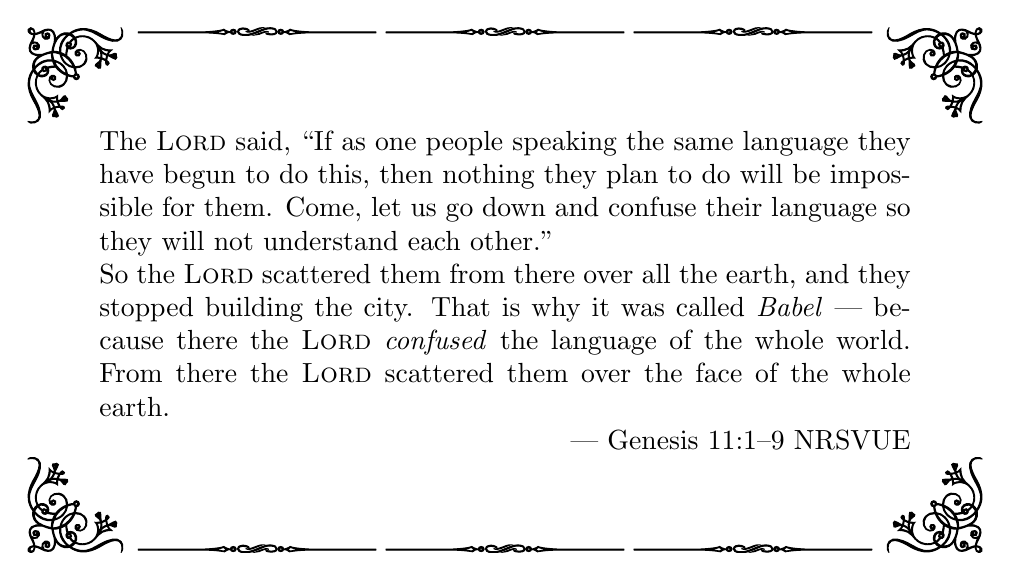
\begin{tikzpicture}[color=black,
                   transform shape,
                   every node/.style={inner sep=0pt}]
\node[minimum width=\framesize, minimum height=0.55 *\framesize, fill=white](vecbox){};
\node[anchor=north west] at (vecbox.north west){% 
\pgfornament[width=0.1*\framesize]{61}};
\node[anchor=north east] at (vecbox.north east){% 
\pgfornament[width=0.1*\framesize,symmetry=v]{61}};
\node[anchor=south west] at (vecbox.south west){% 
\pgfornament[width=0.1*\framesize,symmetry=h]{61}};
\node[anchor=south east] at (vecbox.south east){% 
\pgfornament[width=0.1*\framesize,symmetry=c]{61}};
\node[anchor=north] at (vecbox.north){% 
\pgfornament[width=0.25*\framesize]{88}
\pgfornament[width=0.25*\framesize]{88}
\pgfornament[width=0.25*\framesize]{88}
};

\node[anchor=south] at (vecbox.south){% 
\pgfornament[width=0.25*\framesize]{88}
\pgfornament[width=0.25*\framesize]{88}
\pgfornament[width=0.25*\framesize]{88}
};
\node[text width=0.85\framesize, align=justify] at (vecbox.center){%
The \Lord said, ``If as one people speaking the same language they have begun to do this, then nothing they plan to do will be impossible for them. Come, let us go down and confuse their language so they will not understand each other."
\\
So the \Lord scattered them from there over all the earth, and they stopped building the city. That is why it was called \emph{Babel} --- because there the \Lord \emph{confused} the language of the whole world. From there the \Lord scattered them over the face of the whole earth.\\
\rightline{--- Genesis 11:1–9 NRSVUE}};
\end{tikzpicture}
% Humans are divided into different linguistic groups, therefore, they are unable to understand each other. Yet, there are people trying to understand others, from a linguistic perspective, a cognitive perspective, a psychological perspective, a social perspective etc. Naturally, the gap between humans and machines is wider than the gap between different human linguistic groups. Again, there are people studying different layers of machine languages and the process of translating (i.e., compilation and interpretation) human languages into machine codes. 
% THE MYTHOLOGY %
\lettrine{H}{umans} are divided into different linguistic groups, therefore, they are unable to understand each other. That said, ``meaning" is encoded into different conceptual schemes in different languages; without accurate translations, it is ultimately difficult for people who speak different languages to communicate with each others. In addition, due to the nature of natural language being ambiguous, it is hard to accurately reason about what others \emph{really mean} even under the context of a same language.

% PHLOSOPHY %
Over the decades, there has been various studies concerning the \emph{meaning} of languages. The term \emph{semantics} is used to refer to the studies of linguistic meaning~\citep{katz1972, palmer1981semantics}. From a philosophical perspective, there are different theories of meaning. \citet{lewis1970} describes two topics of the studies of meaning. Corresponding to the first observation from the mythology --- ``meaning is encoded into different conceptual schemes in different languages" --- the first topic concerning the meaning of languages is to understand the psychological and sociological facts that a person or a group of people give certain meanings to the symbols in their languages~\citep{lewis1970}. One kind of approaches are \emph{ideational theories}~\citep{ChapmanRoutledge+2009+84+85}, which examines the meaning in terms of and as an output of people's mental representations~\citep{Stich1994-STIMR}. A different point of view is initiated by \citet{Kripke1980-KRINAN}, who argues against the idea of proper name being synonymous with definite descriptions, while proposing that names are associated with their referents through a causal chain of reference. Such a \emph{causal theory} further suggests that the meaning of an expression instead of being inherited from mental states, is determined by the causal connections that the expression has with the objects or concepts that it~refers~to. 

Corresponding to the second observation --- ``it is hard to accurately reason about what others really mean even under the context of a same language" --- the second topic is to accurately examine and analyse the meaning of an expression (i.e., a word or a sentence) in a given language~\citep{lewis1970}. Specifically, \citet{frege1892} introduces a \emph{theory of reference}, suggesting that meaning of a expression involves both its reference to an object, which is a proper name that contributes to the truth value of a sentence, and its sense, which is how the object is presented. Using the example sentence ``the present King of France is bald", \emph{Russell's theory of description}~\citep{russell1904} argues that Frege's notion of sense and reference is not sufficient for analysing an expression which has sense but no reference, while introducing a rigorous analytic method for problematic propositions, concerning denoting phrases, making use of the machinery of first-order logic featuring propositional functions. Following \citepos{tarski1944} truth definition of a sentence, \citet{davidson1967} proposes an approach with the core idea that meaning should be understood based on a \emph{formal theory of truth}. There are also \emph{semantic internalism} theories~\citep{Mcgilvray1998, Chomsky2000, pietroski2017semantic} that instead of giving truth value to expressions, view the meaning of an expression as what is used for building a particular mental representation. Taking a holistic approach to analyse the meaning of expressions, \emph{inferential semantics} theories~\citep{Brandom2000} argue against the idea using establish truth conditions to further analyse good and bad inferences, instead, suggest to first study the distinction between good and bad inferences, which provides the basis for understanding truth conditions. Hence the meaning of an expression is studied in relation to other~expressions. 
% There are topic knowledge representation, semantic parsing
\begin{center}
\vspace{-0.7em}
\pgfornament[width=0.08*\framesize]{11}
\pgfornament[width=0.08*\framesize]{80}
\pgfornament[width=0.08*\framesize]{14}
\vspace{-0.3em}
\end{center}

% LINGUISTICS %
Linguists tend to adopt less abstract approaches to analyse the meaning of languages. There are also many different topics within linguistic studies of semantics.

One important field of linguistic semantics is \emph{lexical semantics}, which concerns the meaning of words~\citep{palmer1981semantics, PUSTEJOVSKY200698, LexicalSemantics}, including topics such as the \emph{semantic structure} of words like ambiguity and polysemy as well as the semantic relations between words such as metaphor and metonymy, \emph{lexical fields} (alternatively \emph{semantic fields}) which has been initially introduced by \citet{trier1931deutsche} studying the meaning of words according to their relationship to other words of which the meanings are interdependent~\citep{palmer1981semantics, jackson2000words}, and \emph{lexical relations} which studies the structural relation between words like synonymy and antonymy~\citep{LexicalSemantics}.

Another widely explored field of linguistic semantics is \emph{structural semantics}, or more general, \emph{structural linguistics}, which is inspired by \citepos{Saussure1916} semiotic analysis centring linguistic signs, attempting to analyse a language as a structured system of interrelated elements. In particular, the aforementioned topics like semantic fields and lexical relations along with other semantic relation between words have been taken from the lexical studies and further developed into a structured basis for the analysis or words' meaning~\citep{LexicalSemantics}. Such an influential approach has later been adapted into the studies of generative grammars and their formalism~\citep{Katz1963-KATTSO-3, Chomsky1975-CHOTLS}.

\emph{Cognitive semantics} is a major part of cognitive linguistics, which is an important linguistic field has been explored through decades by \citet{Johnson1987-JOHTBI}, \citet{alma9923109163502466}, \citet{alma993245163502466}, \citet{fauconnier1998}. taking an alternative approach from the structural linguistics, it studies the meaning of languages under the context of human cognition, specifically, viewing semantics as a conceptual organisation of languages~\citep{10.7551/mitpress/6847.001.0001, Croft_Cruse_2004}.

Perhaps along with the emerging natural language processing technology such as ChatGPT, the field \emph{computational linguistics}, concerning modelling natural languages as computational models, has now become one of most popuar areas. \emph{Computational semantics}, as an important study within the scope of the computational linguistics, enable automatic analysis of sentences' meaning via machines~\citep{mitkov2022}. Base on the aforementioned fields such as lexical semantics and structural semantics as well as formal semantics like Montague semantics~\citep{Montague1970-MONEAA-2} which will be later discussed, the main focus of this field is the \emph{representation} of meaning, where the meaning of the languages are represented via some formal structures, for instance, logic forms including propositional logic~\citep{boole1854investigation} and first order predicate logic~\citep{Frege1879-FREBAF-2}, discourse representation structure studies in discourse representation theory~\citep{Kamp1993-KAMFDT}, and event structures~\citep{PUSTEJOVSKY199147}, tense logic~\citep{Prior1955-PRITAM, Kamp1968-KAMTLA} as well as the temporal anaphora that provides representations of events and time in sentences~\citep{partee1884, hinrichs1986}. Semantic parsing is the technique being studied to transform sentences into these semantic representations, while semantic analysis and semantic inference are perform on these semantic representations for automatically processing the meaning of sentences. 

Originated from philosophical view, especially the logic of languages, linguistic formal semantics focusing on analysing the truth condition aspect of meaning with frameworks concerning compositionality, specifically, a formal analysis of the semantics of some language is achieve base on a syntactic formalism of a language~\citep{alma999704883502466}. Although obviously the study of linguistic formal semantics does not intend to explore all features of the semantics of the natural languages, it explores ways for precise modelling of the syntax as well as analysis of semantics of sentences. An important work within such an field is categorial grammar, of which \citepos{Adj35} development provides a formal syntactic approach for analysing higher-order logic. Such an approach has been later adapted for analysing natural languages, such as Lambek calculus~\citep{Lambek1958-LAMTMO-5}. Montague semantics, which is a model-theoretical approach, providing a relation between syntax and semantics~\citep{Montague1970-MONEAA-2}. It analyses a subset of English, taking the form of Montague grammar, with lambda calculus, higher-order functions, and type theory. Combintorial categorial grammar~\citep{steedman2001, steedman2011combinatory} further provides formalism of categorial grammar with combintorial logic, which shares the same level of expressiveness as lambda calculus.
\begin{center}
\vspace{-0.7em}
\pgfornament[width=0.08*\framesize]{11}
\pgfornament[width=0.08*\framesize]{80}
\pgfornament[width=0.08*\framesize]{14}
\vspace{-0.3em}
\end{center}

% From Natural Languages to Programming Languages
As we have discussed in the previous paragraphs, within the scope of the linguistic formal studies concerning structured and systematic analysis of the meaning of languages including computational and formal semantics, various formal systems and logic frameworks such as lambda calculus, first order logic, modal logic, combintorial logic, category theory etc. are used in modelling formal syntactical representations of natural languages to enable precise analysis of the semanticsas well as to facilitate machines to understand and generate meaningful structured sentences. Perhaps not surprisingly, these formal systems and logic components also form an important foundation for the design and analysis of \emph{programming languages}.

% COMPUTER SCIENCE %
% Naturally, the gap between humans and computers is even larger than the gap between different human linguistic groups. 
Programming languages are created by human, serving as an interface for human to communicate and interact with computers. Since humans tend to encode and express information in terms of structured phrases and sentences, like natural languages, programming languages are designed to have grammar and syntax for human to convey their intentions to computers taking the form \emph{computer programs}. While computers execute binary code containing zeros and ones, the communication processes between humans and computers are facilitated by compilers, which are responsible for translating information encoded by humans taking the form of computer programs into executable machine code. The study of programming languages explores different approaches for effectively expressing better abstractions in various application domains, facilitating accurate and efficient compilation process, and providing better frameworks for humans to understand and reason about the behaviours of computers' executions of programs.

% Before stepping into the clich\'e of introducing the formal semantics of programming languages, a question is necessary to be asked. We keep saying that the study of semantics is the study of the meaning of languages, however, \emph{what is ``meaning"?} Within the scope of programming language studies, it is: 0) how we \emph{model} and \emph{understand} programs; 1) how we \emph{communicate} what we want computers to do in terms of programs with computers; 2) how we \emph{reason about} the behaviours of programs.

The study of formal semantics of programming languages has been around for decades and three main forms of formal semantics have been used serving as a foundation for understanding and reasoning about computer programs~\citep{10.5555/151145, citeulike:105547}. Specifically, \emph{operational semantics} provides meanings to programs by modelling how computations get executed. In particular, \emph{small-step operational semantics} focuses on the incremental reduction of expressions or states, providing a detailed and precise understanding of program behaviours, while \emph{big-step operational semantics} describes the execution of programs in terms of its overall behaviours or outcomes rather than its individual intermediate execution steps. Operational semantics is particularly useful for the implementation of a programming language. \emph{Denotational semantics} gives meanings to programs by modelling the result of computations as mathematical objects. It abstract away the details of the execution of programs and gives an elegant mathematical model presenting the core concepts of a programming language. Instead of modelling how computations get executed or what are produced by executions of computations, \emph{axiomatic semantics} provides meanings to programs by specifying properties satisfied by the results produced by executions of computations. In practice, it is particularly useful for building a proof system for reasoning about the execution of programs.

In my three-year short research journey, my fundamental motivations are to gain precise understanding of humans' mental models of computer programs and to improve the design of programming languages in order to allow humans to effectively communicate with computers. Corresponding to the foundational programming languages semantics study, I intend to explore ways to design better abstractions to \emph{model} and \emph{understand} programs in order to allow programmers to effectively \emph{communicate} what they want computers to do in terms of programs and precise formal frameworks allowing us to \emph{reason about} the behaviours of complicated realistic programs.
Till the end of this journey, I have asked three conceptual questions, and conducted three studies concerning the meaning of computer programs, utilising modelling and reasoning techniques presented in the existing studies of formal semantics of programming languages.

% Hence, it is important to study the \emph{meaning} of programs expressed using these languages, i.e., the semantics of programming languages.
% As a computer scientist who is specialised in the study of programming languages, through this three-year short research journey, my fundamental motivations are to gain formal and precise understanding of humans' conceptual scheme of computer programs and to improve the design of programming languages in order to allow humans to effectively communicate with computers. To understand programming languages and communicate with machines via these languages, it is important to study the \emph{meaning} of programs expressed using these languages, i.e., the semantics of programming languages.

% Due to my nature of stupidity, I am in no position to invent yet another way to study the meaning of programming languages. Instead, in my three useless and insignificant projects, I merely ask three conceptual questions and attempt to answer them via studying and making use of existing formal semantics models.

\begin{center}
\vspace{-0.7em}
\pgfornament[width=0.08*\framesize]{11}
\pgfornament[width=0.08*\framesize]{80}
\pgfornament[width=0.08*\framesize]{14}
\vspace{-0.3em}
\end{center}

The first conceptual question asked is: 
How to design a better abstraction mechanism that allows programmers to effectively express \emph{what} they want a computer to do via some declarative yet accurate \emph{specifications} instead of \emph{how} a computer should accomplish a task via some concrete \emph{implementations}?
% in order to achieve better automation?

\emph{Formal specification} is a rigorous and systematic approach to defining the behaviour, structure, and properties of a system with a specification language of which the syntax and semantics are formally defined such as Z, Alloy, and VDM or logic like first-order logic, linear temporal logic (LTL), and computational tree logic (CTL). It involves describing a system's functionality, constraints, and requirements using precise and unambiguous terms that can be understood both by humans and potentially processed by automated tools for verification and validation.

The major application of formal specifications is to verify and validate software systems, ensure certain properties are satisfied. In addition, formal specifications of a system also form a clear and precise documentation of the system's requirements, which facilitate communication amongst developers and maintainers of the system.

We make use yet another usage of formal specifications to address this conceptual question, which is \emph{abstraction}. They allow developers to focus on the high-level requirements of instead of detailed implementations of a system. Such an abstraction not only facilitates managing the complexity in software development but also opens up opportunities in achieving better automation and optimisation in the process of implementing a software system. In the first project, we studied container types in programming languages and their properties, focusing on decoratively describing the properties of container types using formal specifications rather than having these properties concretely implemented for the container types.
% To address this question, a topic has been taken as an instance to study, which is container types in programming languages and their properties. 

Container data types are ubiquitous in computer programming, enabling developers to efficiently store and process collections of data with an easy-to-use programming interface.
Many programming languages offer a variety of container implementations in their standard libraries based on data structures offering different capabilities and performance characteristics.
However, choosing the \emph{best} container for an application is not always straightforward, as performance characteristics can change drastically in different scenarios, and as real-world performance is not always correlated to theoretical complexity. Based on this observation, we bring up a research question: How to design a notion of container that truly allows to separate its interface and usage from the implementation and to infer the implementation from its interface and usage?

This question is answered by the project --- \emph{\Primrose{}: Selecting Container Data Types by Their Properties.}
In this project, we present \Primrose{}, a language-agnostic tool for selecting the best performing valid container implementation from a set of container data types that satisfy \emph{properties} given by application developers.
\Primrose{} automatically selects the set of valid container implementations for which the \emph{library specifications}, written by the developers of container libraries, satisfies the specified properties.
Finally, \Primrose{} ranks the valid library implementations based on their runtime performance.
With \Primrose{}, application developers can specify the expected behaviour of a container as a type refinement with \emph{semantic properties}, e.g., if the container should only contain unique values (such as a \lstinline{set}) or should satisfy the LIFO property of a \lstinline{stack}.
Semantic properties nicely complement \emph{syntactic properties} (i.e., traits, interfaces, or type classes), together allowing developers to specify a container's programming \emph{interface} and \emph{behaviour} without committing to a concrete implementation.
We present our prototype implementation of \Primrose{} that preprocesses annotated Rust code, selects valid container implementations and ranks them on their performance. The design of \Primrose{} is, however, language-agnostic, and is easy to integrate into other programming languages that support container data types and traits, interfaces, or type classes. Our implementation encodes properties and library specifications into verification conditions in Rosette, an interface for SMT solvers, which determines the set of valid container implementations. We evaluate \Primrose{} by specifying several container implementations, and measuring the time taken to select valid implementations for various combinations of properties with the solver. We automatically validate that container implementations conform to their library specifications via property-based testing.
This work provides a novel approach to bring abstract modelling and specification of container types directly into the programmer's workflow.
Instead of selecting concrete container implementations, application programmers can now work on the level of specification, merely stating the behaviours they require from their container types, and the best implementation can be selected automatically. In chapter~\ref{chap2}, we discuss this project in detail.

Back to the conceptual understanding of the relationship between specifications and implementations, in this small study, we demonstrated that property specifications and library specifications describing \emph{what} properties, especially properties giving an account of functional requirements, a container type and its operations should satisfy, which are separated from concrete container implementations describing \emph{how} properties are satisfied. Such separation of concerns enables automation and optimisation for application developers to use a container data type in their programs.

\begin{center}
\vspace{-0.7em}
\pgfornament[width=0.08*\framesize]{11}
\pgfornament[width=0.08*\framesize]{80}
\pgfornament[width=0.08*\framesize]{14}
\vspace{-0.3em}
\end{center}

The second conceptual question asked is: How to intuitively understand \emph{distributed programs} using the same conceptual model as \emph{monolithic programs}?
% How to get a intuitive understanding of distributed programs in order to simplify the process of migrating monolithic programs into distributed setting?

A monolithic architecture is a common software architecture, which features a single unit to be deployed and a single database to be connected to~\citep{Taylor09}. Despite of being inflexible and less scalable, a monolithic architecture is easy to implement, deploy, and test, especially for the development of a light-weight service. 

To address this question, a topic has been looked into, which is designing a remote procedural call library for Rust, allowing monolithic programs to be migrated into a distributed setting without massive re-coding, in the meanwhile extends Rust's memory safety guarantees into the distributed setting.

In distributed computing, a remote procedure call (RPC) allows a method invocation to be executed on another computer on a shared network. Such a remote method invocation has the same coding as a local method invocation, without the programmer explicitly encoding the details for the remote interaction. It is hard to support \emph{location transparency}, i.e., in existing RPC frameworks such as Java RMI and Rust tarpc, remote method invocations do not have \emph{the same semantics} as local method invocations. In addition, \emph{memory management} is hard in a distributed setting, for instance, distributed garbage collection is complicated.

To address these issues, we design a \emph{universal method invocation} (UMI) library in Rust supporting location transparency. With the UMI library, syntactically, a distributed program is written (almost) the same as a monolithic program; semantically, a distributed program preserves the semantics of a monolithic program. We choose Rust as a the target language for the UMI framework to utilise Rust's memory safety guarantees. Rust is high-level system programming language which \emph{guarantees memory safety} and \emph{prevents data races} by its \emph{ownership and borrow checking system} for memory management and tracking object lifetime of all references in a program during compilation. Since Rust has semantics that guarantees memory safety, we can extend such guarantees to the distributed computing setting, allowing our UMI framework to provide safe remote method invocations.

We provide a usable \emph{Rust implementation} of the UMI framework and formalise the \emph{small-step operational semantics} for a core calculus of monolithic and distributed Rust programs. In addition, we prove a \emph{location transparency theorem}: With the UMI framework, when a monolithic program is deployed to multiple nodes, its semantics is preserved.
This project is discussed in detail in chapter~\ref{chap3}.

\begin{center}
\vspace{-0.7em}
\pgfornament[width=0.08*\framesize]{11}
\pgfornament[width=0.08*\framesize]{80}
\pgfornament[width=0.08*\framesize]{14}
\vspace{-0.3em}
\end{center}

The third conceptual question asked is: 
How do we characterise the relationship between the \emph{syntax} and \emph{semantics} of programming languages?
% How to gain a formal understanding of and reason about a programming language that performs syntactic transformation? 

I am certainly not the first person asking such a question. In fact, in the world of linguistic studies, the ``linguistics wars"~\citep{alma993219653502466} happened in 60s and 70s were a academic dispute on the relationship between the syntax and semantics of natural languages. Dating back to the 50s, by presenting the sentence ``Colourless green ideas sleep furiously", which is grammatically correct but nonsensical, \citet{Chomsky+1957}
argues that the syntax of a language being independent from the semantics. However, some structural linguists emphasise that the analysis of language structure and meaning should be within a synchronic framework.

In programming languages studies, it is generally agreed that the syntax, which represents the form of programs, organises the symbols and defines the programs' structure without giving the meaning to the programs. After defining the syntax, the semantics, which is the meaning, can then be assigned to syntactic valid programs, by describing the execution of programs.

While the syntax and semantics concern different aspects of the design of programming languages, they are not completely independent. In the two previous studies, we have already discussed designs concerning syntactic properties of collections of data and minimising the changes in syntax while changing the architecture of programs. There are some perhaps conceptually important observations of the design of the syntactic contracts. Firstly, although comparing to modelling semantic properties and reasoning about the semantic preservation, these syntactic constructs seems to be too straightforward to discuss in detail and it is not straightforward to evaluate how ``well" they have been designed, they are still very important serving as an abstraction that allows and facilitates programmers to convey the intend semantics of programs. In \Primrose{}, we have seen that some semantic properties like LIFO depend on the syntactic properties, giving a characterisation of a container by stating the behaviours of specific operations given by syntactic properties. In the design of the UMI framework, the syntax serves as the abstraction for location transparency, where the location of resources is abstracted away from how programmers interact with them, while the semantics gives meaning to such an abstraction utilising which we are able to reason about that resources are properly used and managed independent from where they are stored.

In the third project, we studied the syntax and semantics of programming languages from yet another perspective, via the rewriting.
Rewriting is a versatile and powerful technique used in many domains including symbolic computation, theorem proving, programming language semantics, and compiler optimisation.
While being practically useful, rewriting is also conceptually intriguing. In a rewriting system, syntactic transformations is used to systematically encode the semantics of the reduction, simplification and evaluation of expressions. Since these syntactic transformation steps are composible, valid composition of valid syntactic transformation steps form a meaningful program, the process of composing syntactic transformation steps together has its own semantics to be examined. 

In practice, \emph{strategic rewriting} is a systematic technique that allows programmers to control the application of rewrite rules by composing individual rewrite rules into complex rewrite strategies. These strategies have concise and intuitive syntactic constructs and simply serve as compositions of syntactic transformations but are semantically complex, as they may be nondeterministic, they may raise errors that trigger backtracking, and they may not terminate.
% System S, which is a core calculus of strategic rewriting languages like Stratego, Elevate, and Strafunski, as the subject to study. We have developed denotational semantics, big-step operational semantics, and axiomatic semantics (i.e., the weakest precondition calculus) for System S in order to formally understand and reason about such a family of strategic rewriting languages.
% Rewriting is a versatile and powerful technique used in many domains.
% \emph{Strategic rewriting} allows programmers to control the application of rewrite rules by composing individual rewrite rules into complex rewrite strategies. These strategies are semantically complex, as they may be nondeterministic, they may raise errors that trigger backtracking, and they may not terminate.
Given such semantic complexity, it is necessary to establish a formal understanding of rewrite strategies and to enable reasoning about them in order to answer questions such as:
How do we characterise errors and divergence in a strategic rewriting system?
How do we understand and model nondeterminism in the executions of strategies?
How do we know that a rewrite strategy terminates?
How do we know that a rewrite strategy does not fail because we compose two incompatible rewrites?
How do we know that a desired property holds after applying a rewrite strategy?

These questions are answered by the project --- \emph{Shoggoth: A Formal Foundation for Strategic Rewriting}. It provides a semantic foundation for understanding, analysing and reasoning about strategic rewriting that is capable of answering these questions.
We provide a denotational semantics of System S, which is a core calculus of strategic rewriting languages like Stratego~\citep{DBLP:conf/icfp/VisserBT98,10.1007/3-540-45127-7_27}, Elevate~\citep{DBLP:journals/cacm/HagedornLKQGS23,DBLP:journals/pacmpl/HagedornLKQGS20}, and Strafunski~\citep{DBLP:conf/rule/LammelV02}, and prove its equivalence to our big-step operational semantics, which extends existing work by explicitly accounting for divergence.
We further define a \emph{location-based weakest precondition calculus}, which can be seen as an axiomatic semantics of System S~\cite{VISSER1998422}, to enable formal reasoning about rewriting strategies, and we prove this calculus sound with respect to the denotational semantics.
We show how this calculus can be used in practice to reason about properties of rewriting strategies, including termination, that they are well-composed, and that desired postconditions hold.
The semantics and calculus are formalised in Isabelle/HOL and all proofs are mechanised. This project is discussed in detail in chapter~\ref{chap4}.

Back to the relationship of syntax and semantics of programming languages, in this small study, the syntax and semantics are interdependent since we have observed that the transformations of the syntax of expressions encode the meaning for the evaluation of these expressions, and we can characterise and reason about the executions of compositions of these syntactic transformations by assigning to and analysing of the semantics of them. Such an observation, aside of the practical usefulness of the framework Shoggoth we build enabling formal understanding and reasoning of strategic rewriting languages, is conceptually intriguing as a perspective of the study of the syntax and semantics in the design of programming languages.

% This thesis contains three studies which explore different aspects of modelling and reasoning about programming languages:
% \begin{itemize}
%     \item The first study is designing property-based container types that allow application programmers to specify their desired properties of a container, enabling a ``best-performing" implementation to be selected from a container library accordingly. (Chapter~\ref{chap2})
%     \item The second study is the design and implementation of a remote procedural call library in Rust. (Chapter~\ref{chap3})
%     \item The third study contains the formal semantics of a strategy rewriting language: System S as well as, a weakest precondition calculus for reasoning about strategic rewriting. (Chapter~\ref{chap4})
% \end{itemize}

\chapter{Specifications, All Too Specific}
\label{chap2}
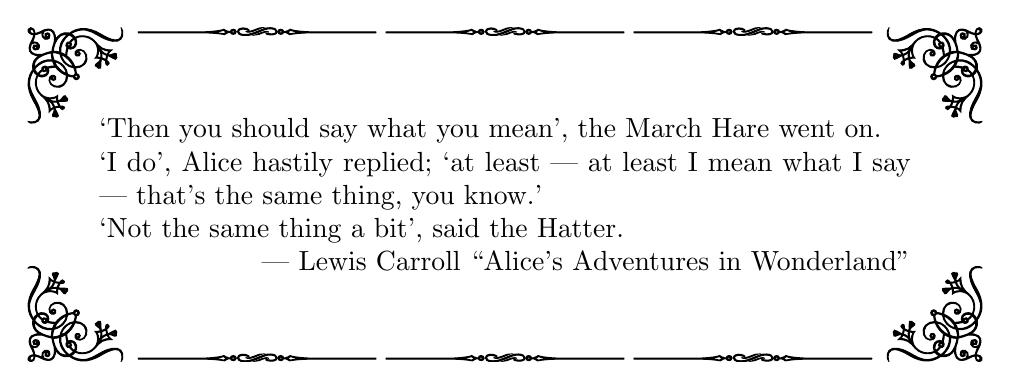
\begin{tikzpicture}[color=black,
                   transform shape,
                   every node/.style={inner sep=0pt}]
% \node[minimum size=\framesize,fill=white](vecbox){};
% \node[text width=\framesize,align=center](Text){%
%     `Then you should encode what you mean', the March Hare went on.
% \\
% `I do', Programmer hastily replied; `at least --- at least I mean what I encode --- that's the same thing, you know.'
% \\
% `Not the same thing a bit', said the Hatter.};
\node[minimum width=\framesize, minimum height=0.35 *\framesize, fill=white](vecbox){};
\node[anchor=north west] at (vecbox.north west){% 
\pgfornament[width=0.1*\framesize]{61}};
\node[anchor=north east] at (vecbox.north east){% 
\pgfornament[width=0.1*\framesize,symmetry=v]{61}};
\node[anchor=south west] at (vecbox.south west){% 
\pgfornament[width=0.1*\framesize,symmetry=h]{61}};
\node[anchor=south east] at (vecbox.south east){% 
\pgfornament[width=0.1*\framesize,symmetry=c]{61}};
\node[anchor=north] at (vecbox.north){% 
\pgfornament[width=0.25*\framesize]{88}
% \pgfornament[width=0.1*\framesize]{15}
% \pgfornament[width=0.1*\framesize]{16}
\pgfornament[width=0.25*\framesize]{88}
\pgfornament[width=0.25*\framesize]{88}
};

\node[anchor=south] at (vecbox.south){% 
% \pgfornament[width=0.25*\framesize]{88}
% \pgfornament[width=0.1*\framesize,symmetry=h]{15}
\pgfornament[width=0.25*\framesize]{88}
\pgfornament[width=0.25*\framesize]{88}
\pgfornament[width=0.25*\framesize]{88}
% \pgfornament[width=0.1*\framesize,symmetry=h]{16}
% \pgfornament[width=0.25*\framesize]{88}
};
% \node[anchor=south] at (vecbox.south){% 
% \pgfornament[width=0.6*\framesize]{46}};
% \node[anchor=north,rotate=90] at (vecbox.west){% 
% \pgfornament[width=0.6*\framesize,symmetry=h]{46}};
% \node[anchor=north,rotate=-90] at (vecbox.east){% 
% \pgfornament[width=0.6*\framesize,symmetry=h]{46}};
\node[text width=0.85\framesize,align=justify] at (vecbox.center){%
% `Then you should \emph{encode} what you mean', the March Hare went on.
% \\
% `I do', \emph{Programmer} hastily replied; `at least --- at least I mean what I \emph{encode} --- that's the same thing, you know.'
% \\
% `Not the same thing a bit', said the Hatter.\\
% \rightline{--- \emph{Altered} Alice's Adventures in Wonderland}};
% \node[text width=0.85\framesize,align=right] at (vecbox.south){%
%    --- \emph{Altered} Alice's Adventures in Wonderland};
`Then you should say what you mean', the March Hare went on.
\\
`I do', Alice hastily replied; `at least --- at least I mean what I say --- that's the same thing, you know.'
\\
`Not the same thing a bit', said the Hatter.\\
\rightline{--- Lewis Carroll ``Alice's Adventures in Wonderland"}};
\end{tikzpicture}
\section{Prologue}
\label{chap2:prologue}
People often try to \emph{say} what they \emph{mean}, however, there is always a gap between what they say and what they really mean --- \emph{they do not mean what they say.} Likewise, programmers often try to \emph{encode} what they \emph{meant for} a computer to do, however, there is always a gap between what they encode and what they really want a computer to execute --- \emph{they do not mean what they encode.}

One observation is that in an implementation of an application, what an application developer encode tends to be ``all too specific" comparing to what they have modelled in mind.
% One issue we intend to look into in this project is that encoding of container types in an application being ``all too specific". 
Take a container type example which is illustrated in later sections, when an application developer wants to use a \emph{unique container} in an application, the application developer \emph{means} that the container does not contain any duplicated elements. However, the application developer often has to \emph{encode} such a required container as a tree, a hash table, a list without duplicated element etc. By choosing a concrete encoding, application developers no longer just expresses what they mean, but additionally committing to certain performance characteristics or memory consumption which may not be desirable.

Hence, we would like to look into the designing a programming framework, facilitating application developers to better express what they meant for a computer to execute via writing declarative specifications instead of encoding concrete and fixed implementations. 
We believe that such a framework would also enable better automation and optimisation: It gives opportunities to a tool such as a compiler to select or generate a best performing implementation according to the specification provided by an application developer.

% To address this issue, we propose to design a framework, to allow application programmers to better express what they mean: What properties a container should have, instead of how these properties are implemented.

\section{Introduction}
\label{chap2:introduction}
Container data types, such as sets, lists, and trees, represent collections of data ubiquitous in everyday programming~\citep{DBLP:books/daglib/0023376}. Virtually all programming languages provide a variety of container implementations in their standard libraries.

Much work has been done to design better abstractions, improve performance and verify correctness for container data types.
However, a crucial problem for application developers using containers still exists:
when choosing a container data type, application developers are forced to select a concrete implementation that comes with certain theoretical complexity and practical performance tradeoffs.

% For example, let us consider a situation where an application developer would like to represent a mathematical set of elements, i.e., where each element should occur at most once in the set.
For example, consider representing a mathematical set, i.e., where each element should occur at most once.
In \Cpp, we must choose between \lstinline{std::set}, usually implemented as red-black trees~\citep{DBLP:journals/acta/Bayer72}, and \lstinline{std::unordered_set}, implemented as a hash table.
The hash-based implementation was added to the \Cpp standard in 2011, as the \Cpp standard has strict complexity requirements preventing the ordinary \lstinline{std::set} to be implemented as the (often faster) hash table.
Many blog posts and discussions~\citep{blog1,blog2,blog3,blog4,blog5} report on the performance of various \Cpp containers, showing the community's interest and the need for external guidance that the language itself does not provide.

In other languages, the situation is similar.
Rust provides two container implementations, \lstinline{HashSet} and \lstinline{BTreeSet}, expecting application developers to make an explicit choice between them.
Scala's complex collection library features abstract interfaces, such as the \lstinline{Set} trait, abstracting over many implementations such as \lstinline{HashSet} and \lstinline{TreeSet}.
But when creating an instance of \lstinline{Set}, a default \lstinline{HashSet} implementation is chosen regardless of the suitability of this implementation choice for the usage pattern of the application.

These examples demonstrate a general problem:
Application developers are forced to \emph{overspecify}, by having to select a concrete implementation, where we generally would like application developers to be shielded from low-level implementation details.
Application developers should primarily care about the \emph{abstract behaviour} of the containers in their application, and not how this is achieved.
The compiler, or a dedicated tool, should identify those containers that satisfy their functional requirements, and select the best implementation automatically.

In this paper, we propose an automated tool: \Primrose{}, which allows application developers to specify the expected behaviours and programming interfaces of containers as \emph{properties}.
\emph{Syntactic properties} specify the required programming interface of the container and are expressed as traits of the underlying programming language.
\emph{Semantic properties} specify the expected behaviour of the container and are written as logical predicates used as refinements of the container type.
\Primrose{} automatically selects the set of valid implementations for which the \emph{library specifications}, written by the library developers as pre- and post-conditions of the container operations, satisfy the specified syntactic and semantic properties using an SMT solver.
Finally, \Primrose{} ranks the valid library implementations based on 
their runtime performance.

% feels like i might be repeating something here..
To select the best container implementation, firstly, those container implementations which meet the functional requirements of the application developer must be determined, and then those valid container implementations must be evaluated based on non-functional requirements. While \Primrose{} does include functionality for ranking based on benchmarks, the focus of this paper is on the first of these two problems. There are many existing sophisticated techniques for selecting based on non-functional requirements, and they are highly complementary with \Primrose{}.

In this work, we apply verification and formal methods techniques, including refinement types, formal library specifications, and SMT solvers, in an innovative way to raise the level of abstraction for developers, freeing them from the burden of choosing container implementations, and opening up the possibility to automatically improve the performance of applications.

To summarise, this paper makes the following contributions:
\begin{itemize}
    \item We present \Primrose{} (section~\ref{chap2:overview}), a language-agnostic tool for selecting valid container implementations (section~\ref{chap2:select}) based on \emph{properties} (section~\ref{chap2:prop}) used to describe their behaviour and programming interface, and ranking them based on their performance.
    \item We show a new application of refinement types not---as previous work did---for verification purposes, but to raise the level of abstraction for developers and to improve the runtime performance of applications with container data types (section~\ref{chap2:prop}).
    \item We develop a new methodology to specify container libraries, amenable to our selection process, making use of existing formal methods work such as data abstraction and Hoare logic (section~\ref{chap2:lib}).
    \item We show the feasibility of \Primrose{}, selecting container implementations that satisfy various properties from a Rust library of eight container types with library specifications. We validate container implementations against specifications and evaluate the efficiency of the selection process (section~\ref{chap2:evaluation}).
\end{itemize}

\section{Motivation}
\label{chap2:motivation}
Suppose as part of a larger application, we want to find and store all the elements of a larger collection, but without duplicates.
We might, for example, use the result of this function to count the number of unique elements or process the elements further, now with the guarantee that each element in the returned collection is unique.

An easy way to implement this is to return a container that only permits unique elements.
We might think of a \emph{set}, however, as discussed in section~\ref{chap2:introduction}, this requires a choice:
Which concrete implementation of the abstract idea of a mathematical set should we use? 

\begin{figure}[t]
    \centering
    \begin{subfigure}[t]{0.48\textwidth}
        \centering
\begin{lstlisting}[language=Rust, style=boxed, basicstyle=\footnotesize\ttfamily,escapechar=!]
type Set<I> = HashSet<I>;!\tikzmark{figure1a}!
// type Set<I> = BTreeSet<I>;
// type Set<I> = UniqueVect<I>;
// type Set<I> = FancySetImpl<I>;
// type Set<I> = HashMultiSet<I>; ?

let mut uniqueElements 
  = Set::new();
for val in input.iter() {
    uniqueElements.insert(val);  }
\end{lstlisting}
\begin{tikzpicture}[remember picture, overlay]
    \node [right=0.8cm of figure1a,yshift=+0.075cm,
           inner sep=0.075cm] {\footnotesize\bfseries\texttt{Rust}};
\end{tikzpicture}
        \caption{In Rust, application developers must choose a concrete container implementation with potentially surprising performance implications.}
        \label{fig:motivating_example:rust}
    \end{subfigure}
    \hfill
    \begin{subfigure}[t]{0.48\textwidth}
        \centering
\begin{lstlisting}[language=Rust, style=boxed, basicstyle=\footnotesize\ttfamily]
!\tikzmark{figure1b-primrose-start}!property unique {
  \c -> (for-all-elems (\a ->
    (unique-count? a c)) c) };
type UniqueCon<I> = {
  c <: ContainerT | unique c };!\tikzmark{figure1b-primrose-end}!

let mut uniqueElements
  = UniqueCon::new();
for val in input.iter() {
    uniqueElements.insert(val);  }
\end{lstlisting}
\begin{tikzpicture}[remember picture, overlay]
    \draw   ($(figure1b-primrose-start) + (-0.05,+0.27)$)
        rectangle
            ($(figure1b-primrose-end)   + (+0.8,-0.10)$);
    \node [right=4.4cm of figure1b-primrose-start,
           yshift=+.075cm,
           inner sep=0.075cm] {\footnotesize\bfseries\texttt{Primrose}};
    \node [right=5.25cm of figure1b-primrose-start,
           yshift=-3.25cm,
           inner sep=0.075cm] {\footnotesize\bfseries\texttt{Rust}};
\end{tikzpicture}
        \caption{Using \Primrose{}, developers describe the container's expected behaviour via \emph{properties} and the best valid implementation is selected.}
        \label{fig:motivating_example:primrose}
    \end{subfigure}
    \vspace{1em}
    \caption{Selecting the unique elements of a sequence by inserting the elements into a \emph{set}.}
    \label{fig:motivating_example}
\end{figure}


Figure~\ref{fig:motivating_example:rust} shows a Rust code snippet computing a container \lstinline{uniqueElements} that contains the unique elements of the original \lstinline{input} sequence.
The application developer must choose a concrete container implementation, such as \lstinline{HashSet} in line 1, but
other valid choices would be Rust's \lstinline{BTreeSet} (line 2), or perhaps a custom \lstinline{UniqueVect} (line 3) container, which stores all elements in a vector but ensures there are no duplicates, 
or some other \lstinline{FancySetImpl}ementations (line 4). 
Whether a container implementation is \emph{valid} is determined by the application developer's \emph{functional requirements}. Our uniqueness requirement, for example, is not met by the Rust \lstinline{HashMultiSet} (line 5). 
If the application developer also required elements to be stored in a particular order, this would also rule out the \lstinline|HashSet| implementation.

Many programming techniques exist to abstract over multiple concrete implementations of a general concept.
In object-oriented languages, \emph{abstract classes} enable hiding multiple implementations behind a common interface.
Similar features exist in other languages under different names, such as, \emph{traits} (e.g., in Rust and Scala), \emph{protocols} (e.g., in Swift), \emph{interfaces} (e.g., in Java), and \emph{type classes} (e.g., in Haskell).
All these techniques allow developers to use multiple concrete implementations, such as \lstinline{HashSet} and \lstinline{BTreeSet}, with a single abstract type, which we might call \lstinline{Set}.
%Abstract types list the operations that must be supported by each concrete implementation, and the types of these operations.
However, these types are deliberately \emph{abstract}, meaning that we \emph{cannot} instantiate them directly:
When creating such a type, a developer must commit to a specific concrete implementation, requiring the developer to look underneath layers of abstraction to make an informed decision.
Thus, these abstraction techniques do not free developers from considering low level details and they are not powerful enough to express \emph{semantic} requirements:
developer cannot specify their functional requirements directly, but merely provide a common \emph{syntax} enabling the use of multiple implementations. 
With such an abstract container type \lstinline{Set}, we cannot express that each concrete implementation is required to contain no duplicate elements.
Similarly, with an abstract type \lstinline{Stack}, we cannot state that the last-in-first-out property is respected by the \lstinline{push} and \lstinline{pop} operations.

Figure~\ref{fig:motivating_example:primrose} shows the same problem of selecting unique elements, but expressed using \Primrose{}.
Application developers specify their functional requirements---in this case, that the container must contain unique elements---as a \emph{semantic property}.
This semantic property is expressed in lines 1--3 in the \Primrose{} specification language as a logical predicate written as a lambda expression.
The property is used to \emph{refine} the container data type in lines 4 and 5.
Refinement types have long been used as a technique for program verification---including container types~\citep{DBLP:conf/esop/VazouRJ13}.
Here, we use refinement types in a new way, allowing programmers to express the expected behaviour of a container, and freeing them from having to make a (potentially difficult) implementation choice.
The remaining code remains unchanged: we can simply use the refined type in line 7.
\Primrose{} preprocesses the code from figure~\ref{fig:motivating_example:primrose}, identifies all valid container implementations from a library of containers, and generates a program equivalent to figure~\ref{fig:motivating_example:rust} with the best container implementation inserted~automatically.

\begin{figure}[t]
    \centering
\small
\begin{subfigure}[t]{0.48\textwidth}
\begin{tikzpicture}
\begin{axis}[
  width=\textwidth, height=0.75\textwidth,
  xlabel=Data size (MB),
  ylabel=Time (s),
  legend style={
    at={(0.3, 0.95)},anchor=north
}]
\addplot[kirby-blue, mark=o] table [y=BTreeSet, x=Data]{insertion.dat};
\addlegendentry{\scriptsize BTreeSet}
\addplot[teal!70!white, mark=10-pointed star] table [y=HashSet, x=Data]{insertion.dat};
\addlegendentry{\scriptsize HashSet}
\addplot[kirby, mark=x] table [y=UniqueVec, x=Data]{insertion.dat};
\addlegendentry{\scriptsize UniqueVec}
\end{axis}
\end{tikzpicture}
\end{subfigure}
\hfill
\begin{subfigure}[t]{0.48\textwidth}
\begin{tikzpicture}
\begin{axis}[
  width=\textwidth, height=0.75\textwidth,
  xlabel=Data size (MB),
  ylabel=Heap allocations (MB),
  legend style={
    at={(0.3, 0.95)},anchor=north
}]
\addplot[kirby-blue, mark=o] table [y=BTreeSet, x=Data]{memory.dat};
\addlegendentry{\scriptsize BTreeSet}
\addplot[teal!70!white, mark=10-pointed star] table [y=HashSet, x=Data]{memory.dat};
\addlegendentry{\scriptsize HashSet}
\addplot[kirby, mark=x] table [y=UniqueVec, x=Data]{memory.dat};
\addlegendentry{\scriptsize UniqueVec}
\end{axis}
\end{tikzpicture}
\end{subfigure}

    \caption{Runtime performance (left) and memory consumption (right) of three container implementations for storing unique elements of an input sequence from \ref{fig:motivating_example:rust}.
    The custom \lstinline{UniqueVec} implementation ensures elements to be unique lazily on access. It is the fastest implementation, outperforming \lstinline{HashSet} and \lstinline{BTreeSet} from the Rust standard library, while consuming less memory than \lstinline{HashSet}.}
    \label{fig:motivating_graph}
\end{figure}

%\todo[author=Michel]{Are the memory consumption measurements in Figure 2 correct? Shouldn't the vector consume much less memory than the tree that requires additional pointers? Basically, I would have expected that the vector only consumes about 400 MB for 400 MB of data, but it seems to be more than 2x that!}
However, which is the \emph{best} container implementation?
This depends on the non-functional requirements of the application:
Often developers care about fast runtime performance, also, for example, an application might require a low memory footprint.
Figure~\ref{fig:motivating_graph} shows the performance and memory consumption for three different implementation choices.
Perhaps surprisingly, a custom \lstinline{UniqueVec} implementation that uses a vector and lazily ensures that the stored elements are unique, by sorting the vector and removing duplicates on access, outperforms the Rust built-in containers \lstinline{HashSet} and \lstinline{BTreeSet}. In addition, it is also the best choice for machines with limited memory.
Choosing the best container implementation is not always straightforward, particularly as theoretical complexity of operations can sometimes be misleading in the presence of practical effects such as cache-friendliness. \Primrose{} selects implementations satisfying developers' functional requirements and opens up opportunities to automatically choose the most desired implementation according to non-functional requirements. 
%Using \Primrose{}, developers do not have to worry about choosing an implementation which is incorrect, and ranking the implementations by performance helps to avoid subpar performance.
% Next, we are going to discuss an overview of the \Primrose{} tool.

\section{Overview}
\label{chap2:overview}
Figure~\ref{overview:design} gives an overview of the design of the \Primrose{} selection tool. Using \Primrose{}, the application developer writes code in terms of an abstract type, and a 
\emph{property specification} describing the syntactic and semantic properties they expect this type to satisfy. The syntactic properties take the form of traits and the semantic 
properties take the form of type refinements.
To write a program, the developer only specifies what functional properties must be satisfied by the required container, and does not have to commit to a particular 
implementation. The developer specifies that they require a container (the syntactic property \lstinline{ContainerT}) where all elements are unique (the semantic property \lstinline{unique}). We discuss properties in detail in section~\ref{chap2:prop}.

% The diagram of system here
\begin{figure}[t]
  \centering
      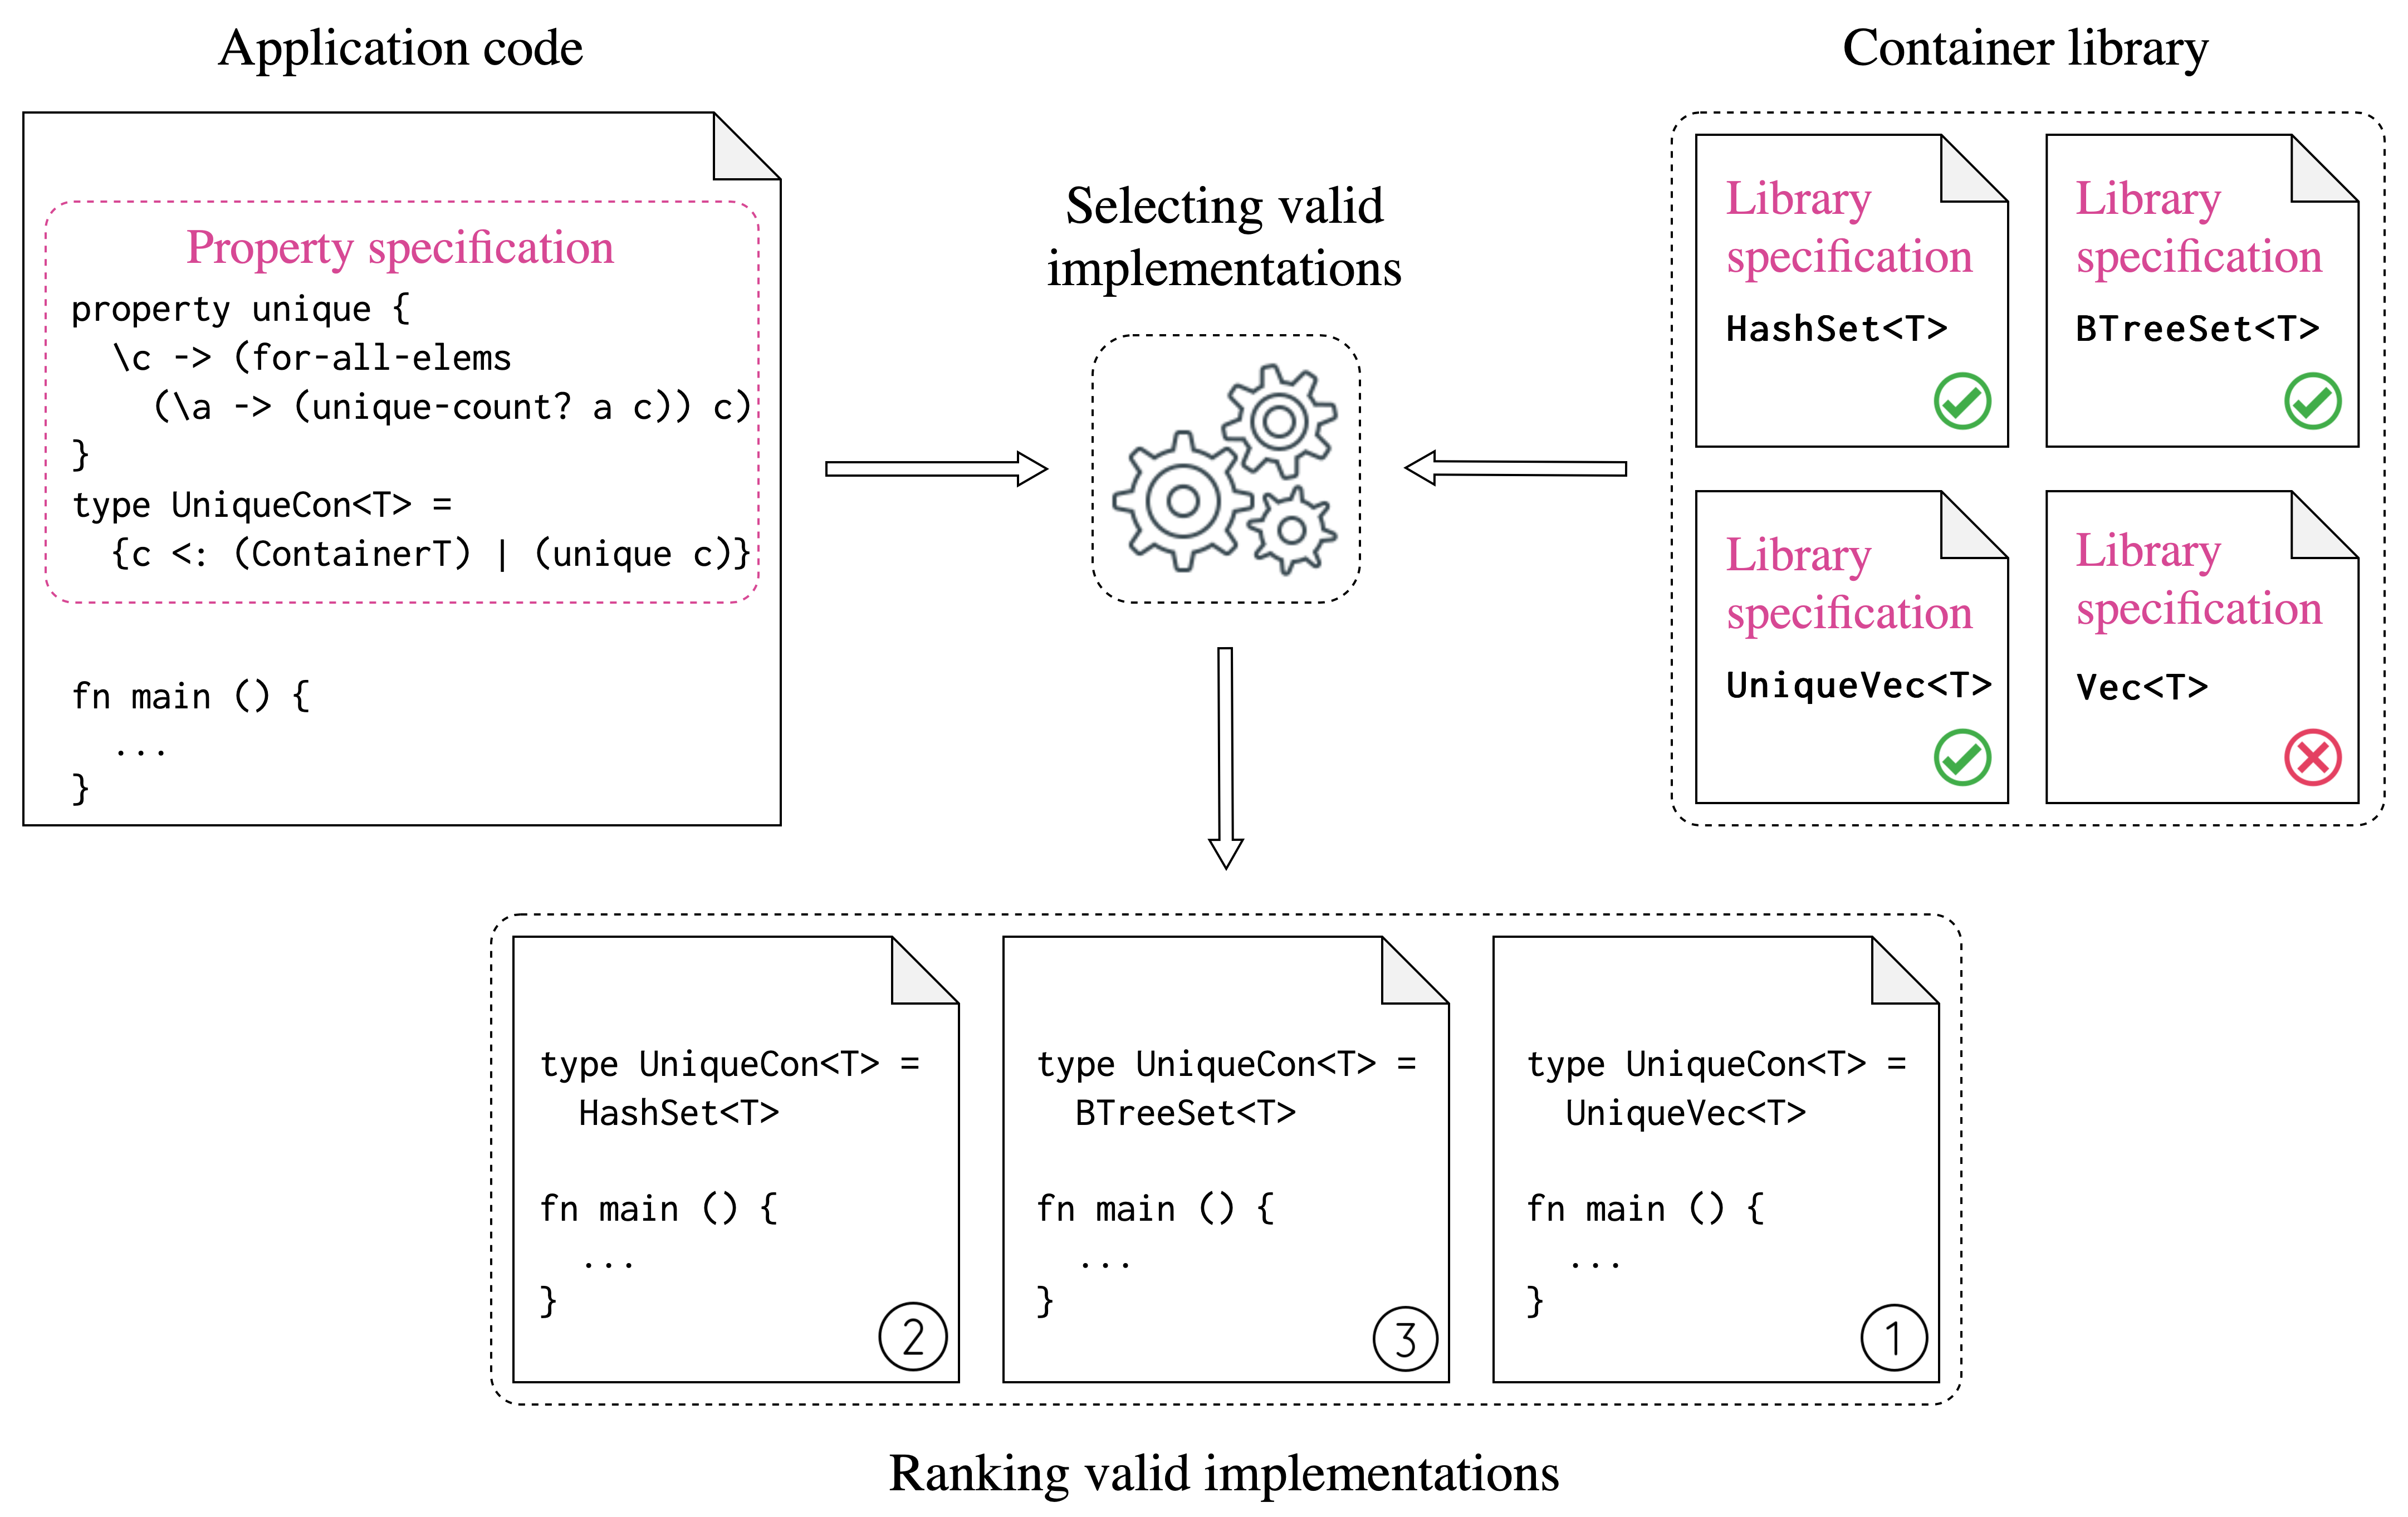
\includegraphics[width=0.95\textwidth]{./overview.png}
    \caption{The workflow of \Primrose{}:
    \emph{Property specifications} (top left), written and used by the application developer, are used to check which \emph{library specifications} (top right), written by library developers, satisfy them.
    Valid implementations (marked with a green check marks), are then ranked by their performance (bottom).
    }
    \label{overview:design}
\end{figure}

Given this code as input, \Primrose{} will, acting as 
a preprocessor, generate copies of the input code where the abstract type is instantiated into a valid concrete implementation that satisfies the expected properties. It determines 
which implementations are valid by consulting \emph{library specifications}, which are provided by library developers. These specifications abstract over concrete container implementations 
and provide a summary of their externally observable semantics. 
For each implementation, the library specification contains the pre- and post-conditions of each operation in terms of an abstract list model. We discuss these specifications in more detail in 
section~\ref{chap2:lib}. 

In our example in 
figure~\ref{overview:design}, the library specification of the \lstinline{Vec<T>} type indicates that it is not a suitable choice for \lstinline{UniqueCon<T>}, as it does not satisfy the required semantic property \lstinline{unique}.
We use a satisfiability modulo theories (SMT) solver for the selection process, which we discuss in section~\ref{chap2:select}.

Figure~\ref{overview:design} shows at the bottom a simplified version of the generated programs.
Note that in order to make \ref{overview:design} concise, we only show a simplified version of the generated programs with selected implementations that does not reflect how traits constrain available operations for interacting with the container type.
In our implementation, we ensure that only the container operations that the application developer specifies with syntactic properties are accessible in the generated program.
%
% After all valid container implementations are selected, \Primrose{} measures and ranks them according to their performance, and then selects the one providing the best performance for the program.
% We discuss the ranking in \ref{chap2:rank}.
%
Our current prototype of \Primrose{} focuses on ensuring the functional correctness of selecting container implementations based on desired properties.
Nevertheless, we have implemented a simple process that ranks valid implementations by their runtime performance.
Rankings by other non-functional metrics could easily be added to our design.
We provide discussion about code generation and ranking in section~\ref{chap2:rank}.

% Porting to other languages
% We discuss the portability of \Primrose{} in \ref{chap2:evaluation}.
% \paragraph{Using Rosette for Designing Specifications and the Selection Process}
\paragraph*{Using Rosette as the Common Language for Specifications and Selection}
\label{common-language}
The ``solver-aided programming language'' Rosette~\citep{rosette-lang, rosette-paper} is used as the common language in \Primrose{} for the formal parts.
Rosette is chosen for \Primrose{} due to its convenient interface to the Z3 SMT solver and the straightforward translation from \Primrose{} property specifications into Rosette.
Property specifications are used as verification conditions when selecting implementations by checking against library specifications which are directly encoded in Rosette. The selection process is done by interacting with the SMT solver via Rosette.


\paragraph*{Portability of \Primrose{}}
\label{implementation:portability}
Currently, we choose Rust as the target language to implement our idea. Application developers write the property specifications as a part of their Rust programs and \Primrose{} generates Rust code after processing specifications. 
However, \Primrose{} could easily be ported to many other languages, since property specifications, 
library specifications, and the process of selecting implementations are all language-agnostic and not attached to Rust's particular type system or language features.
Adapting property specifications into other languages only requires such languages to have a construct similar to Rust's traits, 
such as traits in Scala and interfaces in Java, allowing us to model syntactic properties. It would be straightforward to add new backends to \Primrose{} to 
generate code in these languages. Our library specifications are, by design, an abstraction over implementation details, describing the intended semantics of container operations without respect to 
their implementation. This means we can trivially adapt these specifications to container libraries from other languages, so long as our specifications remain an abstraction of the 
new implementations.  Thus, we anticipate that \Primrose{} could easily be adapted to produce code in any language with sufficient support for data abstraction, such as Java, Scala, Swift, or \Cpp.

\section{Property Specifications}
\label{chap2:prop}
The application developer specifies the desired behaviours of their required container with a \textit{property specification},
% that consists of \emph{semantic properties}, which refine the container type by a predicate, and \emph{syntactic properties}, which in Rust are traits specifying the operations that must be supported by the container and their types.
%
%The property specification of the type \lstinline{UniqueCon} from the example in \ref{overview:design} is:
for example, for the type \lstinline{UniqueCon} from figure~\ref{overview:design}:
\begin{lstlisting}[language=Rust, style=boxed, escapechar=!]
!\tikz[remember picture, overlay]\node [xshift=12.8cm, yshift=+.075cm, inner sep=0.075cm, rectangle] {\footnotesize\bfseries\texttt{Primrose}};!property unique 
  { \c -> (for-all-elems (\a -> (unique-count? a c)) c) }
type UniqueCon<T> = {c <: (ContainerT) | (unique c)}
\end{lstlisting}

We first define the \emph{semantic property} \lstinline{unique} using a \emph{predicate}.
In our specification language, such predicates have type $\mathit{Con}\langle\tau\rangle \to \mathit{Bool}$, where $\mathit{Con}\langle\tau\rangle$ is a placeholder that is resolved into a concrete container type by 
the selection process. The combinator \lstinline{for-all-elems} is part of a library enabling to write predicates for individual container elements. The predicate \lstinline{unique-count?} holds if and only if the given element occurs exactly once in the container. These combinators and predicates are explained in section~\ref{chap2:prop:semantic}.

With the defined \emph{semantic property} \lstinline{unique}, we can then declare the container type \lstinline{UniqueCon<T>}. 
The first part of the declaration specifies the syntactic property that must be satisfied by the container type, in the form of the trait 
\lstinline{ContainerT}. Specifically, \lstinline{c <: (ContainerT)} says that the type of the container \lstinline{c} must implement the trait \lstinline{ContainerT}, which specifies a set of basic container operations. 
The second part of the declaration \emph{refines} our container type by the predicate \lstinline{unique}, stating that the property must be invariant across all container operations.
Properties may also be composed. For multiple syntactic properties, we specify a list of traits (\lstinline{c <: (T1, T2)}) that the container type implements. For multiple semantic properties, we use conjunction, i.e.\ \lstinline{((p1 c) and (p2 c))}.

\begin{figure}[t]
  \begin{alignat*}{3}
  \mathrm{Literals} \quad 
  &l \ &\metaDef \quad &\mathit{true} \cmid \mathit{false}
  \\[-.25em]
  \mathrm{Terms} \quad
  &t \ &\metaDef \quad &l \cmid x \cmid \lambda x.\ t \cmid t\ t
  \\[-.25em]
  %\mathrm{Predicate} \quad 
  %&p \ &\metaDef \quad &\lambda x.\ t
  %\\[-.25em]
  \mathrm{Refinement} \quad 
  &r \ &\metaDef \quad &t \cmid r \wedge r
  \\[-.25em]
  \mathrm{Container\ Type\ Declarations} \quad 
  &c \ &\metaDef \quad &\{v \ \metaBound\ B \mid r\}
  \\[-.25em]
  \mathrm{Simple\ Types} \quad 
  &\sigma \ &\metaDef \quad &\mathit{Bool} \cmid T \cmid \mathit{Con}\langle\sigma\rangle 
  \\[-.25em]
  \mathrm{Types} \quad 
  &\tau \ &\metaDef \quad &\sigma \cmid \tau \to \tau \cmid \forall T \metaBound B .\ \tau
  \\[-.25em]
  \mathrm{Bounds} \quad
  &B \ &\metaDef \quad &\mathit{trait\_name} \cmid B \sep B
  %\\[-.25em]
  %\mathrm{Kinds} \quad 
  %&\kappa \ &\metaDef \quad &\mathsf{type} \cmid \kappa_1 \Rightarrow \kappa_2
  \end{alignat*}
  \caption{The syntax of property specifications. $T$ is the type variable, ranging over element types of the target language, which is Rust in this case.}
  \label{prop:syntax}
\end{figure}

Figure~\ref{prop:syntax} shows the syntax of the \Primrose{} property specification language. Formally, the specification language is a variant of the polymorphic $\lambda$-calculus~\citep{DBLP:conf/programm/Reynolds74, DBLP:journals/tcs/Girard86}, with 
restrictions on the use of polymorphism to enable implicit type inference~\citep{hindley1969principal, MILNER1978348}.
This type system guarantees termination, making specifications easier to analyse and straightforward to translate into SMT verification conditions in Rosette.
The translation into Rosette is straightforward, as terms in the \Primrose{} property specification language (literals, variables, lambdas, and function application) are translated into their counterparts in the functional Rosette language. 

\subsection{Syntactic Properties as Traits}
\label{chap2:prop:syntactic}
In our \Primrose{} prototype, we encode syntactic properties as Rust traits, specifying the operations needed by the application developer to interact with a container. 
Traits are defined in Rust and lifted into our property specification language. For instance, the trait \lstinline|ContainerT| introduced above is implemented as:
\begin{lstlisting}[language=Rust, style=boxed, escapechar=!]
!\tikz[remember picture, overlay]\node [xshift=12.95cm, yshift=+.075cm, inner sep=0.075cm, rectangle] {\footnotesize\bfseries\texttt{Rust}};!pub trait ContainerT<T> {
  fn len(&self) -> usize;
  fn contains(&self, x: &T) -> bool;
  fn is_empty(&self) -> bool;
  fn insert(&mut self, elt: T);
  fn clear(&mut self);
  fn remove(&mut self, elt: T) -> Option<T>;}
\end{lstlisting}

By writing \lstinline{c <: ContainerT}, the application developer indicates that they expect the container type selected by \Primrose{} to include implementations for all operations in the trait \lstinline{ContainerT}. 
Thus, after executing \Primrose{}, \mylstinline{UniqueCon<T>} will be resolved into a concrete container type that implements the trait \lstinline{ContainerT}.

As mentioned, we can also declare a container type that satisfies multiple syntactic properties. For instance, suppose that in addition to \lstinline{ContainerT}, we would like our container to also satisfy the syntactic property \lstinline{IndexableT}:
\begin{lstlisting}[language=Rust, style=boxed, escapechar=!]
!\tikz[remember picture, overlay]\node [xshift=12.95cm, yshift=+.075cm, inner sep=0.075cm, rectangle] {\footnotesize\bfseries\texttt{Rust}};!pub trait IndexableT<T> {
  fn first(&self) -> Option<&T>;
  fn last(&self) -> Option<&T>;
  fn nth(&self, n: usize) -> Option<&T>;
}
\end{lstlisting}

With just \lstinline{ContainerT}, there is no way to observe the \emph{ordering} of elements in the container, but with \lstinline{IndexableT} there is, as we can now select elements based on their position.
By composing our new syntactic property \lstinline{IndexableT} with \lstinline{ContainerT} we can now 
specify a container of unique elements where the order can be observed:
\begin{lstlisting}[language=Rust, style=boxed, escapechar=!]
!\tikz[remember picture, overlay]\node [xshift=12.8cm, yshift=+.075cm, inner sep=0.075cm, rectangle] {\footnotesize\bfseries\texttt{Primrose}};!type UniqueIndexableCon<T> = 
  { c <: (ContainerT, IndexableT) | (unique c) }
\end{lstlisting}

Semantic properties, such as \lstinline{unique}, must be invariant across all operations from all syntactic properties required of the container.
%\todo[author=Michel]{Removed the following snipped, as I think this is redundant}

\subsection{Semantic Properties as Predicates}
\label{chap2:prop:semantic}
As mentioned, semantic properties are predicates that are used to construct refinements for container types; each declared container type in the form $\{v \ \metaBound\ B \mid r\}$ is a \textit{refinement type}, i.e.\ a type circumscribed by a logical predicate~\citep{10.1145/113445.113468}. When the predicates are in SMT-decidable logic, they can be statically checked~\citep{10.1145/1863543.1863560}.
Such techniques are used in programming languages like Liquid Haskell and F*, where they are used to facilitate verification of program correctness. 
For instance, in Liquid Haskell, we may define a refinement type \lstinline{UniqueList} representing a list of unique elements as:
% , caption={Unique List in Liquid Haskell}, captionpos=b, label=prop:lh-uniquelist]
\begin{lstlisting}[language=haskell, style=boxedlst, escapechar=!]
!\tikz[remember picture, overlay]\node [xshift=12.5cm, yshift=+.075cm, inner sep=0.075cm, rectangle] {\footnotesize\bfseries\texttt{Liquid Haskell}};!{-@ measure unique @-}
unique :: (Ord a) => [a] -> Bool
unique [] = True
unique (x:xs) = unique xs && not (S.member x (elts xs))
{-@ type UniqueList a = {v:[a] | unique v} @-}
\end{lstlisting}

\noindent While our syntax for type refinements strongly resembles Liquid Haskell, our refinement types are slightly different, and serve a different purpose.
Firstly, Liquid Haskell's refinements 
are attached to a \emph{concrete type}, in this case a list (written \lstinline{[a]}), whereas our refinements are attached to an abstract container type, which is then resolved by \Primrose{} into a concrete 
implementation. Secondly, Liquid Haskell 
uses type refinements for the purpose of \emph{correctness}: If a list is declared to have type \lstinline{UniqueList}, the Liquid Haskell verifier will check that it satisfies the predicate \lstinline{unique}. 
The \lstinline{notUniqueList} shows that it will report an error at compile time if a given list contains duplicates.
\begin{lstlisting}[language=haskell, style=boxedlst, escapechar=!]
!\tikz[remember picture, overlay]\node [xshift=12.5cm, yshift=+.075cm, inner sep=0.075cm, rectangle] {\footnotesize\bfseries\texttt{Liquid Haskell}};!{-@ notUniqueList :: UniqueList Int @-}
notUniqueList::[Int]
notUniqueList = [3, 1, 2, 3]
\end{lstlisting}
Our work instead uses type refinements to specify the semantic requirements of the application developer to guide selection of valid concrete implementations.
Once all valid implementations have been found, \Primrose{} simply selects the implementation providing the best performance for the application developer.
In short, rather than to aid verification, we use refinement types to help application developers optimise their programs. We give more details on the selection process in section~\ref{chap2:select}.

\paragraph*{Combinators and Predicate Functions} Demonstrated by our examples, \Primrose{} provides a set of combinators and predicate functions to facilitate writing of property specifications. 
These combinators and predicate functions are defined in Rosette and then imported into our property 
specification language.  In the semantic property \lstinline{unique}, the combinator \lstinline{for-all-elems} is used to specify that the predicate \lstinline{unique-count?} must hold for all elements inside the container. 
The type of the combinator \lstinline{for-all-elems} is $\mathit{Con}\langle\tau\rangle \to (\tau \to \mathit{Bool}) \to \mathit{Bool}$, meaning this combinator takes in two arguments, the first of which is a container and the second of which is a predicate on the elements of that container, and eventually returns a boolean value.

For the purposes of checking, we represent containers $\mathit{Con}\langle\tau\rangle$ abstractly in Rosette as lists. We discuss this list abstraction and justify it in section~\ref{chap2:lib}.
With such a list abstraction, we are able to straightforwardly implement our \lstinline{for-all-elems} combinator with a list fold operation:
\begin{lstlisting}[language=racket, style=boxed, label=prop:combinator-unary, escapechar=!] 
!\tikz[remember picture, overlay]\node [xshift=12.8cm, yshift=+.075cm, inner sep=0.075cm, rectangle] {\footnotesize\bfseries\texttt{Rosette}};!(define (for-all-elems c fn)
    (foldl elem-and #t (map (lambda (a) (fn a)) c)))
\end{lstlisting}

We also provide some combinators for applying \emph{relations} between elements in a container. For instance, the combinator \mylstinline{for-all-consecutive-pairs}:
\begin{align}
    \label{prop:combinator-pair}
    \texttt{for-all-consecutive-pairs}\; :\; \mathit{Con}\langle\tau\rangle \to (\tau \to \tau \to \mathit{Bool}) \to \mathit{Bool}
\end{align}
Unlike \lstinline{for-all-elems}, this combinator gives a binary relation between elements, and checks that this relation holds between any two consecutive elements in a container.

With the combinator \lstinline{for-all-consecutive-pairs} and the predicates \lstinline{geq?} and \lstinline{leq?}, we can define properties like \lstinline{ascending} and \lstinline{descending}, which specify particular orderings of elements in a container:
\begin{lstlisting}[language=Rust, style=boxed, escapechar=!]
!\tikz[remember picture, overlay]\node [xshift=12.8cm, yshift=+.075cm, inner sep=0.075cm, rectangle] {\footnotesize\bfseries\texttt{Primrose}};!property ascending { \c -> (for-all-consecutive-pairs c leq?) }
property descending { \c -> (for-all-consecutive-pairs c geq?) }
\end{lstlisting}

Besides the set of combinators and predicate functions predefined in \Primrose{}, application developers may also provide customised functions by providing Rosette definitions and importing them into our property specification language. 

\paragraph*{Composition of semantic properties} As shown in figure~\ref{prop:syntax}, we can compose semantic properties in a container type declaration with conjunction.
For instance, to declare a container type with elements arranged in \emph{strictly} ascending order, i.e., both \lstinline{unique} and \lstinline{ascending} properties must hold, we can write the following:
\begin{lstlisting}[language=Rust, style=boxed]
!\tikz[remember picture, overlay]\node [xshift=12.8cm, yshift=+.075cm, inner sep=0.075cm, rectangle] {\footnotesize\bfseries\texttt{Primrose}};!type StrictlyAscendingCon<T> = 
  { c <: (ContainerT) | ((unique c) and (ascending c)) }
\end{lstlisting}
The conjunction \lstinline|and| is directly translated into a conjunction operation in Rosette.

\subsection{The Interaction between Semantic Properties and Syntactic Properties}
\label{chap2:prop:semantic-syntactic}
All semantic properties we have seen so far have been invariants across all operations, but 
some semantic properties relate to specific operations given by syntactic properties. 
For instance, when specifying a stack container type providing operations \lstinline{push} and \lstinline{pop} with the expected last-in-first-out (LIFO) property.
% on top of the trait \lstinline{ContainerT} specifying basic container operations, 
Firstly, we define a trait specifying operations \lstinline{push} and \lstinline{pop}, namely \lstinline{StackT}:
\begin{lstlisting}[language=Rust, style=boxed, caption=The trait \mylstinline{StackT} specifying operations \mylstinline{push} and \mylstinline{pop}, captionpos=t, label=prop:spec-stackt, escapechar=!]
!\tikz[remember picture, overlay]\node [xshift=12.95cm, yshift=+.075cm, inner sep=0.075cm, rectangle] {\footnotesize\bfseries\texttt{Rust}};!pub trait StackT<T> {
  fn push(&mut self, elt: T);
  fn pop(&mut self) -> Option<T>;
}
\end{lstlisting}
Secondly, we define the semantic property \lstinline{lifo} for containers that implement \lstinline{StackT}:
\begin{lstlisting}[language=Rust, style=boxed, caption=The semantic property LIFO, captionpos=t, label=prop:spec-lifo, escapechar=!]
!\tikz[remember picture, overlay]\node [xshift=12.8cm, yshift=+.075cm, inner sep=0.075cm, rectangle] {\footnotesize\bfseries\texttt{Primrose}};!property lifo { \c <: StackT -> (forall \x. pop (push c x) == x) }
\end{lstlisting}
\noindent
Unlike previously, this semantic property includes a requirement that the given container implements the trait \lstinline{StackT}, enabling us to refer to the operations \lstinline{pop} and \lstinline{push} inside the semantic property. In this definition, \lstinline{forall} is a combinator with type:
\begin{align}
    \label{prop:combinator-forall}
    \texttt{forall}\; :\; \forall x. \,(x \to \mathit{Bool}) \to \mathit{Bool}
\end{align}
This combinator is implemented with the \lstinline{forall} procedure defined in Rosette's library, which serves as a construct for creating universally quantified formulae.

Armed with the trait \lstinline{StackT} and the semantic property \lstinline|lifo|, we can combine all these elements and declare our stack type as follows:
%  caption=The container type with stack operations satisfying the semantic property LIFO, captionpos=b,
\begin{lstlisting}[language=Rust, style=boxed, escapechar=!]
!\tikz[remember picture, overlay]\node [xshift=12.8cm, yshift=+.075cm, inner sep=0.075cm, rectangle] {\footnotesize\bfseries\texttt{Primrose}};!type StackCon<T> = {c <: (ContainerT, StackT) | (lifo c)}
\end{lstlisting}

In the next section, we will discuss how library developers write specifications for their container implementations.

%\Primrose{} selects among these library specifications the ones that satisfy the properties required by application developers.

\section{Library Specifications}
\label{chap2:lib}
% show full spec
% unique + lifo
% verification
% no good rust semantic framework for verification yet; rust belt in dev.
%
% TODO: Should we remove this to streamline the presentation (this feels a bit like a re-motivation of the points we made already in the introduction)
% It is not feasible to select container implementations directly by analysing their Rust source code and checking if they satisfy the properties specified by the application developer.
% Rust is a Turing-complete, general purpose programming language with a complex semantics, and its container libraries 
% are typically highly optimised, making extensive use of unsafe code. Doing such a broad analysis precisely and automatically is very hard even for the most advanced of static analyses.
% Instead, we write 
\emph{Library specifications} abstract over Rust container implementations, providing a clear definition of intended semantics of each operation, without respect to performance or implementation details. 
This approach allows us to select container implementations by simply checking their library specifications, rather than their full implementations, against the properties specified by the application developer.
Moreover, using specifications which are abstracted from implementations makes \Primrose{} easy to repurpose for programming languages other than Rust, as the same specifications would apply, with minimal or no modification, to container libraries written in any other language. 

By encoding these specifications into \emph{property based tests}, which validate container implementations against their library specifications (section~\ref{chap2:evaluation:testing}), we ensure the selected implementations indeed satisfy a required property specification. Since these library specifications form a \emph{functional correctness} specification for each operation, they could also be used in future as the basis of full functional correctness verification with a verification framework for Rust~\citep{rustbelt-paper}, but this is out of scope for \Primrose{}.

\subsection{The Basic Design of Library Specifications}
\label{chap2:lib:design}
Library specifications of concrete container implementations are developed based on Hoare logic~\citep{10.1145/363235.363259}.
For each concrete container implementation, we provide a set of \emph{Hoare triples}, one for each operation. A Hoare triple of the form
$\{\phi\}\; \mathsf{op} \;\{\psi\}$ states that if the \textit{precondition} $\phi$ holds and the operation $\mathsf{op}$ is executed, then the \textit{postcondition} $\psi$ will hold.
These conditions are predicates on the state of the program. In our case, the state contains the container, plus any other inputs and outputs of the operation $\mathsf{op}$.

As mentioned in section~\ref{chap2:overview}, we model the container as a list in Rosette for \Primrose{}'s library specifications. The list is a model to convey the intended semantics, and does not proscribe anything about the implementation --- the implementation is free to represent 
data in any chosen structure. For example, a set data type may be implemented with a binary search tree, but will still be specified with a list. 
These model lists are a simple abstraction, easy to analyse, with which all container operations can be specified.

\paragraph*{Library Specifications Convey the Intended Semantics for Implementations} It is important that all possible executions of a concrete implementation should be captured by its library specification. Otherwise in the process of selecting implementations by checking if their library specifications match the required semantic property, \Primrose{} could select an unsatisfying implementation. More formally, a proof of functional correctness of an implementation w.r.t. its specification would take the form of a data refinement~\citep{de_roever_engelhardt_1998},
where each value of the concrete container type is related to our list model by an \emph{abstraction function} $\alpha$, and our specification on lists is shown to contain all possible behaviours 
of the concrete implementation using a \emph{forward simulation}:
% \begin{figure}[!ht]
\vspace{-.5em}
\begin{center}
  $\begin{array}{c}\alpha^{-1};\mathsf{op(\textit{C})}  \subseteq
  \mathsf{op(\textit{A})}; \alpha^{-1}\quad\\\text{\footnotesize (where ; is forward composition of relations} \\\text{\footnotesize and $\alpha^{-1}$ is the inverse relation of $\alpha$)}\end{array}$
\begin{tikzcd}[row sep=1.2cm,column sep=1.2cm,inner sep=0.7ex, cramped]
\circ
\arrow[Mapsto]{r}[name=U]{\textsf{op(\textit{A})}}
\arrow[dr, rounded corners,
       to path={ ([xshift=1.3ex,yshift=-0.5ex]\tikztostart.south) |- ([yshift=1.3ex,xshift=-0.5ex]\tikztotarget.west)}]
\arrow[dr, rounded corners,
       to path={ ([yshift=-1.3ex,xshift=0.5ex]\tikztostart.east) -| ([xshift=-1.3ex, yshift=0.5ex]\tikztotarget.north)}]
&
\circ
\\
\bullet
\arrow[dashed]{u}{\alpha}
\arrow[swap, Mapsto]{r}[name=D]{\textsf{op(\textit{C})}}
&
\bullet
\arrow[swap,dashed]{u}{\alpha}
\arrow[to path={(U) node[midway,scale=1.5] {\rotatebox[origin=c]{90}{$\subseteq$}}  (D)}]{}
\end{tikzcd}
\end{center}
% \caption{Forward simulation} \label{lib:forward-simulation}
% \end{figure}

\noindent Here, $\mathsf{op(\textit{C})}$ denotes the concrete implementation of our operation $\mathsf{op}$, represented as a relation from inputs to outputs.
The abstract operation $\mathsf{op(\textit{A})}$ is the maximal relation satisfying the Hoare triple given in our library specification, and $\alpha$ is a suitable abstraction function that 
flattens a concrete container into a list. 

If a forward simulation is shown for all operations, we can then conclude that each possible execution with the concrete container implementation has a corresponding execution with an abstract list, thus the specification accurately captures the implementation's semantics.

For instance, a binary search tree $T$ can be abstracted to a sorted list $L$ by an abstraction function $\mathit{inorder}$ that does an in-order traversal. For each operation interacting with $T$, there exists a corresponding operation at the abstract level defined using $L$. 
Take the operation $\mathsf{insert(\textit{T},x)}$, which inserts an element $x$ into a binary search tree $T$. We can abstract such an operation to $\mathsf{insert(\textit{L},x)}$ which inserts $x$ at the right location in a sorted list. The relation between these two operations is shown by this diagram:
\vspace{-.4em}
\begin{center}
 % $\begin{array}{c}\mathit{inorder}(\mathsf{insert}(\textit{T},x)) \mathit{inorder}^{-1};\mathsf{len(\textit{T})}  \subseteq
 % \mathsf{len(\textit{L})}; inorder^{-1}\quad\end{array}$
\begin{tikzcd}[row sep=1.2cm,column sep=1.2cm,inner sep=0.7ex, cramped]
\circ
\arrow[Mapsto]{r}[name=U]{\textsf{insert(\textit{L},x)}}
\arrow[dr, rounded corners,
       to path={ ([xshift=1.3ex,yshift=-0.5ex]\tikztostart.south) |- ([yshift=1.3ex,xshift=-0.5ex]\tikztotarget.west)}]
\arrow[dr, rounded corners,
       to path={ ([yshift=-1.3ex,xshift=0.5ex]\tikztostart.east) -| ([xshift=-1.3ex, yshift=0.5ex]\tikztotarget.north)}]
&
\circ
\\
\bullet
\arrow[dashed]{u}{\mathit{inorder}}
\arrow[swap, Mapsto]{r}[name=D]{\textsf{insert(\textit{T},x)}}
&
\bullet
\arrow[swap,dashed]{u}{\mathit{inorder}}
\arrow[to path={(U) node[midway,scale=1.5] {\rotatebox[origin=c]{90}{$\subseteq$}}  (D)}]{}
\end{tikzcd}
\end{center}
\vspace{-.4em}
\noindent In this work, we specified four container implementations from Rust's standard library (\lstinline!Vec!,\,\lstinline!LinkedList!,\,\lstinline!HashSet!,\,\lstinline!BTreeSet!) and four custom container implementations (\lstinline!SortedVec!,\,\lstinline!LazySortedVec!,\,\lstinline!UniqueVec!,\,\lstinline!LazyUniqueVec!) by abstracting them into a list model.
As we discuss in section~\ref{chap2:lib:abstracting}, library specifications abstract over some implementation details, and, thus, \lstinline!Vec! and \lstinline!LinkedList! share the same specifications, as do the eager and lazy \lstinline!SortedVec! and \lstinline!UniqueVec! implementations.
For each specification, we define a suitable abstraction function for forward simulation which, while not needed for selection, is used for property-based testing to justify that a concrete implementation satisfies the intended semantics described by its library specification.

\paragraph*{Completeness of Library Specifications} 
While it is important to ensure that library specifications indeed convey the intended semantics of the implementation, \emph{completeness} of library specifications is also important. Without completeness, \Primrose{} could possibly rule out perfectly valid implementations because it cannot prove that the required semantic properties are preserved for an operation of which the specification is incomplete. 

Our approach easily ensures completeness when each operation is specified by a \emph{deterministic} model operation. Forward simulation states that every execution of the concrete implementation has a corresponding execution in the abstract operation, while determinism states that such correspondence is one-to-one, i.e., each abstract execution also has a corresponding concrete one.
Thus, just as forward simulation states that each property established for an abstract operation applies also (via the inverse of the abstraction function $\alpha^{-1}$) to a concrete implementation, completeness states that each property established for a concrete implementation applies (via the abstraction function $\alpha$) to the abstract operation. With both completeness and forward simulation, we ensure that \emph{all} valid implementations and \emph{only} the valid implementations are selected by \Primrose{}.

There are many other availiable approaches for modelling library specifications, for instance, the axiomatic approach used in algebraic specifications for abstract data types \cite{WIRSING1990675}, specifying the behaviour of operations as a set of equational axioms that relate various operations.
However, it is hard to ensure the completeness of algebraic specifications, as it is hard capture all behaviours of all operations by a set of equations.  

\subsection{The Library Specification of A \texttt{LinkedList}}
\label{chap2:lib:list}
Rust's \lstinline{LinkedList} is a doubly-linked list. The abstraction function to convert it into a logic list is straightforward: Collect all nodes' values with previous and next pointers.

Firstly, we specify the insertion operation, \lstinline|LinkedList::insert|, of which the type signature is:
% caption=The signature of \mylstinline{LinkedList::insert}, captionpos=b, label=lib:sig-list-insert
\begin{lstlisting}[language=Rust, style=boxed, escapechar=!]
!\tikz[remember picture, overlay]\node [xshift=12.95cm, yshift=+.075cm, inner sep=0.075cm, rectangle] {\footnotesize\bfseries\texttt{Rust}};!fn insert(&mut self, elt: T) {...}
\end{lstlisting}
\noindent
Since variables in Rosette are immutable, in the corresponding abstract insertion operation, we alter the type to return a new list instead of altering the list in-place\footnote{Rosette is untyped, but this is morally the type signature.}:
%, caption=The signature of the abstract operation corresponding to \mylstinline{LinkedList::insert}, captionpos=b, label=lib:sig-abs-insert
\begin{lstlisting}[language=racket, style=boxed]
!\tikz[remember picture, overlay]\node [xshift=12.8cm, yshift=+.075cm, inner sep=0.075cm, rectangle] {\footnotesize\bfseries\texttt{Rosette}};!abs-insert: List<T> -> T -> List<T>
\end{lstlisting}
We can then provide the specification of \lstinline|LinkedList::insert| with respect to its corresponding abstract operation, the maximal relation satisfying the Hoare triple:
\begin{align}
\label{lib:spec-list-insert}
\{xs_0.\ \texttt{\small true}\}~\texttt{abs-insert}~\{xs_0\ x\ xs.\ xs = \texttt{\small model-insert}\ xs_0\ x\}
\end{align}
Here, $xs_0$ refers to the initial value of the container, $xs$ refers to the resultant container, and $x$ is the element we insert. The function \lstinline|model-insert| is defined in Rosette on lists:
%, caption=The model insertion operation, captionpos=b, label=lib:logic-list-insert
\begin{lstlisting}[language=racket, style=boxed]
!\tikz[remember picture, overlay]\node [xshift=12.8cm, yshift=+.075cm, inner sep=0.075cm, rectangle] {\footnotesize\bfseries\texttt{Rosette}};!(define (model-insert xs x) (append xs (list x)))
\end{lstlisting}
The postcondition states that we expect applying the insertion operation to a container to produce the same result as the result produced by \lstinline|model-insert| function. In library specifications, defining such \emph{model operations} is a common technique to simplify writing postconditions. 

Similarly, we also provide the specification for the operation \lstinline{LinkedList::contains}:
%, caption=The signature of \mylstinline{LinkedList::contains}, captionpos=b, label=lib:sig-list-contains
\begin{lstlisting}[language=Rust, style=boxed, escapechar=!]
!\tikz[remember picture, overlay]\node [xshift=12.95cm, yshift=+.075cm, inner sep=0.075cm, rectangle] {\footnotesize\bfseries\texttt{Rust}};!fn contains(&self, x: &T) -> bool {...}
\end{lstlisting}
\noindent
In our corresponding abstract operation, in addition to the boolean value indicating whether the given element \lstinline|x| is present or not, the input container is also returned, as we would like to express the input container is not mutable, its value remains unchanged after this operation. Also, since the underlying value with type \lstinline|T| is given by an immutable reference \lstinline|&T|, in the abstract operation we treat the immutable reference \lstinline|&T| as simply \lstinline|T|. The signature of the abstract operation is shown below:
\begin{lstlisting}[language=racket, style=boxed, caption=The signature of the abstract operation corresponding to \mylstinline{LinkedList::contains}, captionpos=t, label=lib:sig-abs-contains]
!\tikz[remember picture, overlay]\node [xshift=12.8cm, yshift=+.075cm, inner sep=0.075cm, rectangle] {\footnotesize\bfseries\texttt{Rosette}};!abs-contains: List<T> -> T -> (List<T>, bool)
\end{lstlisting}
The Hoare triple that serves as the specification of \lstinline|LinkedList::contains| is:
\begin{align}
\label{lib:spec-list-contains}
\{xs_0.\ \texttt{\small true}\}\ \texttt{abs-contains}\ \{xs_0\ x\ xs\ r.\ (xs, r) = \texttt{\small model-contains}\ xs_0\ x\}
\end{align}
Note that in this specification, the model operation \lstinline|model-contains| defined in listing~\ref{lib:logic-list-contains} has the same type signature as the abstract operation shown in listing~\ref{lib:sig-abs-contains}. It also returns a pair of values: the output list, which is always equal to the input list, and a boolean value indicating if the element is present in the list.
\begin{lstlisting}[language=racket, style=boxed, caption=The model operation for checking an element's containment, captionpos=t, label=lib:logic-list-contains]
!\tikz[remember picture, overlay]\node [xshift=12.8cm, yshift=+.075cm, inner sep=0.075cm, rectangle] {\footnotesize\bfseries\texttt{Rosette}};!(define (model-contains xs x)
  (cond [(list? (member x xs)) (cons xs #t)]
        [else (cons xs #f)]))
\end{lstlisting}
Because \lstinline|model-contains| returns the unchanged list, it specifies that the operation \lstinline|LinkedList::contains| should not change the list. 

The library specification of the list removal operation is slightly more complicated, we use \lstinline|T?| to denote that a type may be \lstinline|null| to express Rust's \lstinline{Option<T>} type, which is the return type of \lstinline|LinkedList::remove|. 
The type signature of \lstinline|LinkedList::remove| is shown below:
%, caption=The type signature of \mylstinline{LinkedList::remove}, captionpos=b, label=lib:sig-list-remove
\begin{lstlisting}[language=Rust, style=boxed, escapechar=!]
!\tikz[remember picture, overlay]\node [xshift=12.95cm, yshift=+.075cm, inner sep=0.075cm, rectangle] {\footnotesize\bfseries\texttt{Rust}};!fn remove(&mut self, x: T) -> Option<T> {...}
\end{lstlisting}
\noindent
This operation removes the first occurrence of an element from the given linked list and returns it. If the linked list does not contain the element, \lstinline|None| is returned and the list remains unchanged.
The signature of the corresponding abstract operation is:
%, caption=The signature of the abstract operation corresponding to \mylstinline{LinkedList::remove}, captionpos=b, label=lib:sig-abs-remove
\begin{lstlisting}[language=racket, style=boxed]
!\tikz[remember picture, overlay]\node [xshift=12.8cm, yshift=+.075cm, inner sep=0.075cm, rectangle] {\footnotesize\bfseries\texttt{Rosette}};!abs-remove: List<T> -> T -> (List<T>, T?)
\end{lstlisting}
The model removal operation has the same signature as the abstract operation. We return \lstinline|null| in Rosette for the \lstinline|None| case:
%, caption=The model removal operation, captionpos=b, label=lib:logic-list-remove
\begin{lstlisting}[language=racket, style=boxed]
!\tikz[remember picture, overlay]\node [xshift=12.8cm, yshift=+.075cm, inner sep=0.075cm, rectangle] {\footnotesize\bfseries\texttt{Rosette}};!(define (model-remove xs x) 
  (cond [(list? (member x xs)) (cons (remove x xs) x)]
        [else (cons xs null)]))
\end{lstlisting}
Again, we return a pair of the resulting list and the element being removed. Then we provide the library specification of \lstinline|LinkedList::remove|:
\begin{align}
\label{lib:spec-list-remove}
\{xs_0.\ \texttt{\small true}\}\ \texttt{abs-remove}\ \{xs_0\ x\ xs\ r.\ (xs, r) = \texttt{\small model-remove}\ xs_0\ x\}
\end{align}
To provide a complete specification of \lstinline|LinkedList|, the library developer must ensure that each operation of the \lstinline|LinkedList| is specified by a trait, and for each operation in each trait the \lstinline|LinkedList| implements, specifications similar to the above are provided.

\subsection{The Library Specification of A \texttt{BTreeSet}}
\label{chap2:lib:btree}
For the \lstinline|LinkedList| it is intuitive to use a logic list as a model, as they are both lists. However, even for non-linear structures such as trees, we can still use logic lists as a model. 
Rust's \lstinline|BTreeSet| is a set implemented using a b-tree.
All elements are unique and arranged in ascending order. Thus, our list model of the b-tree is simply a sorted list in ascending order, where uniqueness of elements is preserved.
The abstraction function $\alpha$ that converts the \lstinline|BTreeSet| to our list model is simply an in-order traversal.

The first example to be illustrated is again the specification of the insertion operation with signature:
%, caption=The signature of \mylstinline{BTreeSet::insert}, captionpos=b, label=lib:sig-tree-insert
\begin{lstlisting}[language=Rust, style=boxed, escapechar=!]
!\tikz[remember picture, overlay]\node [xshift=12.95cm, yshift=+.075cm, inner sep=0.075cm, rectangle] {\footnotesize\bfseries\texttt{Rust}};!pub fn insert(&mut self, value: T) {...}
\end{lstlisting}
\noindent
The signature of the abstract insert operation on our model lists is the same as for \lstinline{LinkedList::insert}.
% resembles the abstraction of \lstinline{LinkedList::insert}:
%, caption=The signature of the abstract operation corresponding to \mylstinline{BTreeSet::insert}, captionpos=b, label=lib:sig-abs-insert-tree
% \begin{lstlisting}[language=racket, style=boxed]
% abs-insert: List<T> -> T -> List<T>
% \end{lstlisting}
The specification of \lstinline{abs-insert} for \lstinline|BTreeSet|, however, differs from that of \lstinline|LinkedList|, as we must maintain ordering and uniqueness of elements:
\begin{align}
\label{lib:spec-tree-insert}
\{xs_0.\ xs_0 = \texttt{\small dedup}\ (\texttt{\small sort}\ xs_0\ \texttt{\small<})\}~\texttt{abs-insert}~\{xs_0\ x\ xs.\ xs = \texttt{\small model-insert}\ xs_0\ x\}
\end{align}
As before, $x$ is the element to be inserted, and $xs_0$ and $xs$ are lists modelling the container (via the in-order traversal function $\alpha$) before and after the \lstinline|abs-insert| operation respectively. 
We place an assertion $xs_0 = \texttt{\small dedup}\ (\texttt{\small sort}\ xs_0\ \texttt{\small<})$ in the precondition requiring that the model $xs_0$ to be a sorted list of unique elements. 
While this precondition should always be satisfied by an in-order traversal of a valid b-tree, we do not want our abstraction to constrain the implementation's behaviour if the data invariants of the b-tree are violated --- given a malformed b-tree, the 
implementation should be free to return any result. Because the semantics of \lstinline{abs-insert} are the maximal relation satisfying this specification, this abstract operation contains all possible behaviours of the concrete implementation if this precondition is violated. The \lstinline|model-insert| here is simply an insertion operation defined on a sorted list of unique elements:
%, caption=The unique and sorted list's model insertion operation, captionpos=b, label=lib:unique-sorted-list-insert
\begin{lstlisting}[language=racket, style=boxed]
!\tikz[remember picture, overlay]\node [xshift=12.8cm, yshift=+.075cm, inner sep=0.075cm, rectangle] {\footnotesize\bfseries\texttt{Rosette}};!(define (model-insert xs x) (dedup (sort (append xs (list x)) <)))
\end{lstlisting}
% \todo[author=XY]{I guess we don't need to talk about the efficiency here?} (Michel: Agree)
% Note that because our specifications do not need to be efficient, we can na\"ively implement this function simply by appending the new element to the list, then sorting and removing duplicates from it.

We can also provide specifications for abstract operations that observe the ordering of elements in a \lstinline|BTreeSet|, such as those operations from the \lstinline|IndexableT| trait, since there is a one-to-one correspondence between each element's position in a \lstinline|BTreeSet| and its position in the model list abstracted from the \lstinline|BTreeSet|.
For instance, we provide the specification of the operation \lstinline|BTreeSet::first|, which is the operation obtaining the first (and also the minimal) element of a \lstinline|BTreeSet| with signature:
%, caption=The signature of \mylstinline{BTreeSet::first}, captionpos=b, label=lib:sig-tree-first
\begin{lstlisting}[language=Rust, style=boxed, escapechar=!]
!\tikz[remember picture, overlay]\node [xshift=12.95cm, yshift=+.075cm, inner sep=0.075cm, rectangle] {\footnotesize\bfseries\texttt{Rust}};!fn first(&self) -> Option<&T> {...}
\end{lstlisting}
\noindent
We again provide the signature of its corresponding abstract operation:
%, caption=The signature of the abstract operation corresponding to \mylstinline{BTreeSet::first}, captionpos=b, label=lib:sig-abs-first-tree
\begin{lstlisting}[language=racket, style=boxed]
abs-first: List<T> -> (List<T>, T?)
\end{lstlisting}
Like \lstinline|LinkedList::contains| in listing~\ref{lib:sig-abs-contains}, this type includes a returned list, as \Primrose{} does not consider the immutability of \lstinline|&self| in the Rust type signature above. 
We again include the requirement that the container is unchanged in the specification:
\begin{align}
\label{lib:spec-tree-first}
\{xs_0.\ xs_0 = \texttt{\small dedup}\ (\texttt{\small sort}\ xs_0\ \texttt{\small<})\}~\texttt{abs-first}~\{xs_0\ xs\ x.\ (xs, x) = \texttt{\small model-first}\ xs_0\}
\end{align}
Here, \lstinline|model-first| is defined as a function that returns the first element of the list, is present, along with the list itself:
%, caption=The model operation obtaining the first element of a list, captionpos=b, label=lib:unique-sorted-list-first
\begin{lstlisting}[language=racket, style=boxed]
!\tikz[remember picture, overlay]\node [xshift=12.8cm, yshift=+.075cm, inner sep=0.075cm, rectangle] {\footnotesize\bfseries\texttt{Rosette}};!(define (model-first xs) 
  (cond 
    [(null? xs) (cons xs null)] 
    [else (cons xs (first xs))]))
\end{lstlisting}
% (define (model-first xs)
%   (cond
%     [(null? xs) (cons xs null)]
%     [else (cons xs (first xs))]))
As before, our precondition includes the assumption that the model $xs_0$ abstracted from the \lstinline{BTreeSet} contains unique elements that are sorted in ascending order. 

\subsection{The Library Specification of A \texttt{HashSet}}
\label{lib:hashset}
A tree implementation of a set maintains its elements in a fixed ascending order, and the ordering of our abstract list model simply reflects the ordering of the elements in the tree. However, some container implementations
do not have a fixed ordering of elements. For instance, the \lstinline|HashSet| in Rust is a set implementation 
using a hash algorithm which is randomly seeded. Despite the implementation storing elements in an unspecified order, we may still safely 
use a sorted, ascending list of unique elements as our abstract model of a \lstinline|HashSet|: Our abstraction function $\alpha$ merely collects all elements from the \lstinline|HashSet| into a list and then sorts them into ascending order.

Since the ordering of elements in our list is now different from the ordering of elements in the \lstinline|HashSet|, the developer may specify 
properties relating to the ordering of elements, such as \lstinline|ascending|, that are not satisfied by the implementation, but are trivially satisfied by the 
abstraction function. This would lead to \lstinline|HashSet| being considered a valid choice for an \lstinline|ascending| container.
However, \Primrose{} prevents this by the checking of syntactic properties. The \lstinline|HashSet| type does not implement any trait with operations that allow the ordering of its elements to be observed. 

Therefore, in applications for which the ordering of elements is important, \lstinline|HashSet| is never a valid choice. The selection process of valid implementations according to traits is discussed in section~\ref{chap2:select:syntactic}. 

If a library developer decides to write a \lstinline|HashSet| with operations that leak ordering, they can provide a nondeterministic library specification for such a HashSet that can still be used by Primrose in the selection process.

For the operations defined on \lstinline|HashSet| and \lstinline|BTreeSet|, such as \lstinline|insert|, \lstinline|remove| and \lstinline|contains|,
 the specifications of both implementations are identical---after all, the only observable difference between the implementations is performance---but 
 the specification for \lstinline|HashSet| lacks operations that observe the ordering of its elements, such as \lstinline|first| or \lstinline|last|.

\subsection{Abstracting Over Implementation Details with Library\\Specifications}
\label{chap2:lib:abstracting}
Since the basic container operations of both \lstinline|HashSet| and \lstinline|BTreeSet| have the same externally observable behaviour, we can use the same specifications for both implementations.
There are many such cases where specifications can be re-used: For instance, we provide two implementations of an ascending vector: \lstinline{SortedVec} and \lstinline{LazySortedVec}. \lstinline{SortedVec} maintains the ascending order of elements inside the vector on insertion (\emph{eager}) and \lstinline{LazySortedVec} instead sorts elements whenever the vector is accessed (\emph{lazy}). 
Since both implementations share the same externally observable behaviour, we use the same model for both implementations: A list with elements sorted in ascending order.
Also, their operations are specified with the same set of model operations.
For the eager implementation, the abstraction function $\alpha$ simply collects all its elements into a list. For the lazy implementation, in addition to collecting all elements into a list, the abstraction function $\alpha$ also sorts elements into ascending order.

%These examples demonstrate that our library specifications form a concise model that abstracts over any implementation details that would complicate the process of selecting valid implementations. 
%We further conjecture that these specifications and abstraction functions would have a valid forward simulation to any correct implementation, but due to lack of verification framework in Rust, 
%this conjecture cannot yet be confirmed. Thus, it remains the responsibility of the library developer to provide valid library specifications that accurately describe the behaviour of their implementation.

% \subsection{Completeness of Library Specifications}
% \label{lib:complete}
 
% Soundness of these specifications, which we have ensured via property-based testing, is crucial to guarantee that \Primrose{} does not select implementations which do not satisfy the required semantic properties. 
% However, \emph{completeness} of these specifications is also important. Without completeness, it would be possible that \Primrose{} could rule out perfectly valid implementations because 
% it cannot prove that the required semantic properties are preserved for an incompletely-specified operation. 

% Our approach easily ensures completeness when each operation is specified by a \emph{deterministic} model operation. Soundness tells us that every execution of the concrete implementation has a corresponding execution in the abstract operation, while determinism tells us that this correspondence is one-to-one, meaning that 
% each abstract execution also has a corresponding concrete one.
% Thus, just as soundness states that each property established for an abstract operation applies also (via the inverse of the abstraction function $\alpha^{-1}$) to a concrete implementation, we have \emph{completeness}, stating that each property established for a concrete implementation applies (via the abstraction function $\alpha$) 
% to the abstract operation. With both completeness and soundness, we ensure that \emph{all} valid implementations and \emph{only} the valid implementations are selected by \Primrose{}.

% There are many other approaches we could have taken for modelling library specifications.
% For instance, the axiomatic approach used in algebraic specifications for abstract data types \cite{WIRSING1990675}, which specifies the behaviour of operations by using a set of equational axioms that relate various operations.
% However, it is difficult to ensure the completeness of algebraic specifications, as it is difficult to ensure all behaviours of all operations are captured by a set of equations.  

%We have seen how properties are specified by application developers as traits and type refinements, and how container implementations are specified by library developers as Hoare triples.
%Next, we will discuss how \Primrose{} selects among all library specifications the valid implementations that satisfy the desired properties.

\section{Selecting and Ranking Implementations}
\label{chap2:select}
Before ranking container implementations by performance or other non-functional metrics, \Primrose{} must first identify all implementations that comply
with the property specifications provided by the application developer.
% This selection process comprises two steps: Firstly, \Primrose{} selects all container implementations that satisfy the required \emph{syntactic} properties. Secondly, from the implementations selected in the first step, it selects the ones whose library specifications match the required \emph{semantic} properties.
% The first step is accomplished by simply gathering all types that implement the required Rust traits. For the second step, we check semantic properties against library specifications using the SMT solver in the backend of Rosette.

\subsection{Selecting Container Implementations Satisfying Syntactic Properties}
\label{chap2:select:syntactic}
The first step of selecting valid implementations is to select concrete container implementations from the library that satisfy required syntactic properties in a property specification, which is straightforward. \Primrose{} simply picks concrete container implementations that implement the traits required by the property specifications. 

For instance, suppose that in a property specification, an application developer requires a container type implementing traits \lstinline|ContainerT| and \lstinline|IndexableT|, the elements of which are sorted in ascending order:
\begin{lstlisting}[language=Rust, style=boxed, caption={A property specification composing semantic and syntactic properties: \mylstinline{ascending}, \mylstinline{ContainerT}, and \mylstinline{IndexableT}}, captionpos=t, label=select:ascending-random-eg]
!\tikz[remember picture, overlay]\node [xshift=12.8cm, yshift=+.075cm, inner sep=0.075cm, rectangle] {\footnotesize\bfseries\texttt{Primrose}};!property ascending { \c -> (for-all-consecutive-pairs c leq?) }
type AscendingIndexableCon<T>
  = { c <: (ContainerT, IndexableT) | (ascending c) }
\end{lstlisting}
In Rust's collections library, there are four concrete container implementations \lstinline|Vec|, \lstinline|LinkedList|, \lstinline|BTreeSet|, and \lstinline|HashSet|, where \lstinline|Vec|, \lstinline|LinkedList|, and \lstinline|BTreeSet| implement both required traits while \lstinline|HashSet| does not implement the trait \lstinline|IndexableT|. Clearly, \lstinline|HashSet| does not satisfy all required syntactic properties. Therefore, \lstinline|HashSet| is ruled out as a possible implementation for \lstinline{AscendingIndexableCon<T>}. 
The implementation for \lstinline{AscendingIndexableCon<T>} is then selected from the remaining \lstinline|Vec|, \lstinline|LinkedList| and \lstinline|BTreeSet| types by checking if the library specifications satisfy the required semantic property, \lstinline|ascending|.

\subsection{Selecting Container Implementations Satisfying Semantic Properties}
\label{chap2:select:semantic}
After gathering container implementations with required syntactic properties, \Primrose{} selects the ones that satisfy the required semantic properties from these candidates. As discussed in section~\ref{chap2:lib}, our library specifications abstract over the concrete container implementations, describing their externally observable semantics in a compact and tractable format.
\Primrose{} performs this selection process by encoding the property specifications as verification conditions against the candidates' library specifications in Rosette, to be discharged by an SMT solver in Rosette's backend.

To generate the required verification conditions, \Primrose{} first translates the required semantic properties, given in the specification language of \Primrose{}, into definitions in Rosette that can be used by the solver.
The container type \lstinline{Con<T>} is resolved into the model type used in our library specifications, i.e., a logic list.
For instance, the generated code according to the property \lstinline|ascending| from listing~\ref{select:ascending-random-eg} is:
% ,caption=Generated code for the property \mylstinline{ascending}, captionpos=b, label=select-gen-ascending
\begin{lstlisting}[language=racket, style=boxed]
!\tikz[remember picture, overlay]\node [xshift=12.8cm, yshift=+.075cm, inner sep=0.075cm, rectangle] {\footnotesize\bfseries\texttt{Rosette}};!(define ascending (lambda (c) (for-all-consecutive-pairs c leq?)))
\end{lstlisting}

With these Rosette definitions, \Primrose{} generates verification conditions.
% As an example, suppose we consider \lstinline|BTreeSet| as a candidate for the \lstinline{AscendingIndexableCon<T>} type,
% and thus \Primrose{} must generate verification conditions for the semantic property \lstinline|ascending|. 
For example, to check if \lstinline|BTreeSet| is \lstinline|ascending|, \Primrose{} checks that the semantic property \lstinline|ascending| is an invariant held across each operation defined for \lstinline|BTreeSet|.
For instance, for the insertion operation, specified by listing~\ref{lib:spec-tree-insert} in section~\ref{chap2:lib:btree}, 
it checks that the property \lstinline|ascending| is preserved by any execution that satisfies its precondition and its postcondition:
\begin{figure}[!ht]
\vspace{-1em}
\begin{center}
\begin{mathpar}
    \forall\ xs_0\ xs\ x.\ \inferrule{xs_0 = \texttt{\small dedup}\ (\texttt{\small sort}\ xs_0\ \texttt{\small <}) \\ xs = \texttt{\small model-insert}\ xs_0\ x}
    {\texttt{\small ascending}\ xs_0 \Rightarrow \texttt{\small ascending}\ xs}
\end{mathpar}

(where:
$\exists\ xs_0.\ \texttt{\small ascending}\ xs_0 \land xs_0 = \texttt{\small dedup}\ (\texttt{\small sort}\ xs_0\ \texttt{\small <})$)
\end{center}
\caption{The rule for checking the operation \mylstinline{BTreeSet::insert} against \lstinline{ascending}}
\label{select:rule-insert}
\end{figure}

\noindent Recall that $xs_0$ and $xs$ are model lists abstracted from the \lstinline|BTreeSet|, specifically, $xs_0$ is the model for the input \lstinline|BTreeSet|, and $xs$ is the model for the resulting \lstinline|BTreeSet| of \lstinline|BTreeSet::insert|. 
The model operation \lstinline|model-insert| specifies the behaviour of \lstinline|BTreeSet::insert|'s corresponding abstract operation. 
Given the rule shown in figure~\ref{select:rule-insert}, the solver attempts to find a counterexample, i.e., for all input models $xs_0$ that satisfy the semantic property \lstinline|ascending|, the solver tries to find a resulting model of the operation that does not satisfy the property. 
If there is no such counterexample found, the solver will conclude that the operation \lstinline|BTreeSet::insert| satisfies the property \lstinline|ascending|.

This search for a counterexample is parameterised by a \emph{model size}, which denotes the maximum size of the input list $xs_0$ considered by the solver. This 
parameter is configurable by the application developer using \Primrose{}, and its impact on \Primrose{}'s selection time is evaluated in section~\ref{chap2:evaluation:efficiency}.

The rule contains a side condition stating that there should be no contradiction between the required semantic property and the precondition of the operation.
This side condition is important for ensuring that the solver does not search for a counterexample in an empty search space then falsely conclude that the absence of the counterexample means that the property holds.
% For example, suppose that the application developer specifies a semantic property requiring the container to have at least two elements that are sorted in strictly descending order.
% Clearly, the precondition of \lstinline{BTreeSet::insert} would contradict this formula, as it implies elements are sorted in strictly ascending order.
% However, if we were to check its library specification of its operations against this semantic property without taking care of this side condition, the solver will conclude that \lstinline{BTreeSet} is a valid choice for this property, since it cannot find a counterexample that violates this rule: The contradiction 
% in the assumptions makes it vacuously true. The absence of counterexamples is not because the property is preserved by the operation, but rather because the property could never hold in the first place. This contradiction provides the solver an empty search space to find a counterexample, and thus none is found. 
% In short,
The side condition requires that there exists at least one model that satisfies both the precondition of the operation and the required semantic property.
Without the side condition, the rule is unsound.

In general, the library specification of each operation takes the form:
\begin{align}
    \{\phi(xs_0, \vec{u})\}\; \mathsf{op}\; \{\psi(xs_0, xs, \vec{v})\}
\end{align}
where $xs_0$ is the (abstract list model of the) input container and $xs$ is the result of the operation $\mathsf{op}$. The sets of variables $\vec{u}$ and $\vec{v}$ denote any additional variables involved in the specification, such as additional inputs or outputs to the operation. 
The general form of the verification condition \Primrose{} generates for the SMT solver, to check if an operation $\mathsf{op}$ satisfies a property $P$, is given in figure~\ref{select:rule}.
\begin{figure}[h]
\vspace{-1em}
\begin{center}
\begin{mathpar}
   \forall\ xs_0\ xs\ \vec{u}\ \vec{v}.\ \inferrule{\phi(xs_0, \vec{u}) \\ \psi(xs, \vec{v})} {P(xs_0) \Rightarrow P(xs)}\quad 
   (\text{where:}\ \exists\ xs_0\ \vec{u}.\ P(xs_0) \land \phi(xs_0, \vec{u}))
\end{mathpar}

\end{center}
\caption{The rule for checking an operation against a property}
\label{select:rule}
\end{figure}

For our \lstinline|BTreeSet| example, \Primrose{} checks these verification conditions for each operation of \lstinline|ContainerT| and \lstinline|IndexableT|---the traits implemented by \lstinline{BTreeSet}.
Since~the property \lstinline|ascending| is satisfied by all operations, \Primrose{} concludes that the~\lstinline|BTreeSet| is a valid implementation for the required container type \lstinline{AscendingIndexableCon<T>}.

The same checks are also run for the other two candidates that satisfy the required syntactic properties (\lstinline|Vec| and \lstinline|LinkedList|) but they do not satisfy the 
required semantic property \lstinline|ascending|.
% Therefore, \Primrose{} concludes that amongst the three concrete implementations that satisfy the required syntactic properties, only the \lstinline|BTreeSet| implementation satisfies the semantic property \lstinline|ascending|, and hence it is the only valid implementation for the required container type \lstinline{AscendingIndexableCon<T>}.
Therefore, \Primrose{} concludes that only \lstinline|BTreeSet| is a valid implementation for the required container type \lstinline{AscendingIndexableCon<T>}.

\subsection{Handling Interactions Between Semantic and Syntactic Properties}
\label{chap2:select:stack}
In this section, we discuss  how \Primrose{} selects library implementations with semantic and syntactic properties, such as the stack container \lstinline{StackCon<T>} from section~\ref{chap2:prop:semantic-syntactic}, where the operations \lstinline|push| and \lstinline|pop| specified in the trait \lstinline|StackT| (listing~\ref{prop:spec-stackt}) are made available to
the semantic property \lstinline|lifo| (listing~\ref{prop:spec-lifo}).
% In this section, we discuss how \Primrose{} selects library implementations for such cases.

Firstly, \Primrose{} generates the definition of semantic property \lstinline|lifo| in Rosette, where the operations \lstinline|push| and \lstinline|pop| are now replaced 
with their model operations:
%, caption=The model insertion operation, captionpos=b, label=select:prop-lifo
\begin{lstlisting}[language=racket, style=boxed]
(define lifo (lambda (c) (forall (list x) 
  (equal? (cdr (model-pop (model-push c x))) x))))
\end{lstlisting}
% Note that since \lstinline|model-pop| returns a pair \lstinline{(List<T>, T?)} and the definition of \lstinline|lifo| only involves the element being popped, we use \lstinline|cdr| to get the element, which is the second element in the returned pair.
The specific model operations \lstinline|model-pop| and \lstinline|model-push| are supplied to this definition for each candidate type considered by \Primrose{}.
Recall that our library specifications state that these model operations exactly specify the intended behaviour of every library operation, which means that 
these model operations can be used here to express assertions about the interaction between operations such as \lstinline|push| and \lstinline|pop|. Such assertions will, by virtue of forward simulation, also apply to the concrete implementations of the data type.

To illustrate the selection process, suppose a library developer provides two implementations that implement \lstinline|push| and \lstinline|pop|. The first one is a last-in-first-out implementation, where the library specification of \lstinline|push| and \lstinline|pop| is:
\begin{align}
\label{select:lib-spec-lifo}
&\{xs_0.\ \texttt{\small true}\}~\texttt{abs-push}_1~\{xs_0\ x\ xs.\ xs = \texttt{\small model-push}\ xs_0\ x\}\\
&\{xs_0.\ \texttt{\small true}\}~\texttt{abs-pop}_1~\{xs_0\ xs\ x.\ (xs, x) = \texttt{\small model-pop}\ xs_0\}
\end{align}
And the model operations are defined as:
%, caption=The model \mylstinline{push} and \mylstinline{pop} for a last-in-first-out implementation, captionpos=b, label=select:model-ops-lifo
\begin{lstlisting}[language=racket, style=boxed]
!\tikz[remember picture, overlay]\node [xshift=12.8cm, yshift=+.075cm, inner sep=0.075cm, rectangle] {\footnotesize\bfseries\texttt{Rosette}};!(define (model-push-front xs x) (append xs (list x)))
(define (model-pop xs) 
  (cond [(null? xs) (cons xs null)]
        [else (cons (take xs (- (length xs) 1)) (last xs))]))
\end{lstlisting}
% (define (model-pop xs)
%   (cond
%     [(null? xs) (cons xs null)]
%     [else (cons (take xs (- (length xs) 1)) (last xs))]))
With these two model operations, the solver can verify that this library specification satisfies the semantic property \lstinline|lifo|.

By contrast, the second implementation is a first-in-first-out implementation. The library specification of \lstinline|push| and \lstinline|pop| appears similar:
\begin{align}
\label{select:lib-spec-fifo}
&\{xs_0.\ \texttt{\small true}\}~\texttt{abs-push}_2~\{xs_0\ x\ xs.\ xs = \texttt{\small model-push}\ xs_0\ x\}\\
&\{xs_0.\ \texttt{\small true}\}~\texttt{abs-pop}_2~\{xs_0\ xs\ x.\ (xs, x) = \texttt{\small model-pop}\ xs_0\}
\end{align}
However, the model operations have different semantics:
%, caption=The model \mylstinline{push} and \mylstinline{pop} for a first-in-first-out implementation, captionpos=b, label=select:model-ops-fifo
\begin{lstlisting}[language=racket, style=boxed]
!\tikz[remember picture, overlay]\node [xshift=12.8cm, yshift=+.075cm, inner sep=0.075cm, rectangle] {\footnotesize\bfseries\texttt{Rosette}};!(define (model-push-end xs x) (append (list x) xs))
(define (model-pop xs) 
  (cond [(null? xs) (cons xs null)]
        [else (cons (take xs (- (length xs) 1)) (last xs))]))
\end{lstlisting}
% (define (model-pop xs)
%   (cond
%     [(null? xs) (cons xs null)]
%     [else (cons (take xs (- (length xs) 1)) (last xs))]))
With these two model operations, the solver correctly concludes that this library specification does not satisfy the semantic property \lstinline|lifo|, and \Primrose{} does not consider this implementation as a valid choice for the container \lstinline{StackCon<T>}.

\subsection{Code Generation and Ranking Implementations by Performance}
\label{chap2:rank}
Once \Primrose{} has selected the valid container implementations, it will generate a Rust program for each valid candidate by resolving the property specification into the selected container implementation.
In figure~\ref{overview:design}, we show a simplified version of generated programs where property specifications are directly replaced with concrete implementations, in practice \Primrose{} carefully generates Rust's trait objects to encapsulate the concrete implementation and exposing only those operations in Rust traits which are specified as syntactic properties.
% does not perform this replacement directly, as this would expose all operations defined on a concrete implementation including those that are not required by syntactic properties.
% Instead, \Primrose{} 

% Currently, as a proof-of-concept prototype, \Primrose{} compares benchmarks of the programs with all selected valid implementations and picks the one providing the best performance.
As a proof-of-concept implementation, the current \Primrose{} prototype ranks the generated Rust code for each valid implementation by executing all candidates and measuring their runtime on some test input data.
% This na\"ive technique is only a proof-of-concept prototype, and
We anticipate adopting more sophisticated ranking techniques, such as the ones discussed in the related work, in the future.
% , possibly inspired by \cite{DBLP:conf/pldi/ShachamVY09, DBLP:conf/pldi/JungRRCP11, DBLP:conf/ecoop/Xu13}, and more recently, \cite{DBLP:conf/cgo/CostaA18} who have proposed various dynamic techniques for assisting the selection of containers.
% \cite{DBLP:conf/pldi/ShachamVY09} proposes a technique recording traces of executions that are then used to predict the best container with a machine learning model.
% \cite{DBLP:conf/pldi/JungRRCP11}, \cite{DBLP:conf/ecoop/Xu13}, and \cite{DBLP:conf/cgo/CostaA18} even propose techniques that dynamically select the best implementation at runtime.
% All of this work is complementary to \Primrose{}, and a more sophisticated ranking method could be incorporated easily in our overall design.
Our existing prototype of \Primrose{} focuses on enabling application developers to specify their functional requirements, and automating the selection of valid container implementations.

\section{Evaluation}
\label{chap2:evaluation}

For \Primrose{} to be feasibly used as a programming tool, it must be practical to ensure that the container implementations indeed satisfy their library specifications, and the selection process itself must not take a prohibitively long time.
The evaluation demonstrates feasibility in both of these aspects. All measurements are conducted on a MacBook Pro with 32\,GB of RAM and a 2.4\,GHz 8-Core Intel Core i9 processor.

\subsection{Correctness of Container Implementations w.r.t Their\\Library Specifications}
\label{chap2:evaluation:testing}
To ensure the selected implementations are correct, we validate our Rust container library implementations against the library specifications using property-based testing~\citep{quickcheck}. 
We use the framework proptest~\citep{proptest}
%\footnote{A Rust property testing framework: \url{https://github.com/altsysrq/proptest}} 
for encoding and performing the tests.

Firstly, we encode the model list with its operations in Rust. Specifically, we encode the model list from Rosette as an immutable \lstinline|ConsList|~\citep{conslist}
% \footnote{An immutable proper cons list: \url{https://docs.rs/im/10.2.0/im/conslist/struct.ConsList.html}} 
in Rust, along with all its operations. Then we implement the abstraction function $\alpha$ for each container implementation. Like~\cite{cogentcase,sle}, we encode the forward simulation obligation for the library specification of each operation as assertions in a~test.

For each test, 100 test inputs are randomly generated. For our library with eight container implementations, in total 7200 inputs are tested in 7.315 seconds. We conclude that with the existing testing framework, we are able to validate the functional correctness of our container implementations w.r.t. our library specifications efficiently, ensuring that implementations selected by \Primrose{} are correct.

\subsection{Evaluation of \Primrose{}'s Selection Time}
\label{chap2:evaluation:efficiency}
For \Primrose{} to be practical, it must perform selection with a reasonable time, even though, as a pre-processing tool, it does not have to be invoked on every compilation run. After the initial invocation, it will only be invoked if the property specification or any library specifications are changed.

The efficiency of the SMT-based selection time is mainly determined by two factors: the \emph{model size} and the \emph{library size}, which together define the search space in which the solver attempts to find a counterexample. If a counterexample is found, \Primrose{} will conclude that the library specification does not satisfy the required semantic property.
We expect the solver time to grow linearly with the number of container implementations from which we select (library size) and non-linearly with the model size, which is the length of the input model list to the abstract operation, as this should grow the search space polynomially.
% For instance, if our model size is set to five, and we have eight implementations in the container library, for each implementation \Primrose{} will instruct the solver to search for a counterexample among all lists from size zero to five. 
\begin{figure}[t]
    \centering
\small
\begin{tikzpicture}
  \begin{groupplot}[
    group style={
            % place the three plots next to each other
            group size=2 by 1,
            % only set the tick and axis labels at the plots on the left
            % and on the bottom
            %x descriptions at=edge bottom,
            %y descriptions at=edge left,
        }]

\nextgroupplot[
  xtick={3,5,7,9},
  width=0.48\textwidth, height=0.35\textwidth,
  xticklabel style={/pgf/number format/.cd,fixed,precision=1},
  xlabel=Model size,
  ylabel=Time (s),
  legend columns=4,
  legend style={
     at={(0,1.05)}, anchor=south west,
     legend cell align=left,
  },
]
\addlegendimage{legend image with text={\footnotesize ConT}}
\addlegendentry{}
\addlegendimage{legend image with text={\footnotesize \;ConT+IndxT }}
\addlegendentry{}
\addlegendimage{legend image with text={\footnotesize ConT}}
\addlegendentry{}
\addlegendimage{legend image with text={\footnotesize \;ConT+IndxT}}
\addlegendentry{}
\addplot[teal!50!white, mark=10-pointed star] table [y=Unique/ContainerT, x=ModelSize]{solver_model_size.dat};
\addlegendentry{}
\addplot[teal!50!white, mark=x] table [y=Unique/ContainerT+IndexableT, x=ModelSize]{solver_model_size.dat};
\addlegendentry{\footnotesize Unique}
\addplot[red!70!white, mark=10-pointed star] table [y=Ascending/ContainerT, x=ModelSize]{solver_model_size.dat};
\addlegendentry{}
\addplot[red!70!white, mark=x] table [y=Ascending/ContainerT+IndexableT, x=ModelSize]{solver_model_size.dat};
\addlegendentry{\footnotesize Ascending}
\addplot[blue!50!white, mark=10-pointed star] table [y=Unique+Ascending/ContainerT, x=ModelSize]{solver_model_size.dat};
\addlegendentry{}
\addplot[blue!50!white, mark=x] table [y=Unique+Ascending/ContainerT+IndexableT, x=ModelSize]{solver_model_size.dat};
\addlegendentry{\footnotesize Unique+Ascending$\quad$}
\addplot[orange!80!white, mark=10-pointed star] table [y=Descending/ContainerT, x=ModelSize]{solver_model_size.dat};
\addlegendentry{}
\addplot[orange!80!white, mark=x] table [y=Descending/ContainerT+IndexableT, x=ModelSize]{solver_model_size.dat};
\addlegendentry{\footnotesize Descending$\;\!\;\!$}
\addlegendimage{legend image with text=$\;$}
\addlegendentry{}
\addlegendimage{legend image with text=$\;$}
\addlegendentry{}\addlegendimage{legend image with text=$\;$}
\addlegendentry{}
\addlegendimage{legend image with text=$\;$}
\addlegendentry{}

\addplot[purple!90!white, mark=triangle*] table [y=LIFO/ContainerT+StackT, x=ModelSize]{solver_model_size.dat};
\addlegendentry{\makebox[0pt][l]{\footnotesize LIFO/ConT+StackT}}
\nextgroupplot[
  xtick={2,4,6,8},
  width=0.48\textwidth, height=0.35\textwidth,
  xticklabel style={/pgf/number format/.cd,fixed,precision=1},
  xlabel=Library size,
  ylabel={},
  ytick pos=left,
  legend style={at={(0, 1)},anchor=south west},
]
\addplot[teal!50!white, mark=10-pointed star] table [y=Unique/ContainerT, x=LibrarySize]{solver_lib_size.dat};
\addplot[teal!50!white, mark=x] table [y=Unique/ContainerT+IndexableT, x=LibrarySize]{solver_lib_size.dat};
\addplot[red!70!white, mark=10-pointed star] table [y=Ascending/ContainerT, x=LibrarySize]{solver_lib_size.dat};
\addplot[red!70!white, mark=x] table [y=Ascending/ContainerT+IndexableT, x=LibrarySize]{solver_lib_size.dat};
\addplot[blue!50!white, mark=10-pointed star] table [y=Unique+Ascending/ContainerT, x=LibrarySize]{solver_lib_size.dat};
\addplot[blue!50!white, mark=x] table [y=Unique+Ascending/ContainerT+IndexableT, x=LibrarySize]{solver_lib_size.dat};
\addplot[orange!80!white, mark=10-pointed star] table [y=Descending/ContainerT, x=LibrarySize]{solver_lib_size.dat};
\addplot[orange!80!white, mark=x] table [y=Descending/ContainerT+IndexableT, x=LibrarySize]{solver_lib_size.dat};
\addplot[purple!90!white, mark=triangle*] table [y=LIFO/ContainerT+StackT, x=LibrarySize]{solver_lib_size.dat};
\end{groupplot}
\end{tikzpicture}

    \caption{\Primrose{}'s efficiency of selecting implementations for different properties}
    \label{fig:selection-time}
\end{figure}

Figure \ref{fig:selection-time} shows the measurements of \Primrose{}'s selection time.
The left side shows that the selection time, for a fixed library size of eight implementations, increases with the model size.
The right side shows that for a fixed model size of five, the selection time increases linearly when the library size is increased.

The complexity of the property specifications and the number of satisfying implementations are also factors that affect the efficiency of the selection, since they determine how difficult it is for the solver to find a counterexample.
For example, since the definition of \lstinline|lifo| has constant complexity, the model size and library size do not affect its selection time as much as for properties with high polynomial complexity such as \lstinline|unique| and \lstinline|ascending|.
None of our example containers satisfy the property \lstinline|descending|.
As SMT solvers are faster at finding a counterexample than exhaustively proving that no counterexample exists, the selection time for \lstinline|descending| is faster than for \lstinline|ascending|, despite both properties having the same algorithmic complexity.

The selection process is always completed within 30 seconds with a model size of three and the full library of eight implementations.
% , especially as 
% While the selection time increases when the library size increases, the pattern of such increase is linear. 
% it does not need to be invoked on every compiler run.
% iteration---it only needs to be rerun if the available library specifications or the application developer's property specifications have changed.
% Therefore, we conclude that selection time is not prohibitive to integrating \Primrose{} into a programmer's workflow.
% The application developer must choose an appropriate model size for the properties they require. 
% Ideally, they would choose the minimal size required by the solver to find any counterexamples to the semantic properties they specify, since the selection time can grow rapidly as model size increases. 
% A model of size two is already enough for the solver to find counterexamples to the semantic property \lstinline|unique| for the library specifications of \lstinline|Vec| and \lstinline|LinkedList|.
% It is also sufficient to distinguish elements in \lstinline|ascending| order from elements in \lstinline|descending| order.
% In practice, we suggest a model size of five, as this is large enough to admit counterexamples to most conceivable semantic properties that the application developer may write, without a large increase in selection time.
% Selection time can be improved by reducing the algorithmic complexity of property specifications, even at our suggested model size of five. Using low-complexity property specifications is particularly useful if large model sizes are required, as selection slows down proportional to the complexity of the property specification.
% The selection time increases when the model and library size increases, we judge these trends practically manageable.
Although an increase in model size raises selection time quickly, in practice, a model with size of more than five is not required to admit counterexamples for most conceivable semantic properties that the application developer may write. This is based on the small scope hypothesis in Alloy \cite{jackson2012software}.
% Increasing the number of container implementations in the library results in a linear increase in selection time, allowing for \Primrose{} to be used for medium-size libraries.
We conclude that \Primrose{} is feasible for medium-size libraries.

\section{Discussion of Limitations}
\label{chap2:limitations}
\Primrose{}'s prototype implementation has some limitations that we discuss here.
\Primrose{} currently covers properties of sequential containers like lists and sets, and we have not yet looked into associative containers like maps and dictionaries.
However, we believe it should be possible to characterise them with the same technique:
application developers using syntactic properties to describe desired operations and semantic properties to state predicates that should be held by keys and values, and library developers providing library specifications using a list model with key-value pairs as elements.

The other limitation of our current implementation is that we implicitly require all elements inside a container to have some ordering for them to be comparable using \verb|leq| and \verb|geq|. In the future, we should allow application developers to state if the elements inside the container are comparable or have ordering by enriching the syntax and type system of our property specification language.

\section{Related Work}
\label{chap2:related-work}
% \textbf{\textsf{Refinement types}}
\paragraph*{Refinement Types}
Refinement types, first introduced for ML~\citep{10.1145/113445.113468}, are types enriched with logical predicates, often from an SMT-decidable logic~\citep{10.1145/1863543.1863560}, allowing programmers to express 
rich logical constraints in the type system and automatically check them.
Refinement types have recently been implemented in languages such as Haskell~\citep{DBLP:conf/esop/VazouRJ13, 10.1145/2692915.2628161}
and F*~\citep{fstar}, supporting very rich specifications suitable for verifying the correctness of programs. 
While the syntax of Liquid Haskell inspires our design of the syntax of property specifications, we use refinement types not for verification, but for data abstraction, allowing application developers to specify their semantic requirements for the selection process.

% \noindent
% \textbf{\textsf{Abstract data types and formal methods}}
\paragraph*{Abstract Data Types and Formal Methods}
An abstract data type is characterised by the operations in its interface, rather than the details of its implementation~\citep{10.1145/942572.807045}. 
This data abstraction allows a separation of concerns, freeing application developers from having to consider the internal implementation details of a data type, instead allowing them to consider only the externally observable 
semantics of each operation. Our work advances this area of data abstraction, allowing abstraction to be maintained even when creating an instance of the data type, so that programmers can work on the level only of requirements,
without needing to consider implementation details.

Existing work in algebraic specifications~\citep{10.1145/800237.807124, WIRSING1990675} provide a formal definition of abstract data types where the semantics of operations are specified with a set of equational axioms.
By contrast, our library specifications are model-based. As mentioned in section~\ref{chap2:lib:design}, this allows us to easily ensure completeness of library specifications.
There exist many formal modelling tools that facilitate model-based specification of abstract data types and software systems more generally, for example Z~\citep{znotation}, VDM~\citep{vdm}, and most recently Alloy~\citep{alloy}. While these tools allow 
application developers to formally analyse and explore the software design space, including formal reasoning about abstract data types, they work purely on the level of models and do not typically connect
to actual code, as \Primrose{} does. 

\paragraph*{Performance-Oriented Selection Techniques}
Many techniques for design space exploration, particularly machine learning techniques, have been applied in compilers~\citep{fursin2011milepost} to selected performance optimization techniques~\citep{10.1109/CGO.2007.32} using various characteristics as features that are then used to rank the performance of multiple implementations~\citep{DBLP:conf/icse/SiegmundKKABRS12}.
Many dynamic selection techniques have been developed for assisting the selection of performant containers, based on different evaluation criteria such as workload data~\citep{DBLP:conf/cgo/CostaA18}, architectural concerns~\citep{DBLP:conf/pldi/JungRRCP11} and runtime metrics~\citep{DBLP:conf/pldi/ShachamVY09}. In addition to dynamic container selection, CoCo~\citep{DBLP:conf/ecoop/Xu13} is tool allowing safe online switching.

None of these techniques, however, provide a general scheme to allow application developers to specify desired behaviour, instead, they purely focus on selecting between multiple, pre-known, valid container implementations. Such techniques could be incorporated into \Primrose{}'s ranking process, and are highly complementary with our work.

\section{Conclusion}
\label{chap2:conclusion}
This study presents \Primrose{}, a language-agnostic tool for selecting the best performing container implementation that satisfies a set of desired properties.
Semantic properties provide application developers with a powerful, novel abstraction to describe the expected behaviour of a container as a refinement of the container data type.
Semantic properties nicely complement syntactic properties (i.e., traits), allowing developers to specify the programming interface and behaviour of a container without committing to a concrete implementation.
\Primrose{} automatically selects the set of valid container implementations for which the \emph{library specifications}, written by the developers of container libraries, satisfies the specified properties.
Finally, \Primrose ranks the valid library implementations based on their runtime performance.

To summarise, this study makes the following contributions:
\begin{itemize}
    \item We present \Primrose{}, a language-agnostic tool for selecting valid container data type implementations based on \emph{properties} used to describe their behaviour and programming interface, and ranking them based on their performance.
    \item We show a new application of refinement types not---as previous work did---for verification purposes, but to raise the level of abstraction for application developers and to improve the runtime performance of applications with container data types.
    \item We present formal specifications of the Rust container data types from the standard library and customised implementations and used them to valid the implementations by property-based testings. These specifications could also be used in the future to formally verify the correctness of their Rust implementations.
\end{itemize}

We have applied techniques from verification and formal methods in a new way, raising the level of abstraction by freeing developers from the burden of choosing concrete container implementations.
Instead, application developers can specify their expected behaviour using semantic properties---a highly general abstraction technique.
We provide a methodology to specify container libraries with library specifications, and describe our mechanism to check semantic properties against these specifications using SMT solvers. 
We implement \Primrose{} for Rust and specify eight Rust container implementations. We show that \Primrose{} is a practical tool that can be feasibly integrated into a programmer's workflow.

\Primrose{} is already effective at selecting data types based on \emph{functional requirements}, but significant future work remains in selecting and ranking based on \emph{non-functional} metrics. 
We intend to significantly improve the ranking method used by \Primrose{} by using more sophisticated techniques, including machine-learning-based solutions and techniques that optimise for multiple metrics, such as run time and memory use.
Integrating \Primrose{} with a dynamic technique that changes container implementations on-the-fly based on runtime performance measurements would also be interesting.

\section{Epilogue}
\label{chap2:epilogue}
Addressing the issue that application developers are forced to \emph{over-specify} what they mean in a program by committing to choose concrete implementation, the solution proposed by this chapter, which is also the core theme of this chapter, is to design declarative \emph{specifications}. Library specifications specify the functional correctness of implementations, while property specifications including both syntactic specifications and semantic specifications form an abstraction over concrete implementations, allowing application programmers to better express what they want a computer to~do.

In the end, I would like to enclose this chapter with some high-level observations and a reflections.
There is often a trade-off between concise abstractions and rich expressiveness. The concrete implementations of containers convey both functional and non-functional requirements. Abstracting over these implementations, we have seen that there are concise and accurate ways to express functional requirements as specifications, which are even more accurate than the implementations therefore can be used to valid the container implementations. However, unlike implementations, these specifications are not able to be used to express the non-functional requirements. And it is easy an easy task to accurately specify these non-functional requirements, such as algorithmic time and space complexities. In terms of expressiveness, we have to admit that there is often a trade-off, abstractions have the advantage of being able to better present the characteristics of functional properties in a concise way, however, because of its nature of omitting details of implementations, it is not expressive enough to characterise non-functional properties like runtime performance. Therefore, other compile-time and runtime optimisations techniques other than formal specifications are necessary for guiding the performance-orientated selection process.


% - TBC - 

% There are some observations worth mentioning here. The relationship between syntax and semantics; abstraction and expressiveness including performance related non-functional requirements; not only verification but also abstraction.

% - END TBC -
% begin patch To deal with latex problem typesetting ! in listing environment
\newcommand*\bang{!}
% end patch

\Chapter{Oxidising Remote Procedure Calls}{A Universal Method Invocation Library for Rust}
\label{chap3}

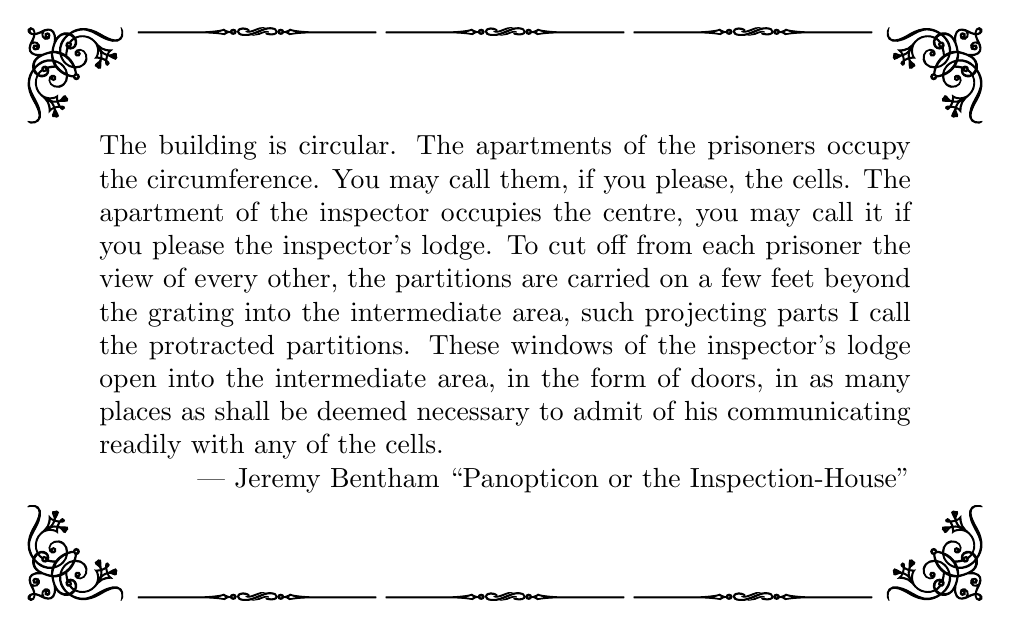
\begin{tikzpicture}[color=black,
                   transform shape,
                   every node/.style={inner sep=0pt}]
% \node[minimum size=\framesize,fill=white](vecbox){};
% \node[text width=\framesize,align=center](Text){%
%     `Then you should encode what you mean', the March Hare went on.
% \\
% `I do', Programmer hastily replied; `at least --- at least I mean what I encode --- that's the same thing, you know.'
% \\
% `Not the same thing a bit', said the Hatter.};
\node[minimum width=\framesize, minimum height=0.60 *\framesize, fill=white](vecbox){};
\node[anchor=north west] at (vecbox.north west){% 
\pgfornament[width=0.1*\framesize]{61}};
\node[anchor=north east] at (vecbox.north east){% 
\pgfornament[width=0.1*\framesize,symmetry=v]{61}};
\node[anchor=south west] at (vecbox.south west){% 
\pgfornament[width=0.1*\framesize,symmetry=h]{61}};
\node[anchor=south east] at (vecbox.south east){% 
\pgfornament[width=0.1*\framesize,symmetry=c]{61}};
\node[anchor=north] at (vecbox.north){% 
\pgfornament[width=0.25*\framesize]{88}
% \pgfornament[width=0.1*\framesize]{15}
% \pgfornament[width=0.1*\framesize]{16}
\pgfornament[width=0.25*\framesize]{88}
\pgfornament[width=0.25*\framesize]{88}
};

\node[anchor=south] at (vecbox.south){% 
% \pgfornament[width=0.25*\framesize]{88}
% \pgfornament[width=0.1*\framesize,symmetry=h]{15}
\pgfornament[width=0.25*\framesize]{88}
\pgfornament[width=0.25*\framesize]{88}
\pgfornament[width=0.25*\framesize]{88}
% \pgfornament[width=0.1*\framesize,symmetry=h]{16}
% \pgfornament[width=0.25*\framesize]{88}
};
% \node[anchor=south] at (vecbox.south){% 
% \pgfornament[width=0.6*\framesize]{46}};
% \node[anchor=north,rotate=90] at (vecbox.west){% 
% \pgfornament[width=0.6*\framesize,symmetry=h]{46}};
% \node[anchor=north,rotate=-90] at (vecbox.east){% 
% \pgfornament[width=0.6*\framesize,symmetry=h]{46}};
\node[text width=0.85\framesize,align=justify] at (vecbox.center){%
The building is circular. The apartments of the prisoners occupy the circumference. You may call them, if you please, the cells. The apartment of the inspector occupies the centre, you may call it if you please the inspector’s lodge. To cut off from each prisoner the view of every other, the partitions are carried on a few feet beyond the grating into the intermediate area, such projecting parts I call the protracted partitions. These windows of the inspector’s lodge open into the intermediate area, in the form of doors, in as many places as shall be deemed necessary to admit of his communicating readily with any of the cells. \\
\rightline{--- Jeremy Bentham ``Panopticon or the Inspection-House"}};
\end{tikzpicture}
\noindent
\begin{center}
\vspace{0.3em}

\begin{tikzpicture}[color=black,
                   transform shape,
                   every node/.style={inner sep=0pt}]
\node[minimum width=0.35\framesize, minimum height=0.05*\framesize, fill=white](vecbox){};
\node[anchor=west] at (vecbox.west){\pgfornament[width=0.08*\framesize]{16}};
\node[anchor=east] at (vecbox.east){\pgfornament[width=0.08*\framesize]{15}};
\node[inner sep=6pt] (text) at (vecbox.center){\textbf{\Large Prologue}};
\end{tikzpicture}
\vspace{-0.7em}
\end{center}
% \section{Prologue}
% \label{chap3:prologue}
\lettrine{I}{n} chapter~\ref{chap1}, we have briefly discussed the conceptual question that we would like to ask: How to intuitively understand \emph{distributed programs} using the same conceptual model as \emph{monolithic programs}? It would be beneficial to view a monolithic programs as an abstraction of distributed program, specifying the intended behaviours of the invocations and resource usage in the distributed program while abstracting away message-passing details, since it would make the process of migrating monolithic programs into a distributed setting straightforward and simplify the process of implementing a distributed system.

In this chapter, we discuss in detail our design, implementation and formalisation of a \emph{universal method invocation} (UMI) library in Rust, which supports location transparency, allowing a monolithic program to be migrated into a distributed design with minimal syntactic modification and preserves the semantics of the original program.

As a metaphorical illustration, the core idea of our attempt for conceptually modelling and understanding distributed programs as monolithic programs resembles a \emph{panopticon}, where the distributed resource management is governed by a monolithic design of Rust's ownership and borrow checking system.

\section{Introduction}
\label{chap3:introduction}
Distributed computing has extensive application in areas such as cloud computing, big data processing, web services, and blockchain systems, driving the development of modern, large-scale, and resilient software systems. Distributed systems offer many significant advantages such as scalability, fault tolerance, resource sharing, and geographical distribution. 

However, comparing to monolithic systems, distributed systems are more complex and challenging to design, implement, test and debug due to the necessity for coordination, synchronisation, and communication among distributed components. Therefore, it is a common practice to implement a system, a monolithic design is initially adopted as the implementation and deployment of a monolithic system is straightforward. Such a monolithic system needs to later be re-structured and migrated into a distributed design when it needs to be expanded into a larger scale. However, it still requires non-trivial effort to be put into the migration of a monolithic system into a distributed design.

To address these issues in the design and implementation of a distributed system as well as migrating a monolithic systems into a distributed setting, we propose our design of a UMI library in Rust. The design of the UMI library share the same underlying idea of the \emph{remote procedural call} (RPC), where a method invocation on an object can be executed on a different node within the same network, abstracting over the underlying message-passing details. Such a design allows programmers to model a distributed system focusing on \emph{what} functional features are required instead of \emph{how} these functional features are achieved via complicated network communications. Moreover, it allows applications to be migrated from a monolithic design to a distributed architecture without massive changes to source code or the needs of high-level expertise in microservices. In addition, by choosing Rust as the language for implementing the UMI framework, we are able to avoid distributed memory management hassles like distributed garbage collection while extending Rust's memory safety and data-racing free guarantees into the distributed setting.

In summary, we make following contributions:
\begin{itemize}
    \item We provide a usable \emph{Rust implementation of the UMI framework} (section~\ref{chap3:implementation}).
    \item We formalise the \emph{structural operational semantics} for a core calculus of monolithic and distributed Rust programs (section~\ref{chap3:semantics}).
    \item We prove a \emph{location transparency theorem}: With the UMI framework, when a monolithic program is deployed to multiple nodes, its semantics is preserved (section~\ref{chap3:semantics:loc-transp}).
\end{itemize}

Before stepping into the detailed discussion of the UMI library, in the next section, we will give a high-level overview of remote procedure calls and Rust.

\section{Background}
\label{chap3:background}
In distributed computing, a RPC allows a method invocation to be executed on another computer on a shared network. One application of RPC is that in an object-oriented programming paradigm, it enables a method to be invoked on an object stored on a different machine and exchange data across the network. Such a remote method invocation has the same coding as a local invocation, without the programmer explicitly coding the details for the remote interaction.
However, it is hard to support \emph{location transparency}, i.e., in most existing frameworks (e.g., Java RMI), remote invocations do not have \emph{the same semantics} as local invocations. In addition, \emph{memory management} is hard in a distributed setting, for example, distributed garbage collection is complicated.

Rust~\citep{10.5555/3271463} is high-level system programming language which \emph{guarantees memory safety} and \emph{prevents data races} by its \emph{ownership system} for memory management and \emph{borrow checker} for tracking object lifetime of all references in a program during compilation.
Since Rust has semantics that guarantees memory safety, we can extend such guarantees to the distributed computing setting, allowing us to design a RPC framework that provides safe remote method invocations.

\subsection{Remote Procedure Calls}
\label{chap3:background:rpc}
A RPC allows a computer program to request a service from another program located in a different address space, which could be on the same machine or on a different machine across a network. It is a form of client-server communication, where the requesting program is the client, and the service-providing program is the server.

The basic idea behind a RPC system is to make a remote invocation appear like a local invocation, abstracting away the underlying communication mechanisms like message passing and network protocols and simplifying distributed computing by providing a familiar programming model. When a client program calls a procedure, a RPC system will handle the task of transferring the procedure call request to the remote server, along with any necessary parameters or data. The server then executes the requested procedure and sends the results back to the client.

RPCs are particularly useful in distributed systems, where different components of an application are running on separate processes or machines. It allows these components to communicate and share resources efficiently, as if they were part of a single program. There are many common applications of RPCs. For instance, in distributed file systems, RPCs are used in distributed file systems, such as Network File System (NFS), to enable clients to access and manipulate files on remote servers transparently. In remote database access, RPCs facilitate remote access to databases, allowing client applications to execute queries and retrieve data from remote database servers. In designing web services, RPCs form the basis of many web service protocols, such as SOAP (Simple Object Access Protocol), which allows applications to communicate over the internet using XML-based messaging. In modern microservices architectures, RPCs are often used for inter-process communication between different microservices, enabling them to collaborate and share functionality. In object-oriented programming, RPCs enable objects on different machines to interact with each other, invoking methods and passing data across the network, which is the application domain that we focus on in this study.

\subsection{Rust}
\label{chap3:background:rust}
As a system programming language emphasising on safety, performance, and concurrency, Rust is designed to prevent some common programming errors, such as dereferencing null pointers and data races. Rust achieves these goals through its unique features of the ownership system, borrow checking, and lifetimes.

In Rust, each value has a variable known as its \emph{owner}. Each value can only have one owner at a time, and when the owner goes out of scope, the value is dropped, i.e., deallocated from the memory. This ownership model ensures that resources are managed correctly without the need for a garbage collector. The ownership system is fundamental to Rust and serves as the basis for its memory safety.

Rust allows functions and data structures to borrow references to values without taking ownership. This is called \emph{borrowing}. When a value is borrowed, the original owner cannot modify the value until the borrowing ends. The \emph{borrow checker} is part of Rust's compiler, which ensures that references are used safely and do not result in dangling pointers or other memory issues. Borrowing can be either mutable or immutable, where mutable references have additional constraints to prevent data races and undefined behaviours.

Lifetimes in Rust express how long references should be valid. They assist the borrow checker in ensuring that references do not outlive the data they point to. Rust uses lifetimes to prevent dangling references, which is important for memory safety. Lifetimes are explicitly stated or inferred, and they work alongside the ownership system and borrow checking to maintain memory safety and prevent data races.

With the design of the ownership system, borrow checking mechanism, and lifetimes, Rust enforces strict memory safety guarantees, i.e., means that all references point to valid memory, without requiring a garbage collector. These features also ensure that Rust programmes are free of data race by allowing only one mutable reference at a time or multiple immutable references.

\section{The Implementation of Rust UMI Library}
\label{chap3:implementation}
In the section, we present our implementation of the UMI framework as a library in Rust. With such a library, a monolithic program can be migrated into a distributed program while preserving the semantics of the original monolithic program.

\subsection{Overview}
\label{chap3:impl:overview}
To give a high-level overview of the design, in figure~\ref{chap3:impl:overview:fig}, we introduce an example of migrating a monolith program into a distributed setting, by adding the \emph{macro}s provided by the UMI library. In this example, the macro \texttt{\#[proxy\_me]} implicitly translates the declared type \texttt{A} from a \texttt{struct} that can only refer to local resources to an \texttt{enum} that can either hold local resources or be a \emph{proxy} that refers to resources held on a remote node. The initialisation method is translated by the macro \texttt{\#[umi\_init]} to create an instance of the \texttt{enum} \texttt{A} instead of an instance of the \texttt{struct} \texttt{A}. Other methods are also translated by macros to allow both an invocation on a local instance of \texttt{A} and an invocation on a proxy of \texttt{A}. To create a proxy instance, the macro \texttt{remote!(address, ...)} is used, while the syntax of the initialisation of a local instance is unchanged. The invocations of the methods defined for translated \texttt{struct} \texttt{A} take the same form of the invocation those original methods.

An invocation on a proxy is encapsulated into a serialised message and sent to the destination node of which the address is the address stored in the proxy, and then the message is deserialised and the invocation is executed at the destination. After the execution, the result of the invocation is again put into a serialised message and passed back to the calling node to be deserialised.
\begin{figure}[t]
\centering
\begin{subfigure}[t]{0.53\textwidth}
    \centering
\begin{lstlisting}[language=Rust, style=boxed]
#[proxy_me]
struct A { arg: u32 }
impl A {
  #[umi_init]
  new(arg: u32) -> A { A {arg: arg} }
  #[umi_struct_method]
  foo1(&self, a: A) { ... }
  #[umi_struct_method]
  foo2(&self, &a: A) { ...}
  #[umi_struct_method]
  foo3(&self, &mut a: A) {...} ...
}
\end{lstlisting}
    % \caption{exmaple}
\end{subfigure}
\hfill
\begin{subfigure}[t]{0.45\textwidth}
    \centering
\begin{lstlisting}[language=Rust, style=boxed]
fn main() {
  let a_remote = 
    remote!\bang!(addr, A::new(10));
  
  let a_local1 = A::new(1);
  let a_local2 = A::new(2);
  let mut a_local3 = A::new(3);
  
  a_remote.foo1(a_local1);
  a_remote.foo2(&a_local2);
  a_remote.foo3(&mut a_local3);
}
\end{lstlisting}
    % \caption{example}
\end{subfigure}
\vspace{1em}
\caption{Migrating A Monolithic Application into A Distributed Setting with UMI}
\label{chap3:impl:overview:fig}
\end{figure}

\subsection{The Design of the Translation}
\label{chap3:impl:proxy}
As we have seen in the example discussed in section~\ref{chap3:impl:overview}, the syntax of a monolithic program is translated into a distributed program by a set of macros. For a declared \texttt{struct}, the macro \texttt{\#[proxy\_me]} performs the translation:
\[
\texttt{struct}\; A\;\{\; \mathit{fields}\;\} \leadsto \texttt{enum}\; A\;\{\; \mathit{Local}\;(\;\mathit{fields}\;), \mathit{Remote}\;(\;\mathit{Address}, \mathit{ID}, \mathit{IsOwner}\;)\;\} 
\]
where the \textit{Address} is the address of the node which stores the resource of a proxy, the \textit{ID} is the identifier of a proxy's resource in the resource table that will be discussed in section~\ref{chap3:impl:resource}, and \textit{IsOwner} denotes whether a proxy is a owned reference or a borrow reference.
This macro can also translate an \texttt{enum} to allow it to represent a proxy by adding a new variant which is the proxy:
\[
\texttt{enum}\; A\;\{\; \mathit{variants}\;\} \leadsto \texttt{enum}\; A\;\{\; \mathit{variants}, \mathit{Remote}\;(\;\mathit{Address}, \mathit{ID}, \mathit{IsOwner}\;)\;\} 
\]

The translation of a \texttt{enum} does not affect its initialisation method, however, the translation of a \texttt{struct} requires its initialisation method to be changed accordingly --- instead of creating an instance of a type which is a \texttt{struct}, an instance of a \textit{Local} variant of an \texttt{enum} is created. For instance, in the example shown in figure~\ref{chap3:impl:overview:fig}, the \texttt{new(arg:u32)} method is translated by \texttt{\#[umi\_init]} into:
\begin{lstlisting}[language=Rust, style=boxed, basicstyle=\footnotesize\ttfamily]
new(arg: u32) -> A { A::Local {arg: arg} }
\end{lstlisting}

The macro \texttt{\#[umi\_struct\_method]} performs the translation of other methods of a \texttt{struct}. For instance, the method \texttt{foo1(\&self, a:A)} is translated into:
\begin{lstlisting}[language=Rust, style=boxed, basicstyle=\footnotesize\ttfamily]
fn foo1(&self, a: A) {
  match &self {
    Local(...) => { /* do something */ },
    Remote(...) => { /* remote do something */ }
}}
\end{lstlisting}
Note that within the pattern matching block for the \emph{Remote} variant, the invocation is firstly put into a message and serialised. Then the serialised message is passed to the addressed stored in the proxy, and get deserialised and executed. The result is again put into a message and get serialised. Once it is returned back to the original node, the result is extracted from the deserialised message. Such a communication process between nodes via sending and receiving serialisation/deserialisation messages is completely generated by the macro, freeing programmers from dealing with the message passing complexity.

As for a method of a translated \texttt{enum}, the macro \texttt{\#[umi\_enum\_method]} adds an additional pattern matching block for the proxy variant to the existing pattern matching.

\subsection{Resource Management}
\label{chap3:impl:resource}
To be able to use the UMI library for executing programs that access and manipulate memories of different nodes within a network, resources and computations need to be made available to and well-managed by all nodes in the network.

Firstly, a node should be able to store resources owned by different machines and deallocate those resources according to the their lifetime.
In Rust, if some resources are owned by a reference on the same node, and the reference has reached the end of its lifetime, these resources will be deallocated from the memory. With such a design, resources that are not owned by any reference on the same node are automatically deallocated. However, in our UMI library, while some resources on a node $n_1$ is not owned by any reference on the same node, they can be owned by a reference on a different node $n_2$. Although these resources do not have a local owner, the deallocation should not happen until the remote owner reaches the end of its lifetime. 
To achieve this goal, on each UMI server, we design a \emph{resource table} shown in figure~\ref{chap3:impl:tables}, which has the same lifetime of the server. We used it to identify and manage local resources involved in remote computations. Note that the ID in an entry of the table is the ID field in a corresponding proxy.
If a variable is created locally, it will be put into the table once it is passed into a remote computation. The entry will not be removed until the remote computation finishes. If a variable is created via a remote call, it will be put into table on creation and will be deallocated when its remote owner decides that it should be dropped.
\begin{figure}
\centering
\begin{tabular}{ |c|c| } 
\hline
\textbf{ID} & \textbf{Resource} \\\hline
0 & ... \\\hline
1 & ... \\\hline
... & ... \\
\hline
\end{tabular}
\quad
\begin{tabular}{ |c|c| } 
\hline
\textbf{Full Path Name} & \textbf{Type Information} \\\hline
\texttt{A::new} & \texttt{u32}, \texttt{A} \\\hline
\texttt{A::foo1} &  (\texttt{\&A}, \texttt{A}), \texttt{()} \\\hline
... & ... \\
\hline
\end{tabular}
\caption{A resource table (L) and a method registration table (R)}
\label{chap3:impl:tables}
\end{figure}

Secondly, we need to make all nodes be aware of all methods that can be invoked on a proxy in order to make computations available on all nodes. To achieve this goal, we register all methods that are available for remote invocations in a \emph{method registration table} shown in figure~\ref{chap3:impl:tables} by a \texttt{register!(name, arg\_types, return\_type)} macro. The method registration table holds the full path name, argument types, and return type of methods. When a serialised invocation message, which takes the form of a plain string, received by a node, the method to be invoked is deserialised and reconstructed according to the type information recorded in the registration table.

\subsection{Passing Remote Invocations via Messages}
\label{impl:message}
As briefly discussed in section~\ref{chap3:impl:overview} and section~\ref{chap3:impl:resource}, remote invocations and results of executions are implicitly communicated via serialised and deserialised messages among nodes. We make use of the Serde~\citep{serde} framework to serialise and deserialise these messages and Rust data structures.

There are different types of messages for passing remote invocations. For instance, a remote invocation sent to an receiving node is represented as an invocation message which taking the form of \texttt{Message::Invoke(fname, variables, invoke\_op)}, where \texttt{fname} is the full path name of the method, each variable is annotated with its ownership information (owned or immutably/mutably borrowed), and \texttt{invoke\_op} specifies the ownership information of the return value. The result of the execution of a remote invocation is passed back to the calling node via a return message taking the form of \texttt{Message::Return(return\_var)}, where the \texttt{return\_var} is also annotated with its ownership information. Another important type of messages is the deallocation message which takes the form of \texttt{Message::Drop(id)}, where the \texttt{id} corresponds to an entry key in the resource table shown in figure~\ref{chap3:impl:tables}. Such a message instructs some remotely owned resources to be deallocated.

\subsection{Extending Borrow Checking into Distributed Settings}
\label{chap3:impl:borrow}
To execute a deserialised remote method invocation on the node which receives the invocation, the first step is to gather serialised data as well as the ownership information of each variable involved in the method. In this step, we do not perform any reconstruction of these variables, instead, variables are simply prepared in an appropriate format that can be reconstructed during the execution of the method. The implementation of this step is shown in listing~\ref{chap3:impl:lst:invoke}.

A serialised variable has a label indicating that if it is a piece of data copied or moved from the caller (\texttt{OwnedLocal}), a remote reference owned by the caller (\texttt{OwnedRemote}), a remote reference immutably borrowed by the caller (\texttt{RefRemote}), or a remote reference mutably borrowed by the caller (\texttt{MutRefRemote}). 

If a variable is serialised data, which is copied or moved from the caller, it will be kept as serialised, since the deserialisation and reconstruction process will happen during the invocation of the method. 
If a variable is a proxy which is located at the receiver, then it will be obtained from the resource table shown in figure~\ref{chap3:impl:tables}. According to its ownership information, if it is moved, then the corresponding entry will be removed from the resource table. 
If it is immutably borrowed, then the corresponding entry will be immutably borrowed from the table. If it is mutably borrowed, then the corresponding entry will be mutably borrowed from the table and updated after the execution. 
If an argument is a proxy that is not located at the caller, then the proxy will be passed into the method without any additional modification.

\begin{lstlisting}[language=Rust, style=boxed, basicstyle=\footnotesize\ttfamily, caption={Gathering variables from an invocation message}, label=chap3:impl:lst:invoke]
Message::Invoke(fname, variables, invoke_op) => {
  let mut arguments: Vec<Argument> = Vec::new();
  for v in &variables {
    match v {
      Variable::OwnedLocal(s) => 
        { arguments.push(Argument::Serialised(s.clone())); },
      Variable::OwnedRemote(serialise_remote, addr, id) => {
        if addr == &local_address {
          let (owned, is_ref) = mvtable.remove(id).unwrap().into_inner();
          let arg_ref = Argument::Owned(owned);
          arguments.push(arg_ref);
        } else { 
          arguments.push(
            Argument::Serialised(serialise_remote.to_string())); }
      },
      Variable::RefRemote(serialise_remote, addr, id) => {
        if addr == &local_address {
          let borrow = mvtable.get(id).unwrap().borrow();
          let ptr: *const (Box<dyn Any + Send + Sync>, bool) = &*borrow;
          unsafe {
            let back: &(Box<dyn Any + Send + Sync>, bool) 
              = ptr.as_ref().unwrap();
            let arg_ref = Argument::Ref(&back.0, back.1);
            arguments.push(arg_ref); }
        } else { 
          arguments.push(
            Argument::RemoteRef(serialise_remote.to_string())); }
      },
      Variable::MutRefRemote(serialise_remote, addr, id) => {
        if addr == &local_address {
          let mut borrow_mut = mvtable.get(id).unwrap().borrow_mut();
          let ptr: *mut (Box<dyn Any + Send + Sync>, bool)
            = &mut *borrow_mut;
          unsafe {
            let back: &mut (Box<dyn Any + Send + Sync>, bool) 
              = ptr.as_mut().unwrap();
            let arg_ref = Argument::MutRef(&mut back.0, back.1);
            arguments.push(arg_ref); }
        } else { 
          arguments.push(Argument::RemoteMutRef(serialise_remote.clone())); 
        }
  }}}
  ...
}
\end{lstlisting}

Once the information of all variables are gathered and processed, the invocation will be executed and the result will then be sent back to the caller. The implementation of the execution of this invocation is shown in listing~\ref{chap3:impl:lst:exec-return}. The method information, mainly ownership and type information of the arguments, and return value of a method are retrieved from the registration table shown in figure~\ref{chap3:impl:tables}. During the execution of the method via \texttt{f.call(arguments)}, serialised arguments and boxed argument entries retrieved from the resource table are reconstructed according to the registered type information.

The result of an execution is provided in two formats, serialised data and a boxed data entry. These two formats are used according to the required ownership information of the return value. If the method produces an owned result annotated with \texttt{InvokeOp::Owned}, no matter the serialised data \texttt{res} is some local resources or a proxy, it will be kept as the serialised form and sent back via a return message. If the method is an initialisation call sent by the macro \texttt{remote!(...)} annotated with \texttt{InvokeOp::Init}, the boxed entry data will be inserted into the resource table and an unique \texttt{id} will be generated. In the return message, the address of the receiver, the \texttt{id}, and the ownership status which is \texttt{true} are included for the caller to construct a proxy that owns such a data entry on the receiver. For a return value that is an immutably or mutably borrowed reference, there are two situations. If the borrowed reference is local to the receiver, the reference itself will be inserted into the resource table identified by an generated unique \texttt{id}. Such an \texttt{id} and the address of the receiver will be sent back to the caller for creating an proxy that mirrors this borrowed reference. However, if a borrowed reference is not local to the receiver, meaning it already mirrors a reference on a different node, then it will not be stored in the resource table, instead, the serialised version of it will be sent back to the caller in a return message.
\begin{lstlisting}[language=Rust, style=boxed, basicstyle=\footnotesize\ttfamily, caption={Executing an invocation and returning the result}, label=chap3:impl:lst:exec-return]
Message::Invoke(fname, variables, invoke_op) => {
  ...
  let f: &str = &*fname; 
  match lrtable.get(f) {
    Some(f) => {
      let ((res, is_local), b) = f.call(arguments);
      let res_message: Message;
      match invoke_op {
        InvokeOp::Owned => { 
          res_message = Message::Return(ReturnVar::Owned(res)); 
        },
        InvokeOp::Init => {
          let id = (SystemTime::now(), m_id_gen.next());
          // b is the resource
          mvtable.insert(id.clone(), RefCell::new((b, false)));
          res_message = 
            Message::Return(ReturnVar::OwnedInit(local_address, id, true));
        },
        InvokeOp::Ref => {
          if is_local {
            let id = (SystemTime::now(), m_id_gen.next());
            // b is a reference
            mvtable.insert(id.clone(), RefCell::new((b, true)));
            res_message =
              Message::Return(ReturnVar::RefMirror(local_address, id));
          } else { 
            res_message = Message::Return(ReturnVar::RefBorrow(res)); 
          }
        },
        InvokeOp::MutRef => {
          if is_local {
            let id = (SystemTime::now(), m_id_gen.next());
            // b is a reference
            mvtable.insert(id.clone(), RefCell::new((b, true)));
            res_message =
              Message::Return(ReturnVar::MutRefMirror(local_address, id));
          } else { 
            res_message = Message::Return(ReturnVar::MutRefBorrow(res)); 
          }
      }}
      response(stream, res_message);
    },
    None => { /* report unregistered function */ }}
},
...
\end{lstlisting}

\subsection{Extending Lifetime Management into Distributed Settings}
\label{chap3:impl:lifetime}
Recall that in section~\ref{chap3:impl:resource}, we have briefly introduced storing and deallcating remoted owned resources on a node. In this section we discuss the design and implementation of a remote deallocation in detail. 

In a monolithic Rust program, when a variable that owns some resources reaches the end of its lifetime, in most cases, out of a program's scope, the resources it owns will be automatically deallocated. We extend this feature to the distributed setting. As illustrated in listing~\ref{chap3:impl:lst:drop-eg}, when the given proxy \texttt{a\_proxy} is initialised, some resources are allocated to the receiver node with the address \texttt{addr}. Although these resources do not have an owner on the same node, they should not be deallocated until its remote owner \texttt{a\_proxy} reaches the end of its lifetime. 
\begin{lstlisting}[language=Rust, style=boxed, basicstyle=\footnotesize\ttfamily, caption={An example of a remote deallocation}, label=chap3:impl:lst:drop-eg]
// on caller
fn main() {
  ...
  // the data of a_proxy is in the table on the receiver with addr
  // but it is owned by the caller and will be deallocated
  // when its owner decides to drop it
  let a_proxy = remote!\bang!(addr, A::new(10)); 
  ...
  a_proxy.foo1(...)
} // a_proxy is out of scope, its data on the remote machine is dropped
\end{lstlisting}

For monolithic programs, the deallocation is achieved via the \texttt{drop} method in destructor trait \texttt{Drop}, which in most cases is automatically implemented for Rust types. We extend this \texttt{drop} method to handle the deallocation of remotely owned resources. The implementation is shown in listing~\ref{chap3:impl:lst:drop}.
When a proxy that owns some resources on a node reaches the end of its lifetime, a serialised deallocation message is automatically sent to the node that holds these resources. 
\begin{lstlisting}[language=Rust, style=boxed, basicstyle=\footnotesize\ttfamily, caption={The implementation of a remote deallocation}, label=chap3:impl:lst:drop]
...
impl Drop for #name {
  fn drop(&mut self) {
    match self {
      Self::Remote(addr, id, is_owner) => {
        if is_owner.load(Ordering::Relaxed) {
          let msg = Message::Drop(*id);
          send(*addr, msg).unwrap(); }},
      _ => {}
}}}
...
\end{lstlisting}
As shown below, once a deallocation message is received by the targeted receiver, the entry with the corresponding \texttt{id} will be removed from the resource table (i.e., the \texttt{mvtable} in the listing). 
\begin{lstlisting}[language=Rust, style=boxed, basicstyle=\footnotesize\ttfamily]
Message::Drop(id) => { mvtable.remove(&id); }
\end{lstlisting}

After presenting the design and implementation of the UMI library, in the next chapter, we discuss the formalisation of core concepts of the UMI library base on formalised operational semantics of a core language of Rust, and sketch a proof of the location transparency theorem stating that using the UMI framework, the translation of a monolithic program into a distributed program preserves the semantics of the original program.

\section{The Operational Semantics}
\label{chap3:semantics}
We first provide a small-step operational semantics of a core language of Rust based on \citet{10.1145/3443420}'s FR, which captures the core features of Rust including copy- and move-semantics, owned and immutably/mutably borrowed references, and lexical lifetimes. We then present dFR, which extends FR to include distributed features of the UMI framework such as remote copy- and move-semantics as well as remote references. We intend to show that such an extension preserves the semantics of FR, therefore the type safety claims of FR is preserved by dFR.

\subsection{The Revised Syntax and Semantics of FR}
\label{chap3:semantics:fr}
We present the revised syntax of FR in figure~\ref{chap3:syntax:r-syntax-fig}. Note that $\&w$ and $\&\texttt{mut}\;w$ represent immutable and mutable borrowing, $\mathscr{l}^\bullet$ and $\mathscr{l}^\circ$ are owned and borrowed references where $\mathscr{l}$ represents a location in a program state. In addition, different from the original FR and Rust which do not have explicit syntax for move, we use $\#w$ to express move explicitly.

% Note that the $k$ in the block represents the lifetime.
\begin{figure}
\begin{alignat*}{3}
    \text{Term} \quad t \ \metaDeff \quad &\texttt{let mut}\;x = t;t &\text{declaration}\\
    \cmid \quad &w \metaDef t &\text{assignment}\\
    \cmid \quad &t;t &\text{sequence}\\
    \cmid \quad &\texttt{()} &\text{unit}\\
    \cmid \quad &\{t\} &\text{block}\\
    \cmid \quad &\texttt{box}\;t &\text{heap allocation}\\
    \cmid \quad &\&w \quad &\text{immutable borrow} \\
    \cmid \quad &\&\texttt{mut}\;w \quad &\text{mutable borrow} \\
    \cmid \quad &\#{w} \quad &\text{move} \\
    \cmid \quad &!{w} \quad &\text{copy} \\
    \cmid \quad &v \quad &\text{value} \\
    % \cmid \quad &w\\
    \text{LVal} \quad w \ \metaDeff \quad &x \quad &\text{variable} \\
    \cmid \quad &{*}w \quad &\text{dereference} \\
    \text{Value}(\mathcal{V}) \quad v \ \metaDeff \quad &\bot\\ 
    \cmid \quad &\texttt{()} \quad &\text{unit} \\
    \cmid \quad &i \quad &\text{integer} \\
    \cmid \quad &\mathscr{l}^\bullet &\text{owned reference} \\
    \cmid \quad &\mathscr{l}^\circ &\text{borrowed reference} \\
    \text{Location}\quad  \mathscr{l} \in \mathbb{A}
\end{alignat*}
\caption{The revised syntax of FR}
\label{chap3:syntax:r-syntax-fig}
\end{figure}

\begin{figure}
\begin{align*}
    &\mathcal{S}: \mathbb{A} \rightharpoonup \mathcal{V} \times \mathcal{L}\\
    &\mathcal{S} \mid \mathscr{l} \mapsto (v, m) \quad \text{where: } \mathscr{l} \in \textbf{dom}\;\mathcal{S} &\text{(update)}\\
    &\mathcal{S} \otimes \mathscr{l} \mapsto (v, m) \quad \text{where: } \mathscr{l} \notin \textbf{dom}\;\mathcal{S} &\text{(extend)}
\end{align*}
\caption{The program state}
\label{chap3:semantics:program:state}
\end{figure}

The notion of program state is introduced in figure~\ref{chap3:semantics:program:state}, which is a mapping from a location to a tuple of value and lifetime. When a value is replaced or its lifetime is expired, it will be removed from the program state.

We provide the operations of recursively removing values based on a location $\mathscr{l}$ and a lifetime $k$ from the state: 
\begin{align*}
      &\bigl(\mathcal{S}\otimes(\mathscr{l}^\bullet \mapsto (v, k))\bigr)\setminus {\mathscr{l}^\bullet} = \mathcal{S}\setminus v \\
      &\mathcal{S}\setminus v = \mathcal{S} \quad\text{(o/w)}
\end{align*}
and respectively:
\[
   \mathcal{S}\setminus k \ (\mathscr{l}) =
    \begin{cases}
      \mathcal{S}(\mathscr{l}) \quad\text{if $\mathcal{S}(\mathscr{l})=(v,k)$} \\
      \textbf{undefined}\quad\text{(o/w)}
    \end{cases}
\] % this  is not correct and I will revise it

Figure~\ref{semantics:r-reduction-fig} shows the small-step operational semantics of FR, which takes the form of a reduction $S, t \longrightarrow S', t'$, where $S$ is the program state before the evaluation of the term $t$, and $S', t'$ are the program state and the term after the evaluation.

Evaluating a copy term simply makes a copy of a value $v$ at a given location $\mathscr{l}$, without modifying the program state, whereas evaluating a move term moves a value $v$ out of a given location $\mathscr{l}$.
A heap allocation $\texttt{box}\;v$ puts the value $v$ into a fresh location $\mathscr{l}$ and gives it the global lifetime $\top$, which outlives all other lifetimes. The rule for evaluating a borrow term produces a borrowed reference of the give location $\mathscr{l}$.
Assignment places a given value $v'$ in the location $\mathscr{l}$, and recursively deallocates the old value $v$ from the program state.
The evaluation of a declaration allocates a given value $v$ to a fresh location $\mathscr{l}$ and substitutes latter occurrence of the declared variable $x$ with the owned reference $\mathscr{l}^\bullet$.

FR's lifetimes are based on the the lexical structure of programs. A block's lifetime $k$ based on the depth of the block. A block with deeper depth $\mathit{suc}\; k$ lives shorter than a block with depth $k$. The evaluation of a block is the evaluation of the term inside the block. At the end of the evaluation, a single value $v$ is obtained and values that have short lifetime than the current block are deallocated from the program state. The reduction rules for the evaluation of sequences are intuitive. We highlight the case for a sequence of which the first term is an owned reference. After evaluating the owned reference, it is recursively deallocated from the program state.
\begin{figure}
\begin{mathparpagebreakable}
    \inferrule*[right={(R-Copy)}]{\mathcal{S} (\mathscr{l}) = (v , m)}
    {\mathcal{S}, !{\mathscr{l}^\bullet} \longrightarrow \mathcal{S}, v}
    
    \inferrule*[right={(R-Move)}]{ }
    {\mathcal{S}\otimes \mathscr{l} \mapsto (v, m), \#\mathscr{l}^\bullet \longrightarrow \mathcal{S}\otimes \mathscr{l} \mapsto \bot, v}

    \inferrule*[right={(R-Box)}]{\mathscr{l} \notin \textbf{dom}\;\mathcal{S}}
    {\mathcal{S}, \texttt{box }v \longrightarrow \mathcal{S}\otimes \mathscr{l}\mapsto (v,\top), \mathscr{l}^\bullet}
    % \vspace{-0.3cm}
    % \\\text{Heap locations are given global lifetime $\top$ which all other lifetimes are assumes to be inside.}

    \inferrule*[right={(R-Borrow)}]{\mathscr{l} \in \textbf{dom}\; \mathcal{S}}
    {\mathcal{S}, \&[\texttt{mut}]\mathscr{l}^\bullet \longrightarrow \mathcal{S}, \mathscr{l}^\circ}

    \inferrule*[right={(R-Assign (Owned))}]{ }
    {\mathcal{S}\otimes \mathscr{l} \mapsto (v, m), \mathscr{l}^\bullet \metaDef v' \longrightarrow (\mathcal{S}\setminus v)\otimes \mathscr{l} \mapsto (v', m), \texttt{()}}
    % \\\text{Assignment should not change the lifetime of the original location}

    \inferrule*[right={(R-Assign (mut Borrowed))}]{ }
    {\mathcal{S}\otimes \mathscr{l} \mapsto (v, m), \mathscr{l}^\circ \metaDef v' \longrightarrow (\mathcal{S}\setminus v)\otimes \mathscr{l} \mapsto (v', m), \texttt{()}}

    \inferrule*[right={(R-Decl)}]{\mathscr{l} \notin \textbf{dom}\;\mathcal{S}}
    {\mathcal{S}, \texttt{let}\;\texttt{mut}\;x = v; t \stackrel k \longrightarrow \mathcal{S}\otimes \mathscr{l} \mapsto (v, k), t[x/\mathscr{l}^\bullet]}\\

    \inferrule*[right={(R-Block)}]{ }
    {\mathcal{S}, \{v\} \stackrel k\longrightarrow \mathcal{S}\setminus suc\ k, v}
    
    \inferrule*[right={(S-Block)}]
    {\mathcal{S}, t \stackrel {suc\ k}\longrightarrow \mathcal{S'}, t'}
    {\mathcal{S}, \{t\} \stackrel k\longrightarrow \mathcal{S'}, \{t'\}}
    
    \inferrule*[right={(R-Seq-OwnedRef)}]{\mathscr{l} \in \textbf{dom}\; \mathcal{S}}
    {\mathcal{S}, \mathscr{l}^\bullet; t \longrightarrow \mathcal{S}\setminus\mathscr{l}^\bullet, t} 
    
    \inferrule*[right={(R-Seq-BorrowedRef)}]{\mathscr{l} \in \textbf{dom}\; \mathcal{S}}
    {\mathcal{S}, \mathscr{l}^\circ; t \longrightarrow \mathcal{S}, t}

    \inferrule*[right={(R-Seq-Int)}]{ }
    {\mathcal{S}, i; t \longrightarrow \mathcal{S}, t}
    
    \inferrule*[right={(R-Seq-Unit)}]{ }
    {\mathcal{S}, \texttt{()}; t \longrightarrow \mathcal{S}, t}
\end{mathparpagebreakable}
    \caption{The semantics of revised FR}
    \label{semantics:r-reduction-fig}
\end{figure}
% \subsection{Evaluation Context}

An evaluation context is a term with a placeholder $\llbracket\cdot\rrbracket$. $E\llbracket t\rrbracket$ is a term obtained by replacing the placeholder with a term $t$. The evaluation context and reduction rule for the evaluation context are shown in figure~\ref{semantics:eval-context}.
\begin{figure}
    \begin{align*}
        E \metaDeff \llbracket \cdot \rrbracket \cmid E;t \cmid v; E \cmid \texttt{let mut }x=E; t \cmid \texttt{let mut }x = v; E \cmid \{E\} \cmid \texttt{box }E \cmid w = E
    \end{align*}
    \begin{mathpar}
    \inferrule*[right={(R-Context)}]{ S, t \longrightarrow S, t' }
        { S, E\llbracket t \rrbracket \longrightarrow  S', E\llbracket t' \rrbracket }
    \end{mathpar}
    \caption{Evaluation context}
    \label{semantics:eval-context}
\end{figure}

Next, we will discuss the semantics of dFR, which extends the FR with distributed computation features including remote references and values.

\subsection{The Syntax and Semantics of dFR} 
\label{chap3:semantics:dfr}
Figure~\ref{syntax:d-syntax-fig} shows the syntax of dFR, which is the syntax of FR discussed in section~\ref{chap3:semantics:fr} extended with the remote declaration $\texttt{let}\;\texttt{mut}@n\; x = t;t$, remote heap allocation $\texttt{box}\;t$, remote values $v@n$, and remote terms $t@n$. Note that $n$ is the address of a node and $\mathcal{N}$ is the set of addresses. 
% $\mathscr{l}^\bullet_{@n}$ denotes a owned reference on the node $n$. 
\begin{figure}
\begin{alignat*}{3}
    \text{Term}(T) \quad t \ \metaDeff \quad &\texttt{let mut } x = t;t &\text{declaration}\\
    \cmid \quad &\texttt{let mut}@n\; x = t;t &\text{remote declaration}\\
    \cmid \quad &w \metaDef t &\text{assignment}\\
    \cmid \quad &t;t &\text{sequence}\\
    \cmid \quad &\texttt{()} &\text{unit}\\
    \cmid \quad &\{t\} &\text{block}\\
    \cmid \quad &\texttt{box } t &\text{heap allocation}\\
    \cmid \quad &\texttt{box}@n\; t &\text{remote  heap allocation}\\
    \cmid \quad &\&w \quad &\text{immutable borrow} \\
    \cmid \quad &\&\texttt{mut } w \quad &\text{mutable borrow} \\
    \cmid \quad &\#{w} \quad &\text{move} \\
    \cmid \quad &!{w} \quad &\text{copy} \\
    \cmid \quad &v \quad &\text{value} \\
    \cmid \quad &v@n \quad &\text{remote value}\\
    \text{Remote Term} \quad t_d \metaDeff \quad &t@n\\
    \text{LVal} \quad w \ \metaDeff \quad &x \quad &\text{variable} \\
    \cmid \quad &{*}w \quad &\text{dereference} \\
    \text{Value}(\mathcal{V}) \quad v \ \metaDeff \quad &\bot\\ 
    \cmid \quad &\texttt{()} \quad &\text{unit} \\
    \cmid \quad &i \quad &\text{integer} \\
    \cmid \quad &\mathscr{l}^\bullet &\text{owned reference} \\
    \cmid \quad &\mathscr{l}^\circ &\text{borrowed reference} \\
    \text{Location}\quad  \mathscr{l} \in \mathbb{A}
    &\quad\quad\quad\quad\text{Node}\quad n \in \mathcal{N}
\end{alignat*}
\caption{The syntax of dFR}
\label{syntax:d-syntax-fig}
\end{figure}

Building upon the program state $\mathcal{S}$ for FR, in figure~\ref{d-state}, we introduce the distributed program state $\mathcal{D}$, which maps addresses of nodes to their program states. The reduction rule takes the form of $\mathcal{D}, \mathcal{C}_s \longrightarrow \mathcal{D'}, \mathcal{C}_s'$, where $\mathcal{C}_s$ and $\mathcal{C}_s'$ are configuration stacks. For each reduction, the term on the top of a configuration stack $\mathcal{C}_s$ gets evaluated. The element of the configuration stack can either be a pair of an address and a hole ($n, ?$) or a pair of an address and a term ($n, t$).
\begin{figure}
    \begin{align*}
        &\mathcal{D}: \mathcal{N} \rightharpoonup \mathcal{S}
        %&\mathit{nt} \in  \mathcal{N} \times\mathds{1} + \mathcal{N}\times T\\
        &\mathit{nt} \in  \mathcal{N} \times\mathds{1} + \mathcal{N}\times T\\
        &\mathcal{C}_s : (nt)^*
        &\mathrm{Configuration}: \mathcal{D}, \mathcal{C}_s
    \end{align*}
    \caption{Distributed program state and configuration stack}
    \label{d-state}
\end{figure}

\begin{figure}
    \begin{mathpar}
        \inferrule*[right={(Copy (s1))}]{ \mathcal{D}(n')(\mathscr{l}) = (v, m) }
        {\mathcal{D}, \mathcal{C}_s \concat (n, !\mathscr{l}^\bullet_{@n'}) \longrightarrow \mathcal{D}, \mathcal{C}_s \concat (n, ?) \concat (n', !\mathscr{l}^\bullet)}
        
        \inferrule*[right={(Copy (s2))}]{ \mathcal{D}(n')(\mathscr{l}) = (v, m)}
        {\mathcal{D}, \mathcal{C}_s \concat (n, ?) \concat (n',!\mathscr{l}^\bullet) \longrightarrow \mathcal{D}, \mathcal{C}_s \concat (n, v@n')}

        \inferrule*[right={(Move (s1))}]{ }
        {\mathcal{D} \otimes (n' \mapsto \mathcal{S}\otimes\mathscr{l} \mapsto (v, m)), \mathcal{C}_s \concat (n, \#\mathscr{l}^\bullet_{@n'}) \longrightarrow \\\mathcal{D} \otimes (n' \mapsto \mathcal{S}\otimes\mathscr{l} \mapsto (v, m)), \mathcal{C}_s \concat (n, ?) \concat (n', \#\mathscr{l}^\bullet)}

        \inferrule*[right={(Move (s2))}]{ }
        {\mathcal{D} \otimes (n' \mapsto \mathcal{S}\otimes \mathscr{l} \mapsto (v, m)), \mathcal{C}_s \concat (n, ?) \concat (n', \#\mathscr{l}^\bullet) \longrightarrow \\\mathcal{D} \otimes (n' \mapsto \mathcal{S}\otimes\mathscr{l} \mapsto \bot), \mathcal{C}_s \concat (n, v@n')}

        \inferrule*[right={(Box (s1))}]{ }
        {\mathcal{D}, \mathcal{C}_s \concat (n, (\texttt{box}@n'\;v)) \longrightarrow \mathcal{D}, \mathcal{C}_s \concat (n, ?) \concat (n', \texttt{box}\;v)}

        \inferrule*[right={(Box (s2))}]{ \mathscr{l} \notin \textbf{dom}\;\mathcal{D}(n') }
        {\mathcal{D}, \mathcal{C}_s \concat (n, ?) \concat (n', \texttt{box}\;v) \longrightarrow \mathcal{D} \mid (n' \mapsto \mathcal{D}(n')\otimes\mathscr{l}\mapsto (v, \top)), \mathcal{C}_s \concat (n, \mathscr{l}^\bullet_{@n'})} 

        \inferrule*[right={(Borrow (s1))}]{ \mathscr{l} \in \textbf{dom}\;\mathcal{D}(n') }
        {\mathcal{D}, \mathcal{C}_s \concat (n, \&[\texttt{mut}]\mathscr{l}^\bullet_{@n'}) \longrightarrow \mathcal{D}, \mathcal{C}_s \concat (n, ?) \concat (n', \&[\texttt{mut}]\mathscr{l}^\bullet)}

        \inferrule*[right={(Borrow (s2))}]{ \mathscr{l} \in \textbf{dom}\;\mathcal{D}(n') }
        {\mathcal{D}, \mathcal{C}_s \concat (n, ?) \concat (n', \&[\texttt{mut}]\mathscr{l}^\bullet) \longrightarrow \mathcal{D}, \mathcal{C}_s \concat (n, \mathscr{l}^\circ_{@n'})}
    \end{mathpar}
    \caption{The semantics of dFR (part one)}
    \label{semantics:eval-distributed-1}
\end{figure}

Utilising the distributed program state and the configuration stack, we provide the semantics of dFR in figure~\ref{semantics:eval-distributed-1} and figure~\ref{semantics:eval-distributed-2}. Note that all reduction rules for evaluating terms presented in FR are adapted into reduction rules for dFR via the rule \textsc{Local Term}. 

To evaluate copying a remotely owned reference $\mathscr{l}^\bullet_{@n'}$ on a node with address $n$, the first step shown in the rule \textsc{Copy (s1)} is to update the configuration stack by changing the $(n, !\mathscr{l}^\bullet_{@n'})$ to $(n, ?)$, and pushing a new address-term pair $(n', !\mathscr{l}^\bullet)$ to be evaluated onto the stack. It models that the computation is passed to the node $n'$, which stores the resource owned by the reference $\mathscr{l}^\bullet_{@n'}$. Then the rule \textsc{Copy (s2)} indicates that the copy term $!\mathscr{l}^\bullet$ gets evaluated on the node $n'$, and the resulting value annotated with the address $n'$ is passed back to fill in the hole. Similarly, as for the semantics of moving the value out of a remote owned reference, the first step is to replace the term on the node $n$ with a hole, and pass the copy term to the node $n'$ to evaluate. The resulting value $v$ annotated with the address $n'$ is passed back to the node $n$ at the end of the evaluation to fill in the hole, and the value of the location $\mathscr{l}$ at the program state of the node $n'$ is replaced by $\bot$, indicating that the value is moved out of the location $\mathscr{l}$ at the node $n'$.

The rules \textsc{Box (s1)} and \textsc{Box (s2)} show the evaluation of a remote heap allocation $\texttt{box}@n'\;v$ on the node $n$. Firstly, the heap allocation is passed to the node $n'$ to be evaluated, and a hole on the node $n$ is created and pushed onto the configuration stack. The value $v$ is stored in a fresh location $\mathscr{l}$ at the program state of the node $n'$ and assigned with the lifetime $\top$ since it is a heap allocation, hence a owned reference $\mathscr{l}^\bullet$ is created in the node $n'$. Such a owned reference is then passed back to the node $n$ allowing the node $n$ to own the location $\mathscr{l}$ created by the heap allocation on the node $n'$. At the end of the evaluation, as shown in the rule \textsc{Box (s2)}, on the top of the configuration stack, the hole create on the node $n$ is filled by the owned remote reference $\mathscr{l}^\bullet_{@n'}$

\begin{figure}
    \begin{mathpar}
        \inferrule*[right={(Assign (s1))}]{ }
        {\mathcal{D} \otimes (n' \mapsto \mathcal{S}\otimes \mathscr{l} \mapsto (v, m)), \mathcal{C}_s \concat (n, \mathscr{l}_{@n'}^\bullet \metaDef v') \longrightarrow \\ \mathcal{D}\otimes (n' \mapsto \mathcal{S}\otimes \mathscr{l} \mapsto (v, m)), \mathcal{C}_s \concat (n, ?) \concat (n', \mathscr{l}^\bullet \metaDef v')}

        \inferrule*[right={(Assign (s2))}]{ }
        {\mathcal{D}\otimes (n' \mapsto \mathcal{S}\otimes \mathscr{l} \mapsto (v, m)), \mathcal{C}_s \concat (n, ?) \concat (n', \mathscr{l}^\bullet \metaDef v') \longrightarrow \\ \mathcal{D}\otimes (n' \mapsto \mathcal{S} \setminus v \otimes \mathscr{l} \mapsto (v', m)), \mathcal{C}_s \concat (n, \texttt{()})}

        \inferrule*[right={(Decl (s1))}]{ }
        {\mathcal{D}, \mathcal{C}_s \concat (n, \texttt{let mut}@n'\; x = v; t) \longrightarrow\\ \mathcal{D}, \mathcal{C}_s \concat (n, t[x/?]) \concat (n', \texttt{let mut } x = v; x)}

        \inferrule*[right={(Decl (s2))}]{ \mathscr{l} \notin \textbf{dom}\;\mathcal{D}(n') }
        {\mathcal{D}, \mathcal{C}_s \concat (n, t[x/?]) \concat (n', \texttt{let mut } x = v; x) \longrightarrow \\\mathcal{D} \otimes (n' \mapsto \mathcal{S}\otimes \mathscr{l} \mapsto (v, k)), \mathcal{C}_s \concat (n, t[x/ \mathscr{l}^\bullet_{@n'}])}

        \inferrule*[right={(Local Terms)}]{ \mathcal{S}, t \longrightarrow \mathcal{S}', t'}
        {\mathcal{D}\otimes(n \mapsto \mathcal{S}), \mathcal{C}_s \concat (n, t) \longrightarrow \mathcal{D}\otimes(n \mapsto \mathcal{S}'), \mathcal{C}_s \concat (n, t')}

        \inferrule*[right={(Remote Terms)}]{\mathcal{D}\otimes(n \mapsto \mathcal{S}), \mathcal{C}_s \concat (n, t) \longrightarrow \mathcal{D}\otimes(n \mapsto \mathcal{S}'), \mathcal{C}_s \concat (n, t')}
        {\mathcal{D}\otimes(n' \mapsto \mathcal{S}), \mathcal{C}_s \concat (n, t@n') \longrightarrow \mathcal{D}\otimes(n' \mapsto \mathcal{S}'), \mathcal{C}_s \concat (n, t@n')}
    \end{mathpar}
    \caption{The semantics of dFR (part two)}
    \label{semantics:eval-distributed-2}
\end{figure}

The rules \textsc{Borrow (s1)} and \textsc{Borrow (s2)} show the evaluation of immutable and mutable borrow terms. On a given node $n$, to borrow a remotely owned reference from a different node $n'$, firstly a hole is again created and pushed waiting for a term to be passed back, and the borrow term $\&[\texttt{mut}]\mathscr{l}^\bullet_{@n'}$ is passed to the node $n'$ to be evaluated. After it being evaluated on the node $n'$, the resulting remotely borrowed reference $\mathscr{l}^\circ_{@n'}$ is passed back to the node $n$ filling the hole on the configuration stack.

A remote assignment $\mathscr{l}^\bullet_{@n'} \metaDef v'$ on the node $n$ assigns a new value $v'$ to its remotely owned reference on the node $n'$. It modifies the program state on the node $n'$ by recursively deallocates the old value $v$ which is stored in the location $\mathscr{l}$ and assigns the location $\mathscr{l}$ with the new value $v'$. The evaluation of a remote declaration is more complicated. The first step leaves a hole for the substitution of the declared variable $x$. Once a fresh location $\mathscr{l}$ on the node $n'$ is allocated with the value $v$, the owned reference $\mathscr{l}^\bullet$ will then be passed back to the node $n$ and all occurrences of the declared variable will be substituted with the remote owned reference $\mathscr{l}_{@n'}^\bullet$.

\subsection{Type Safety of the Extension}
\label{chap3:semantics:loc-transp}
By extending FR into dFR, the type system and static checking of the validity of owning, immutably borrowing and mutably borrowing resources remain unchanged. This is because with our design, if we flatten a distributed program in a single node program, the flattened result of the execution of the distributed program should be the same as the result of the execution of the flattened single node program. Formally, we state this property of our distributed extension in theorem~\ref{chap3:thm:loc-transp}.

Note that the reverse direction of the theorem does not hold. Since to extend a given single node program into a distributed program by allocating the program state on arbitrary nodes and making the term involved in the execution containing remote components that live on arbitrary nodes may not lead to constructing a distributed program that can be successfully executed. However, because our goal is to show that the distributed program preserves the same behaviour as if it is a single node program, having only one direction in the theorem is sufficient.

\begin{theorem}[Location Transparency]
For any term $t$, given an initial distributed program state $\mathcal{D}$ and an initial single node program state $\mathcal{S}$, where the flattened distributed program state equals to the single node program state, if a distributed execution of a term $t$ that may be a remote term or contain remote component with the distributed program state $\mathcal{D}$ results in a distributed program state $\mathcal{D}'$ and a value $v$ which can be either remote or local, then the execution of the flattened term $t$ with the single node program state $\mathcal{S}$ will gives a state $\mathcal{S}'$ and value $v'$, where the flattened resulting distributed program state $|\mathcal{D}'|$ equals to the $S'$ and the flattened value $v$ equals to $v'$. Note that we make locations on all nodes distinct to simplify the proof.
\begin{align*}
    % &\forall t \in \Pi_{\mathit{ref}}.\; \phi_\mathcal{D}, [t] \longrightarrow \mathcal{D}, [v] \iff \phi_\mathcal{S},  t|_@ \longrightarrow \mathcal{S}, v' \land \mathcal{S} = |\mathcal{D}| \land v' = v\\
    &\forall t \in \mathrm{Term}.\; \mathcal{D}, [(n, t)] \longrightarrow \mathcal{D'}, [(n, v)] \land |\mathcal{D}| = \mathcal{S}  \Rightarrow \mathcal{S},  t|_@ \longrightarrow \mathcal{S'}, v' \land |\mathcal{D}'| = \mathcal{S}' \land v|_@ = v'\\
    &\mathrm{where:}\\
    &|\mathcal{D}| = \bigcup_{\forall n \in \textbf{dom} \mathcal{D}} \mathcal{D}(n)\\
    &\texttt{let mut }@n\; x=t; t|_@ =  \texttt{let mut } x=t; t\\
    &\texttt{box}@n\; t |_@ = \texttt{box }t\\
    &v@n|_@ = v\\
    &t_d|_@ = t |_@
\end{align*}
\label{chap3:thm:loc-transp}
\end{theorem}
Since a term $t$ is always a closed term, we prove the theorem~\ref{thm:loc-transp} by structural induction on the term $t$.
\begin{proof}[Case copy]
    \begin{align*}
    &\text{We assume:}\\
    &\mathcal{D} = \mathcal{D}_0 \otimes (n' \mapsto (l\mapsto (v, m)))\quad
    \mathcal{S} = \mathcal{S}_0 \otimes (\mathscr{l} \mapsto (v, m))\\
    &|\mathcal{D}| = \mathcal{S}\\
    &\text{The distributed execution gives:}\\
    &\mathcal{D}_0 \otimes (n' \mapsto (\mathscr{l} \mapsto (v,m))) , [(n, !\mathscr{l}^\bullet_{@n'})] \longrightarrow \mathcal{D}_0 \otimes (n' \mapsto (\mathscr{l} \mapsto (v, m))), [(n, v@n')]\\
    &\text{The monolithic execution gives:}\\
    &\mathcal{S}_0 \otimes (\mathscr{l} \mapsto (v, m)), !\mathscr{l}^\bullet_{@n'}|_@ \longrightarrow \mathcal{S}_0 \otimes (\mathscr{l} \mapsto (v, m)), v\\
    &\text{To conclude, after executions:}\\
    &\mathcal{D}' = \mathcal{D}_0 \otimes (n' \mapsto (\mathscr{l} \mapsto (v, m))) \quad 
    \mathcal{S}' = \mathcal{S}_0 \otimes (\mathscr{l} \mapsto (v, m))\\
    &|\mathcal{D}'| = \mathcal{S}' \quad \text{and} \quad v@n'|_@ = v
    \end{align*}
\end{proof}
\begin{proof}[Case move]
    \begin{align*}
    &\text{We assume:}\\
    &\mathcal{D} = \mathcal{D}_0 \otimes (n' \mapsto (l\mapsto (v, m)))\quad
    \mathcal{S} = \mathcal{S}_0 \otimes (\mathscr{l} \mapsto (v, m))\\
    &|\mathcal{D}| = \mathcal{S}\\
    &\text{The distributed execution gives:}\\
    &\mathcal{D}_0 \otimes (n' \mapsto (\mathscr{l} \mapsto (v,m))) , [(n, \#\mathscr{l}^\bullet_{@n'})] \longrightarrow \mathcal{D}_0 \otimes (n' \mapsto (\mathscr{l} \mapsto \bot), [(n, v@n')]\\
    &\text{The monolithic execution gives:}\\
    &\mathcal{S}_0 \otimes (\mathscr{l} \mapsto (v, m)), \#\mathscr{l}^\bullet_{@n'}|_@ \longrightarrow \mathcal{S}_0 \otimes (\mathscr{l} \mapsto \bot), v\\
    &\text{To conclude, after executions:}\\
    &\mathcal{D}' = \mathcal{D}_0 \otimes (n' \mapsto (\mathscr{l} \mapsto \bot)) \quad 
    \mathcal{S}' = \mathcal{S}_0 \otimes (\mathscr{l} \mapsto \bot)\\
    &|\mathcal{D}'| = |\mathcal{D}_0| \otimes (\mathscr{l} \mapsto \bot) = \mathcal{S}_0 \otimes (\mathscr{l} \mapsto \bot) = \mathcal{S}' \quad \text{and} \quad v@n'|_@ = v
    \end{align*}
\end{proof}
\begin{proof}[Case box]
    \begin{align*}
    &\text{We assume:}\\
    &|\mathcal{D}| = \mathcal{S} \quad \mathscr{l} \notin \textbf{dom}\; \mathcal{D}(n') \quad \mathscr{l} \notin \textbf{dom}\; \mathcal{S}\\
    &\text{The execution of the distributed program gives:}\\
    &\mathcal{D}, [(n, \texttt{box}@n'\;v)] \longrightarrow \mathcal{D} \mid (n' \mapsto \mathcal{D}(n')\otimes(\mathscr{l} \mapsto (v, \top))), [(n, \mathscr{l}^\bullet_{@n'})]\\
    &\text{The execution of the monolithic program gives:}\\
    &\mathcal{S}, (\texttt{box}@n'\;v)|_@ \longrightarrow \mathcal{S} \otimes (\mathscr{l} \mapsto (v, \top)), \mathscr{l}^\bullet\\
    &\text{To conclude, after executions:}\\
    &\mathcal{D}' = \mathcal{D}(n')\otimes(\mathscr{l} \mapsto (v, \top)) \quad 
    \mathcal{S}' =  \mathcal{S} \otimes (\mathscr{l} \mapsto (v, \top))\\
    &|\mathcal{D}'| = |\mathcal{D}| \otimes (\mathscr{l} \mapsto (v, \top)) = \mathcal{S} \otimes (\mathscr{l} \mapsto (v, \top))= \mathcal{S}' \quad \text{and} \quad \mathscr{l}^\bullet_{@n'}|_@ = \mathscr{l}^\bullet
    \end{align*}
\end{proof}
\begin{proof}[Case borrow]
    \begin{align*}
    &\text{We assume:}\\
    &|\mathcal{D}| = \mathcal{S} \quad \mathscr{l} \in \textbf{dom}\; \mathcal{D}(n') \quad \mathscr{l} \in \textbf{dom}\; \mathcal{S}\\
    &\text{The execution of the distributed program gives:}\\
    &\mathcal{D}, [(n, \&[\texttt{mut}]\mathscr{l}^\bullet_{@n'})] \longrightarrow \mathcal{D} [(n, \mathscr{l}^\circ_{@n'})]\\
    &\text{The execution of the monolithic program gives:}\\
    &\mathcal{S}, (\&[\texttt{mut}]\mathscr{l}^\bullet_{@n'})|_@ \longrightarrow \mathcal{S}, \mathscr{l}^\circ\\
    &\text{To conclude, after executions:}\\
    &\mathcal{D}' = \mathcal{D}\quad 
    \mathcal{S}' =  \mathcal{S}\quad
    |\mathcal{D}'| = \mathcal{S}' \quad \text{and} \quad \mathscr{l}^\circ_{@n'}|_@ = \mathscr{l}^\circ
    \end{align*}
\end{proof}
\begin{proof}[Case assign]
    \begin{align*}
    &\text{We assume:}\\
    &\mathcal{D} = \mathcal{D}_0 \otimes (n' \mapsto (l\mapsto (v, m)))\quad
    \mathcal{S} = \mathcal{S}_0 \otimes (\mathscr{l} \mapsto (v, m))\\
    &|\mathcal{D}| = \mathcal{S}\\
    &\text{The execution of the distributed program gives:}\\
    &\mathcal{D}_0 \otimes (n' \mapsto (\mathscr{l} \mapsto (v,m))) , [(n, \mathscr{l}^\bullet_{@n'} \metaDef v')] \longrightarrow \mathcal{D}_0 \otimes (n' \mapsto (\mathscr{l} \mapsto (v',m))), [(n, \texttt{()}@n')]\\
    &\text{The execution of the monolithic program gives:}\\
    &\mathcal{S}_0 \otimes (\mathscr{l} \mapsto (v, m)), (\mathscr{l}^\bullet_{@n'} \metaDef v')|_@ \longrightarrow \mathcal{S}_0 \otimes (\mathscr{l} \mapsto (v', m)), \texttt{()}\\
    &\text{To conclude, after executions:}\\
    &\mathcal{D}' = \mathcal{D}_0 \otimes (n' \mapsto (\mathscr{l} \mapsto (v',m))) \quad 
    \mathcal{S}' = \mathcal{S}_0 \otimes (\mathscr{l} \mapsto (v', m))\\
    &|\mathcal{D}'| = |\mathcal{D}_0| \otimes (\mathscr{l} \mapsto (v', m)) = \mathcal{S}_0 \otimes (\mathscr{l} \mapsto (v', m)) = \mathcal{S}' \quad \text{and} \quad \texttt{()}@n'|_@ = \texttt{()}
    \end{align*}
\end{proof}
\begin{proof}[Case decl]
    \begin{align*}
    &\text{We assume:}\\
    &|\mathcal{D}| = \mathcal{S} \quad \mathscr{l} \notin \textbf{dom}\; \mathcal{D}(n') \quad \mathscr{l} \notin \textbf{dom}\; \mathcal{S}\\
    &\text{The execution of the distributed program gives:}\\
    &\mathcal{D}, [(n, \texttt{let mut}@n' x = v;t)] \longrightarrow \mathcal{D} \mid (n' \mapsto \mathcal{D}(n')\otimes(\mathscr{l} \mapsto (v, k))), [(n, t[x/\mathscr{l}^\bullet_{@n'}])]\\
    &\text{The execution of the monolithic program gives:}\\
    &\mathcal{S}, (\texttt{let mut}@n' x = v;t)|_@ \longrightarrow \mathcal{S} \otimes (\mathscr{l} \mapsto (v, k)), t[x/\mathscr{l}^\bullet]\\
    &\text{To conclude, after executions:}\\
    &\mathcal{D}' = \mathcal{D} \mid (n' \mapsto \mathcal{D}(n')\otimes(\mathscr{l} \mapsto (v, k))) \quad 
    \mathcal{S}' = \mathcal{S} \otimes (\mathscr{l} \mapsto (v, k))\\
    &|\mathcal{D}'| = |\mathcal{D}| \otimes (\mathscr{l} \mapsto (v, k)) = \mathcal{S} \otimes (\mathscr{l} \mapsto (v, k)) = \mathcal{S}' \quad \text{and} \quad t[x/\mathscr{l}^\bullet]|_@ = t[x/(\mathscr{l}^\bullet)|_@] = t[x/\mathscr{l}^\bullet]
    \end{align*}
\end{proof}
The proofs for location transparency of the distributed and monolithic executions of local terms and remote terms should then be trivial.

\section{Related Work}
\label{chap3:related-work}

\section{Conclusion}
\label{chap3:conclusion}

\noindent
\begin{center}
\vspace{0.3em}

\begin{tikzpicture}[color=black,
                   transform shape,
                   every node/.style={inner sep=0pt}]
\node[minimum width=0.35\framesize, minimum height=0.05*\framesize, fill=white](vecbox){};
\node[anchor=west] at (vecbox.west){\pgfornament[width=0.08*\framesize]{16}};
\node[anchor=east] at (vecbox.east){\pgfornament[width=0.08*\framesize]{15}};
\node[inner sep=6pt] (text) at (vecbox.center){\textbf{\Large Epilogue}};
\end{tikzpicture}
\vspace{-0.7em}
\end{center}
\Chapter{Capturing A Shape-Shifter: The Semantic Process}{A Formal Foundation for Strategic Rewriting}
\label{chap4}

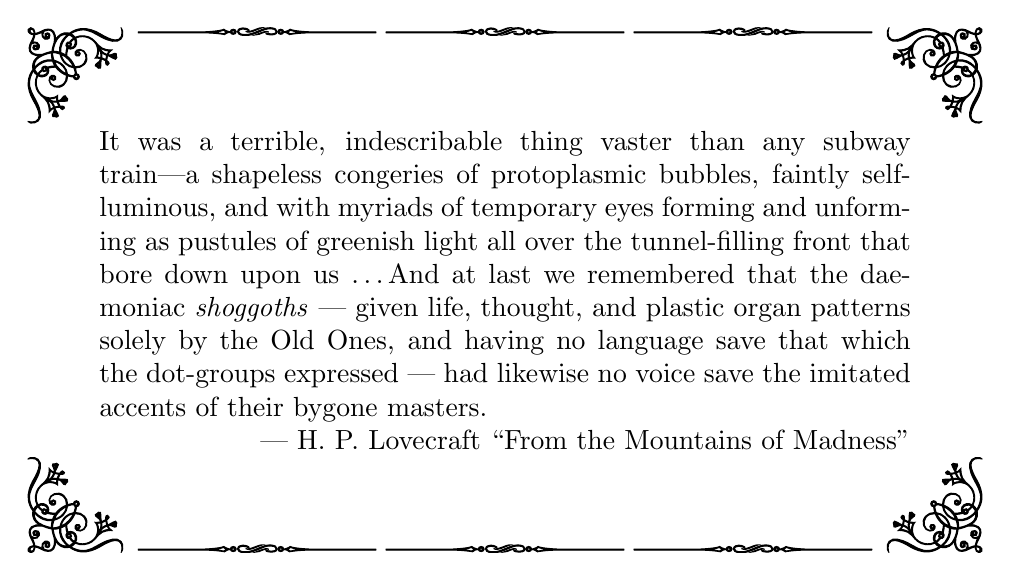
\begin{tikzpicture}[color=black,
                   transform shape,
                   every node/.style={inner sep=0pt}]
% \node[minimum size=\framesize,fill=white](vecbox){};
% \node[text width=\framesize,align=center](Text){%
%     `Then you should encode what you mean', the March Hare went on.
% \\
% `I do', Programmer hastily replied; `at least --- at least I mean what I encode --- that's the same thing, you know.'
% \\
% `Not the same thing a bit', said the Hatter.};
\node[minimum width=\framesize, minimum height=0.55 *\framesize, fill=white](vecbox){};
\node[anchor=north west] at (vecbox.north west){% 
\pgfornament[width=0.1*\framesize]{61}};
\node[anchor=north east] at (vecbox.north east){% 
\pgfornament[width=0.1*\framesize,symmetry=v]{61}};
\node[anchor=south west] at (vecbox.south west){% 
\pgfornament[width=0.1*\framesize,symmetry=h]{61}};
\node[anchor=south east] at (vecbox.south east){% 
\pgfornament[width=0.1*\framesize,symmetry=c]{61}};
\node[anchor=north] at (vecbox.north){% 
\pgfornament[width=0.25*\framesize]{88}
% \pgfornament[width=0.1*\framesize]{15}
% \pgfornament[width=0.1*\framesize]{16}
\pgfornament[width=0.25*\framesize]{88}
\pgfornament[width=0.25*\framesize]{88}
};

\node[anchor=south] at (vecbox.south){% 
% \pgfornament[width=0.25*\framesize]{88}
% \pgfornament[width=0.1*\framesize,symmetry=h]{15}
\pgfornament[width=0.25*\framesize]{88}
\pgfornament[width=0.25*\framesize]{88}
\pgfornament[width=0.25*\framesize]{88}
% \pgfornament[width=0.1*\framesize,symmetry=h]{16}
% \pgfornament[width=0.25*\framesize]{88}
};
% \node[anchor=south] at (vecbox.south){% 
% \pgfornament[width=0.6*\framesize]{46}};
% \node[anchor=north,rotate=90] at (vecbox.west){% 
% \pgfornament[width=0.6*\framesize,symmetry=h]{46}};
% \node[anchor=north,rotate=-90] at (vecbox.east){% 
% \pgfornament[width=0.6*\framesize,symmetry=h]{46}};
\node[text width=0.85\framesize,align=justify] at (vecbox.center){%
It was a terrible, indescribable thing vaster than any subway train—a shapeless congeries of protoplasmic bubbles, faintly self-luminous, and with myriads of temporary eyes forming and unforming as pustules of greenish light all over the tunnel-filling front that bore down upon us \dots 
%crushing the frantic penguins and slithering over the glistening floor that it and its kind had swept so evilly free of all litter. Still came that eldritch, mocking cry --- \textit{``Tekeli-li! Tekeli-li!"} 
And at last we remembered that the daemoniac \emph{shoggoths} --- given life, thought, and plastic organ patterns solely by the Old Ones, and having no language save that which the dot-groups expressed --- had likewise no voice save the imitated accents of their bygone masters.\\
\rightline{--- H. P. Lovecraft ``From the Mountains of Madness"}};
% \node[text width=0.85\framesize,align=right] at (vecbox.south){%
%    --- \emph{Altered} Alice's Adventures in Wonderland};
\end{tikzpicture}
\noindent
\begin{center}
\vspace{0.3em}

\begin{tikzpicture}[color=black,
                   transform shape,
                   every node/.style={inner sep=0pt}]
\node[minimum width=0.35\framesize, minimum height=0.05*\framesize, fill=white](vecbox){};
\node[anchor=west] at (vecbox.west){\pgfornament[width=0.08*\framesize]{16}};
\node[anchor=east] at (vecbox.east){\pgfornament[width=0.08*\framesize]{15}};
\node[inner sep=6pt] (text) at (vecbox.center){\textbf{\Large Prologue}};
\end{tikzpicture}
\vspace{-0.3em}
\end{center}
% \section{Prologue}
% \label{chap4:prologue}
\lettrine{A}{s} illustrated in the quotation, \emph{Shoggoth} is a Lovecraftian \emph{shape-shifting monster}, making the sound ``Tekeli-li, Tekeli-li" which can no longer be understood by anyone. In this chapter, we thoroughly discuss about a foundational study of a domain specific programming language --- a strategic rewriting language for \emph{syntactic transformations}, which is previously lack of formal treatment. By making a metaphorical connection, we have named study Shoggoth and published it under the title \emph{Shoggoth: A Formal Foundation for Strategic Rewriting}. 

In chapter~\ref{chap1}, we have briefly discussed that conceptually it is intriguing to explore the relationship between syntax and semantics within the context of strategic rewriting. Since term rewriting, as syntactic transformations, encodes the semantics of some programs, and the compositions of each individual term rewriting step form strategies, of which the straightforward syntax is given by a strategic rewriting language, whose semantics featuring non-termination and non-deterministic executions is complicated and worth studying to all us to formally understand and reason about the composition of these rewrites.

In this chapter, we utilise three formal semantics models of programming languages, namely, denotational semantics, big-step operational semantics, and axiomatic semantics, to analyse a core calculus of a set of strategic rewriting languages, and discussed how these models relate to each other.

\section{Introduction}
\label{chap4:introduction}
Strategic rewriting allows programmers to compose rewrite rules and control their application.
Dedicated strategy languages, such as Stratego~\citep{DBLP:conf/icfp/VisserBT98,10.1007/3-540-45127-7_27} and more recently Elevate~\citep{DBLP:journals/cacm/HagedornLKQGS23,DBLP:journals/pacmpl/HagedornLKQGS20}, provide combinators for composing rewrite rules into larger strategies, as well as traversals to describe the location at which rewrite strategies are applied.

Strategic rewriting has many important practical applications. For instance, Stratego is used to specify the semantics of programming languages by writing interpreters with rewrite strategies in the Spoofax language workbench~\citep{DBLP:journals/software/WachsmuthKV14}.
Elevate is used to describe compiler optimisations for generating fast code achieving competitive performance to the state-of-the art machine learning compiler TVM~\citep{DBLP:journals/pacmpl/HagedornLKQGS20}. Strategic rewriting is also used in domains ranging from generic programming~\citep{DBLP:conf/rule/LammelV02} to tactic languages in proof assistants~\citep{sozeau2014proof}.

Compositions of rewrites easily become complex.
For example, \citet{DBLP:journals/pacmpl/HagedornLKQGS20} report that for performing their compiler optimisations up to $60,000$ rewrite steps are required. To orchestrate such long rewrite sequences, strategy languages provide various combinators for composing strategies together and traversals for applying strategies to different sub-expressions within the given abstract syntax tree.
Together with support for recursion, these combinators and traversals are capable of modelling the complex rewrite sequences required in practical applications.

This capability comes at the cost of semantic complexity, as strategies can be nondeterministic, they may give an error which triggers backtracking, and they may diverge due to the presence of general recursion. Such a combination of features introduces a lot of semantic subtleties, which make it
easy to define not well-behaved strategies by mistake. For example, a strategy that does not terminate as it repeatedly tries to apply a rewrite.
Similarly, it is easy to compose incompatible rewrites
that will fail for every possible input expression.
Finally, even if a rewrite strategy successfully terminates, it may not do what it was supposed to do by rewriting the input expression into an undesired form.

The goal of this paper is to provide a rigorous treatment of strategic rewriting, that we believe lacks so far. Considering that strategic rewriting has various application domains but has problematic behaviours, a rigorous formal understanding of strategic rewriting is required to model and analyse its semantic subtleties as well as reason about the execution of strategies. Therefore, we present Shoggoth: a formal foundation for reasoning about strategic rewriting.

We start with introducing the formal syntax of \emph{System S}, a formal core strategy language
originally introduced by \citet{VISSER1998422}. Some example strategies are sketched to give the gist of strategic rewriting as well. We then give a comprehensive semantic
accounting of strategic rewriting languages. We define a \emph{denotational semantics} for System
S, which originally had been given
a \emph{big-step operational semantics}. Our denotational semantics accounts for non-determinism and errors, and, unlike previous work, also explicitly models divergence.
In addition, we formalise an extended big-step operational semantics which accounts for diverging executions, and formally prove the equivalence of our two models via soundness and computational adequacy theorems. All of our results have been mechanised in Isabelle/HOL~\citep{NipkowPauWen:IsabelleTut:2002}.

To facilitate formal reasoning about rewriting strategies, we define a \emph{weakest precondition calculus} that for a given postcondition computes the weakest precondition that must hold in order for the given strategy to execute successfully and satisfy the postcondition. Because traversals allow us to apply strategies to sub-expressions of the input expression, we must know not just which rewrite rules are to be applied, but also \emph{where} in the input expression they are to be applied, in order to determine the weakest precondition. To accomplish this, our weakest precondition calculus is \emph{location-based}: weakest preconditions are not just based on the given strategy and desired postcondition, but also depend on the location at which the strategy is to be applied in the input expression. We have mechanised the definition of the weakest precondition calculus in Isabelle/HOL and formally proven its soundness with respect to the denotational semantics. 

Finally, we show how to use the weakest precondition calculus to reason about rewrite strategies by applying it to various examples, including termination, that a strategy is well-composed, and that a rewrite strategy satisfies a particular postcondition after its execution.
One of our examples is a strategy for $\beta\eta$-normalisation taken from the Elevate project by \citet{DBLP:journals/pacmpl/HagedornLKQGS20}, demonstrating the applicability of our work to practical scenarios.

In summary, we make the following contributions:
\begin{itemize}
  \setlength\itemsep{1.6ex}
    \item We design, formalise and mechanise using Isabelle/HOL the semantics of System S, including both denotational and operational models with a full accounting of nondeterminism, errors, and divergence. We prove these two semantics equivalent (Section~\ref{chap4:semantics}).
    \item We design, formalise and mechanise using Isabelle/HOL a location-based weakest precondition calculus for System S. We prove its soundness with respect to the denotational semantics (Section~\ref{chap4:wp}).
    \item We demonstrate how to use the weakest precondition calculus to prove practical useful properties of strategic rewriting (Section~\ref{chap4:reasoning}):
    \begin{itemize}
    \setlength\itemsep{0ex}
        \item that a strategy terminates, i.e., that is does not diverge;
        \item that a strategy is well-composed, i.e., that there exist input expressions for which the strategy execution will succeed;
        \item that a desired property is satisfied after execution of the strategy.
    \end{itemize}
\end{itemize}

Before stepping into the formalisation of System S, in the next section we present the syntax of System S as well as some example strategies to facilitate the understanding of strategic rewriting.

\section{The Syntax of System S}
\label{chap4:syntax}
System S \citep{VISSER1998422} is a core
calculus providing basic constructs of strategic rewriting,
including atomic strategies (rewrite rules) and operators
composing strategies and performing expression traversals in an abstract syntax tree (AST). A
successful execution of a strategy transforms an expression into some other expression while
preserving its semantics. The expressions being rewritten can either be $\mathit{Leaf}$s or $\mathit{n}$odes, in general, taking the form of:
\begin{alignat*}{3}
\mathrm{Expression} (\mathbb{E}) \quad
&e \ &\metaDeff \quad &\mathit{Leaf} \cmid\begin{array}{@{}c@{}} 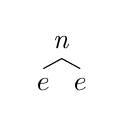
\begin{tikzpicture}[level distance=1.5em] \Tree [ .$\mathit{n}$ $e$ $e$ ]\end{tikzpicture}\end{array}
\end{alignat*}

Figure~\ref{chap4:syntax:syntax} presents the syntax of strategies in System S. We use $\mathbb{S}$ to denote the set of all strategies. Variables, atomic strategies, \sskip and \sabort are \textit{basic strategies}. Basic strategies are not decomposable. An atomic strategy is simply a rewrite rule. For instance, the commutativity of addition $\mathit{add_{com}}$ and commutativity of multiplication $\mathit{mult_{com}}$ are atomic strategies:
\begin{align*}
    &\mathit{add_{com}}: a + b \rightsquigarrow b + a &\text{Commutativity of addition}\\
    &\mathit{mult_{com}}: a * b \rightsquigarrow b * a &\text{Commutativity of multiplication}
\end{align*}
$\sskip$ can always be executed successfully while executing $\sabort$ would always cause failure. To compose strategies, one can make use of \textit{combinators} including sequential composition ($\seqcomp$), left choice ($\lchoice$) and nondeterministic choice ($\choice$). Sequential composition instructs to execute two strategies one after the other. Left choice prefers executing the strategy at the left hand side of the combinator over the strategy at the right hand side of the operator while nondeterministic choice decides to execute one of the given two strategy nondeterministically. In addition, $\one$, $\some$ and $\all$ are \textit{traversals} that navigate within the AST. Intuitively, $\one(s)$ applies $s$ to one immediate sub-expression of an input expression, $\some(s)$ applies $s$ to as many immediate sub-expressions of an input expression as possible and   $\all(s)$ applies $s$ to all immediate sub-expressions of an input expression. Lastly, System S provides a \textit{fixed-point operator} to model recursion.
\begin{figure}
\begin{alignat*}{3}
    \text{Strategy}(\mathbb{S}) \quad
    s \ \metaDeff &\ \mathit{atomic}
    \cmid X \cmid \sskip \cmid \sabort
    \\ \cmid &s\seqcomp s
    \cmid s \lchoice s
    \cmid s \choice s
    \\ \cmid &\one(s)
    \cmid \some(s)
    \cmid \all(s)
    \\ \cmid &\mu X. s
\end{alignat*}
\caption{The Syntax of System S}
\label{chap4:syntax:syntax}
\end{figure}
\paragraph*{Comparison of the expressiveness to the original System S}One difference between our formalism and the original System S is that we abstract away the term building details for atomic strategies, instead modelling atomic strategies as partial functions. We believe that applying this abstraction does not limit the expressiveness of our system. In fact, the purpose of such design is to allow the flexibility of the term languages, not only limited to the original System S, but also capturing other strategic rewriting languages that use term constructs that are different from System S. Moreover, this design enables us to focus on reasoning about properties of compositions of rewriting strategies that hold independent of the term building behaviour.

\paragraph*{Composing strategies}We can compose strategies together with these combinators, traversals and the fixed-point operator to define more strategies. For example, we define a strategy $\try(s)$ using left choice and \sskip which attempts to apply a strategy $s$ to an input expression. If an error occurs, then it will leave the input expression unchanged by executing the strategy \sskip:
\[\try(s) \metaDef s \lchoice \sskip\]
With the fixed-point operator and sequential composition, we can then define a strategy $\mathit{repeat}(s)$ which keeps applying a strategy $s$ to an input expression until its no longer applicable:
\[\mathit{repeat}(s) \metaDef \mu X. \mathit{try}(s\seqcomp X)\]
With the fixed-point operator, the traversal $\mathit{one}(s)$ and left choice, we can define top-down and bottom-up traversals in an AST:
\begin{align*}
    &\mathit{topDown} (s) \metaDef \mu X. (s \lchoice \one(X))
    &\mathit{bottomUp} (s) \metaDef \mu X. (\one(X) \lchoice s)
\end{align*}
We can further compose $\mathit{repeat}(s)$ and $\mathit{topDown}(s)$ to define a strategy $\mathit{normalise}(s)$, which keeps applying a strategy $s$ to all sub-expressions of an input expression until it is no longer applicable:
\[\mathit{normalise} (s) \metaDef \mathit{repeat}(\mathit{topDown}(s))\]
The $\mathit{normalise}$ strategy is very commonly used for expressing program transformations. Given $\mathit{beta}$ and $\mathit{eta}$ reductions for $\lambda$-expressions, we can use the normalisation strategy $\mathit{normalise}(\mathit{beta} \lchoice \mathit{eta})$ for normalising an input $\lambda$-expression into its $\beta\eta$-normal form.

As previously mentioned, the composition of strategies can be invalid and the executions of strategies are not always successful. For instance, the strategy $\mathit{mult_{com}}\seqcomp\mathit{add_{com}}$ is not well composed since it cannot be successfully executed on any input expression. $\mathit{repeat}(\sskip)$ is a strategy that cannot terminate. Although $\mathit{normalise}(\mathit{beta} \lchoice \mathit{eta})$ can certainly be successfully executed on some input expressions, on other inputs it may not terminate. It is important to know that when it terminates, it will indeed leave the expression in $\beta\eta$-normal form.

To reason about the successful and unsuccessful executions of strategies, we design the \emph{location-based weakest precondition calculus} which is discussed in section~\ref{chap4:wp}. With this calculus, we are able to detect \emph{bad} strategies that do not have successful executions, like $\mathit{mult_{com}}\seqcomp\mathit{add_{com}}$ and $\mathit{repeat}(\sskip)$, by concluding that there is no input expression that can be successfully rewritten by such strategies into a desired form. Also, for a \emph{good} strategy that has successful executions, we are able to distinguish inputs that indeed lead to successful executions of the strategy and inputs that lead to erroneous or diverging executions. Such reasoning power is demonstrated in section~\ref{chap4:reasoning}.  

To design the location-based weakest precondition calculus, we need to understand the behaviours of executing these strategies in System S. Therefore, before introducing the calculus and its reasoning power, we firstly study the formal semantics of System S.

\section{The Semantics of System S}
\label{chap4:semantics}
For given collections of expressions $\mathbb{E}$, System S defines nondeterministic executions for given strategies that can result in expressions or errors. We extend the original System S by allowing divergence as a possible result of executing a strategy. Thus, applying a strategy to an expression can result in expressions, an error or divergence.

\subsection{The Plotkin Powerdomain}
\label{chap4:subsec:plotkin}
We provide a denotational semantics of System S as an instance of Plotkin's powerdomain construction
\citep{plotkin:powerdomain}, which allows us to assign least fixed points as the semantics of the
recursion construct. An \emph{$\omega$-complete partial order} (\emph{$\omega$-cpo}) is a partially
ordered set $(X,\preceq)$ in which each $\omega$-chain ($x_1 \preceq x_2 \preceq x_3 \preceq \dots$)
has a least upper bound. A function $f:X \rightarrow X$ on such a set is \emph{continuous} if for
each $\omega$-chain $x_1 \preceq x_2 \preceq x_3 \preceq \dots$ with least upper bound $x$, one has
that $f(x)$ is the least upper bound of the set $\{f(x_1),f(x_2),f(x_3),\dots\}$.
A continuous function is certainly \emph{monotone}, in the sense that $x_1 \preceq x_2$ implies
$f(x_1) \preceq f(x_2)$ -- this follows by considering the $\omega$-chain
$x_1 \preceq x_2 \preceq x_2 \preceq x_2 \preceq \dots$, and its least upper bound $x_2$.
Now Kleene's fixed-point theorem says that each continuous function $f$ on an $\omega$-cpo with a least
element has a least fixed point.

Consider a nondeterministic, possibly diverging, algorithm that transforms values into values.
If $\V$ is the set of values, this algorithm can be modelled as a function
$f:\V \rightarrow \Pow_{\neg \emptyset}(\V_\bot)$, where
$\Pow_{\neg \emptyset}(X)$ is the set of non-empty subsets of $X$, the non-empty-powerset, and
$\V_\bot:= \V \uplus \{\bot\}$ is the set in which we embed $\V$ together with a new element $\bot$. The newly added element $\bot$ represents
the outcome where the algorithm diverges.
We equip the set $\V_\bot$ with a partial order by defining:
\[x \preceq y \iff x = \bot \lor x = y\;.\]
This fits with the intuition that $\bot$ represents a computation that has not yet
terminated, and $x \preceq y$ holds when $y$ is a later stage of the computation $x$.\\

Terminated computations are identified by the values they compute. We compare
sets of values using the Egli-Milner ordering:\vspace{1ex}\\
\( A \preceq B 
\iff (\forall x \in A.\; \exists y \in B.\; x \preceq y) \land (\forall y \in
B.\; \exists x \in A.\; x \preceq y)\)\vspace{1ex}

\begin{wrapfigure}{r}{0.37\textwidth}
  \vspace{-40pt}
  \begin{center}
    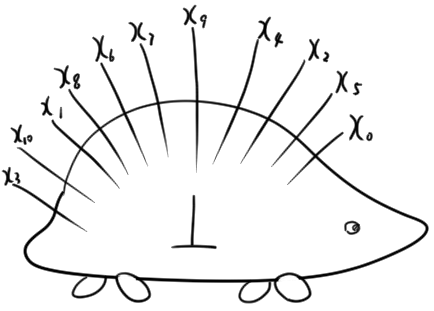
\includegraphics[width=0.3\textwidth]{porcupine.png}
  \end{center}
\end{wrapfigure}%

\noindent Lifting a partial order from elements to sets in this
fashion always yields a preorder. For a \emph{flat domain} $\V_\bot$, $\preceq$ is a partial order on
$\Pow_{\neg \emptyset}(\V_\bot)$. It is characterised by:
\begin{align*}
     &A \preceq B \iff  A = B \lor ((\bot \in A) \land A {\setminus} \{\bot\} \subseteq B)  &\qquad\qquad\text{\centering(Porcupine ordering)}
\end{align*}
The resulting poset $\Pow_{\neg \emptyset}(\V_\bot)$ is an $\omega$-cpo.
Each $\omega$-chain either enters a spine of the
porcupine, and thus contains a largest element which is its least upper bound,
or $\bot$ is a member of all elements in the chain, so that its least upper bound is simply the union of all sets in the chain.

\paragraph*{Aside on the powerdomain construction and the Egli-Milner ordering.}
To give some further insight into the powerdomain construction and the Egli-Milner ordering, recall the following well-known characterisation. \citet[Remark after Lemma~3.5]{hennessy-plotkin:plotkin-powerdomain} show that
\citepos{plotkin:powerdomain} powerdomain construction extends to all
$\omega$-complete partial orders (\wcpo{}s) by sending each \wcpo{} to
the \emph{free} semi-lattice over it. In detail, given an \wcpo{} $X$,
we define a \emph{free semi-lattice over $X$} as an \wcpo{} $DX$,
together with a Scott-continuous function $\eta : X \to DX$ and a
Scott-continuous binary operation: $\vee : (DX)^2 \to DX$ that is
associative, commutative, and idempotent. A free semi-lattice always
exists, but its explicit description may be complicated.
\citeauthor{hennessy-plotkin:plotkin-powerdomain} show that, when
\wcpo{} is $\omega$-algebraic, we can construct the free semi-lattice
explicitly by taking $DX := \Pow_{\lnot \emptyset}X$ to be the
powerdomain construction with the Egli-Milner ordering, $\eta(x) :=
\{x\}$ as the embedding of $X$ into this semi-lattice, and sub-set
union as the binary operation.  So in a specific and technical sense,
the powerdomain $DX$ is the simplest extension of the \wcpo{} $X$ with
an associative, idempotent and commutative binary operator.
\begin{flushright}
\vspace*{-1em}
	\textit{(end of aside)}
\end{flushright}

In our mechanised Isabelle/HOL formalisation, we opt to use posets
that are complete with respect to all chains, not merely countable or directed
ones, without maintaining continuity as an assumption. The stronger
assumption on posets allows us to weaken the assumption on functions:
we only require monotonicity to ensure existence of fixed points. This
choice was made purely for ease of formalisation, as Isabelle/HOL
already includes a library for chain-complete partial orders. While this means that our domain may contain monotone functions that do not correspond to any expressible strategy, and that \citeauthor{hennessy-plotkin:plotkin-powerdomain}'s characterisation does not directly apply, our meta-theoretic results below
show how to relate our semantics to the operational semantics, and our
reasoning examples show that this semantics suffices to reason about
practically interesting examples. We conjecture that our results will easily carry over to a semantics defined with \wcpo{}s.
% and we are currently developing an Isabelle/HOL library for \wcpo{}s that will allow us to confirm this conjecture.

\subsection{Formalised Denotational Semantics}
\label{chap4:denotational}
We now present and discuss the denotational semantics for
System S, capturing successful and erroneous executions of strategies
as well as nondeterminism, divergence and recursion.  A strategy is a
nondeterministic algorithm/function that rewrites expressions into expressions.
This nondeterministic algorithm can sometimes yield an error $\err$
instead of an expression, and it might fail to terminate.  In the
latter case, we say that it yields the value $\dive$.  Formally, we instantiate
Plotkin's powerdomain construction from
the previous section by setting $\V := \mathbb{E} \cup \{\err\}$ and
$\bot := \dive$, noting it is a flat domain.
We denote the resulting powerdomain by:
\begin{gather*}\mathfrak{D}_p \metaDef \Pow_{\neg \emptyset}(\mathbb{E} \cup \{\err\} \cup \{\dive\}) \quad \text{ordered by:}\\
A \preceq B \iff  A = B \lor ((\dive \in A) \land A {\setminus} \{\dive\} \subseteq B)
\end{gather*}

We define the denotational semantics of System S over the point-wise lifting of
the powerdomain:
\begin{align*}
    \mathfrak{D} = \mathbb{E} \to \mathfrak{D}_p
\end{align*}
To define the denotational semantics of strategies in a concise
manner, we provide semantic combinators and traversals that
encapsulate the meaning of syntactic combinators and traversals.

Figure~\ref{chap4:semantics:combinators} illustrates the definitions of the combinators. The definition of sequential composition $s{\sseqcomp} t$ is straightforward, indicating that the execution of the strategy $t$ depends on the result of applying $s$ to the input expression $e$. If applying $s$ to $e$ results in an error or divergence, the sequential composition will produce an error and divergence, respectively. Otherwise, the result of the sequential composition $s {\sseqcomp} t$ is produced by applying $t$ to the expression obtained by the execution of $s$.
The definition of left choice $s{\slchoice} t$ prioritises the execution of the strategy $s$ over~$t$. The strategy $t$ will only be executed if the execution of $s$ produces an error.
Our treatment of nondeterminism is \emph{demonic} with respect to divergence while \emph{angelic} with respect to errors. If either the execution of $s$ or $t$ divergences, then the nondeterministic choice $s {\schoice} t$ diverges as well. The nondeterministic choice will only result in an error if both executions of $s$ and $t$ result in an error. When both $s$ and $t$ give cause for a successful execution, the choice is nondeterministic.
\begin{figure}
\begin{align*}
    &(\sseqcomp) : \mathfrak{D} \rightarrow \mathfrak{D} \rightarrow \mathfrak{D}\\
    &(s \sseqcomp t) (e) = \bigcup \{t(e') \barr e' \in s(e) \cap \mathbb{E} \} \cup \{r \barr r\in s(e) \cap \{\dive, \err\}\}
    \intertext{\centering(Sequential composition)}
    &(\slchoice) : \mathfrak{D} \rightarrow \mathfrak{D} \rightarrow \mathfrak{D}\\
    &(s \slchoice t) (e) = (s(e) \setminus \{\err\}) \cup \{e' \barr e' \in t(e) \land \err \in s(e) \} \intertext{\centering(Left choice)}
    &(\schoice) : \mathfrak{D} \rightarrow \mathfrak{D} \rightarrow \mathfrak{D} \\
    &\begin{array}{@{}l@{\;}c@{\;}l}(s \schoice t)(e)  &=& \{e' \barr e' \in s(e) \cap \mathbb{E}\}
    \cup \{\dive \barr \dive \in s(e)\}\\
    &\cup& \{e' \barr e' \in t(e) \cap \mathbb{E}\}
    \cup \{\dive \barr \dive \in t(e)\}
    \cup \{\err \barr \err \in s(e) \cap t(e)\}
    \end{array}
    \intertext{\centering(Nondeterministic choice)}
\end{align*}
\vspace{-3em}
\caption{Semantic Combinators of System S}
\label{chap4:semantics:combinators}
\end{figure}

These combinators are sufficient for composing strategies applied to the root of an AST.
System S also provide traversals $\one$, $\some$ and $\all$ to apply strategies to sub-expressions. Their semantics are shown in figure~\ref{chap4:semantics:traversals}.
\begin{figure}
\begin{align*}
    &(\mathit{one_s}) : \mathfrak{D} \rightarrow \mathfrak{D}\\
    &\begin{array}{@{}l@{\;}c@{\;}l}
    \mathit{one_s}(s)(e) &=&
    \{\begin{array}{@{}c@{}}\tikzset{level distance=18pt}\Tree [.$n$ $e_1'$ $e_2\phantom{'}$ ]\end{array} \barr e = \begin{array}{@{}c@{}} \Tree [.$n$ $e_1$ $e_2$ ]\end{array} \land e_1' \in s(e_1) \cap \mathbb{E} \}\\
    &\cup& \{\begin{array}{@{}c@{}} \tikzset{level distance=18pt} \Tree [.$n$ $e_1\phantom{'}$ $e_2'$ ]\end{array} \barr e = \begin{array}{@{}c@{}} \Tree [.$n$ $e_1$ $e_2$ ]\end{array} \land e_2' \in s(e_2) \cap \mathbb{E} \}\\
    &\cup& \{\dive \barr e = \begin{array}{@{}c@{}} \Tree [.$n$ $e_1$ $e_2$ ]\end{array} \land \dive \in s(e_1) \cup s(e_2) \}\\
    &\cup& \{\err \barr e = \mathit{Leaf} \lor (e = \begin{array}{@{}c@{}} \Tree [.$n$ $e_1$ $e_2$ ]\end{array} \land \err \in s(e_1) \cap s(e_2)) \}
    \end{array}
    \\[-1.0em]
    \intertext{\centering(One)}\\[-2.5em]
    &(\mathit{some_s}) : \mathfrak{D} \rightarrow \mathfrak{D}\\
    &\begin{array}{@{}l@{\;}c@{\;}l}
    \mathit{some_s}(s)(e) &=&
    \{\begin{array}{@{}c@{}}  \tikzset{level distance=18pt}
    \Tree [.$n$ $e_1'$ $e_2'$ ]\end{array} \barr e = \begin{array}{@{}c@{}} \Tree [.$n$ $e_1$ $e_2$ ]\end{array} \land e_1' \in s(e_1) \cap \mathbb{E} \land e_2' \in s(e_2) \cap \mathbb{E} \} \\
    &\cup& \{\begin{array}{@{}c@{}} \tikzset{level distance=18pt}\Tree [.$n$ $e_1'$ $e_2\phantom{'}$ ]\end{array} \barr e = \begin{array}{@{}c@{}} \Tree [.$n$ $e_1$ $e_2$ ]\end{array} \land e_1' \in s(e_1) \cap \mathbb{E}\land \err \in s(e_2)\} \\
    &\cup& \{\begin{array}{@{}c@{}}  \tikzset{level distance=18pt}\Tree [.$n$ $e_1\phantom{'}$ $e_2'$ ]\end{array} \barr e = \begin{array}{@{}c@{}} \Tree [.$n$ $e_1$ $e_2$ ]\end{array} \land e_2 \in s(e_2) \cap \mathbb{E} \land \err \in s(e_1) \}\\
    &\cup& \{\dive \barr e = \begin{array}{@{}c@{}} \Tree [.$n$ $e_1$ $e_2$ ]\end{array} \land \dive \in s(e_1) \cup s(e_2) \}\\
    &\cup& \{\err \barr e = \mathit{Leaf} \lor (e = \begin{array}{@{}c@{}} \Tree [.$n$ $e_1$ $e_2$ ]\end{array} \land \err \in s(e_1) \cap s(e_2)) \}
    \end{array}\\[-1.0em]
    \intertext{\centering(Some)}\\[-2.5em]
    &(\mathit{all_s}) : \mathfrak{D} \rightarrow \mathfrak{D}\\
    &\begin{array}{@{}l@{\;}c@{\;}l}
    \mathit{all_s}(s)(e) &=&
    \{\mathit{Leaf} \barr e = \mathit{Leaf} \}\\
    &\cup& \{\begin{array}{@{}c@{}} \tikzset{level distance=18pt}\Tree [.$n$ $e_1'$ $e_2'$ ]\end{array} \barr e = \begin{array}{@{}c@{}} \Tree [.$n$ $e_1$ $e_2$ ]\end{array} \land e_1' \in s(e_1) \cap \mathbb{E} \land e_2' \in s(e_2) \cap \mathbb{E} \} \\
    &\cup& \{\dive \barr e = \begin{array}{@{}c@{}} \Tree [.$n$ $e_1$ $e_2$ ]\end{array} \land \dive \in s(e_1) \cup s(e_2) \}\\
    &\cup& \{\err \barr e = \begin{array}{@{}c@{}} \Tree [.$n$ $e_1$ $e_2$ ]\end{array} \land \err \in s(e_1) \cup s(e_2)\}
    \end{array}\\[-1.0em]
    \intertext{\centering(All)}
\end{align*}
\vspace{-4.0em}
\caption{Semantic Traversals of System S}
\label{chap4:semantics:traversals}
\end{figure}
The traversal $\ones(s)(e)$ nondeterministically chooses one immediate sub-expression of $e$ and applies strategy $s$ to it. The treatment of nondeterminism here is again demonic with respect to divergence and angelic with respect to errors.
If applying $s$ to one of the sub-expressions results in divergence, $\ones(s)$ will diverge. An error will only occur when $e$ has no sub-expression or applying $s$ to all sub-expressions of $e$ results in error.
The traversal $\somes(s)(e)$ applies $s$ to as many immediate sub-expressions of $e$ as possible. Its divergence and erroneous situations are the same as $\ones$.
The successful execution of $\alls(s)$ on an input expression~$e$ requires successful application of $s$ to all immediate sub-expressions of $e$ or $e$ being a $\mathit{Leaf}$. If applying $s$ to one sub-expression leads to an error or divergence, $\alls(s)(e)$ yields $\err$ or $\dive$, respectively.
For simplicity of the presentation and illustration, we have restricted ourselves to binary trees in this paper. However, the traversals can easily be generalised to ASTs with wider branching.

With the semantic combinators and semantic traversals introduced, we provide the denotational semantics for System S shown in figure~\ref{chap4:semantics:denotational}. The semantics of a strategy is modelled as a function that takes in a \emph{semantic environment} $\xi$, which is a function mapping variables to elements of $\mathfrak{D}$.

\begin{figure}[t]
\begin{align*}
    \text{Variable}(\mathbb{V}) \quad &X\; Y\; Z \dots \\
    \text{Semantic Environment}(\Gamma_S) \quad &\xi : \mathbb{V} \to \mathfrak{D}
\end{align*}
\vspace{-3.0em}
\begin{align*}
    &\llbracket \,\mathbb{S}\, \rrbracket : \Gamma_S \rightarrow \mathfrak{D}\\
    &\llbracket X \rrbracket \xi = \xi X \\
    &\llbracket \atomic \rrbracket \xi = \lambda e. \{\atomic(e) \barr \atomic(e)\, \tdef \} \cup \{\err \barr \atomic(e)\, \tundef\}\;\,\\
    &\llbracket \sskip \rrbracket \xi = \lambda e. \{e\} \\
    &\llbracket \sabort \rrbracket \xi = \lambda e. \{\err\}
\end{align*}
\vspace{-3.0em}
\begin{align*}
    &\llbracket s \seqcomp t \rrbracket \xi = \llbracket s \rrbracket \xi \sseqcomp \llbracket t \rrbracket \xi &\text{(Sequential composition)}\\
    &\llbracket s \lchoice t \rrbracket \xi = \llbracket s \rrbracket \xi \slchoice \llbracket t \rrbracket \xi &\text{(Left choice)}\\
    &\llbracket s \choice t \rrbracket \xi = \llbracket s \rrbracket \xi \schoice \llbracket t \rrbracket \xi &\text{(Nondeterministic choice)}\\
    &\llbracket \one(s) \rrbracket \xi = \ones (\llbracket s \rrbracket \xi) &\text{(One)}\\
    &\llbracket \some(s) \rrbracket \xi = \somes (\llbracket s \rrbracket \xi) &\text{(Some)}\\
    &\llbracket \all(s) \rrbracket \xi = \alls (\llbracket s \rrbracket \xi) &\text{(All)} \\
    &\llbracket \mu X. s\rrbracket \xi = \mu \mathcal{X}. \llbracket s \rrbracket (\xi[X \mapsto \mathcal{X}]) &\text{(Fixed point)}
\end{align*}
\vspace{-1.5em}
\caption{Denotational Semantics of System S}
\label{chap4:semantics:denotational}
\end{figure}

The semantics of a variable consists of looking up the variable in a given semantic environment. We model an atomic strategy as a partial function, which can successfully rewrite an input expression into an output expression when it is defined for the input expression. When an atomic strategy is not defined for an input expression, applying it to the input expression will result in an error. \sskip~is a strategy that always rewrites an input expression to itself while \sabort~is a strategy that always produces an $\err$. The denotational semantics of combinators and traversals are straightforwardly defined with the
semantic combinators and traversals. Lastly, the semantics of the fixed-point operator is the least fixed point in our domain, where we extend the semantic environment with a mapping from the syntactic fixed-point variable to the fixed point in our domain. We denote this environment extension with the syntax $\xi[X \mapsto d]$.

\paragraph*{The denotational semantics is monotone} Given two environments $\xi_1$ and $\xi_2$, if the values obtained from looking up the variables in the environments satisfy the ordering $\xi_1(X) \preceq \xi_2(X)$ for any variable $X$, the values obtained from evaluation of a strategy $s$ with these environments should also satisfy the ordering $\llbracket s \rrbracket\xi_1 \preceq \llbracket s \rrbracket\xi_2$. Formally, we present the monotonicity theorem~\ref{chap4:semantics:monotonicity}:
\begin{theorem}[Semantics monotonicity theorem]
For given environments $\xi_1$ and $\xi_2$, and strategy $s$ we have:
\vspace{-1.0em}
\begin{align*}
    \inferrule{\forall X. \xi_1(X) \preceq \xi_2(X)}{\llbracket s \rrbracket\xi_1 \preceq \llbracket s \rrbracket\xi_2}
\end{align*}
\label{chap4:semantics:monotonicity}
\end{theorem}
\vspace{-1.0em}
We prove this theorem in Isabelle/HOL by structural induction on the strategy $s$.

\subsection{Formalised Big-Step Operational Semantics}
\label{chap4:operational}
In this section, we present the formalised big-step operational semantics of System S, with our extension allowing for divergent strategies. Figure~\ref{chap4:semantics:operational-p1} depicts the big-step operational semantics for the non-diverging cases of System S. These cases are essentially the same as those of \citet{VISSER1998422}, albeit with the aforementioned simplification to binary trees applied.\footnote{\citet{VISSER1998422} denote error by $\uparrow$.} The semantic rules are given in a straightforward way.
\begin{figure}[t]
\vspace{1em}
\begin{mathparpagebreakable}
%%% Line 1
    \inferrule*[right={\scriptsize (Skip)}] { }
    {e \xrightarrow[]{\text{\tiny SKIP}} e}

    \inferrule*[right={\scriptsize (Abort)}] { }
    {e \xrightarrow[]{\text{\tiny ABORT}} \err}

    \inferrule*[right={\scriptsize (Atomic)}] { }
    {e \xrightarrow[]{\text{\tiny \atomic}} \mathit{atomic} (e)} \\

%%% Line 2
    \inferrule*[right={\scriptsize (SeqComp)}]{e \xrightarrow[]{s_1} e_1 \\ e_1 \xrightarrow[]{s_2} e_2}
    {e \xrightarrow[]{s_1 \seqcomp s_2} e_2}

	\hspace{-2mm}
    \inferrule*[right={\scriptsize (SeqCompErr(1))}]{e \xrightarrow[]{s_1} \err}
    {e \xrightarrow[]{s_1 \seqcomp s_2} \err}
    \hspace{-2mm}

    \inferrule*[right={\scriptsize (SeqCompErr(2))}]{e \xrightarrow[]{s_1} e_1 \\ e_1 \xrightarrow[]{s_2} \err}
    {e \xrightarrow[]{s_1 \seqcomp s_2} \err}

%%% Line 3
    \inferrule*[right={\scriptsize (LChoice (L))}]{e \xrightarrow[]{s_1} e_1}
    {e \xrightarrow[]{s_1 \lchoice s_2} e_1}

    \inferrule*[right={\scriptsize (LChoice (R))}]{e \xrightarrow[]{s_1} \err \\ e \xrightarrow[]{s_2} e_2}
    {e \xrightarrow[]{s_1 \lchoice s_2} e_2}

    \inferrule*[right={\scriptsize (LChoiceErr)}]{e \xrightarrow[]{s_1} \err \\ e \xrightarrow[]{s_2} \err}
    {e \xrightarrow[]{s_1 \lchoice s_2} \err}

%%% Line 4
    \inferrule*[right={\scriptsize (Choice(L))}]{e \xrightarrow[]{s_1} e_1}
    {e \xrightarrow[]{s_1 \choice s_2} e_1}

    \inferrule*[right={\scriptsize (Choice(R))}]{e \xrightarrow[]{s_2} e_2}
    {e \xrightarrow[]{s_1 \choice s_2} e_2}

    \inferrule*[right={\scriptsize (ChoiceErr)}]{e \xrightarrow[]{s_1} \err \\ e \xrightarrow[]{s_2} \err}
    {e \xrightarrow[]{s_1 \choice s_2} \err}\\

%%% Line 5
    \inferrule*[right={\scriptsize (FixedPoint)}]{e \xrightarrow[]{s[X := \mu X .s]} e_1}
    {e \xrightarrow[]{\mu X .s} e_1}
\qquad\qquad\qquad
    \inferrule*[right={\scriptsize (FixedPointErr)}]{e \xrightarrow[]{s[X := \mu X .s]} \err}
    {e \xrightarrow[]{\mu X .s} \err}
\end{mathparpagebreakable}
\caption{Big-step operational semantics of non-diverging cases for basic strategies, combinators, and the fixed-point operator}
\label{chap4:semantics:operational-p1}
\vspace{-1em}
\end{figure}

\begin{figure}
\begin{mathparpagebreakable}
\inferrule*[right={\scriptsize (One(Id))}]{ }
    {\mathit{Leaf} \xrightarrow[]{\mathit{one} (s)} \err}

    \inferrule*[right={\scriptsize (Some(Id))}]{ }
    {\mathit{Leaf} \xrightarrow[]{\mathit{some} (s)} \err}

    {\inferrule*[right={\scriptsize (All(Id))}]{ }
    {\mathit{Leaf}\xrightarrow[]{\mathit{all} (s)} \mathit{Leaf}}}
\\

%%% Line 7
    \inferrule*[right={\scriptsize (One(L))}]{e_1 \xrightarrow[]{s} e_1'}
    {\begin{array}{@{}c@{}} \Tree [.$n$ $e_1$ $e_2$ ]\end{array} \xrightarrow[]{\mathit{one} (s)} \begin{array}{@{}c@{}} \tikzset{level distance=18pt}\Tree [.$n$ $e_1'$ $e_2\phantom{'}$ ]\end{array}}

    \hspace{-5mm}
    \inferrule*[right={\scriptsize (One(R))}]{e_2 \xrightarrow[]{s} e_2'}
    {\begin{array}{@{}c@{}} \Tree [.$n$ $e_1$ $e_2$ ]\end{array} \xrightarrow[]{\mathit{one} (s)} \begin{array}{@{}c@{}} \tikzset{level distance=18pt}\Tree [.$n$ $e_1\phantom{'}$ $e_2'$ ]\	\end{array}}
    \hspace{-5mm}

    \inferrule*[right={\scriptsize (OneErr)}]{e_1 \xrightarrow[]{s} \err \\ e_2 \xrightarrow[]{s} \err}
    {\begin{array}{@{}c@{}} \Tree [.$n$ $e_1$ $e_2$ ]\end{array} \xrightarrow[]{\mathit{one} (s)} \err}\\

 %%%% Line 8a
    \inferrule*[right={\scriptsize (Some(L))}]{e_1 \xrightarrow[]{s} e_1' \\ e_2 \xrightarrow[]{s} \err}
    {\begin{array}{@{}c@{}} \Tree [.$n$ $e_1$ $e_2$ ]\end{array} \xrightarrow[]{\mathit{some} (s)} \begin{array}{@{}c@{}} \tikzset{level distance=18pt}\Tree [.$n$ $e_1'$ $e_2\phantom{'}$ ]\end{array}}

    \inferrule*[right={\scriptsize (Some(R))}]{e_1 \xrightarrow[]{s} \err \\ e_2 \xrightarrow[]{s} e_2'}
    {\begin{array}{@{}c@{}} \Tree [.$n$ $e_1$ $e_2$ ]\end{array} \xrightarrow[]{\mathit{some} (s)} \begin{array}{@{}c@{}} \tikzset{level distance=18pt}\Tree [.$n$ $e_1\phantom'$ $e_2'$ ]\end{array}}\\

 %%%% Line 8b
    \inferrule*[right={\scriptsize (Some)}]{e_1 \xrightarrow[]{s} e_1' \\ e_2 \xrightarrow[]{s} e_2'}
    {\begin{array}{@{}c@{}} \Tree [.$n$ $e_1$ $e_2$ ]\end{array} \xrightarrow[]{\mathit{some} (s)}\tikzset{level distance=18pt}\begin{array}{@{}c@{}} \Tree [.$n$ $e_1'$ $e_2'$ ]\end{array}}

    \inferrule*[right={\scriptsize (SomeErr)}]{e_1 \xrightarrow[]{s} \err \\ e_2 \xrightarrow[]{s} \err}
    {\begin{array}{@{}c@{}} \Tree [.$n$ $e_1$ $e_2$ ]\end{array} \xrightarrow[]{\mathit{some} (s)} \err}

 %%%% Line 9
    \inferrule*[right={\scriptsize (All)}]{e_1 \xrightarrow[]{s} e_1' \\ e_2 \xrightarrow[]{s} e_2'}
    {\begin{array}{@{}c@{}} \Tree [.$n$ $e_1$ $e_2$ ]\end{array} \xrightarrow[]{\mathit{all} (s)} \begin{array}{@{}c@{}} \tikzset{level distance=18pt}\Tree [.$n$ $e_1'$ $e_2'$ ]\end{array}}

    \inferrule*[right={\scriptsize (AllErr(L))}]{e_1 \xrightarrow[]{s} \err}
    {\begin{array}{@{}c@{}} \Tree [.$n$ $e_1$ $e_2$ ]\end{array} \xrightarrow[]{\mathit{all} (s)} \err}

    \inferrule*[right={\scriptsize (AllErr(R))}]{e_2 \xrightarrow[]{s} \err}
    {\begin{array}{@{}c@{}} \Tree [.$n$ $e_1$ $e_2$ ]\end{array} \xrightarrow[]{\mathit{all} (s)} \err}
\end{mathparpagebreakable}
\caption{Big-step operational semantics of non-diverging cases for traversals}
\label{chap4:semantics:operational-p2}
\vspace{-1em}
\end{figure}

On top of these rules for terminating cases, we define the semantics for divergence as the \emph{coinductive} judgement \cite{LEROY2009284} satisfying the rules shown in figure \ref{chap4:semantics:operational-div}. Here we use \plat{$e \xrightarrow[\infty]{s}$} to indicate that the evaluation of an expression $e$ by a strategy $s$ leads to divergence.
\begin{figure}
\begin{mathpar}
\begin{array}{ccc}
 %%%% Line 1
    \inferrule*[right={\scriptsize (SeqCompDiv(1))}]{e \xrightarrow[\infty]{s_1}}
    {e \xrightarrow[\infty]{s_1 \seqcomp s_2}}
&\quad &
    \inferrule*[right={\scriptsize (SeqCompDiv(2))}]{e \xrightarrow[]{s_1} e_1 \\ e_1 \xrightarrow[\infty]{s_2}}
    {e \xrightarrow[\infty]{s_1 \seqcomp s_2}}\\[1em]
 %%%% Line 2
    \inferrule*[right={\scriptsize (LChoiceDiv(1))}]{e \xrightarrow[\infty]{s_1}}
    {e \xrightarrow[\infty]{s_1 \lchoice s_2}}
&&
    \inferrule*[right={\scriptsize (LChoiceDiv(2))}]{e \xrightarrow[]{s_1} \err \\ e \xrightarrow[\infty]{s_2}}
    {e \xrightarrow[\infty]{s_1 \lchoice s_2}}\\[1em]
 %%%% Line 3
    \inferrule*[right={\scriptsize (ChoiceDiv(1))}]{e \xrightarrow[\infty]{s_1}}
    {e \xrightarrow[\infty]{s_1 \choice s_2}}
&&
    \inferrule*[right={\scriptsize (ChoiceDiv(2))}]{e \xrightarrow[\infty]{s_2}}
    {e \xrightarrow[\infty]{s_1 \choice s_2}}\\[1em]
 %%%% Line 4
    \inferrule*[right={\scriptsize (OneDiv(1))}]{e_1 \xrightarrow[\infty]{s}}
    {\begin{array}{@{}c@{}} \Tree [.$n$ $e_1$ $e_2$ ]\end{array} \xrightarrow[\infty]{\mathit{one} (s)}}
&&
    \inferrule*[right={\scriptsize (OneDiv(2))}]{e_2 \xrightarrow[\infty]{s}}
    {\begin{array}{@{}c@{}} \Tree [.$n$ $e_1$ $e_2$ ]\end{array} \xrightarrow[\infty]{\mathit{one} (s)}}\\[1em]
 %%%% Line 5
    \inferrule*[right={\scriptsize(SomeDiv (1))}]{e_1 \xrightarrow[\infty]{s}}
    {\begin{array}{@{}c@{}} \Tree [.$n$ $e_1$ $e_2$ ]\end{array} \xrightarrow[\infty]{\mathit{some} (s)}}
&&
    \inferrule*[right={\scriptsize(SomeDiv (2))}]{e_2 \xrightarrow[\infty]{s}}
    {\begin{array}{@{}c@{}} \Tree [.$n$ $e_1$ $e_2$ ]\end{array} \xrightarrow[\infty]{\mathit{some} (s)}}\\[1em]
 %%%% Line 6
    \inferrule*[right={\scriptsize(AllDiv (1))}]{e_1 \xrightarrow[\infty]{s}}
    {\begin{array}{@{}c@{}} \Tree [.$n$ $e_1$ $e_2$ ]\end{array} \xrightarrow[\infty]{\mathit{all} (s)}}
&&
    \inferrule*[right={\scriptsize(AllDiv (2))}]{e_2 \xrightarrow[\infty]{s}}
    {\begin{array}{@{}c@{}} \Tree [.$n$ $e_1$ $e_2$ ]\end{array} \xrightarrow[\infty]{\mathit{all} (s)}}\\
\end{array}\\

 %%%% Line 7
    \inferrule*[right={\scriptsize (FixedPointDiv)}]{e \xrightarrow[\infty]{s[X := \mu X .s]}}
    {e \xrightarrow[\infty]{\mu X .s}}
\end{mathpar}
\caption{Big-step operational semantics of diverging cases}
\label{chap4:semantics:operational-div}
\end{figure}

\subsection{The Denotational Semantics is Equivalent to The Big-Step Operational Semantics}
\label{chap4:equaivalence}
In section~\ref{chap4:denotational} and section~\ref{chap4:operational}, we have provided two styles of semantics for System S. It is essential to prove that these two semantics are equivalent, since we would like our formal semantics to provide unambiguous and unique interpretation of strategies in System S. In addition, with the equivalence of these two semantics established, we only need to refer to one of them to prove some properties of System S and they should also hold for the other semantics.

We reason about the equivalence between the denotational semantics and big-step operational semantics via computational soundness and computational adequacy theorems. More specifically, we have a pair of computational soundness and adequacy theorems to relate the non-diverging cases and a pair of computational soundness and adequacy theorems to relate the diverging cases.

Firstly, we show that if an expression $e$ is evaluated to another expression or an error using the big-step operational semantics of a strategy $s_\clubsuit$, this result must also be in the set obtained by executing the denotational semantics of $s_{\clubsuit}$ with the given expression $e$. Formally, this is described by our first computational soundness theorem \ref{chap4:semantics:soundness-one}. The subscript $\clubsuit$ indicates that $s_{\clubsuit}$ is a \emph{closed} strategy: a strategy with no free variables, i.e. $\mathit{fv}(s_\clubsuit) = \emptyset$.

\begin{theorem}[Computational soundness theorem one]
For a given closed strategy $s_\clubsuit$, and any environment $\xi$, we have for an arbitrary expression $e$ and result $r$:
\begin{mathpar}
    \inferrule*{e \xrightarrow[]{s_\clubsuit} r}{r \in \llbracket s_\clubsuit \rrbracket \xi e}
\end{mathpar}
\label{chap4:semantics:soundness-one}
\vspace{-1.5em}
\end{theorem}
We prove this theorem by induction on the derivation of $e \xrightarrow[]{s_\clubsuit} r$ from the rules of figure~\ref{chap4:semantics:operational-p1}. As the strategy $s_\clubsuit$ is always closed, to instantiate our inductive hypothesis in the cases for the fixed-point operator, we make use of the following substitution lemma~\ref{chap4:semantics:substitution-one} to semantically relate the syntactic substitution of a closed strategy $s_\clubsuit$ for a variable $X$ in $s$ with the strategy $s$ under the environment where $X$ maps to the semantics of $s_\clubsuit$.
\begin{lemma}[Substitution lemma one]
\begin{align*}
\llbracket s[X := s_\clubsuit] \rrbracket \xi = \llbracket s \rrbracket \xi [X \mapsto (\llbracket s_\clubsuit \rrbracket\xi)]
\end{align*}
\label{chap4:semantics:substitution-one}
\vspace{-1.5em}
\end{lemma}
\noindent
This lemma can easily be generalised to allow $s_\clubsuit$ to instead be an open strategy, so long as $X$ is not free in $s_\clubsuit$, however our operational semantics only ever substitutes closed strategies, thus this generalisation is not necessary for proving our semantic equivalence theorems.

We now prove a computational adequacy theorem, the  converse of the computational soundness theorem \ref{chap4:semantics:soundness-one}. It states that if a non-diverging result $r$ is one of the results of the denotational semantics for a closed strategy $s_\clubsuit$ with an input expression $e$, then the big-step operational semantics of $s_\clubsuit$ with the input expression $e$ will produce the same result.
\begin{theorem}[Computational adequacy theorem one] For an expression $e$, result $r$, and closed strategy~$s_\clubsuit$ we have:
\begin{mathpar}
   \inferrule{r \in \llbracket s_\clubsuit \rrbracket \xi e \\ r \neq \dive }{e \xrightarrow[]{s_\clubsuit} r}
\end{mathpar}
\label{chap4:semantics:adequacy-one}
\vspace{-1.5em}
\end{theorem}
\noindent
To prove this theorem, we  first generalise to open strategies. To do this, we define an
approximation relation between a closed strategy and an element of our domain, and state an
approximation lemma. Here, we employ, for a simultaneous substitution $\theta: \mathbb{V} \to
\mathbb{S}_{\clubsuit}$, the notation $s[\theta]$ for the application of $\theta$ to all free variables in $s$.

\begin{definition}[Approximation relation one] Given a closed strategy $s_\clubsuit$ and a function $d \in\mathfrak{D}$, we say $s_\clubsuit \approximation d$ if and only if for any given input expression $e$, when $r$ is a non-diverging result obtained by applying $d$ to $e$, $r$ will also be the result of evaluating the big-step operational semantics of $s_\clubsuit$ with the input expression $e$.
\begin{align*}
    s_\clubsuit \approximation d  \iff \forall e\; r.\; r \in d(e)\cap(\mathbb{E}\cup\{\err\}) \Rightarrow e \xrightarrow[]{s_\clubsuit} r
\end{align*}
\end{definition}
\begin{lemma}[Approximation lemma one]
\begin{align*}
    \inferrule*[]{\forall y \in \mathit{fv}(s).\; \theta(y) \approximation \xi(y)\\ s_\clubsuit = s[\theta]}{s_\clubsuit \approximation \llbracket s \rrbracket \xi}
\end{align*}
\end{lemma}
The proof of this lemma is by induction on the strategy $s$, and Scott induction is required for the fixed point cases. From the approximation lemma, we prove the computational adequacy theorem \ref{chap4:semantics:adequacy-one} by setting $s := s_\clubsuit$. As there are no free variables in $s_\clubsuit$, the approximation relation trivially implies our goal.

The computational soundness and adequacy theorems presented above state that the denotational semantics and big-step operational semantics are equivalent for the non-diverging cases. Next, we present computational soundness and adequacy theorems for divergent strategies.

The computational soundness theorem for the diverging cases states that, if the evaluation of the big-step operational semantics of a closed strategy $s_\clubsuit$ with an input expression $e$ diverges, $\dive$ must be in the resulting set obtained by executing the denotational semantics of $s_\clubsuit$ with the given expression $e$.
\begin{theorem}[Computational soundness theorem two]
\begin{align*}
    \inferrule{e \xrightarrow[\infty]{s_\clubsuit}}{\dive \in \llbracket s_\clubsuit \rrbracket \xi e}
\end{align*}
\label{chap4:semantics:soundness-two}
\vspace{-1.3em}
\end{theorem}
Just as with computational adequacy for non-diverging cases, we must first generalise to open strategies. We define the second approximation relation together with an approximation lemma to prove this soundness theorem.
\begin{definition}[Approximation relation two] Given a closed strategy $s_\clubsuit$ and a function $d\in\mathfrak{D}$, we say $s_\clubsuit \approximationdiv d$ if and only if for any given input expression $e$, when evaluating the big-step operational semantics of $s_\clubsuit$ with the input expression $e$ diverges, $\dive$ will be obtained by applying $d$ to $e$, and we have the ordering $d(e) \preceq \llbracket s_\clubsuit \rrbracket \xi e$.
\begin{align*}
    s_\clubsuit \approximationdiv d \iff \forall e.\; (e \xrightarrow[\infty]{s_\clubsuit} \;\Rightarrow \dive \in d(e)) \land d(e) \preceq \llbracket s_\clubsuit \rrbracket \xi e
\end{align*}
\label{chap4:semantics:approximation-two}
\end{definition}
\begin{lemma}[Approximation lemma two]
\begin{align*}
    \inferrule*[]{\forall y \in \mathit{fv}(s).\; \theta(y) \approximationdiv \xi(y) \\ s_\clubsuit = s[\theta]}{s_\clubsuit \approximationdiv \llbracket s \rrbracket \xi}
\end{align*}
\label{chap4:semantics:approximation-lemma-two}
\vspace{-1.5em}
\end{lemma}
\noindent
The proof of this lemma is (again) by induction on the strategy $s$, where Scott induction is used for the fixed point cases. For the cases which involve terminating sub-steps, such as sequential composition or left choice, we make use of our soundness theorem for non-diverging cases, theorem~\ref{chap4:semantics:soundness-one}.
We utilise this approximation lemma \ref{chap4:semantics:approximation-lemma-two} to prove the computational soundness theorem~\ref{chap4:semantics:soundness-two}.

Lastly, we prove the computational adequacy theorem for the diverging cases, which is again the converse of the soundness theorem \ref{chap4:semantics:soundness-two}. It states that if $\dive$ is in a result of executing the denotational semantics of a closed strategy $s_\clubsuit$ with an input expression $e$, then evaluating the big-step operational semantics with the given expression $e$ leads to divergence.

\begin{theorem}[Computational adequacy theorem two]
    \begin{align*}
    \inferrule{\dive \in \llbracket s_\clubsuit \rrbracket \xi e}{e \xrightarrow[\infty]{s_\clubsuit}}
    \end{align*}
\label{chap4:semantics:adequacy-two}
\vspace{-1.5em}
\end{theorem}
We prove this by \emph{coinduction} over big-step operational semantics for diverging cases while making use of the computational adequacy theorem \ref{chap4:semantics:adequacy-one} for the non-diverging cases. Just as with our computational soundness proof for non-diverging cases, we work only with closed strategies $s_\clubsuit$, and rely on our substitution lemma~\ref{chap4:semantics:substitution-one} for the fixed point cases.

With these two pairs of computational soundness and adequacy theorems, we can conclude that the denotational semantics and big-step operational semantics are equivalent. Formally, we obtain:
\begin{theorem}[Equivalence between semantics]
    \begin{align*}
    \llbracket s_\clubsuit\rrbracket \xi e =
    \{r \barr e \xrightarrow[]{s_\clubsuit} r \} \cup
     \{\dive \barr e \xrightarrow[\infty]{s_\clubsuit}\}
    \end{align*}
\label{chap4:semantics:equiv}
\vspace{-1.5em}
\end{theorem}
In this section, we have studied two styles of semantics of System S, namely a denotational semantics and a big-step operational semantics. To complete our semantic accounting, it may be worthwhile for us to study its small-step operational semantics in the future.

\section{Location-Based Weakest Precondition Calculus}
\label{chap4:wp}
As we have seen, a strategy either successfully rewrites an expression into another expression, generates an error, or fails to terminate.

Naturally, we care mainly about the \emph{successful} executions of a strategy. In particular, when it rewrites an input expression into another expression that satisfies a desired property. In order to formally understand successful and unsuccessful executions of strategies, we design and formalise a location-based weakest precondition calculus. Weakest preconditions were introduced by \citet{DBLP:journals/cacm/Dijkstra75}, as an axiomatic semantics for his guarded command language.
Different from other weakest precondition calculi, we introduce the notion of a \emph{location} in an AST as a parameter in our calculus for reasoning about traversals, which is discussed in section~\ref{chap4:wp:design}.
Before presenting the formal definition of the calculus, we recapitulate the definition of a weakest precondition.
\begin{definition}[Weakest precondition] Given a program $S$ and a postcondition $P$, the \textit{weakest precondition} $\mathit{wp}(S,P)$ is an assertion $R_w$ such that for any precondition $R$:
    \[\{R\} S \{P\} \Leftrightarrow (R \Rightarrow R_w)\]
\end{definition}
\noindent Here $\{R\} S \{P\}$ is a Hoare triple stating that $S$ will successfully terminate in a state satisfying assertion $P$ if the state before executing $S$ satisfies $R$. Intuitively, the weakest precondition of $S$ under $P$ characterises all those states that lead to successful termination in a state of $P$ when executing $S$.
In \citepos{DBLP:journals/cacm/Dijkstra75} calculus, a function $\mathit{wp}$ is defined which, given a program and an assertion as a postcondition, computes the weakest precondition inductively on the program structure. \citet{DBLP:conf/rex/BonsangueK92} extend Dijkstra's calculus to assign weakest preconditions for a fixed-point operator by additionally including a \emph{logic environment} as an input to the $\mathit{wp}$ function, which associates a predicate transformer with each variable. As we also have a fixed-point operator for general recursion, we do the same in this formalisation.

When dealing with strategies, assertions take the form of sets of expressions, and a state is an expression we are rewriting. Thus, the weakest precondition is a set of input expressions for a strategy to be applied to, such that the result of the application of the strategy will lead to another expression. That means the strategy will neither yield an error nor diverge. Moreover, the weakest precondition has to guarantee that an expression of the postcondition is reached.

\begin{definition}[Weakest must succeed precondition]
A \emph{weakest must succeed precondition} takes the form $wp_{\zeta \Vdash s@l}(P)$.
This is the set of those expressions that, by applying strategy \textit{s} at location \textit{l}
under the logic environment $\zeta$, will be successfully transformed into expressions satisfying $P$.
\label{chap4:wp:ms}
\end{definition}
To calculate this set of input expressions constituting the weakest must succeed precondition, we also introduce
the following auxiliary function. In fact, $wp_{\zeta \Vdash s@l}(P)$ and $wp_{\zeta \Vdash s@l}^\uparrow(P)$
will be defined by mutual induction.
\begin{definition}[Weakest may error precondition]
A \emph{weakest may error precondition} takes the form of $wp_{\zeta \Vdash s@l}^\uparrow(P)$.
This is the set of those expressions that, by applying strategy \textit{s} at location \textit{l}
under the logic environment $\zeta$, will be successfully transformed into expressions satisfying $P$, \textbf{or result in error}.
\label{chap4:wp:me}
\end{definition}

\subsection{Modelling Traversals}
\label{chap4:wp:design}
In definitions~\ref{chap4:wp:ms} and~\ref{chap4:wp:me}, we introduce the location for specifying the particular sub-expression to which the strategy $s$ should be applied. This allows us to express that after applying a strategy $s$ to the sub-expression \emph{at the location} $l$ of an input expression $e$, the input expression $e$ should be transformed into an expression that satisfies the postcondition $P$.
Consequently, the weakest precondition for traversals such as $\mathit{one}(s)$, $\mathit{some}(s)$, and $\mathit{all}(s)$ can be defined inductively in terms of the weakest precondition of $s$, just at different locations.

\citet{KIEBURTZ2001138} proposes an alternative approach, using modal logic for assertions about traversals. However, it is unclear how this technique could be used to define a complete calculus. We discuss this in section~\ref{related-work}.

A \emph{location} is essentially a path into the abstract syntax tree. Such a path consists of a sequence of positions, for our binary trees either left ($\mathscr{l}$) or right ($\mathscr{r}$). Positions are prepended to a location with $\triangleleft$ and appended with $\triangleright$. For instance, suppose we have an AST representing an arithmetic expression $1 + 3$, each sub-expression is located as:
\begin{align*}
    \begin{array}{@{}c@{}} 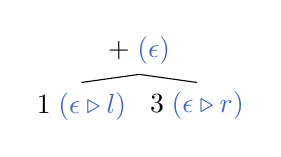
\begin{tikzpicture}[level distance=2em]\Tree [ .$+\;\text{\color{kirby-blue}($\epsilon$)}$ $1\;\text{\color{kirby-blue}($\epsilon\triangleright\mathscr{l}$)}$ $3\;\text{\color{kirby-blue}($\epsilon\triangleright\mathscr{r}$)}$ ] \end{tikzpicture}\end{array}
\end{align*}
With locations being introduced in the assertions, accompanied by the two helper functions $\mathit{lookup}$ and $\mathit{update}$ discussed in section~\ref{chap4:wp:calculus}, we can model the execution of a strategy at a given location in the input expression, which enables the assignments of weakest preconditions inductively for traversals just as with other operators.

\subsection{The Calculus}
\label{chap4:wp:calculus}
We now introduce the location-based weakest precondition calculus for System S in its full formal detail. We first provide definitions of helper functions and essential notations for the formalisation.
\begin{figure}[t]
\begin{align*}
    &\textit{lookup} : \mathbb{L} \to \mathbb{E} \rightharpoonup \mathbb{E} \quad (\text{We write it as }\pitchforkup_{l: \mathbb{L}}(e: \mathbb{E}) : (e' : \mathbb{E}))\\
    &\textit{lookup} \;\epsilon\; e = e\\[-.25em]
    &\textit{lookup} \;(\mathscr{l} \triangleleft l) \begin{array}{@{}c@{}} \Tree [.$n$ $e_1$ $e_2$ ]\end{array} = \textit{lookup} \;l\; e_1\\[-.25em]
    &\textit{lookup} \;(\mathscr{r} \triangleleft l)\; \begin{array}{@{}c@{}} \Tree [.$n$ $e_1$ $e_2$ ]\end{array} = \textit{lookup}\;l\; e_2\\
    &\textit{update} : \mathbb{L} \to \mathbb{E} \rightharpoonup \mathfrak{D}_p \to \mathfrak{D}_p \quad (\text{We write it as }(d: \mathfrak{D}_p)\boxRight_{l:\mathbb{L}} (e : \mathbb{E}) : (d' : \mathfrak{D}_p))\\
    &\textit{update} \;\epsilon\; e\; \mathit{xs} = \mathit{xs}\\[-.25em]
    &\textit{update} \;(\mathscr{l} \triangleleft l)\; \begin{array}{@{}c@{}} \Tree [.$n$ $e_1$ $e_2$ ]\end{array} \;\mathit{xs} = \{\begin{array}{@{}c@{}} 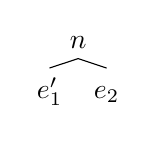
\begin{tikzpicture}[level distance=1.8em] \Tree [.$n$ $e_1'$ $\phantom{'}e_2\phantom{'}$ ]\end{tikzpicture}\end{array} \barr e_1' \in (\textit{update}\;l\;e_1\;\mathit{xs}) \cap \mathbb{E}\} \cup (\mathit{xs} \cap \{\err, \dive\})\\[-.25em]
    &\textit{update} \;(\mathscr{r} \triangleleft l)\; \begin{array}{@{}c@{}} \Tree [.$n$ $e_1$ $e_2$ ]\end{array}\; \mathit{xs} = \{\begin{array}{@{}c@{}} 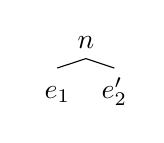
\begin{tikzpicture}[level distance=1.8em] \Tree [.$n$ $\phantom{'}e_1\phantom{'}$ $e_2'$ ]\end{tikzpicture}\end{array} \barr e_2' \in (\textit{update}\; l\; e_2\; \mathit{xs}) \cap \mathbb{E}\} \cup (\mathit{xs} \cap \{\err, \dive\})
\end{align*}
\caption{Helper functions}
\label{chap4:wp:lookup-update}
\end{figure}

To connect locations and expressions, we introduce two partial functions \textit{lookup} and \textit{update}, shown in figure~\ref{chap4:wp:lookup-update}. Given a location $l$
and an expression $e$, the partial function \textit{lookup} returns the sub-expression which is
located at the location $l$ in an expression $e$. The function is partial, as it is only defined
when the location $l$ actually exists in the expression $e$. The partial function \textit{update}
takes in a set $\mathit{xs} \in\mathfrak{D}_p$, and updates an expression $e$ at the
location $l$ with each expression in $\mathit{xs}$, resulting in a set of
expressions where each element is obtained by replacing the sub-expression of $e$ at the location
$l$ with an element of $\mathit{xs}$, with appropriate handling of errors and~divergence.

Figure~\ref{chap4:wp:notations} shows the essential notations for defining the weakest precondition calculus. Since we will again have fixed-point operators in the weakest precondition calculus, we need to ensure that least fixed points exist, by operating in a domain which is again a cpo, and show that our wp function is monotone with respect to that domain. The ordering of our domain $\mathfrak{D}_L$ is a point-wise lifted set ordering, of which the bottom element is the empty set.

Similar to the semantic environment introduced for the denotational semantics in figure~\ref{chap4:semantics:denotational}, the logic environment contains mappings of (fixed point) variables to an element of our logic domain (which is a function). Since we mutually define weakest must succeed preconditions and weakest may error preconditions, a fixed-point variable can map to two different functions. We use the tags $\cdot$ (must succeed) and $\uparrow$ (may error) to distinguish these two different mappings.

\begin{figure}[t]
\begin{align*}
\begin{aligned}[c]
\mathrm{Position} \quad &i \metaDef \quad \mathscr{l} \cmid \mathscr{r}\\
\mathrm{Variable}(\mathbb{V}) \quad &X\; Y\; Z \dots
\end{aligned}
\quad\quad\quad
\begin{aligned}[c]
\mathrm{Location}(\mathbb{L}) \quad &l \metaDef \quad \epsilon \cmid l \triangleright i \cmid i \triangleleft l\\
\mathrm{Tag}(\mathbb{T}) \quad &t \metaDef \quad \cdot \cmid \uparrow
\end{aligned}
\end{align*}
\begin{align*}
    \text{Logic Domain}\quad&\mathfrak{D}_L = \mathbb{L} \to \Pow(\mathbb{E}) \to \Pow(\mathbb{E})\\
    \text{Logic Environment}(\Gamma_L) \quad &\zeta : (\mathbb{V} \times \mathbb{T}) \to \mathfrak{D}_L
\end{align*}
\begin{align*}
&wp_{\zeta: \Gamma_L \Vdash s:\mathbb{S} @l:\mathbb{L}} (P : \Pow(\mathbb{E})) : (R_w : \Pow(\mathbb{E})) &\text{(Weakest must succeed precondition)}\\
&wp_{\zeta: \Gamma_L \Vdash s:\mathbb{S} @l:\mathbb{L}}^\uparrow (P : \Pow(\mathbb{E})) : (R_w : \Pow(\mathbb{E})) &\text{(Weakest may error precondition)}
\end{align*}
\caption{Basic notations}
\label{chap4:wp:notations}
\end{figure}

With these notations and helper partial functions, we provide the location-based weakest precondition calculus. For presentation purposes, we simplify our definitions by only considering the cases where location $l$ actually exists in the expression. In our Isabelle/HOL formalisation, we make this explicit in the definition of $\mathit{wp}$ and $\mathit{wp}^\uparrow$.
\begin{figure}[b]
\begin{align*}
\begin{aligned}[c]
&wp_{\zeta \Vdash \text{\tiny SKIP}@l}(P) = P \\
&wp_{\zeta \Vdash \text{\tiny SKIP}@l}^{\uparrow}(P) = P
\end{aligned}
\quad\quad
\begin{aligned}[c]
&wp_{\zeta \Vdash \text{\tiny ABORT}@l}(P) = \emptyset \\
&wp_{\zeta \Vdash \text{\tiny ABORT}@l}^{\uparrow}(P) = \mathbb{E}
\end{aligned}
\end{align*}
\begin{align*}
    &wp_{\zeta \Vdash \mathit{atomic}@l}(P) = \{e \barr (\llbracket\textit{atomic}\rrbracket\varnothing(\pitchforkup_l e))\boxRight_l e \subseteq P\}\\
    &wp_{\zeta \Vdash \mathit{atomic}@l}^{\uparrow}(P) = \{e \barr (\llbracket\textit{atomic}\rrbracket\varnothing (\pitchforkup_l e))\boxRight_l e \subseteq P \cup \{err\}\}
\end{align*}
    \caption{Location-based weakest preconditions for basic strategies}
    \label{chap4:wp:basic-strategies}
\end{figure}

Figure~\ref{chap4:wp:basic-strategies} shows the weakest preconditions for basic strategies: SKIP, ABORT and $\mathit{atomic}$. Trivially, the weakest must succeed precondition and weakest may error precondition for SKIP are the same, i.e., the given postcondition $P$, since the execution of SKIP never results in error or divergence, nor changes the input expression. As for ABORT, since it will always result in an error no matter what input expression is given, its weakest must succeed precondition is the empty set and its weakest may error precondition is the set of all expressions. The weakest preconditions of atomic strategies are defined using their denotational semantics (cf.\ figure~\ref{chap4:semantics:denotational}): the weakest must succeed precondition is the set of input expressions, for each expression of which applying the atomic strategy to its sub-expression at the given location $l$ should result in a (singleton) set of expressions which is a subset of the given postcondition $P$. The weakest may error postcondition is defined in a similar manner, the only difference is that the resulting set of expressions should be a subset of $P \cup \{\err\}$. It does not matter what semantic environment is given here when we invoke the semantics, so we just use the environment which maps all variables to $\{\dive\}$, denoted by $\varnothing$. Remember that the operators $\pitchforkup$ and $\boxRight$ are $\mathit{lookup}$ and $\mathit{update}$.
\begin{figure}
\begin{align*}
    &wp_{\zeta \Vdash s \seqcomp t @l}(P) = wp_{\zeta \Vdash s@l}(wp_{\zeta \Vdash t@l}(P))\quad\quad wp_{\zeta \Vdash s \seqcomp t @l}^{\uparrow}(P) = wp_{\zeta \Vdash s@l}^{\uparrow}(wp_{\zeta \Vdash t@l}^{\uparrow}(P))
    \intertext{\centering(Sequential composition)}
    &wp_{\zeta \Vdash s \lchoice t @l}(P) = wp_{\zeta \Vdash s@l}(P) \cup (wp_{\zeta \Vdash s@l}^{\uparrow}(P) \cap wp_{\zeta \Vdash t@l}(P))\\
    &wp_{\zeta \Vdash s \lchoice t @l}^{\uparrow}(P) = wp_{\zeta \Vdash s@l}(P) \cup (wp_{\zeta \Vdash s@l}^{\uparrow}(P) \cap wp_{\zeta \Vdash t@l}^{\uparrow}(P))
    \intertext{\centering(Left choice)}
    &wp_{\zeta \Vdash s \choice t @l}(P) = (wp_{\zeta \Vdash t@l}^{\uparrow}(P) \cap wp_{\zeta \Vdash s@l}(P)) \cup (wp_{\zeta \Vdash s@l}^{\uparrow}(P) \cap wp_{\zeta \Vdash t@l}(P))
    \\
    &wp_{\zeta \Vdash s \choice t @l}^{\uparrow}(P) = wp_{\zeta \Vdash s@l}^{\uparrow}(P) \cap wp_{\zeta \Vdash t@l}^{\uparrow}(P)
    \\\intertext{\centering(Nondeterministic choice)}
\end{align*}
    \vspace{-3em}
    \caption{Location-based weakest preconditions for combinators}
    \label{chap4:wp:combinators}
\end{figure}

Figure~\ref{chap4:wp:combinators} shows the weakest preconditions for combinators: sequential composition, left choice and nondeterministic choice. Intuitively, the weakest must succeed precondition of the sequential composition $s \seqcomp t$ is simply to sequentially compose the weakest must succeed preconditions of $s$ and $t$ where the post condition of $s$ is the weakest must succeed precondition of $t$. The same approach is taken for defining the weakest may error precondition. The weakest must succeed precondition of the left choice $s \lchoice t$ is the union of the set of expressions that can be successfully rewritten by the strategy $s$ and the set of expressions for which applying $s$ may result in error but that can be successfully rewritten by the strategy $t$. Its weakest may error condition additionally includes the set of expressions for which applying the strategy $t$ may result in error. The definitions of the weakest preconditions of the nondeterministic choice $s \choice t$ capture the angelic nondeterminism for $\err$ and demonic nondeterminism for $\dive$. Its weakest must succeed precondition is the set of expressions to which applying neither the strategy $s$ nor $t$ will diverge and which can be successfully rewritten by at least one of $s$ and $t$. The weakest may error precondition relaxes this last requirement by including the set of expressions to which applying both $s$ and $t$ may result in an error.
\begin{figure}
\begin{align*}
    &wp_{\zeta \Vdash \mathit{one}(s) @ l}(P) = (wp_{\zeta \Vdash s@l\triangleright \mathscr{l}} ^ \uparrow (P) \cap wp_{\zeta \Vdash s@l \triangleright \mathscr{r}}(P)) \cup (wp_{\zeta \Vdash s@l\triangleright \mathscr{r}} ^ \uparrow (P) \cap wp_{\zeta \Vdash s@l \triangleright \mathscr{l}}(P))
    \\
    &wp_{\zeta \Vdash \mathit{one}(s) @ l} ^ \uparrow (P) = \{e \barr (\pitchforkup_l e) = \mathit{Leaf}\} \cup (wp_{\zeta \Vdash s@l\triangleright \mathscr{l}} ^ \uparrow(P) \cap wp_{\zeta \Vdash s@l \triangleright \mathscr{r}}  ^ \uparrow(P))
    \\\intertext{\centering(One)}
    &\begin{array}{@{}l@{\;}c@{\;}l}wp_{\zeta \Vdash \mathit{some}(s) @ l}(P) &=&
    wp_{\zeta \Vdash s@l\triangleright \mathscr{l}}(wp_{\zeta \Vdash s@l \triangleright \mathscr{r}}(P)) \cup wp_{\zeta \Vdash s@l\triangleright \mathscr{r}}(wp_{\zeta \Vdash s@l \triangleright \mathscr{l}} (P)) \\
    &\cup& (wp_{\zeta \Vdash s@l\triangleright \mathscr{l}}(P) \cap wp_{\zeta \Vdash s@l\triangleright \mathscr{l}} (wp_{\zeta \Vdash s@l\triangleright \mathscr{r}}^\uparrow (P)))\\
    &\cup& (wp_{\zeta \Vdash s@l\triangleright \mathscr{r}}(P) \cap wp_{\zeta \Vdash s@l\triangleright \mathscr{r}} (wp_{\zeta \Vdash s@l\triangleright \mathscr{l}}^\uparrow (P)))
    \end{array}
    \\
    &\begin{array}{@{}l@{\;}c@{\;}l}wp_{\zeta \Vdash \mathit{some}(s) @ l} ^ \uparrow (P) &=& \{e \barr (\pitchforkup_l e) = \mathit{Leaf}\}
    \\&\cup& wp_{\zeta \Vdash s@l\triangleright \mathscr{l}}^\uparrow (wp_{\zeta \Vdash s@l \triangleright \mathscr{r}}^\uparrow (P)) \cap wp_{\zeta \Vdash s@l\triangleright \mathscr{r}}^\uparrow (wp_{\zeta \Vdash s@l \triangleright \mathscr{l}}^\uparrow (P)) \\
    &\cap& (wp_{\zeta \Vdash s@l\triangleright \mathscr{l}}^\uparrow(P) \cup wp_{\zeta \Vdash s@l\triangleright \mathscr{l}}^\uparrow (wp_{\zeta \Vdash s@l\triangleright \mathscr{r}} (P)))\\
    &\cap& (wp_{\zeta \Vdash s@l\triangleright \mathscr{r}}^\uparrow(P) \cup wp_{\zeta \Vdash s@l\triangleright \mathscr{r}}^\uparrow (wp_{\zeta \Vdash s@l\triangleright \mathscr{l}}(P)))
    \end{array}
    \\\intertext{\centering(Some)}
    &\begin{array}{@{}l@{\;}c@{\;}l}wp_{\zeta \Vdash \mathit{all}(s) @ l}(P)
    &=& (P \cap \{e \barr (\pitchforkup_l e) = \mathit{Leaf}\})
    \\&\cup& wp_{\zeta \Vdash s@l\triangleright \mathscr{l}}(wp_{\zeta \Vdash s@l \triangleright \mathscr{r}}(P)) \cup wp_{\zeta \Vdash s@l\triangleright \mathscr{r}} (wp_{\zeta \Vdash s@l \triangleright \mathscr{l}}(P))\end{array}
    \\
    &\begin{array}{@{}l@{\;}c@{\;}l}wp_{\zeta \Vdash \mathit{all}(s) @ l} ^ \uparrow(P) &=& (P \cap \{e \barr (\pitchforkup_l e) = \mathit{Leaf}\})
    \\&\cup& (wp_{\zeta \Vdash s@l\triangleright \mathscr{l}} ^\uparrow (wp_{\zeta \Vdash s@l \triangleright \mathscr{r}} ^ \uparrow(P)) \cap wp_{\zeta \Vdash s@l\triangleright \mathscr{r}} ^\uparrow (wp_{\zeta \Vdash s@l \triangleright \mathscr{l}} ^ \uparrow(P)))
    \end{array}
    \\\intertext{\centering(All)}
\end{align*}
    \vspace{-3em}
    \caption{Location-based weakest preconditions for traversals}
    \label{wp:traversals}
\end{figure}

Location is very important for defining the weakest preconditions of traversals. Demonstrated in figure~\ref{wp:traversals}, the approach of defining the weakest preconditions for $\one(s)$ is again similar to nondeterministic choice, as $\one(s)$ nondeterministically chooses one of the left or right child of the current expression to apply the strategy $s$ to. Its weakest must succeed precondition is a set of expressions that are not leaf nodes. For each of them, applying $s$ to either its left child or right child should not diverge, and at least one of its children must be successfully rewritten by $s$. The weakest may error precondition of $\mathit{one}(s)$ includes all expressions that are leaf nodes as well as expressions whose both children to which applying $s$ may result in error.
The weakest must succeed precondition of $\mathit{some}(s)$ is a set of expressions that are not leaf nodes. For each of them, if the given strategy $s$ can be applied to \emph{both} of its children successfully, the result of applying $s$ to both of them regardless of the ordering of the application should satisfy the postcondition $P$. In addition, applying $s$ to one of its children may result in an error, but not for both of its children. Again, expressions with children to which applying $s$ diverges are excluded from the weakest must succeed precondition. Similar to $\mathit{one}(s)$, the weakest may error preconditions includes all leaf expressions and expressions whose both children to which applying $s$ may result in error. Since $\mathit{all}(s)$ requires the strategy $s$ to be applied to either a leaf expression or both children of an expression which is not a leaf, intuitively, its weakest must succeed precondition is a set of leaf expressions, or expressions of which both children can be successfully rewritten by the strategy $s$ regardless of the order of the application of $s$. Its weakest may error precondition again includes all leaf expressions and expressions with children to which applying $s$ may result in an error.

Lastly, we introduce the weakest preconditions for the fixed-point operator, shown in figure~\ref{wp:fp-operator}, which are defined using simultaneous induction. $\Delta$ contains a pair of simultaneously defined least fixed points $\mathscr{X}$ and $\mathscr{Y}$ which are used to define the weakest must succeed precondition and weakest may fail precondition respectively. In these fixed-point equations, we extend the logic environment $\zeta$ with mappings from the fixed-point variable with tags $(X, \cdot)$ and $(X, \uparrow)$ to the least fixed points $\mathscr{X}$ and $\mathscr{Y}$ respectively.

The weakest must succeed precondition a (fixed point) variable $X$ is calculated by applying the function obtained by looking up $(X, \cdot)$ in the logic environment $\zeta$ to the location $l$ and postcondition $P$. For the weakest may fail precondition, the function applied to $l$ and $P$ is obtained by looking up $X$ with the may fail tag $\uparrow$ from $\zeta$.
\begin{figure}
\begin{align*}
    &wp_{\zeta \Vdash X@l}(P) = \zeta(X, \cdot) \,l\,P \quad\text{(where $\zeta(X, \cdot)$ \textbf{def.})}\\
    &wp_{\zeta \Vdash X@l} ^ \uparrow (P) = \zeta(X, \uparrow)\,l\,P \quad\text{(where $\zeta(X, \uparrow)$ \textbf{def.})}\\[-0.7em]
    \intertext{\centering(Fixed-point variable)}
    &wp_{\zeta \Vdash \mu X. s @ l} (P) = [\text{LFP}\, \mathscr{X}: \Delta ]\,l\,P \quad wp_{\zeta \Vdash \mu X. s @ l} ^ \uparrow(P) = [\text{LFP}\, \mathscr{Y}: \Delta ]\,l\,P\\
    \textbf{Where}: \quad &\Delta =
    \begin{cases}
      \mathscr{X}\,l\,P &= wp_{\zeta[(X, \cdot) \mapsto \mathscr{X} \sep (X, \uparrow) \mapsto \mathscr{Y}] \Vdash s@l}(P)\\
      \mathscr{Y}\,l\,P &= wp_{\zeta[(X, \cdot) \mapsto \mathscr{X} \sep (X, \uparrow) \mapsto \mathscr{Y}] \Vdash s@l}^\uparrow(P)
    \end{cases}
    \intertext{\centering(Fixed-point operator)}
\end{align*}
\vspace{-4.0em}
    \caption{Location-based weakest preconditions for fixed-point operators}
    \label{wp:fp-operator}
\end{figure}

\subsection{The Soundness of the Weakest Precondition Calculus w.r.t. the Formal Semantics}
Since our weakest precondition calculus is designed to reason about the execution of strategies, it is essential to prove it is \textit{sound} with respect to the formal semantics introduced in section~\ref{chap4:semantics}. Specifically, we define the soundness of the weakest must succeed precondition as theorem~\ref{chap4:wp:wp-soundness}, and the soundness of the weakest may error precondition as theorem~\ref{chap4:wp:wp-err-soundness}. Both of these theorems have the same assumption to relate the logic and semantic environments $\zeta$ and $\xi$. This assumption states that given any variable $X$, location $l$ and postcondition $P$, executing the function obtained by looking up $X$ in the logic environment $\zeta$ --- with the must succeed tag or the may error tag correspondingly --- gives the set of expressions, at the location $l$ of each of which executing the semantics of the variable ($\xi(X)$) results in a subset of the postcondition $P$ or $P\cup \{\err\}$ respectively. From this assumption, theorem~\ref{chap4:wp:wp-soundness} concludes that the weakest must succeed precondition $wp_{\zeta \Vdash s@l}(P)$ should equal to the set of expressions on which executing the semantics of $s$ gives a subset of $P$. Similarly, theorem~\ref{chap4:wp:wp-err-soundness} says that under the same assumptions, the weakest may error precondition $wp_{\zeta \Vdash s@l}^\uparrow(P)$ should equal to the set of expressions on which executing the semantics of $s$ gives a subset of $P\cup \{\err\}$.

\begin{theorem}[Soundness theorem for Weakest Must Succeed Precondition]
\begin{align*}
\\[-2.5em]
    \inferrule*[]{\forall X\, l\, P. \,\zeta(X, \cdot)\;l\;P = \{e \barr \xi(X)(\pitchforkup_l e) \boxRight_l e \subseteq P  \} \\\land \zeta(X, \uparrow)\;l\;P = \{e \barr \xi(X)(\pitchforkup_l e) \boxRight_l e \subseteq P \cup \{err\}\}}
    {wp_{\zeta \Vdash s@l}(P) = \{e \barr (\llbracket s \rrbracket\xi(\pitchforkup_l e)) \boxRight_l e \subseteq P\}}
\end{align*}
\label{chap4:wp:wp-soundness}
\end{theorem}
\vspace{-3.5em}
\begin{theorem}[Soundness theorem for Weakest May Error Precondition]
\begin{align*}
    \inferrule*[]{\forall X\, l\, P. \,\zeta(X,\cdot)\;l\;P = \{e \barr \xi(X)(\pitchforkup_l e) \boxRight_l e \subseteq P  \} \\\land \zeta(X, \uparrow)\;l\;P = \{e \barr \xi(X)(\pitchforkup_l e) \boxRight_l e \subseteq P \cup \{err\}\}}
    {wp_{\zeta \Vdash s@l} ^ \uparrow(P) = \{e \barr (\llbracket s \rrbracket\xi(\pitchforkup_l e)) \boxRight_l e \subseteq P \cup \{\err\}\}}
\end{align*}
\label{chap4:wp:wp-err-soundness}
\end{theorem}
\vspace{-2em}
We prove these two theorems simultaneously, by induction on the strategy $s$. For the fixed-point operator cases, we make use of Scott induction. The proof is mechanised in Isabelle/HOL.

\section{Reasoning About Strategies with Weakest Precondition Calculus}
\label{chap4:reasoning}
As discussed in section~\ref{chap4:syntax}, there are some strategies that can never be executed successfully, such as strategies that always diverge like $\mathit{repeat}(\sskip)$ and strategies that are not well composed like $\mathit{mult_{com}} \seqcomp \mathit{add_{com}}$. We call such strategies \textit{bad} strategies. Formally, we define \textit{good} and \textit{bad} strategies in terms of our weakest precondition calculus as definition~\ref{chap4:reasoning:good} and definition~\ref{chap4:reasoning:bad}, where the formal definition of bad strategies is the negation of good strategies.
\begin{definition}[Good strategies] A strategy $s$ is good iff for a given postcondition~$P$:
\[wp_{\zeta \Vdash s@l}(P) \neq \emptyset\]
\label{chap4:reasoning:good}
\vspace{-1.5em}
\end{definition}
\vspace{-2.0em}
\begin{definition}[Bad strategies] A strategy $s$ is bad iff for a given postcondition $P$:
\[wp_{\zeta \Vdash s@l}(P) = \emptyset\]
\label{chap4:reasoning:bad}
\vspace{-1.5em}
\end{definition}
\vspace{-1.0em}

For strategies that can terminate and are well composed, they may not be able to successfully rewrite any input expression into an expression satisfying our desired postcondition. For instance, even though the atomic strategy $\mathit{add_{com}}$ is a good strategy, applying it to $3 * 4$ would result in an error. Also, as illustrated in section \ref{chap4:syntax}, when encoding a normalisation strategy for rewriting an input lambda expression into its $\beta\eta$-normal form, such strategy can diverge on some input expressions (e.g., the expression $\Omega$ given below). If it does terminate on an input expression, it ought to rewrite all reducible sub-expressions of such input expression. We formally define the successful executions and unsuccessful executions of good strategies as definition~\ref{chap4:reasoning:successful} and definition~\ref{chap4:reasoning:unsuccessful}.

\begin{definition}[Successful execution] An execution of a good strategy $s$, on an input expression $e$ is successful iff for a given postcondition $P$:
\begin{align*}
&e \in wp_{\zeta \Vdash s@l}(P) &\textup{(where: $\quad wp_{\zeta \Vdash s@l}(P) \neq \emptyset$)}
\end{align*}
\label{chap4:reasoning:successful}
\end{definition}
\vspace{-2em}
\begin{definition}[Unsuccessful execution] An execution of a good strategy $s$ on an input expression $e$ is unsuccessful iff for a given postcondition $P$:
\begin{align*}
&e \notin wp_{\zeta \Vdash s@l}(P) &\textup{(where: $\quad wp_{\zeta \Vdash s@l}(P) \neq \emptyset$)}
\end{align*}
\label{chap4:reasoning:unsuccessful}
\end{definition}
\vspace{-1.5em}
Next, we demonstrate how to use the location-based weakest precondition calculus to reason about the execution of strategies. All examples we discuss are mechanised in Isabelle/HOL.

\subsection{Reasoning About Termination}
\label{chap4:reasoning:termintation}
Strategies can diverge.
Recall from section~\ref{chap4:syntax} that $\mathit{repeat}(s)$ is defined as $\mu X. try(s; X)$ where $\try(s)$ is defined as $s \lchoice \sskip$. We can derive the weakest precondition formula of $\mathit{repeat}(s)$ by the weakest precondition formulae of \sskip, left choice, sequential composition and the fixed-point operator:
\begin{align*}
    &wp_{\zeta \Vdash \mathit{repeat}(s)@l}(P) = wp_{\zeta \Vdash \mathit{repeat}(s)@l}^\uparrow(P) = [\text{LFP}\, \mathscr{X}: \Delta]\;l\;P\\
    &\text{where $\Delta$ is the fixed-point equation}\\
    &\mathscr{X}\,l\,P = wp_{\zeta[(X, \cdot) \mapsto \mathscr{X} \sep (X, \uparrow) \mapsto \mathscr{X}] \Vdash s@l} (\mathscr{X}\,l\,P) \cup (P \cap wp_{\zeta[(X, \cdot) \mapsto \mathscr{X} \sep (X, \uparrow) \mapsto \mathscr{X}]\Vdash s@l}^\uparrow (\mathscr{X}\,l\,P))
\end{align*}
Although the execution of $\mathit{repeat}(s)$ would never result in an error since its weakest may error precondition formula is identical to its weakest must succeed precondition, it may diverge.

A simple example of a diverging strategy we have introduced is the strategy $\mathit{repeat}(\sskip)$. It is straightforward to conclude that it is a bad strategy using the weakest precondition calculus. With the weakest must succeed precondition formulae of $\mathit{repeat}(s)$ and \sskip, we calculate that for the set of all expressions as the post condition, the weakest must succeed precondition of $\mathit{repeat}(\sskip)$ is an empty set:
\[wp_{\zeta\Vdash \mathit{repeat}(\sskip)@\epsilon}(\mathbb{E}) = \emptyset\]
Intuitively, such a result indicates that there is no expression that can be successfully rewritten by the strategy $\mathit{repeat}(\sskip)$. According to the definition~\ref{chap4:reasoning:bad}, we can conclude that the diverging strategy $\mathit{repeat}(\sskip)$ is bad strategy.

Since we apply demonic nondeterminism on divergence as discussed in section~\ref{chap4:semantics:denotational}, the strategy $\sskip \choice \mathit{repeat}(\sskip)$ always diverges. To show that it is a bad strategy, we can again calculate its weakest must succeed precondition with the set of all expressions as the postcondition:
\[wp_{\zeta\Vdash \sskip \choice \mathit{repeat}(\sskip)@\epsilon}(\mathbb{E}) = \emptyset\]
Again, we obtain an empty set as its weakest must succeed precondition, indicating that such a strategy can never be successfully executed on any input expression.

Strategies that can terminate are potentially good strategies. For instance, the strategy $\sskip \lchoice \mathit{repeat}(\sskip)$ always terminates. To conclude it being a good strategy, we calculate its weakest must succeed precondition:
\[wp_{\zeta \Vdash \sskip \lchoice \mathit{repeat}(\sskip)@\epsilon}(\mathbb{E}) = \mathbb{E}\]
Intuitively, because left choice prioritises the strategy on the left hand side of the combinator over the strategy on the right hand side, \sskip is always preferred over $\mathit{repeat}(\sskip)$ here. Therefore, $\sskip \lchoice \mathit{repeat}(\sskip)$ always terminates and produces expressions. According to the definition~\ref{chap4:reasoning:good}, we conclude that the terminating strategy $\sskip \lchoice \mathit{repeat}(\sskip)$ is a good strategy.

\subsection{Reasoning About Well Composed Strategies}
\label{chap4:reasoning:well-composed}
Strategies that terminate may still not be good strategies, since they can be not well composed and always result in error. An example of a not well composed strategy that we have introduced in section~\ref{chap4:syntax} is $\mathit{mult_{com}} \seqcomp \mathit{add_{com}}$. According to the weakest precondition formulae for atomic strategies and the sequential composition presented in figure~\ref{chap4:wp:basic-strategies} and figure~\ref{chap4:wp:combinators}, we calculate its weakest must succeed precondition for the set of all expressions as the postcondition:
\[ wp_{\zeta \Vdash \mathit{mult_{com}} \seqcomp \mathit{add_{com}} @ \epsilon} (\mathbb{E}) = \emptyset\]
Since its weakest must succeed precondition is an empty set, with definition~\ref{chap4:reasoning:bad}, we can conclude that the strategy $\mathit{mult_{com}} \seqcomp \mathit{add_{com}}$ is a bad strategy.

Well composed terminating strategies are good strategies. For example, given an atomic strategy $\mathit{add_{id}}$ defined as:
\[\mathit{add_{id}} : 0 + a \rightsquigarrow a\]
The strategy $\mathit{add_{com}} \seqcomp \mathit{add_{id}}$ is a well composed strategy. In practice, it can successfully rewrite an expression $3 + 0$ into the expression $3$.
%
We are able to conclude that the strategy $\mathit{add_{com}} \seqcomp \mathit{add_{id}}$ is a good strategy again by checking its weakest must succeed precondition for the set of all expressions as the postcondition:
\[wp_{\zeta \Vdash \mathit{add_{com}} \seqcomp \mathit{add_{id}} @\epsilon} (\mathbb{E}) =\{ e \barr e = a + 0\}\]
Since the calculated weakest must succeed precondition is not an empty set, according to the definition~\ref{chap4:reasoning:good}, the strategy $\mathit{add_{com}} \seqcomp \mathit{add_{id}}$ is a good strategy.

\subsection{Reasoning About Beta-Eta Normalisation}
\label{chap4:reasoning:beta-eta}
In section~\ref{chap4:syntax}, we have defined the normalise strategy by composing the strategy $\mathit{repeat}(s)$ and the top-down traversal $\mathit{topDown}(s)$ as
$\mathit{normalise} (s) = \mathit{repeat}(\mathit{topDown} (s))$, which keeps applying a given strategy $s$ to every possible sub-expression of an expression until $s$ is no longer applicable.

One example usage of the normalisation strategy we demonstrated is to reduce an expression in $\lambda$-calculus into the $\beta\eta$-normal form. Given the $\beta$-reduction and $\eta$-reduction as two atomic strategies $\mathit{beta}$ and $\mathit{eta}$, we can express the strategy for calculating the $\beta\eta$-normal form as:
\[\mathit{BENF} = \mathit{normalise} (\mathit{beta} \lchoice \mathit{eta})\]
Furthermore, we define a predicate to assert that an expression is in $\beta\eta$-normal form, simply by stating that the $\mathit{beta}$ and $\mathit{eta}$ atomic strategies must not be defined for any location in the expression:
\begin{align*}
    &\mathit{isBENF}\; e \Leftrightarrow \forall l.\ \mathit{beta}(\pitchforkup_l e)\, \tundef \land \mathit{eta}(\pitchforkup_l e)\,\tundef &\text{(where: $\quad\pitchforkup_l e$ is defined)}
\end{align*}
It is well known that not every $\lambda$-expression has such a normal form. With our location-based weakest precondition calculus, we are able to reason about whether an expression can be normalised by the strategy $\mathit{BENF}$ into a $\beta\eta$-normal form.
\begin{figure}
    \begin{alignat*}{3}
    \mathrm{Lambda~Expression}  \quad
    &e \ &\metaDef \quad &\mathit{Id}\;\iota \cmid \begin{array}{@{}c@{}} 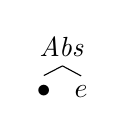
\begin{tikzpicture}[level distance=1.5em] \Tree [ .$\mathit{Abs}$ $\bullet$ $e$ ]\end{tikzpicture}\end{array}
    \cmid \begin{array}{@{}c@{}} 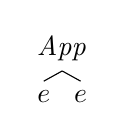
\begin{tikzpicture}[level distance=1.7em] \Tree [ .$\mathit{App}$ $e$ $e$ ]\end{tikzpicture}\end{array}\\
    \mathrm{Index} \quad
    &\iota \ &\in \quad &\mathbb{N}
    \end{alignat*}
    \vspace{-1.5em}
    \caption{The syntax of the lambda calculus}
    \label{chap4:reasoning:lambda}
\end{figure}

Firstly, in figure~\ref{chap4:reasoning:lambda}, we provide an encoding of the lambda calculus with de Bruijn indices using the expression tree structure we introduced, which takes the form of either a $\mathit{Leaf}$ or a node $\begin{array}{@{}c@{}} 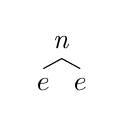
\begin{tikzpicture}[level distance=1.5em] \Tree [ .$\mathit{n}$ $e$ $e$ ]\end{tikzpicture}\end{array}$. Specifically, we encode an $\mathit{Id}$ expression (a de Bruijn index) as a $\mathit{Leaf}$ and both an abstraction and an application as nodes.
Then we encode beta reduction and eta reduction as two atomic strategies:
\begin{align*}
    &\mathit{beta}: \begin{array}{@{}c@{}}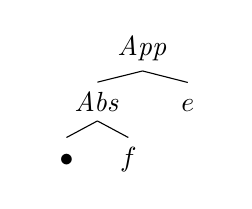
\begin{tikzpicture}[level distance=2em] \Tree [ .$\mathit{App}$ [ .$\mathit{Abs}$ $\phantom{f}\bullet\phantom{f}$ $f$ ] $\phantom{A}e\phantom{A}$ ]\end{tikzpicture}\end{array} \rightsquigarrow f [e / 0]
    &\mathit{eta}: \begin{array}{@{}c@{}}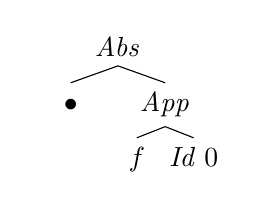
\begin{tikzpicture}[level distance=2em] \Tree [ .$\mathit{Abs}$ $\phantom{A}\bullet\phantom{A}$ [ .$\mathit{App}$ $f$ $\mathit{Id}\;0$ ]  ]\end{tikzpicture}\end{array} \rightsquigarrow f \downspoon_0
\end{align*}
where $f[e/0]$ is the de Bruijn substitution of the index $0$ with the expression $e$ in $f$ and $f \downspoon_0$ is the  de Bruijn down shifting eliminating the index $0$ in $f$.

Next we introduce the weakest precondition formula for the strategy $\mathit{normalise}(s)$, which is calculated using the weakest precondition formulae of $\mathit{repeat}(s)$ (introduced in section~\ref{chap4:reasoning:termintation}) and $\mathit{topDown}(s)$. Recall that in section~\ref{chap4:syntax} the strategy $\mathit{topDown}(s)$ is defined using the left choice combinator, the traversal $\mathit{one}(s)$ as well as the fixed-point~operator:
\[\mathit{topDown}(s) = \mu X. (s \lchoice \mathit{one}(X))\]
We can derive its weakest must succeed precondition and weakest may error precondition formulae:
\begin{align*}
    &wp_{\zeta \Vdash \mathit{topDown}(s)@l}(P) = [\text{LFP}\, \mathscr{X} : \Delta] \;l\;P
    \quad\quad\quad wp_{\zeta \Vdash \mathit{topDown}(s) @l}^\uparrow(P) = [\text{LFP}\, \mathscr{Y} : \Delta]\;l\;P\\
    &\text{\textbf{Where}:}\\
    &\Delta =
    \begin{cases}
        \mathscr{X}\,l\,P &= wp_{\zeta[(X, \cdot) \mapsto \mathscr{X} \sep (X, \uparrow) \mapsto \mathscr{Y}]\Vdash s@l}(P) \cup (wp_{\zeta[(X, \cdot) \mapsto \mathscr{X} \sep (X, \uparrow) \mapsto \mathscr{Y}] \Vdash s@l}^\uparrow (P) \\&\cap\, ((\mathscr{Y}(l\triangleright \mathscr{l})\,P \cap \mathscr{X}(l \triangleright \mathscr{r})\,P) \cup (\mathscr{Y}(l\triangleright \mathscr{r})\,P \cap \mathscr{X}(l \triangleright \mathscr{l})\,P)))\\
        \mathscr{Y}\,l\,P &= wp_{\zeta[(X, \cdot) \mapsto \mathscr{X} \sep (X, \uparrow) \mapsto \mathscr{Y}]\Vdash s@l}(P) \cup (wp_{\zeta[(X, \cdot) \mapsto \mathscr{X} \sep (X, \uparrow) \mapsto \mathscr{Y}]\Vdash s@l}^\uparrow (P) \\&\cap\, (\mathscr{Y} (l \triangleright \mathscr{l})\,P \cap \mathscr{Y} (l \triangleright \mathscr{r})\,P))
    \end{cases}
\end{align*}
With the weakest precondition formulae for $\mathit{topDown}(s)$ defined, we can subsequently  provide the weakest precondition formula for the strategy $\mathit{normalise}(s)$. Note that its weakest must succeed precondition and weakest may error precondition share the same formula, just like $\mathit{repeat}(s)$:
\begin{align*}
    &wp_{\zeta\Vdash\mathit{normalise}(s)@l}(P) = wp_{\zeta\Vdash\mathit{normalise}(s)@l}^\uparrow\zeta(P) = [\text{LFP}\, \mathscr{X}_r: \Delta_r]\,l\,P\\
    &\textbf{Where:}\\
    &\Delta_r = \mathscr{X}_r\,l\,P = [\text{LFP}\, \mathscr{X}_t : \Delta_t]\,l\,P \cup (([\text{LFP}\, \mathscr{Y}_t : \Delta_t] \,l\,P) \cap P)
\end{align*}
\begin{align*}
    &\Delta_t =
    \begin{cases}
      \mathscr{X}_t\,l\,P &= wp_{\zeta[(X, \cdot) \mapsto \mathscr{X}_r \sep (X, \uparrow) \mapsto \mathscr{X}_r \sep (Y,\cdot) \mapsto \mathscr{X}_t \sep (Y, \uparrow) \mapsto \mathscr{Y}_t]\Vdash s@l}(\mathscr{X}_r\,l\,P)
      \\&\cup\, (wp_{\zeta[(X, \cdot) \mapsto \mathscr{X}_r \sep (X,\uparrow) \mapsto \mathscr{X}_r \sep (Y, \cdot) \mapsto \mathscr{X}_t \sep (Y, \uparrow) \mapsto \mathscr{Y}_t]\Vdash s@l}^\uparrow(\mathscr{X}_r\,l\,P)
      \\&\cap\, ((\mathscr{Y}_t(l\triangleright \mathscr{l})\,P \cap \mathscr{X}_t(l \triangleright \mathscr{r})\,P) \cup (\mathscr{Y}_t(l\triangleright \mathscr{r})\,P \cap \mathscr{X}_t(l \triangleright \mathscr{l})\,P)))\\
      \mathscr{Y}_t\,l\,P &= wp_{\zeta[(X, \cdot) \mapsto \mathscr{X}_r \sep (X, \uparrow) \mapsto \mathscr{X}_r \sep (Y, \cdot) \mapsto \mathscr{X}_t \sep (Y, \uparrow) \mapsto \mathscr{Y}_t]\Vdash s@l}(\mathscr{X}_r\,l\,P)
      \\&\cup\, (wp_{\zeta[(X, \cdot) \mapsto \mathscr{X}_r \sep (X, \uparrow) \mapsto \mathscr{X}_r \sep (Y, \cdot) \mapsto \mathscr{X}_t \sep (Y, \uparrow) \mapsto \mathscr{Y}_t]\Vdash s@l}^\uparrow(\mathscr{X}_r\,l\,P)
      \\&\cap\, (\mathscr{Y}_t (l \triangleright \mathscr{l})\,P \cap \mathscr{Y}_t (l \triangleright \mathscr{r})\,P))
    \end{cases}
\end{align*}
With the weakest precondition formula for $\mathit{normalise}(s)$, we can first conclude that the strategy $\mathit{BENF}$ for calculating the $\beta\eta$-normal form for expressions is a good strategy by showing:
\[wp_{\zeta\Vdash\mathit{BENF}@l} (\mathbb{E}) \neq \emptyset\]
Although the strategy $\mathit{BENF}$ is good, some expressions are not able to be rewritten by it to a $\beta\eta$-normal form. For instance, the expression $\Omega$ is defined as:
\[\Omega \metaDef \begin{array}{@{}c@{}}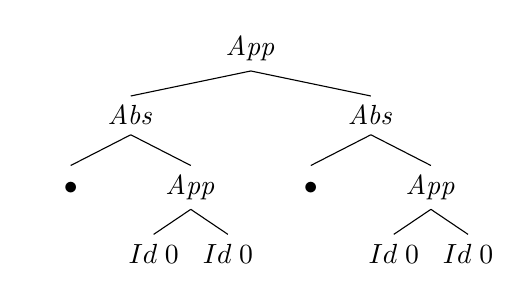
\begin{tikzpicture}[level distance=2.5em] \Tree [ .$\mathit{App}$ [ .$\mathit{Abs}$ $\phantom{A}\bullet\phantom{A}$ [ .$\mathit{App}$ $Id\;0$ $Id\;0$ ]  ] [ .$\mathit{Abs}$ $\phantom{A}\bullet\phantom{A}$ [ .$\mathit{App}$ $Id\;0$ $Id\;0$ ] ] ]\end{tikzpicture}\end{array}\]
Applying the strategy $\mathit{BENF}$ to the expression $\Omega$ will diverge, namely, the execution of the strategy $\mathit{BENF}$ on $\Omega$ is unsuccessful. We draw this conclusion by showing that $\Omega$ is not an expression in the weakest must succeed precondition of $\mathit{BENF}$\, no matter what the postcondition is:
\[\Omega \notin wp_{\zeta\Vdash\mathit{BENF}@\epsilon} (\mathbb{E}) \]
We prove this proposition straightforwardly using Scott induction.

Beside identifying expressions that fail to be normalised into a $\beta\eta$-normal form using $\mathit{BENF}$, we are also interested in examining whether a complex expression is indeed rewritten into a $\beta\eta$-normal form after applying the strategy $\mathit{BENF}$. For instance, given an expression $e$ defined as:
\[e \metaDef \begin{array}{@{}c@{}}\begin{tikzpicture}[scale=1.0, level distance=2.5em] \Tree [ .$\mathit{App}$ [ .$\mathit{Abs}$ $\phantom{A}\bullet\phantom{A}$ [ .$\mathit{Abs}$ $\phantom{A}\bullet\phantom{A}$ [ .$\mathit{Abs}$ $\phantom{A}\bullet\phantom{A}$ [ .$\mathit{App}$ $Id\;1$ [ .$\mathit{App}$ [ .$\mathit{App}$ $Id\;2$ $Id\;1$ ] $Id\;0$ ] ]  ]  ]  ] [ .$\mathit{Abs}$ $\phantom{A}\bullet\phantom{A}$ [ .$\mathit{Abs}$ $\phantom{A}\bullet\phantom{A}$ [ .$\mathit{App}$ $Id\;1$ $Id\;0$ ] ] ] ]\end{tikzpicture}\end{array}\]
we show that applying the strategy $\mathit{BENF}$ to the expression $e$ does rewrite it to a $\beta\eta$-normal form by showing the proposition below holds:
\[e \in wp_{\zeta\Vdash\mathit{BENF}@\epsilon} (\{e \barr \mathit{isBENF}\; e\})\]
The proof of this proposition is also straightforward, merely requiring the repeated unfolding of fixed-point operators.
On the basis of this result, we can conclude that the strategy $\mathit{BENF}$ performs the rewrite on the input expression $e$ as we expected, namely, rewriting $e$ into its $\beta\eta$-normal form.

\subsection{Discussion}
As this section demonstrates, our formal calculus provides precise description of strategies, independent of their length and complexity. It also provides a good characterisation of desired properties to be satisfied after the execution of a strategy, as well as of expressions that can be successfully rewritten. Additionally, our calculus is capable of performing non-trivial reasoning about rewrite strategies.
Specifically, the reasoning about beta-eta normalisation already features strategy combinators, traversals and recursion: the fundamental ingredients of strategic rewriting.
As our framework is fully mechanised in Isabelle/HOL, reasoning can be performed directly in and facilitated by the proof assistant.
Therefore, it is conceivable --- still with a significant effort --- to use our framework for reasoning about complex applications, including Elevate \citep{DBLP:journals/pacmpl/HagedornLKQGS20} compiler optimisations.
A significant initial hurdle is to encode the language that is rewritten (e.g.\ the lambda calculus in section~\ref{chap4:reasoning:beta-eta}) as well as application-specific rewrites in Isabelle/HOL, before we can start reasoning about the behaviour of more complex rewrite strategies.
With our formal calculus and its Isabelle/HOL implementation it would be possible to build up a library of standard languages and rewrites, to facilitate reasoning about increasingly complex practical applications.

\section{Related Work}
\label{related-work}
\paragraph*{Strategic Rewriting and Traversals}
Term rewriting systems~\citep{DBLP:journals/iandc/Dershowitz85} are a powerful and versatile method to express syntactic transformations. Strategic rewriting languages, which give programmers control over the rewriting process, have seen applications in many areas. Initial efforts, such as the language ELAN \citep{DBLP:journals/entcs/BorovanskyKKMV96}, focused on using rewriting as a way to model deduction and computation. The previously mentioned Stratego~\citep{DBLP:conf/icfp/VisserBT98,10.1007/3-540-45127-7_27, DBLP:journals/scp/BravenboerKVV08}, which uses System S as its core language, is designed for developing language interpreters in the Spoofax Language Workbench~\citep{DBLP:journals/software/WachsmuthKV14}.
Elevate~\citep{DBLP:journals/cacm/HagedornLKQGS23,DBLP:journals/pacmpl/HagedornLKQGS20} is very much in the style of Stratego, but is instead targeted towards guiding optimisations in a compiler for high performance computing. The language TL~\citep{DBLP:journals/scp/WinterS04} applies strategic rewriting to data processing tasks, and Strafunski~\citep{DBLP:conf/rule/LammelV02}, which is again a Stratego-like language, uses strategies for datatype-generic programming. Traversals are an essential feature of System S that also appear in other program transformation designs, such as the `Scrap your boilerplate' (SYB) style traversals (e.g. \texttt{everywhere}, \texttt{everything}, \texttt{anyDescendant}, \texttt{anyAncestor} etc.) for XML programming~\citep{10.1145/1190216.1190240}. Reachability constraints are added to types of these traversals for detecting queries that result in an empty set and transformations that always fail or do not change anything. To analyse strategic programs some algebraic laws are discussed by \citet{10.1145/1244381.1244385} for equational reasoning and by \citet{lammel2013programming} as hints of potential dead code. One could potentially make use of our weakest precondition calculus to prove and generalise these laws.

\paragraph*{Weakest Preconditions}
Weakest preconditions were introduced by Dijkstra~\citep{DBLP:journals/cacm/Dijkstra75}. \citet{DBLP:conf/rex/BonsangueK92} extend Dijkstra's calculus to include recursion in the same way that we do. Weakest preconditions are key to Cook's proof~\citep{DBLP:journals/siamcomp/Cook78} of the relative completeness of Floyd-Hoare Logic~\citep{Floyd1967,DBLP:journals/cacm/Hoare69}, and are similarly used by \citet{DBLP:conf/lics/GoncharovS13} to show relative completeness of their Hoare Logic for programs with monadic effects. \citet{DBLP:books/daglib/0073499} uses weakest preconditions as the semantic foundation for his refinement calculus, enabling stepwise derivation of programs from their specifications. In recent work, \citet{DBLP:journals/mscs/AguirreKK22} explore the categorical structure of compositional weakest preconditions, characterising them as those that are obtained from the Cartesian lifting of some monad.
As a related application of weakest preconditions, \citet{10.1145/3341707} provide a weakest prediction semantics for effectful programs, accounting for exceptions, state, non-determinism and general recursion. Their work could possibly be an alternative approach to achieve some of the goals of our work, although the application of such a formalism to the form of rewriting in formalisms like system S is not immediate. For example, it is unclear whether System S with its handling of errors and non-termination would actually form a monad. Errors alone can, of course, be handled by the Error monad; the interaction with divergence and errors is more sophisticated. As a consequence, this may give rise to complications of a similar order of magnitude as the ones addressed in this paper.

\paragraph*{Existing Formalisation and Verification}
We are not the first to examine strategic rewriting languages formally. Both the initial paper on Stratego~\citep{DBLP:conf/icfp/VisserBT98} and the paper on System S~\citep{VISSER1998422} present big-step operational semantics. However these semantics do not model divergence, and are not the basis for any formal claims. In this work, by contrast, we model all possible outcomes including divergence denotationally, and we show the denotational model equivalent to an extended big-step operational semantics of System S that includes divergence, by establishing the computational soundness and adequacy with respect to the extended big-step operational semantics. \citet{DBLP:conf/ppdp/KaiserL09} formalise a subset of System S without divergence in Isabelle/HOL by shallow embedding, but this formalisation does not include the general fixed-point operator of System S, and the choice to use shallow embedding, while convenient for some tasks, precludes the formalisation of general, meta-theoretic properties about all strategies. In our formalisation, we opt for a deep embedding, enabling us to mechanise all of the definitions and proofs in this paper. Focusing on traversals in strategic languages, \citet{lammel2013programming} characterise a list of strategic programming errors and discuss ways to avoid these errors with static typing and static analysis. With a different approach, we provide a general and formal characterisation of ``good" and ``bad" strategies as well as successful and unsuccessful executions of strategies, using our location-based weakest precondition~calculus.

\citet{KIEBURTZ2001138}, an inspiration for this work, informally sketches some weakest precondition rules for Stratego. Rather than a location-based weakest precondition calculus such as ours, \citet{KIEBURTZ2001138} includes assertions in modal logic (specifically a combination of CTL and the modal $\mu$-calculus), where the various tree modalities allow movement to different sub-expressions.
However, this modal logic variant does not have the expressive power of our framework because of our choice of location language. For instance, CTL is not expressive enough to reason about the one operator. When it comes to traversals, \citet{KIEBURTZ2001138} does not define general predicate transformers for modal assertions, and thus \citepos{KIEBURTZ2001138} rules do not form a complete calculus. It is not clear how \citepos{KIEBURTZ2001138} approach could be extended to handle traversals in their full generality.
In our work, our assertions are just sets of expressions, and we move around an expression by associating locations to our weakest preconditions. This enables us to define general rules for traversals, allowing a compositional and complete calculus for all strategies and all postconditions.
In addition, the fixed-point operator is not well constructed in \citepos{KIEBURTZ2001138} work and it is not proven to be monotone, whereas we have a correct treatment of the fixed-point operator and have proven monotonicity of all our formulae. Also, in \citepos{KIEBURTZ2001138} work, soundness is not proven, whereas we prove the soundness of our weakest precondition calculus w.r.t. the formal semantics. Lastly, we provide a careful treatment of divergence with mutually defined $\mathit{wp}$ and $\mathit{wp}^\uparrow$, while such a feature is not reflected in \citepos{KIEBURTZ2001138} work.

\paragraph*{Type Systems for Strategic Rewriting Languages} A related but parallel strand of work is in giving \emph{types} to strategic rewriting languages. \citet{DBLP:conf/sle/SmitsV20} add gradual typing to Stratego and use it to find bugs in their strategies for language interpreters. \citet{DBLP:conf/birthday/Koppel23} uses typed strategies to model multi-language program transformations, \citet{DBLP:journals/jlp/Lammel03} adds types to strategies with applications to generic programming in typed languages and \citet{fu2023traced} makes use of structural typing with traces for checking ill-composed strategies statically. These type systems emphasise lightweight static or the hybrid of dynamic and static checking to find bugs, whereas our focus is on a complete semantic accounting of rewriting strategies, and the development of a weakest precondition calculus that can demonstrate the absence of bugs, not merely their presence.

\paragraph*{Kleene Algebra}
Strategic rewriting languages resemble a Kleene Algebra~\citep{DBLP:conf/lics/Kozen91} extended with traversals and a biased choice operator. There have been many other extensions to Kleene Algebra, most notably Concurrent Kleene Algebra~\citep{DBLP:journals/jlp/HoareMSW11}, which adds parallel composition, and Kleene Algebra with Tests~\citep{DBLP:journals/toplas/Kozen97}, which adds Boolean guards to model the semantics of \textbf{while} programs. \citet{DBLP:conf/lics/Kozen99} shows that  reasoning by Kleene Algebra with Tests entirely subsumes Hoare Logic for \textbf{while} programs. A version of Kleene Algebra with Tests, NetKAT, has been used to reason about packet switching networks~\citep{DBLP:conf/popl/AndersonFGJKSW14}. Recently, Concurrent Kleene Algebra and NetKAT have been combined for reasoning about concurrent network systems~\citep{DBLP:conf/esop/WagemakerFKKRS22}.

\paragraph*{Denotational semantics and adequacy}
\;The appeal of the Scott-Strachey approach to
semantics \citep{stoy1985denotational} is in its local and
compositional reasoning, and over the last $50$ years it has been used
for many diverse programming languages. As far as programming language
abstractions go, the strategic rewriting language we consider is mostly standard,
and we were able to use the following relevant semantic tools with
relatively minor modification. \citeauthor{plotkin:powerdomain}
pioneered the powerdomain construction
\citeyearpar{plotkin:powerdomain} and later characterised it as the
free semilattice over a
domain~\citep{hennessy-plotkin:plotkin-powerdomain}. Most denotational
accounts include an adequacy proof, and it is possible to prove them
wholesale for standard programming languages with a myriad of
expressive
features~\citep{SIMPSON2004207,plotkin-power:adequacy,johann-simpson-voigtlander:adequady}.
We found the decomposition of computational adequacy into dual
inductive and coinductive arguments interesting, and we hope it could
inform other reflective accounts of
adequacy~\citep{campos-levy:adequacy}.

\section{Conclusion and Future Work}
\label{chap4:conclusion-future-work}
We have presented Shoggoth, a rigorous formal foundation for strategic rewriting languages, including a comprehensive semantic accounting of System S, and a weakest precondition calculus to facilitate formal reasoning about rewriting strategies. Our semantic treatment models all possible executions of strategies including divergences in both denotational and big-step operational models, and our proofs of soundness and adequacy demonstrate the equivalence of these models. Our location-based weakest precondition calculus is the first formal axiomatic treatment of rewriting strategies, and enables reasoning about traversals by having the notion of location for indicating where in an expression a given strategy operates. Our soundness proof justifies our location-based weakest precondition calculus with respect to our semantic models, and we demonstrate practical application of this calculus by applying it to realistic examples. All of our work has been mechanised in over 5,000 lines of Isabelle/HOL proof script.

Weakest precondition calculi form the basis of \emph{verification condition generators} (VCGs), which are a key component of many automatic and semi-automatic verification tools such as VCC~\citep{DBLP:conf/tphol/CohenDHLMSST09} and Dafny~\citep{DBLP:conf/lpar/Leino10}, as well as of static analysers such as the popular Extended Static Checking extension for Java~\citep{DBLP:conf/pldi/FlanaganLLNSS02, DBLP:journals/ipl/Leino05}. We envision that our weakest precondition calculus could similarly inform the design of a VCG for automatic verification or static checking of rewriting strategies. We intend to use Shoggoth as a foundation for the development of tools for verification and, potentially, \emph{synthesis} of rewriting strategies.

\noindent
\begin{center}
\vspace{0.3em}

\begin{tikzpicture}[color=black,
                   transform shape,
                   every node/.style={inner sep=0pt}]
\node[minimum width=0.35\framesize, minimum height=0.05*\framesize, fill=white](vecbox){};
\node[anchor=west] at (vecbox.west){\pgfornament[width=0.08*\framesize]{16}};
\node[anchor=east] at (vecbox.east){\pgfornament[width=0.08*\framesize]{15}};
\node[inner sep=6pt] (text) at (vecbox.center){\textbf{\Large Epilogue}};
\end{tikzpicture}
\vspace{-0.3em}
\end{center}
% \section{Epilogue}
% \label{chap4:epilogue}
In this study, we have analysed and designed a reasoning framework for syntactic transformations and their compositions via processing their formal semantics. In the end, I would like to enclose this chapter again with some high-level observations and a reflection.

In a strategic rewriting system, the syntax of manipulating expressions and semantics which is the evaluation of expressions are interdependent. Since the syntactic transformations of expressions encode the process of evaluating the semantics of these expressions and by composing these syntactic transformation steps, we have the syntax of a strategic rewriting language, providing a concise abstractions interface to not only compose but also control the application of these strategies. Again, by analysing the semantics of such syntax for composing strategies, we are able to understand and reason about the execution of these compositions of syntactic transformations. One may find such an process of detailed analysis of some concise language constructions for syntactic transformations against the intuition of reasoning about programs --- normally people utilise some notions like type systems and logic formulae which are more abstract than the encoding of these programs. However, I find it is hard to design some constructs which are even more abstract than the existing syntax of these compositions for reasoning about there executions, rather, the behaviours hidden beneath the syntactic constructs of these compositions are surprisingly complicated and can only be properly assessed by modelling their executions. 

In modelling the semantics of System S, there is again a trade-off between concise abstractions and precise expressiveness. To be able to see the composition of strategies clearly, we simplified our understanding of atomic strategies, abstracting their implementation complex details by modelling them as partial functions. With such an abstraction, some computation details of these atomic strategies are not considered like the side effects of the execution of an atomic strategy. However, by doing so we are able to concentrate on what possible results they can produce contributing to the analysis of the compositions rather than how they get evaluated to produce these results, allowing us to separate the process of semantic analysis of the composition of strategies from the detailed constructions of the expressions to be rewritten, thus making the semantics and reasoning framework we have build more general.


% Back to the relationship of syntax and semantics of programming languages, in this small study, the syntax and semantics are interdependent since we have observed that the transformations of the syntax of expressions encode the meaning for the evaluation of these expressions, and we can characterise and reason about the executions of compositions of these syntactic transformations by assigning to and analysing of the semantics of them. Such an observation, aside of the practical usefulness of the framework Shoggoth we build enabling formal understanding and reasoning of strategic rewriting languages, is conceptually intriguing as a perspective of the study of the syntax and semantics in the design of programming languages.
\Chapter{The~Thorn~and~The~Bird:~Still~We~Do~It}{Conclusion}
\label{chap5}
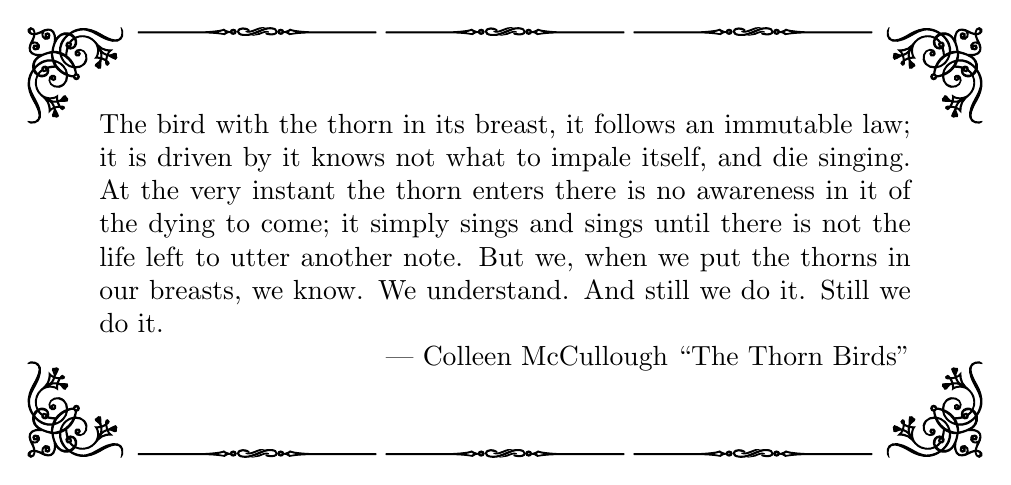
\begin{tikzpicture}[color=black,
                   transform shape,
                   every node/.style={inner sep=0pt}]
\node[minimum width=\framesize, minimum height=0.45 *\framesize, fill=white](vecbox){};
\node[anchor=north west] at (vecbox.north west){% 
\pgfornament[width=0.1*\framesize]{61}};
\node[anchor=north east] at (vecbox.north east){% 
\pgfornament[width=0.1*\framesize,symmetry=v]{61}};
\node[anchor=south west] at (vecbox.south west){% 
\pgfornament[width=0.1*\framesize,symmetry=h]{61}};
\node[anchor=south east] at (vecbox.south east){% 
\pgfornament[width=0.1*\framesize,symmetry=c]{61}};
\node[anchor=north] at (vecbox.north){% 
\pgfornament[width=0.25*\framesize]{88}
\pgfornament[width=0.25*\framesize]{88}
\pgfornament[width=0.25*\framesize]{88}
};

\node[anchor=south] at (vecbox.south){% 
\pgfornament[width=0.25*\framesize]{88}
\pgfornament[width=0.25*\framesize]{88}
\pgfornament[width=0.25*\framesize]{88}
};
\node[text width=0.85\framesize, align=justify] at (vecbox.center){%
The bird with the thorn in its breast, it follows an immutable law; it is driven by it knows not what to impale itself, and die singing. At the very instant the thorn enters there is no awareness in it of the dying to come; it simply sings and sings until there is not the life left to utter another note. But we, when we put the thorns in our breasts, we know. We understand. And still we do it. Still we do it.\\ 
\rightline{--- Colleen McCullough ``The Thorn Birds"}};
\end{tikzpicture}
% I might think about a better title
% I think this title is good enough
\lettrine{T}{hroughout} this manuscript, three conceptual questions have been addressed via three studies presented in chapter~\ref{chap2}, chapter~\ref{chap3}, and chapter~\ref{chap4}, ultimately, they all relate to the fundamental motivation of my researches concerning the meaning of computer programs --- to design better abstraction for modelling and understanding programs as well as better formal frameworks for reasoning about programs.

The study discussed in chapter~\ref{chap2} is conducted to address the first conceptual question: How to design a better abstraction mechanism that allows programmers to effectively express \emph{what} they want a computer to do via some declarative yet accurate \emph{specifications} instead of \emph{how} a computer should accomplish a task via some concrete \emph{implementations}? The study specifically focuses on designing property-based container types in programming languages. In particular, we investigate ways to declaratively specify the properties of container types using formal specifications instead of having these properties concretely implemented for container types, allowing concrete implementations to be inferred from the specifications. In this study, we utilise existing verification techniques including formal specifications, data refinement, and refinement types for the purpose of designing declarative yet accurate abstractions. We demonstrate that these specifications describing \emph{what} properties, especially properties giving an account of functional requirements that a container type and its operations should satisfy, which are separated from concrete container implementations describing \emph{how} properties are satisfied. In terms of addressing the conceptual question regarding to the understanding of the relationship between specifications and implementations, the design of property based container types in this study indicates that declarative specifications enable better automation and optimisation for application programmers when selecting desired container implementations in programs. 

The study discussed in chapter~\ref{chap3} is conducted to address the second conceptual question: How to intuitively understand \emph{distributed programs} using the same conceptual model as \emph{monolithic programs}? The study focuses on designing, implementing, and formalising a UMI framework as a Rust library. This UMI framework allows a distributed program to be migrated a monolithic program without massive changes to the syntax or structure of the original monolithic program. In addition, the semantics of the monolithic program is preserved. By formalising the core calculus of the UMI framework implemented as a distributed extension of Rust, we argue that our UMI framework extends Rust's memory safety guarantees into a distributed setting by utilising Rust's ownership and lifetime system in distributed memory management. In terms of addressing the conceptual question regarding to understanding the connection between monolithic programs and distributed programs, the UMI framework demonstrates that a monolithic program can be viewed as an abstraction of a distributed program. Rather than requiring programmers to implement \emph{how} some functionalities are achieved in a distributed setting via network communication protocols and message passing, programmers only need to specify \emph{what} these functionalities a distributed program is required to achieve in terms of a monolithic program by abstracting away the details of distributed memory management and message passing over a network.

The study discussed in chapter~\ref{chap4} is conducted to address the third conceptual question: How do we characterise the relationship between the \emph{syntax} and \emph{semantics} of programming languages? The study focuses on a thorough examination of the semantics of a core calculus --- System S --- of a family of strategic rewriting languages that instructs syntactic transformations. More specifically, we formalise a denotational semantics and big-step operational semantics of System S, featuring errors, divergence, and non-determinism. In addition, we prove the equivalence of these two semantic models, showing that they are equally expressive, and model the same meaning of System S. We then present an axiomatic model of System S, which is a weakest precondition calculus, allowing us to reason about the executions of rewrites encoded in System S. Regarding to the conceptual question, this study demonstrate a perhaps interesting observation: As for strategic rewriting languages, the syntax and semantics are interdependent. The syntactic transformations of expressions encode the meaning for the evaluation of these expressions, and by designing and analysing three different formal models of semantics, we are able to characterise and reason about the executions of compositions of these syntactic transformations.

% With respect to the theme of this manuscript --- studies concerning the meaning of computer programs, 
There is one important observation shared by all three studies: There is always a trade-off between the expressiveness and the elegance of abstraction when modelling programming languages. In the first study, we have observed that it is challenging to express performance related non-functional properties for containers using the declarative formal specification we have designed. In the second project, we have presented our UMI framework which provides a conceptual modelling which views a monolithic program as a functional specification of a distributed program, abstracting over the complicated network communication details while extending the memory safety guarantees provided by the monolithic program into a the distributed program. However, such an abstraction is not expressive enough to capture the failures caused by the network communication problems and server errors. In the third project, in order to formalise concise and elegant semantics of the composition of syntactic transformations, we abstract away the detail implementations of the atomic strategies and model them as partial functions. However, such an abstraction is not expressive enough to model concepts such as side effects of the execution of atomic strategies. To summarise such an observation, ff the model is too detailed and precise, it may become overly specific and complicated, lose the generality, and obscure the high-level structure of the language features that it models. However, if the model if too abstract, it may lose the some important aspects of the language features that it models. When we are designing a formal model to demonstrate some principled understanding of some features we care in a programming language, we should always take the balancing between expressiveness and abstraction into consideration. 

Back to the theme of this manuscript --- studies concerning the meaning of computer programs, we have conducted three studies relating to explore better techniques for modelling important features and components of programming languages, including container types, distributed programming, and term rewriting. These studies enable programmers to gain formal understanding of computer programs, to effectively communicate desired functionalities to computers without being overly specific, and to reason about the executions of computer programs. 

\begin{center}
\vspace{-0.7em}
\pgfornament[width=0.08*\framesize]{11}
\pgfornament[width=0.08*\framesize]{80}
\pgfornament[width=0.08*\framesize]{14}
\vspace{-0.3em}
\end{center}

Everything beautiful will eventually come to an end. Although I have been asking different questions, wondering around different paths, and searching for different angles to gain some understandings of the questions I have been asking, like the bird with the impaling thorn, everything I have been exploring eventually leads to the same direction: I am in the process of searching for the meaning of the world, especially the world of which I am the centre --- and in the end the result might just be: \emph{It is meaningless}. Nevertheless, I know, I understand, even if there is nothing there, still I search for it, till the end of my life, still I search for it.
% \chapter{Specifications, All Too Specific}
\label{chap2}
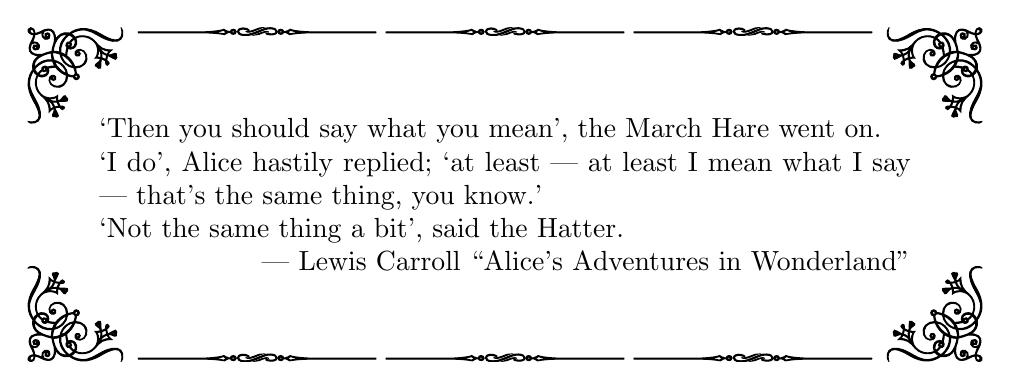
\begin{tikzpicture}[color=black,
                   transform shape,
                   every node/.style={inner sep=0pt}]
% \node[minimum size=\framesize,fill=white](vecbox){};
% \node[text width=\framesize,align=center](Text){%
%     `Then you should encode what you mean', the March Hare went on.
% \\
% `I do', Programmer hastily replied; `at least --- at least I mean what I encode --- that's the same thing, you know.'
% \\
% `Not the same thing a bit', said the Hatter.};
\node[minimum width=\framesize, minimum height=0.35 *\framesize, fill=white](vecbox){};
\node[anchor=north west] at (vecbox.north west){% 
\pgfornament[width=0.1*\framesize]{61}};
\node[anchor=north east] at (vecbox.north east){% 
\pgfornament[width=0.1*\framesize,symmetry=v]{61}};
\node[anchor=south west] at (vecbox.south west){% 
\pgfornament[width=0.1*\framesize,symmetry=h]{61}};
\node[anchor=south east] at (vecbox.south east){% 
\pgfornament[width=0.1*\framesize,symmetry=c]{61}};
\node[anchor=north] at (vecbox.north){% 
\pgfornament[width=0.25*\framesize]{88}
% \pgfornament[width=0.1*\framesize]{15}
% \pgfornament[width=0.1*\framesize]{16}
\pgfornament[width=0.25*\framesize]{88}
\pgfornament[width=0.25*\framesize]{88}
};

\node[anchor=south] at (vecbox.south){% 
% \pgfornament[width=0.25*\framesize]{88}
% \pgfornament[width=0.1*\framesize,symmetry=h]{15}
\pgfornament[width=0.25*\framesize]{88}
\pgfornament[width=0.25*\framesize]{88}
\pgfornament[width=0.25*\framesize]{88}
% \pgfornament[width=0.1*\framesize,symmetry=h]{16}
% \pgfornament[width=0.25*\framesize]{88}
};
% \node[anchor=south] at (vecbox.south){% 
% \pgfornament[width=0.6*\framesize]{46}};
% \node[anchor=north,rotate=90] at (vecbox.west){% 
% \pgfornament[width=0.6*\framesize,symmetry=h]{46}};
% \node[anchor=north,rotate=-90] at (vecbox.east){% 
% \pgfornament[width=0.6*\framesize,symmetry=h]{46}};
\node[text width=0.85\framesize,align=justify] at (vecbox.center){%
% `Then you should \emph{encode} what you mean', the March Hare went on.
% \\
% `I do', \emph{Programmer} hastily replied; `at least --- at least I mean what I \emph{encode} --- that's the same thing, you know.'
% \\
% `Not the same thing a bit', said the Hatter.\\
% \rightline{--- \emph{Altered} Alice's Adventures in Wonderland}};
% \node[text width=0.85\framesize,align=right] at (vecbox.south){%
%    --- \emph{Altered} Alice's Adventures in Wonderland};
`Then you should say what you mean', the March Hare went on.
\\
`I do', Alice hastily replied; `at least --- at least I mean what I say --- that's the same thing, you know.'
\\
`Not the same thing a bit', said the Hatter.\\
\rightline{--- Lewis Carroll ``Alice's Adventures in Wonderland"}};
\end{tikzpicture}
\section{Prologue}
\label{chap2:prologue}
People often try to \emph{say} what they \emph{mean}, however, there is always a gap between what they say and what they really mean --- \emph{they do not mean what they say.} Likewise, programmers often try to \emph{encode} what they \emph{meant for} a computer to do, however, there is always a gap between what they encode and what they really want a computer to execute --- \emph{they do not mean what they encode.}

One observation is that in an implementation of an application, what an application developer encode tends to be ``all too specific" comparing to what they have modelled in mind.
% One issue we intend to look into in this project is that encoding of container types in an application being ``all too specific". 
Take a container type example which is illustrated in later sections, when an application developer wants to use a \emph{unique container} in an application, the application developer \emph{means} that the container does not contain any duplicated elements. However, the application developer often has to \emph{encode} such a required container as a tree, a hash table, a list without duplicated element etc. By choosing a concrete encoding, application developers no longer just expresses what they mean, but additionally committing to certain performance characteristics or memory consumption which may not be desirable.

Hence, we would like to look into the designing a programming framework, facilitating application developers to better express what they meant for a computer to execute via writing declarative specifications instead of encoding concrete and fixed implementations. 
We believe that such a framework would also enable better automation and optimisation: It gives opportunities to a tool such as a compiler to select or generate a best performing implementation according to the specification provided by an application developer.

% To address this issue, we propose to design a framework, to allow application programmers to better express what they mean: What properties a container should have, instead of how these properties are implemented.

\section{Introduction}
\label{chap2:introduction}
Container data types, such as sets, lists, and trees, represent collections of data ubiquitous in everyday programming~\citep{DBLP:books/daglib/0023376}. Virtually all programming languages provide a variety of container implementations in their standard libraries.

Much work has been done to design better abstractions, improve performance and verify correctness for container data types.
However, a crucial problem for application developers using containers still exists:
when choosing a container data type, application developers are forced to select a concrete implementation that comes with certain theoretical complexity and practical performance tradeoffs.

% For example, let us consider a situation where an application developer would like to represent a mathematical set of elements, i.e., where each element should occur at most once in the set.
For example, consider representing a mathematical set, i.e., where each element should occur at most once.
In \Cpp, we must choose between \lstinline{std::set}, usually implemented as red-black trees~\citep{DBLP:journals/acta/Bayer72}, and \lstinline{std::unordered_set}, implemented as a hash table.
The hash-based implementation was added to the \Cpp standard in 2011, as the \Cpp standard has strict complexity requirements preventing the ordinary \lstinline{std::set} to be implemented as the (often faster) hash table.
Many blog posts and discussions~\citep{blog1,blog2,blog3,blog4,blog5} report on the performance of various \Cpp containers, showing the community's interest and the need for external guidance that the language itself does not provide.

In other languages, the situation is similar.
Rust provides two container implementations, \lstinline{HashSet} and \lstinline{BTreeSet}, expecting application developers to make an explicit choice between them.
Scala's complex collection library features abstract interfaces, such as the \lstinline{Set} trait, abstracting over many implementations such as \lstinline{HashSet} and \lstinline{TreeSet}.
But when creating an instance of \lstinline{Set}, a default \lstinline{HashSet} implementation is chosen regardless of the suitability of this implementation choice for the usage pattern of the application.

These examples demonstrate a general problem:
Application developers are forced to \emph{overspecify}, by having to select a concrete implementation, where we generally would like application developers to be shielded from low-level implementation details.
Application developers should primarily care about the \emph{abstract behaviour} of the containers in their application, and not how this is achieved.
The compiler, or a dedicated tool, should identify those containers that satisfy their functional requirements, and select the best implementation automatically.

In this paper, we propose an automated tool: \Primrose{}, which allows application developers to specify the expected behaviours and programming interfaces of containers as \emph{properties}.
\emph{Syntactic properties} specify the required programming interface of the container and are expressed as traits of the underlying programming language.
\emph{Semantic properties} specify the expected behaviour of the container and are written as logical predicates used as refinements of the container type.
\Primrose{} automatically selects the set of valid implementations for which the \emph{library specifications}, written by the library developers as pre- and post-conditions of the container operations, satisfy the specified syntactic and semantic properties using an SMT solver.
Finally, \Primrose{} ranks the valid library implementations based on 
their runtime performance.

% feels like i might be repeating something here..
To select the best container implementation, firstly, those container implementations which meet the functional requirements of the application developer must be determined, and then those valid container implementations must be evaluated based on non-functional requirements. While \Primrose{} does include functionality for ranking based on benchmarks, the focus of this paper is on the first of these two problems. There are many existing sophisticated techniques for selecting based on non-functional requirements, and they are highly complementary with \Primrose{}.

In this work, we apply verification and formal methods techniques, including refinement types, formal library specifications, and SMT solvers, in an innovative way to raise the level of abstraction for developers, freeing them from the burden of choosing container implementations, and opening up the possibility to automatically improve the performance of applications.

To summarise, this paper makes the following contributions:
\begin{itemize}
    \item We present \Primrose{} (section~\ref{chap2:overview}), a language-agnostic tool for selecting valid container implementations (section~\ref{chap2:select}) based on \emph{properties} (section~\ref{chap2:prop}) used to describe their behaviour and programming interface, and ranking them based on their performance.
    \item We show a new application of refinement types not---as previous work did---for verification purposes, but to raise the level of abstraction for developers and to improve the runtime performance of applications with container data types (section~\ref{chap2:prop}).
    \item We develop a new methodology to specify container libraries, amenable to our selection process, making use of existing formal methods work such as data abstraction and Hoare logic (section~\ref{chap2:lib}).
    \item We show the feasibility of \Primrose{}, selecting container implementations that satisfy various properties from a Rust library of eight container types with library specifications. We validate container implementations against specifications and evaluate the efficiency of the selection process (section~\ref{chap2:evaluation}).
\end{itemize}

\section{Motivation}
\label{chap2:motivation}
Suppose as part of a larger application, we want to find and store all the elements of a larger collection, but without duplicates.
We might, for example, use the result of this function to count the number of unique elements or process the elements further, now with the guarantee that each element in the returned collection is unique.

An easy way to implement this is to return a container that only permits unique elements.
We might think of a \emph{set}, however, as discussed in section~\ref{chap2:introduction}, this requires a choice:
Which concrete implementation of the abstract idea of a mathematical set should we use? 

\begin{figure}[t]
    \centering
    \begin{subfigure}[t]{0.48\textwidth}
        \centering
\begin{lstlisting}[language=Rust, style=boxed, basicstyle=\footnotesize\ttfamily,escapechar=!]
type Set<I> = HashSet<I>;!\tikzmark{figure1a}!
// type Set<I> = BTreeSet<I>;
// type Set<I> = UniqueVect<I>;
// type Set<I> = FancySetImpl<I>;
// type Set<I> = HashMultiSet<I>; ?

let mut uniqueElements 
  = Set::new();
for val in input.iter() {
    uniqueElements.insert(val);  }
\end{lstlisting}
\begin{tikzpicture}[remember picture, overlay]
    \node [right=0.8cm of figure1a,yshift=+0.075cm,
           inner sep=0.075cm] {\footnotesize\bfseries\texttt{Rust}};
\end{tikzpicture}
        \caption{In Rust, application developers must choose a concrete container implementation with potentially surprising performance implications.}
        \label{fig:motivating_example:rust}
    \end{subfigure}
    \hfill
    \begin{subfigure}[t]{0.48\textwidth}
        \centering
\begin{lstlisting}[language=Rust, style=boxed, basicstyle=\footnotesize\ttfamily]
!\tikzmark{figure1b-primrose-start}!property unique {
  \c -> (for-all-elems (\a ->
    (unique-count? a c)) c) };
type UniqueCon<I> = {
  c <: ContainerT | unique c };!\tikzmark{figure1b-primrose-end}!

let mut uniqueElements
  = UniqueCon::new();
for val in input.iter() {
    uniqueElements.insert(val);  }
\end{lstlisting}
\begin{tikzpicture}[remember picture, overlay]
    \draw   ($(figure1b-primrose-start) + (-0.05,+0.27)$)
        rectangle
            ($(figure1b-primrose-end)   + (+0.8,-0.10)$);
    \node [right=4.4cm of figure1b-primrose-start,
           yshift=+.075cm,
           inner sep=0.075cm] {\footnotesize\bfseries\texttt{Primrose}};
    \node [right=5.25cm of figure1b-primrose-start,
           yshift=-3.25cm,
           inner sep=0.075cm] {\footnotesize\bfseries\texttt{Rust}};
\end{tikzpicture}
        \caption{Using \Primrose{}, developers describe the container's expected behaviour via \emph{properties} and the best valid implementation is selected.}
        \label{fig:motivating_example:primrose}
    \end{subfigure}
    \vspace{1em}
    \caption{Selecting the unique elements of a sequence by inserting the elements into a \emph{set}.}
    \label{fig:motivating_example}
\end{figure}


Figure~\ref{fig:motivating_example:rust} shows a Rust code snippet computing a container \lstinline{uniqueElements} that contains the unique elements of the original \lstinline{input} sequence.
The application developer must choose a concrete container implementation, such as \lstinline{HashSet} in line 1, but
other valid choices would be Rust's \lstinline{BTreeSet} (line 2), or perhaps a custom \lstinline{UniqueVect} (line 3) container, which stores all elements in a vector but ensures there are no duplicates, 
or some other \lstinline{FancySetImpl}ementations (line 4). 
Whether a container implementation is \emph{valid} is determined by the application developer's \emph{functional requirements}. Our uniqueness requirement, for example, is not met by the Rust \lstinline{HashMultiSet} (line 5). 
If the application developer also required elements to be stored in a particular order, this would also rule out the \lstinline|HashSet| implementation.

Many programming techniques exist to abstract over multiple concrete implementations of a general concept.
In object-oriented languages, \emph{abstract classes} enable hiding multiple implementations behind a common interface.
Similar features exist in other languages under different names, such as, \emph{traits} (e.g., in Rust and Scala), \emph{protocols} (e.g., in Swift), \emph{interfaces} (e.g., in Java), and \emph{type classes} (e.g., in Haskell).
All these techniques allow developers to use multiple concrete implementations, such as \lstinline{HashSet} and \lstinline{BTreeSet}, with a single abstract type, which we might call \lstinline{Set}.
%Abstract types list the operations that must be supported by each concrete implementation, and the types of these operations.
However, these types are deliberately \emph{abstract}, meaning that we \emph{cannot} instantiate them directly:
When creating such a type, a developer must commit to a specific concrete implementation, requiring the developer to look underneath layers of abstraction to make an informed decision.
Thus, these abstraction techniques do not free developers from considering low level details and they are not powerful enough to express \emph{semantic} requirements:
developer cannot specify their functional requirements directly, but merely provide a common \emph{syntax} enabling the use of multiple implementations. 
With such an abstract container type \lstinline{Set}, we cannot express that each concrete implementation is required to contain no duplicate elements.
Similarly, with an abstract type \lstinline{Stack}, we cannot state that the last-in-first-out property is respected by the \lstinline{push} and \lstinline{pop} operations.

Figure~\ref{fig:motivating_example:primrose} shows the same problem of selecting unique elements, but expressed using \Primrose{}.
Application developers specify their functional requirements---in this case, that the container must contain unique elements---as a \emph{semantic property}.
This semantic property is expressed in lines 1--3 in the \Primrose{} specification language as a logical predicate written as a lambda expression.
The property is used to \emph{refine} the container data type in lines 4 and 5.
Refinement types have long been used as a technique for program verification---including container types~\citep{DBLP:conf/esop/VazouRJ13}.
Here, we use refinement types in a new way, allowing programmers to express the expected behaviour of a container, and freeing them from having to make a (potentially difficult) implementation choice.
The remaining code remains unchanged: we can simply use the refined type in line 7.
\Primrose{} preprocesses the code from figure~\ref{fig:motivating_example:primrose}, identifies all valid container implementations from a library of containers, and generates a program equivalent to figure~\ref{fig:motivating_example:rust} with the best container implementation inserted~automatically.

\begin{figure}[t]
    \centering
\small
\begin{subfigure}[t]{0.48\textwidth}
\begin{tikzpicture}
\begin{axis}[
  width=\textwidth, height=0.75\textwidth,
  xlabel=Data size (MB),
  ylabel=Time (s),
  legend style={
    at={(0.3, 0.95)},anchor=north
}]
\addplot[kirby-blue, mark=o] table [y=BTreeSet, x=Data]{insertion.dat};
\addlegendentry{\scriptsize BTreeSet}
\addplot[teal!70!white, mark=10-pointed star] table [y=HashSet, x=Data]{insertion.dat};
\addlegendentry{\scriptsize HashSet}
\addplot[kirby, mark=x] table [y=UniqueVec, x=Data]{insertion.dat};
\addlegendentry{\scriptsize UniqueVec}
\end{axis}
\end{tikzpicture}
\end{subfigure}
\hfill
\begin{subfigure}[t]{0.48\textwidth}
\begin{tikzpicture}
\begin{axis}[
  width=\textwidth, height=0.75\textwidth,
  xlabel=Data size (MB),
  ylabel=Heap allocations (MB),
  legend style={
    at={(0.3, 0.95)},anchor=north
}]
\addplot[kirby-blue, mark=o] table [y=BTreeSet, x=Data]{memory.dat};
\addlegendentry{\scriptsize BTreeSet}
\addplot[teal!70!white, mark=10-pointed star] table [y=HashSet, x=Data]{memory.dat};
\addlegendentry{\scriptsize HashSet}
\addplot[kirby, mark=x] table [y=UniqueVec, x=Data]{memory.dat};
\addlegendentry{\scriptsize UniqueVec}
\end{axis}
\end{tikzpicture}
\end{subfigure}

    \caption{Runtime performance (left) and memory consumption (right) of three container implementations for storing unique elements of an input sequence from \ref{fig:motivating_example:rust}.
    The custom \lstinline{UniqueVec} implementation ensures elements to be unique lazily on access. It is the fastest implementation, outperforming \lstinline{HashSet} and \lstinline{BTreeSet} from the Rust standard library, while consuming less memory than \lstinline{HashSet}.}
    \label{fig:motivating_graph}
\end{figure}

%\todo[author=Michel]{Are the memory consumption measurements in Figure 2 correct? Shouldn't the vector consume much less memory than the tree that requires additional pointers? Basically, I would have expected that the vector only consumes about 400 MB for 400 MB of data, but it seems to be more than 2x that!}
However, which is the \emph{best} container implementation?
This depends on the non-functional requirements of the application:
Often developers care about fast runtime performance, also, for example, an application might require a low memory footprint.
Figure~\ref{fig:motivating_graph} shows the performance and memory consumption for three different implementation choices.
Perhaps surprisingly, a custom \lstinline{UniqueVec} implementation that uses a vector and lazily ensures that the stored elements are unique, by sorting the vector and removing duplicates on access, outperforms the Rust built-in containers \lstinline{HashSet} and \lstinline{BTreeSet}. In addition, it is also the best choice for machines with limited memory.
Choosing the best container implementation is not always straightforward, particularly as theoretical complexity of operations can sometimes be misleading in the presence of practical effects such as cache-friendliness. \Primrose{} selects implementations satisfying developers' functional requirements and opens up opportunities to automatically choose the most desired implementation according to non-functional requirements. 
%Using \Primrose{}, developers do not have to worry about choosing an implementation which is incorrect, and ranking the implementations by performance helps to avoid subpar performance.
% Next, we are going to discuss an overview of the \Primrose{} tool.

\section{Overview}
\label{chap2:overview}
Figure~\ref{overview:design} gives an overview of the design of the \Primrose{} selection tool. Using \Primrose{}, the application developer writes code in terms of an abstract type, and a 
\emph{property specification} describing the syntactic and semantic properties they expect this type to satisfy. The syntactic properties take the form of traits and the semantic 
properties take the form of type refinements.
To write a program, the developer only specifies what functional properties must be satisfied by the required container, and does not have to commit to a particular 
implementation. The developer specifies that they require a container (the syntactic property \lstinline{ContainerT}) where all elements are unique (the semantic property \lstinline{unique}). We discuss properties in detail in section~\ref{chap2:prop}.

% The diagram of system here
\begin{figure}[t]
  \centering
      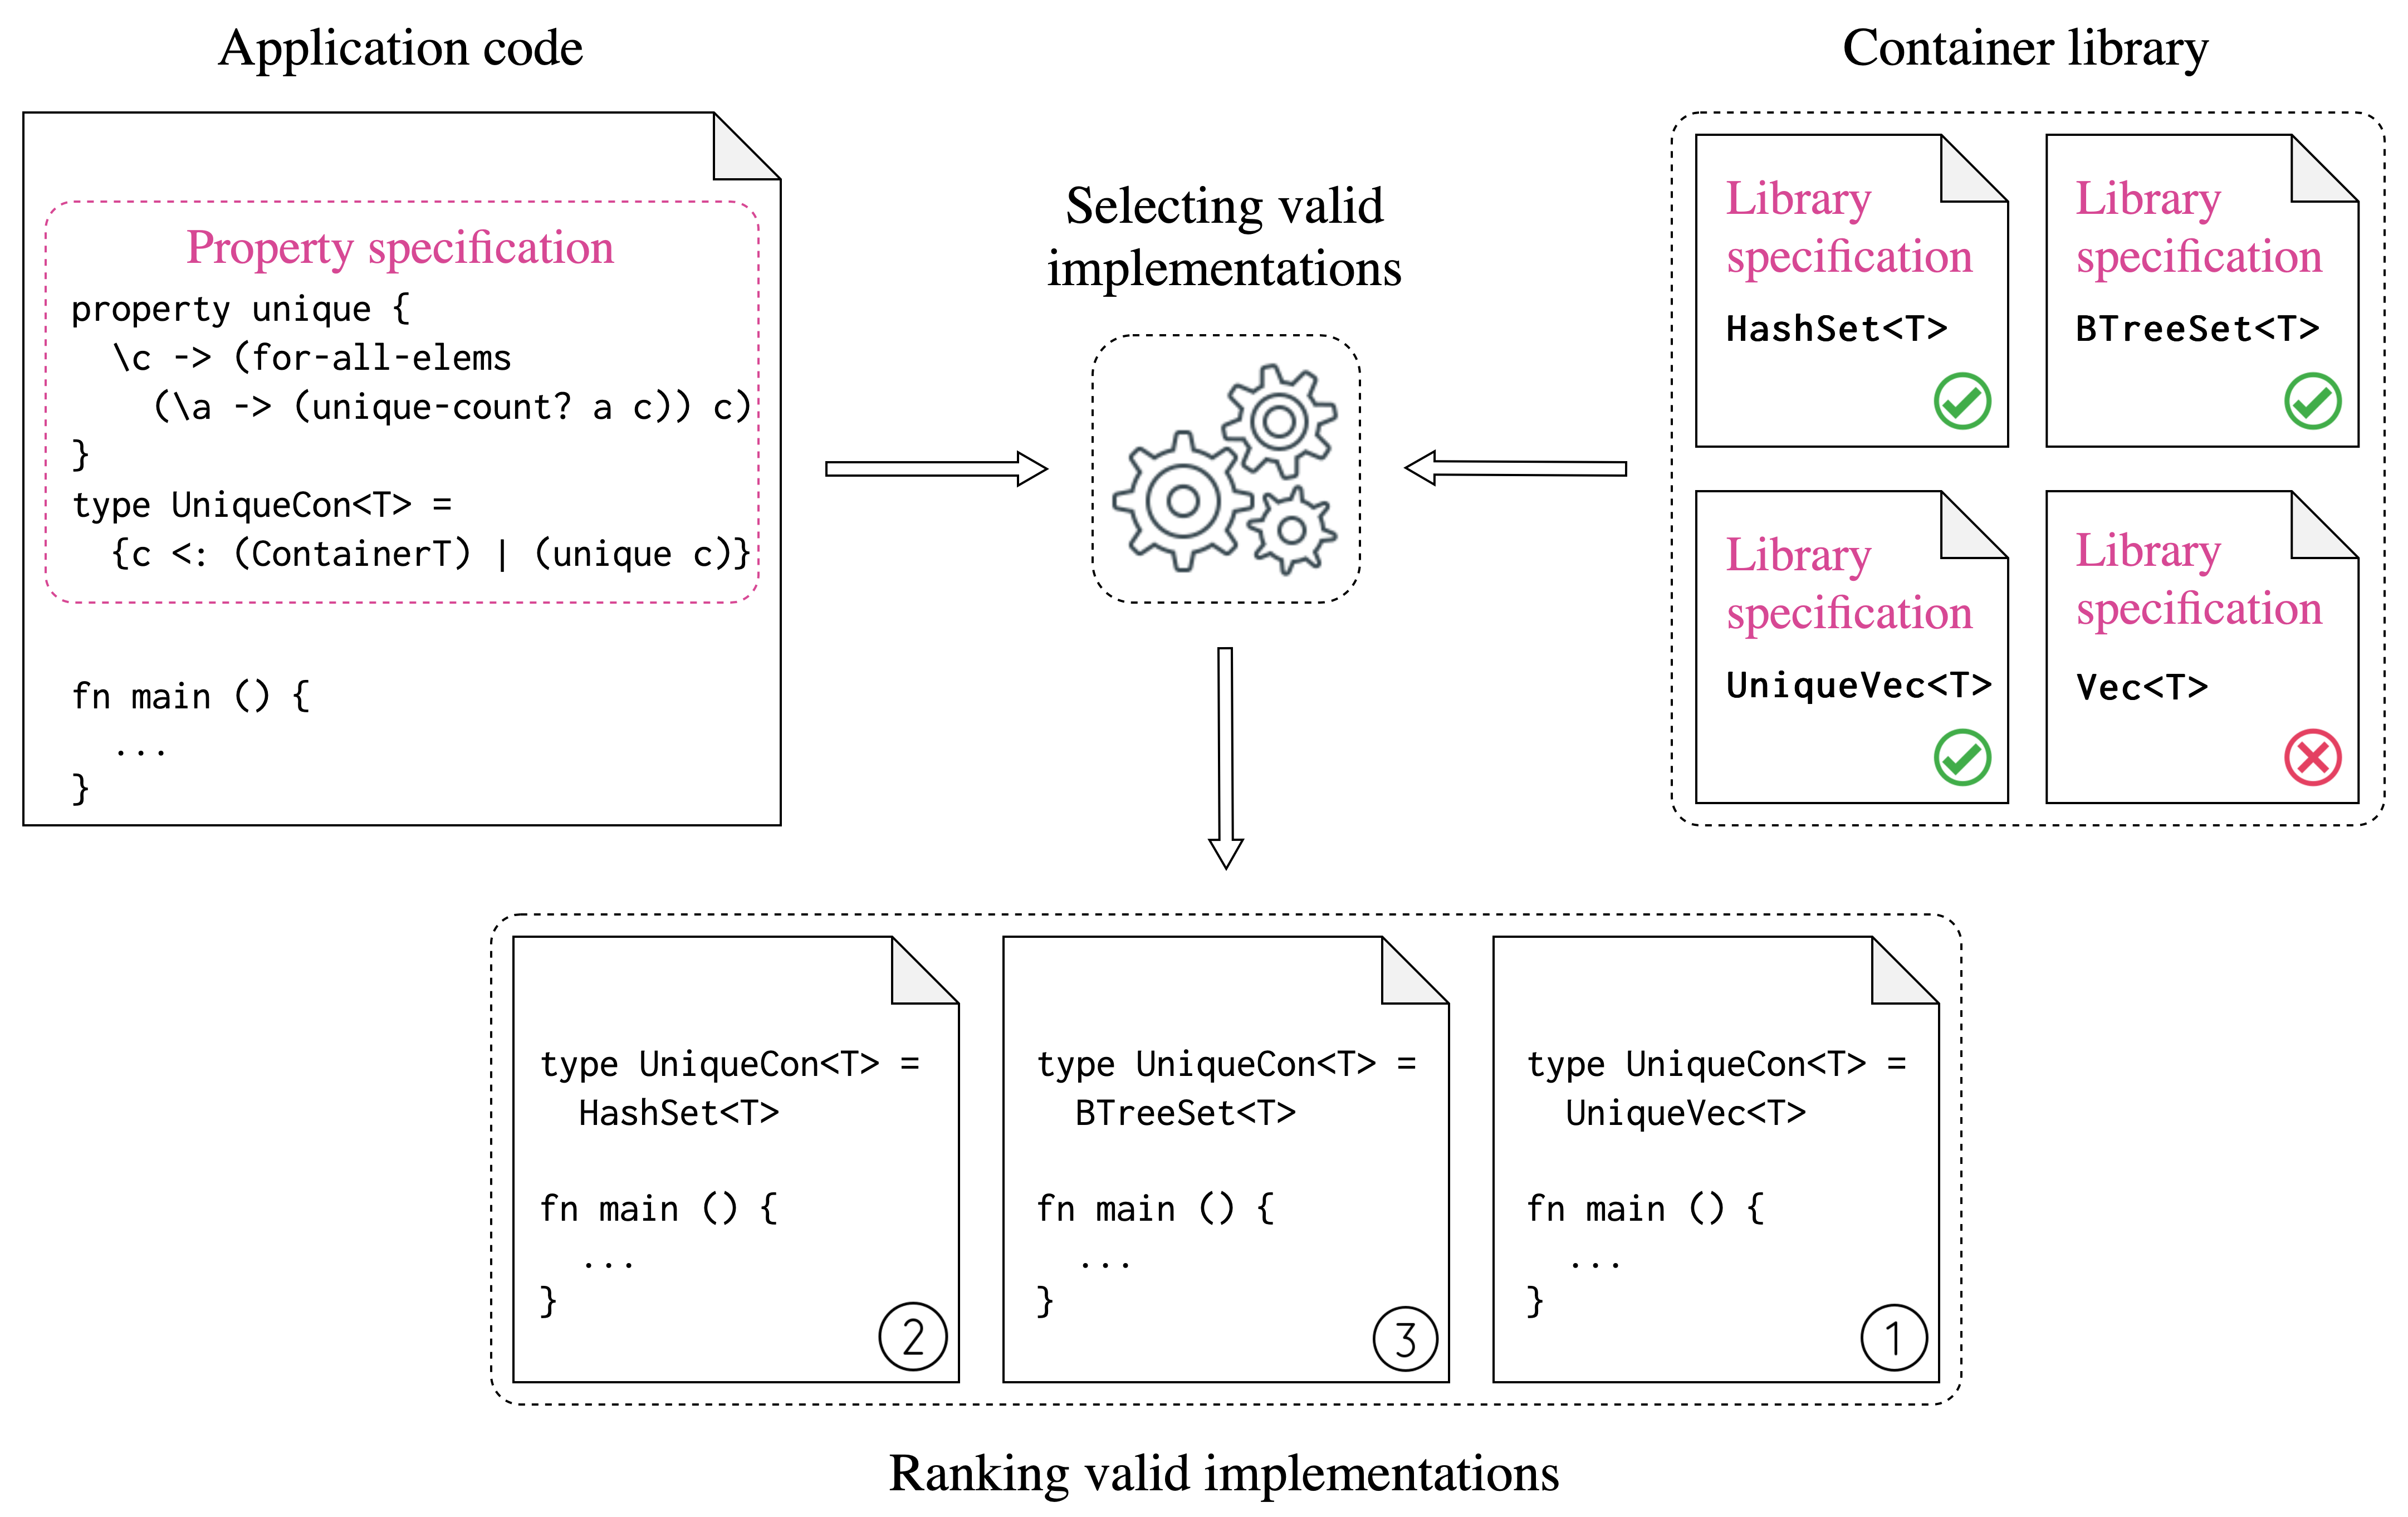
\includegraphics[width=0.95\textwidth]{./overview.png}
    \caption{The workflow of \Primrose{}:
    \emph{Property specifications} (top left), written and used by the application developer, are used to check which \emph{library specifications} (top right), written by library developers, satisfy them.
    Valid implementations (marked with a green check marks), are then ranked by their performance (bottom).
    }
    \label{overview:design}
\end{figure}

Given this code as input, \Primrose{} will, acting as 
a preprocessor, generate copies of the input code where the abstract type is instantiated into a valid concrete implementation that satisfies the expected properties. It determines 
which implementations are valid by consulting \emph{library specifications}, which are provided by library developers. These specifications abstract over concrete container implementations 
and provide a summary of their externally observable semantics. 
For each implementation, the library specification contains the pre- and post-conditions of each operation in terms of an abstract list model. We discuss these specifications in more detail in 
section~\ref{chap2:lib}. 

In our example in 
figure~\ref{overview:design}, the library specification of the \lstinline{Vec<T>} type indicates that it is not a suitable choice for \lstinline{UniqueCon<T>}, as it does not satisfy the required semantic property \lstinline{unique}.
We use a satisfiability modulo theories (SMT) solver for the selection process, which we discuss in section~\ref{chap2:select}.

Figure~\ref{overview:design} shows at the bottom a simplified version of the generated programs.
Note that in order to make \ref{overview:design} concise, we only show a simplified version of the generated programs with selected implementations that does not reflect how traits constrain available operations for interacting with the container type.
In our implementation, we ensure that only the container operations that the application developer specifies with syntactic properties are accessible in the generated program.
%
% After all valid container implementations are selected, \Primrose{} measures and ranks them according to their performance, and then selects the one providing the best performance for the program.
% We discuss the ranking in \ref{chap2:rank}.
%
Our current prototype of \Primrose{} focuses on ensuring the functional correctness of selecting container implementations based on desired properties.
Nevertheless, we have implemented a simple process that ranks valid implementations by their runtime performance.
Rankings by other non-functional metrics could easily be added to our design.
We provide discussion about code generation and ranking in section~\ref{chap2:rank}.

% Porting to other languages
% We discuss the portability of \Primrose{} in \ref{chap2:evaluation}.
% \paragraph{Using Rosette for Designing Specifications and the Selection Process}
\paragraph*{Using Rosette as the Common Language for Specifications and Selection}
\label{common-language}
The ``solver-aided programming language'' Rosette~\citep{rosette-lang, rosette-paper} is used as the common language in \Primrose{} for the formal parts.
Rosette is chosen for \Primrose{} due to its convenient interface to the Z3 SMT solver and the straightforward translation from \Primrose{} property specifications into Rosette.
Property specifications are used as verification conditions when selecting implementations by checking against library specifications which are directly encoded in Rosette. The selection process is done by interacting with the SMT solver via Rosette.


\paragraph*{Portability of \Primrose{}}
\label{implementation:portability}
Currently, we choose Rust as the target language to implement our idea. Application developers write the property specifications as a part of their Rust programs and \Primrose{} generates Rust code after processing specifications. 
However, \Primrose{} could easily be ported to many other languages, since property specifications, 
library specifications, and the process of selecting implementations are all language-agnostic and not attached to Rust's particular type system or language features.
Adapting property specifications into other languages only requires such languages to have a construct similar to Rust's traits, 
such as traits in Scala and interfaces in Java, allowing us to model syntactic properties. It would be straightforward to add new backends to \Primrose{} to 
generate code in these languages. Our library specifications are, by design, an abstraction over implementation details, describing the intended semantics of container operations without respect to 
their implementation. This means we can trivially adapt these specifications to container libraries from other languages, so long as our specifications remain an abstraction of the 
new implementations.  Thus, we anticipate that \Primrose{} could easily be adapted to produce code in any language with sufficient support for data abstraction, such as Java, Scala, Swift, or \Cpp.

\section{Property Specifications}
\label{chap2:prop}
The application developer specifies the desired behaviours of their required container with a \textit{property specification},
% that consists of \emph{semantic properties}, which refine the container type by a predicate, and \emph{syntactic properties}, which in Rust are traits specifying the operations that must be supported by the container and their types.
%
%The property specification of the type \lstinline{UniqueCon} from the example in \ref{overview:design} is:
for example, for the type \lstinline{UniqueCon} from figure~\ref{overview:design}:
\begin{lstlisting}[language=Rust, style=boxed, escapechar=!]
!\tikz[remember picture, overlay]\node [xshift=12.8cm, yshift=+.075cm, inner sep=0.075cm, rectangle] {\footnotesize\bfseries\texttt{Primrose}};!property unique 
  { \c -> (for-all-elems (\a -> (unique-count? a c)) c) }
type UniqueCon<T> = {c <: (ContainerT) | (unique c)}
\end{lstlisting}

We first define the \emph{semantic property} \lstinline{unique} using a \emph{predicate}.
In our specification language, such predicates have type $\mathit{Con}\langle\tau\rangle \to \mathit{Bool}$, where $\mathit{Con}\langle\tau\rangle$ is a placeholder that is resolved into a concrete container type by 
the selection process. The combinator \lstinline{for-all-elems} is part of a library enabling to write predicates for individual container elements. The predicate \lstinline{unique-count?} holds if and only if the given element occurs exactly once in the container. These combinators and predicates are explained in section~\ref{chap2:prop:semantic}.

With the defined \emph{semantic property} \lstinline{unique}, we can then declare the container type \lstinline{UniqueCon<T>}. 
The first part of the declaration specifies the syntactic property that must be satisfied by the container type, in the form of the trait 
\lstinline{ContainerT}. Specifically, \lstinline{c <: (ContainerT)} says that the type of the container \lstinline{c} must implement the trait \lstinline{ContainerT}, which specifies a set of basic container operations. 
The second part of the declaration \emph{refines} our container type by the predicate \lstinline{unique}, stating that the property must be invariant across all container operations.
Properties may also be composed. For multiple syntactic properties, we specify a list of traits (\lstinline{c <: (T1, T2)}) that the container type implements. For multiple semantic properties, we use conjunction, i.e.\ \lstinline{((p1 c) and (p2 c))}.

\begin{figure}[t]
  \begin{alignat*}{3}
  \mathrm{Literals} \quad 
  &l \ &\metaDef \quad &\mathit{true} \cmid \mathit{false}
  \\[-.25em]
  \mathrm{Terms} \quad
  &t \ &\metaDef \quad &l \cmid x \cmid \lambda x.\ t \cmid t\ t
  \\[-.25em]
  %\mathrm{Predicate} \quad 
  %&p \ &\metaDef \quad &\lambda x.\ t
  %\\[-.25em]
  \mathrm{Refinement} \quad 
  &r \ &\metaDef \quad &t \cmid r \wedge r
  \\[-.25em]
  \mathrm{Container\ Type\ Declarations} \quad 
  &c \ &\metaDef \quad &\{v \ \metaBound\ B \mid r\}
  \\[-.25em]
  \mathrm{Simple\ Types} \quad 
  &\sigma \ &\metaDef \quad &\mathit{Bool} \cmid T \cmid \mathit{Con}\langle\sigma\rangle 
  \\[-.25em]
  \mathrm{Types} \quad 
  &\tau \ &\metaDef \quad &\sigma \cmid \tau \to \tau \cmid \forall T \metaBound B .\ \tau
  \\[-.25em]
  \mathrm{Bounds} \quad
  &B \ &\metaDef \quad &\mathit{trait\_name} \cmid B \sep B
  %\\[-.25em]
  %\mathrm{Kinds} \quad 
  %&\kappa \ &\metaDef \quad &\mathsf{type} \cmid \kappa_1 \Rightarrow \kappa_2
  \end{alignat*}
  \caption{The syntax of property specifications. $T$ is the type variable, ranging over element types of the target language, which is Rust in this case.}
  \label{prop:syntax}
\end{figure}

Figure~\ref{prop:syntax} shows the syntax of the \Primrose{} property specification language. Formally, the specification language is a variant of the polymorphic $\lambda$-calculus~\citep{DBLP:conf/programm/Reynolds74, DBLP:journals/tcs/Girard86}, with 
restrictions on the use of polymorphism to enable implicit type inference~\citep{hindley1969principal, MILNER1978348}.
This type system guarantees termination, making specifications easier to analyse and straightforward to translate into SMT verification conditions in Rosette.
The translation into Rosette is straightforward, as terms in the \Primrose{} property specification language (literals, variables, lambdas, and function application) are translated into their counterparts in the functional Rosette language. 

\subsection{Syntactic Properties as Traits}
\label{chap2:prop:syntactic}
In our \Primrose{} prototype, we encode syntactic properties as Rust traits, specifying the operations needed by the application developer to interact with a container. 
Traits are defined in Rust and lifted into our property specification language. For instance, the trait \lstinline|ContainerT| introduced above is implemented as:
\begin{lstlisting}[language=Rust, style=boxed, escapechar=!]
!\tikz[remember picture, overlay]\node [xshift=12.95cm, yshift=+.075cm, inner sep=0.075cm, rectangle] {\footnotesize\bfseries\texttt{Rust}};!pub trait ContainerT<T> {
  fn len(&self) -> usize;
  fn contains(&self, x: &T) -> bool;
  fn is_empty(&self) -> bool;
  fn insert(&mut self, elt: T);
  fn clear(&mut self);
  fn remove(&mut self, elt: T) -> Option<T>;}
\end{lstlisting}

By writing \lstinline{c <: ContainerT}, the application developer indicates that they expect the container type selected by \Primrose{} to include implementations for all operations in the trait \lstinline{ContainerT}. 
Thus, after executing \Primrose{}, \mylstinline{UniqueCon<T>} will be resolved into a concrete container type that implements the trait \lstinline{ContainerT}.

As mentioned, we can also declare a container type that satisfies multiple syntactic properties. For instance, suppose that in addition to \lstinline{ContainerT}, we would like our container to also satisfy the syntactic property \lstinline{IndexableT}:
\begin{lstlisting}[language=Rust, style=boxed, escapechar=!]
!\tikz[remember picture, overlay]\node [xshift=12.95cm, yshift=+.075cm, inner sep=0.075cm, rectangle] {\footnotesize\bfseries\texttt{Rust}};!pub trait IndexableT<T> {
  fn first(&self) -> Option<&T>;
  fn last(&self) -> Option<&T>;
  fn nth(&self, n: usize) -> Option<&T>;
}
\end{lstlisting}

With just \lstinline{ContainerT}, there is no way to observe the \emph{ordering} of elements in the container, but with \lstinline{IndexableT} there is, as we can now select elements based on their position.
By composing our new syntactic property \lstinline{IndexableT} with \lstinline{ContainerT} we can now 
specify a container of unique elements where the order can be observed:
\begin{lstlisting}[language=Rust, style=boxed, escapechar=!]
!\tikz[remember picture, overlay]\node [xshift=12.8cm, yshift=+.075cm, inner sep=0.075cm, rectangle] {\footnotesize\bfseries\texttt{Primrose}};!type UniqueIndexableCon<T> = 
  { c <: (ContainerT, IndexableT) | (unique c) }
\end{lstlisting}

Semantic properties, such as \lstinline{unique}, must be invariant across all operations from all syntactic properties required of the container.
%\todo[author=Michel]{Removed the following snipped, as I think this is redundant}

\subsection{Semantic Properties as Predicates}
\label{chap2:prop:semantic}
As mentioned, semantic properties are predicates that are used to construct refinements for container types; each declared container type in the form $\{v \ \metaBound\ B \mid r\}$ is a \textit{refinement type}, i.e.\ a type circumscribed by a logical predicate~\citep{10.1145/113445.113468}. When the predicates are in SMT-decidable logic, they can be statically checked~\citep{10.1145/1863543.1863560}.
Such techniques are used in programming languages like Liquid Haskell and F*, where they are used to facilitate verification of program correctness. 
For instance, in Liquid Haskell, we may define a refinement type \lstinline{UniqueList} representing a list of unique elements as:
% , caption={Unique List in Liquid Haskell}, captionpos=b, label=prop:lh-uniquelist]
\begin{lstlisting}[language=haskell, style=boxedlst, escapechar=!]
!\tikz[remember picture, overlay]\node [xshift=12.5cm, yshift=+.075cm, inner sep=0.075cm, rectangle] {\footnotesize\bfseries\texttt{Liquid Haskell}};!{-@ measure unique @-}
unique :: (Ord a) => [a] -> Bool
unique [] = True
unique (x:xs) = unique xs && not (S.member x (elts xs))
{-@ type UniqueList a = {v:[a] | unique v} @-}
\end{lstlisting}

\noindent While our syntax for type refinements strongly resembles Liquid Haskell, our refinement types are slightly different, and serve a different purpose.
Firstly, Liquid Haskell's refinements 
are attached to a \emph{concrete type}, in this case a list (written \lstinline{[a]}), whereas our refinements are attached to an abstract container type, which is then resolved by \Primrose{} into a concrete 
implementation. Secondly, Liquid Haskell 
uses type refinements for the purpose of \emph{correctness}: If a list is declared to have type \lstinline{UniqueList}, the Liquid Haskell verifier will check that it satisfies the predicate \lstinline{unique}. 
The \lstinline{notUniqueList} shows that it will report an error at compile time if a given list contains duplicates.
\begin{lstlisting}[language=haskell, style=boxedlst, escapechar=!]
!\tikz[remember picture, overlay]\node [xshift=12.5cm, yshift=+.075cm, inner sep=0.075cm, rectangle] {\footnotesize\bfseries\texttt{Liquid Haskell}};!{-@ notUniqueList :: UniqueList Int @-}
notUniqueList::[Int]
notUniqueList = [3, 1, 2, 3]
\end{lstlisting}
Our work instead uses type refinements to specify the semantic requirements of the application developer to guide selection of valid concrete implementations.
Once all valid implementations have been found, \Primrose{} simply selects the implementation providing the best performance for the application developer.
In short, rather than to aid verification, we use refinement types to help application developers optimise their programs. We give more details on the selection process in section~\ref{chap2:select}.

\paragraph*{Combinators and Predicate Functions} Demonstrated by our examples, \Primrose{} provides a set of combinators and predicate functions to facilitate writing of property specifications. 
These combinators and predicate functions are defined in Rosette and then imported into our property 
specification language.  In the semantic property \lstinline{unique}, the combinator \lstinline{for-all-elems} is used to specify that the predicate \lstinline{unique-count?} must hold for all elements inside the container. 
The type of the combinator \lstinline{for-all-elems} is $\mathit{Con}\langle\tau\rangle \to (\tau \to \mathit{Bool}) \to \mathit{Bool}$, meaning this combinator takes in two arguments, the first of which is a container and the second of which is a predicate on the elements of that container, and eventually returns a boolean value.

For the purposes of checking, we represent containers $\mathit{Con}\langle\tau\rangle$ abstractly in Rosette as lists. We discuss this list abstraction and justify it in section~\ref{chap2:lib}.
With such a list abstraction, we are able to straightforwardly implement our \lstinline{for-all-elems} combinator with a list fold operation:
\begin{lstlisting}[language=racket, style=boxed, label=prop:combinator-unary, escapechar=!] 
!\tikz[remember picture, overlay]\node [xshift=12.8cm, yshift=+.075cm, inner sep=0.075cm, rectangle] {\footnotesize\bfseries\texttt{Rosette}};!(define (for-all-elems c fn)
    (foldl elem-and #t (map (lambda (a) (fn a)) c)))
\end{lstlisting}

We also provide some combinators for applying \emph{relations} between elements in a container. For instance, the combinator \mylstinline{for-all-consecutive-pairs}:
\begin{align}
    \label{prop:combinator-pair}
    \texttt{for-all-consecutive-pairs}\; :\; \mathit{Con}\langle\tau\rangle \to (\tau \to \tau \to \mathit{Bool}) \to \mathit{Bool}
\end{align}
Unlike \lstinline{for-all-elems}, this combinator gives a binary relation between elements, and checks that this relation holds between any two consecutive elements in a container.

With the combinator \lstinline{for-all-consecutive-pairs} and the predicates \lstinline{geq?} and \lstinline{leq?}, we can define properties like \lstinline{ascending} and \lstinline{descending}, which specify particular orderings of elements in a container:
\begin{lstlisting}[language=Rust, style=boxed, escapechar=!]
!\tikz[remember picture, overlay]\node [xshift=12.8cm, yshift=+.075cm, inner sep=0.075cm, rectangle] {\footnotesize\bfseries\texttt{Primrose}};!property ascending { \c -> (for-all-consecutive-pairs c leq?) }
property descending { \c -> (for-all-consecutive-pairs c geq?) }
\end{lstlisting}

Besides the set of combinators and predicate functions predefined in \Primrose{}, application developers may also provide customised functions by providing Rosette definitions and importing them into our property specification language. 

\paragraph*{Composition of semantic properties} As shown in figure~\ref{prop:syntax}, we can compose semantic properties in a container type declaration with conjunction.
For instance, to declare a container type with elements arranged in \emph{strictly} ascending order, i.e., both \lstinline{unique} and \lstinline{ascending} properties must hold, we can write the following:
\begin{lstlisting}[language=Rust, style=boxed]
!\tikz[remember picture, overlay]\node [xshift=12.8cm, yshift=+.075cm, inner sep=0.075cm, rectangle] {\footnotesize\bfseries\texttt{Primrose}};!type StrictlyAscendingCon<T> = 
  { c <: (ContainerT) | ((unique c) and (ascending c)) }
\end{lstlisting}
The conjunction \lstinline|and| is directly translated into a conjunction operation in Rosette.

\subsection{The Interaction between Semantic Properties and Syntactic Properties}
\label{chap2:prop:semantic-syntactic}
All semantic properties we have seen so far have been invariants across all operations, but 
some semantic properties relate to specific operations given by syntactic properties. 
For instance, when specifying a stack container type providing operations \lstinline{push} and \lstinline{pop} with the expected last-in-first-out (LIFO) property.
% on top of the trait \lstinline{ContainerT} specifying basic container operations, 
Firstly, we define a trait specifying operations \lstinline{push} and \lstinline{pop}, namely \lstinline{StackT}:
\begin{lstlisting}[language=Rust, style=boxed, caption=The trait \mylstinline{StackT} specifying operations \mylstinline{push} and \mylstinline{pop}, captionpos=t, label=prop:spec-stackt, escapechar=!]
!\tikz[remember picture, overlay]\node [xshift=12.95cm, yshift=+.075cm, inner sep=0.075cm, rectangle] {\footnotesize\bfseries\texttt{Rust}};!pub trait StackT<T> {
  fn push(&mut self, elt: T);
  fn pop(&mut self) -> Option<T>;
}
\end{lstlisting}
Secondly, we define the semantic property \lstinline{lifo} for containers that implement \lstinline{StackT}:
\begin{lstlisting}[language=Rust, style=boxed, caption=The semantic property LIFO, captionpos=t, label=prop:spec-lifo, escapechar=!]
!\tikz[remember picture, overlay]\node [xshift=12.8cm, yshift=+.075cm, inner sep=0.075cm, rectangle] {\footnotesize\bfseries\texttt{Primrose}};!property lifo { \c <: StackT -> (forall \x. pop (push c x) == x) }
\end{lstlisting}
\noindent
Unlike previously, this semantic property includes a requirement that the given container implements the trait \lstinline{StackT}, enabling us to refer to the operations \lstinline{pop} and \lstinline{push} inside the semantic property. In this definition, \lstinline{forall} is a combinator with type:
\begin{align}
    \label{prop:combinator-forall}
    \texttt{forall}\; :\; \forall x. \,(x \to \mathit{Bool}) \to \mathit{Bool}
\end{align}
This combinator is implemented with the \lstinline{forall} procedure defined in Rosette's library, which serves as a construct for creating universally quantified formulae.

Armed with the trait \lstinline{StackT} and the semantic property \lstinline|lifo|, we can combine all these elements and declare our stack type as follows:
%  caption=The container type with stack operations satisfying the semantic property LIFO, captionpos=b,
\begin{lstlisting}[language=Rust, style=boxed, escapechar=!]
!\tikz[remember picture, overlay]\node [xshift=12.8cm, yshift=+.075cm, inner sep=0.075cm, rectangle] {\footnotesize\bfseries\texttt{Primrose}};!type StackCon<T> = {c <: (ContainerT, StackT) | (lifo c)}
\end{lstlisting}

In the next section, we will discuss how library developers write specifications for their container implementations.

%\Primrose{} selects among these library specifications the ones that satisfy the properties required by application developers.

\section{Library Specifications}
\label{chap2:lib}
% show full spec
% unique + lifo
% verification
% no good rust semantic framework for verification yet; rust belt in dev.
%
% TODO: Should we remove this to streamline the presentation (this feels a bit like a re-motivation of the points we made already in the introduction)
% It is not feasible to select container implementations directly by analysing their Rust source code and checking if they satisfy the properties specified by the application developer.
% Rust is a Turing-complete, general purpose programming language with a complex semantics, and its container libraries 
% are typically highly optimised, making extensive use of unsafe code. Doing such a broad analysis precisely and automatically is very hard even for the most advanced of static analyses.
% Instead, we write 
\emph{Library specifications} abstract over Rust container implementations, providing a clear definition of intended semantics of each operation, without respect to performance or implementation details. 
This approach allows us to select container implementations by simply checking their library specifications, rather than their full implementations, against the properties specified by the application developer.
Moreover, using specifications which are abstracted from implementations makes \Primrose{} easy to repurpose for programming languages other than Rust, as the same specifications would apply, with minimal or no modification, to container libraries written in any other language. 

By encoding these specifications into \emph{property based tests}, which validate container implementations against their library specifications (section~\ref{chap2:evaluation:testing}), we ensure the selected implementations indeed satisfy a required property specification. Since these library specifications form a \emph{functional correctness} specification for each operation, they could also be used in future as the basis of full functional correctness verification with a verification framework for Rust~\citep{rustbelt-paper}, but this is out of scope for \Primrose{}.

\subsection{The Basic Design of Library Specifications}
\label{chap2:lib:design}
Library specifications of concrete container implementations are developed based on Hoare logic~\citep{10.1145/363235.363259}.
For each concrete container implementation, we provide a set of \emph{Hoare triples}, one for each operation. A Hoare triple of the form
$\{\phi\}\; \mathsf{op} \;\{\psi\}$ states that if the \textit{precondition} $\phi$ holds and the operation $\mathsf{op}$ is executed, then the \textit{postcondition} $\psi$ will hold.
These conditions are predicates on the state of the program. In our case, the state contains the container, plus any other inputs and outputs of the operation $\mathsf{op}$.

As mentioned in section~\ref{chap2:overview}, we model the container as a list in Rosette for \Primrose{}'s library specifications. The list is a model to convey the intended semantics, and does not proscribe anything about the implementation --- the implementation is free to represent 
data in any chosen structure. For example, a set data type may be implemented with a binary search tree, but will still be specified with a list. 
These model lists are a simple abstraction, easy to analyse, with which all container operations can be specified.

\paragraph*{Library Specifications Convey the Intended Semantics for Implementations} It is important that all possible executions of a concrete implementation should be captured by its library specification. Otherwise in the process of selecting implementations by checking if their library specifications match the required semantic property, \Primrose{} could select an unsatisfying implementation. More formally, a proof of functional correctness of an implementation w.r.t. its specification would take the form of a data refinement~\citep{de_roever_engelhardt_1998},
where each value of the concrete container type is related to our list model by an \emph{abstraction function} $\alpha$, and our specification on lists is shown to contain all possible behaviours 
of the concrete implementation using a \emph{forward simulation}:
% \begin{figure}[!ht]
\vspace{-.5em}
\begin{center}
  $\begin{array}{c}\alpha^{-1};\mathsf{op(\textit{C})}  \subseteq
  \mathsf{op(\textit{A})}; \alpha^{-1}\quad\\\text{\footnotesize (where ; is forward composition of relations} \\\text{\footnotesize and $\alpha^{-1}$ is the inverse relation of $\alpha$)}\end{array}$
\begin{tikzcd}[row sep=1.2cm,column sep=1.2cm,inner sep=0.7ex, cramped]
\circ
\arrow[Mapsto]{r}[name=U]{\textsf{op(\textit{A})}}
\arrow[dr, rounded corners,
       to path={ ([xshift=1.3ex,yshift=-0.5ex]\tikztostart.south) |- ([yshift=1.3ex,xshift=-0.5ex]\tikztotarget.west)}]
\arrow[dr, rounded corners,
       to path={ ([yshift=-1.3ex,xshift=0.5ex]\tikztostart.east) -| ([xshift=-1.3ex, yshift=0.5ex]\tikztotarget.north)}]
&
\circ
\\
\bullet
\arrow[dashed]{u}{\alpha}
\arrow[swap, Mapsto]{r}[name=D]{\textsf{op(\textit{C})}}
&
\bullet
\arrow[swap,dashed]{u}{\alpha}
\arrow[to path={(U) node[midway,scale=1.5] {\rotatebox[origin=c]{90}{$\subseteq$}}  (D)}]{}
\end{tikzcd}
\end{center}
% \caption{Forward simulation} \label{lib:forward-simulation}
% \end{figure}

\noindent Here, $\mathsf{op(\textit{C})}$ denotes the concrete implementation of our operation $\mathsf{op}$, represented as a relation from inputs to outputs.
The abstract operation $\mathsf{op(\textit{A})}$ is the maximal relation satisfying the Hoare triple given in our library specification, and $\alpha$ is a suitable abstraction function that 
flattens a concrete container into a list. 

If a forward simulation is shown for all operations, we can then conclude that each possible execution with the concrete container implementation has a corresponding execution with an abstract list, thus the specification accurately captures the implementation's semantics.

For instance, a binary search tree $T$ can be abstracted to a sorted list $L$ by an abstraction function $\mathit{inorder}$ that does an in-order traversal. For each operation interacting with $T$, there exists a corresponding operation at the abstract level defined using $L$. 
Take the operation $\mathsf{insert(\textit{T},x)}$, which inserts an element $x$ into a binary search tree $T$. We can abstract such an operation to $\mathsf{insert(\textit{L},x)}$ which inserts $x$ at the right location in a sorted list. The relation between these two operations is shown by this diagram:
\vspace{-.4em}
\begin{center}
 % $\begin{array}{c}\mathit{inorder}(\mathsf{insert}(\textit{T},x)) \mathit{inorder}^{-1};\mathsf{len(\textit{T})}  \subseteq
 % \mathsf{len(\textit{L})}; inorder^{-1}\quad\end{array}$
\begin{tikzcd}[row sep=1.2cm,column sep=1.2cm,inner sep=0.7ex, cramped]
\circ
\arrow[Mapsto]{r}[name=U]{\textsf{insert(\textit{L},x)}}
\arrow[dr, rounded corners,
       to path={ ([xshift=1.3ex,yshift=-0.5ex]\tikztostart.south) |- ([yshift=1.3ex,xshift=-0.5ex]\tikztotarget.west)}]
\arrow[dr, rounded corners,
       to path={ ([yshift=-1.3ex,xshift=0.5ex]\tikztostart.east) -| ([xshift=-1.3ex, yshift=0.5ex]\tikztotarget.north)}]
&
\circ
\\
\bullet
\arrow[dashed]{u}{\mathit{inorder}}
\arrow[swap, Mapsto]{r}[name=D]{\textsf{insert(\textit{T},x)}}
&
\bullet
\arrow[swap,dashed]{u}{\mathit{inorder}}
\arrow[to path={(U) node[midway,scale=1.5] {\rotatebox[origin=c]{90}{$\subseteq$}}  (D)}]{}
\end{tikzcd}
\end{center}
\vspace{-.4em}
\noindent In this work, we specified four container implementations from Rust's standard library (\lstinline!Vec!,\,\lstinline!LinkedList!,\,\lstinline!HashSet!,\,\lstinline!BTreeSet!) and four custom container implementations (\lstinline!SortedVec!,\,\lstinline!LazySortedVec!,\,\lstinline!UniqueVec!,\,\lstinline!LazyUniqueVec!) by abstracting them into a list model.
As we discuss in section~\ref{chap2:lib:abstracting}, library specifications abstract over some implementation details, and, thus, \lstinline!Vec! and \lstinline!LinkedList! share the same specifications, as do the eager and lazy \lstinline!SortedVec! and \lstinline!UniqueVec! implementations.
For each specification, we define a suitable abstraction function for forward simulation which, while not needed for selection, is used for property-based testing to justify that a concrete implementation satisfies the intended semantics described by its library specification.

\paragraph*{Completeness of Library Specifications} 
While it is important to ensure that library specifications indeed convey the intended semantics of the implementation, \emph{completeness} of library specifications is also important. Without completeness, \Primrose{} could possibly rule out perfectly valid implementations because it cannot prove that the required semantic properties are preserved for an operation of which the specification is incomplete. 

Our approach easily ensures completeness when each operation is specified by a \emph{deterministic} model operation. Forward simulation states that every execution of the concrete implementation has a corresponding execution in the abstract operation, while determinism states that such correspondence is one-to-one, i.e., each abstract execution also has a corresponding concrete one.
Thus, just as forward simulation states that each property established for an abstract operation applies also (via the inverse of the abstraction function $\alpha^{-1}$) to a concrete implementation, completeness states that each property established for a concrete implementation applies (via the abstraction function $\alpha$) to the abstract operation. With both completeness and forward simulation, we ensure that \emph{all} valid implementations and \emph{only} the valid implementations are selected by \Primrose{}.

There are many other availiable approaches for modelling library specifications, for instance, the axiomatic approach used in algebraic specifications for abstract data types \cite{WIRSING1990675}, specifying the behaviour of operations as a set of equational axioms that relate various operations.
However, it is hard to ensure the completeness of algebraic specifications, as it is hard capture all behaviours of all operations by a set of equations.  

\subsection{The Library Specification of A \texttt{LinkedList}}
\label{chap2:lib:list}
Rust's \lstinline{LinkedList} is a doubly-linked list. The abstraction function to convert it into a logic list is straightforward: Collect all nodes' values with previous and next pointers.

Firstly, we specify the insertion operation, \lstinline|LinkedList::insert|, of which the type signature is:
% caption=The signature of \mylstinline{LinkedList::insert}, captionpos=b, label=lib:sig-list-insert
\begin{lstlisting}[language=Rust, style=boxed, escapechar=!]
!\tikz[remember picture, overlay]\node [xshift=12.95cm, yshift=+.075cm, inner sep=0.075cm, rectangle] {\footnotesize\bfseries\texttt{Rust}};!fn insert(&mut self, elt: T) {...}
\end{lstlisting}
\noindent
Since variables in Rosette are immutable, in the corresponding abstract insertion operation, we alter the type to return a new list instead of altering the list in-place\footnote{Rosette is untyped, but this is morally the type signature.}:
%, caption=The signature of the abstract operation corresponding to \mylstinline{LinkedList::insert}, captionpos=b, label=lib:sig-abs-insert
\begin{lstlisting}[language=racket, style=boxed]
!\tikz[remember picture, overlay]\node [xshift=12.8cm, yshift=+.075cm, inner sep=0.075cm, rectangle] {\footnotesize\bfseries\texttt{Rosette}};!abs-insert: List<T> -> T -> List<T>
\end{lstlisting}
We can then provide the specification of \lstinline|LinkedList::insert| with respect to its corresponding abstract operation, the maximal relation satisfying the Hoare triple:
\begin{align}
\label{lib:spec-list-insert}
\{xs_0.\ \texttt{\small true}\}~\texttt{abs-insert}~\{xs_0\ x\ xs.\ xs = \texttt{\small model-insert}\ xs_0\ x\}
\end{align}
Here, $xs_0$ refers to the initial value of the container, $xs$ refers to the resultant container, and $x$ is the element we insert. The function \lstinline|model-insert| is defined in Rosette on lists:
%, caption=The model insertion operation, captionpos=b, label=lib:logic-list-insert
\begin{lstlisting}[language=racket, style=boxed]
!\tikz[remember picture, overlay]\node [xshift=12.8cm, yshift=+.075cm, inner sep=0.075cm, rectangle] {\footnotesize\bfseries\texttt{Rosette}};!(define (model-insert xs x) (append xs (list x)))
\end{lstlisting}
The postcondition states that we expect applying the insertion operation to a container to produce the same result as the result produced by \lstinline|model-insert| function. In library specifications, defining such \emph{model operations} is a common technique to simplify writing postconditions. 

Similarly, we also provide the specification for the operation \lstinline{LinkedList::contains}:
%, caption=The signature of \mylstinline{LinkedList::contains}, captionpos=b, label=lib:sig-list-contains
\begin{lstlisting}[language=Rust, style=boxed, escapechar=!]
!\tikz[remember picture, overlay]\node [xshift=12.95cm, yshift=+.075cm, inner sep=0.075cm, rectangle] {\footnotesize\bfseries\texttt{Rust}};!fn contains(&self, x: &T) -> bool {...}
\end{lstlisting}
\noindent
In our corresponding abstract operation, in addition to the boolean value indicating whether the given element \lstinline|x| is present or not, the input container is also returned, as we would like to express the input container is not mutable, its value remains unchanged after this operation. Also, since the underlying value with type \lstinline|T| is given by an immutable reference \lstinline|&T|, in the abstract operation we treat the immutable reference \lstinline|&T| as simply \lstinline|T|. The signature of the abstract operation is shown below:
\begin{lstlisting}[language=racket, style=boxed, caption=The signature of the abstract operation corresponding to \mylstinline{LinkedList::contains}, captionpos=t, label=lib:sig-abs-contains]
!\tikz[remember picture, overlay]\node [xshift=12.8cm, yshift=+.075cm, inner sep=0.075cm, rectangle] {\footnotesize\bfseries\texttt{Rosette}};!abs-contains: List<T> -> T -> (List<T>, bool)
\end{lstlisting}
The Hoare triple that serves as the specification of \lstinline|LinkedList::contains| is:
\begin{align}
\label{lib:spec-list-contains}
\{xs_0.\ \texttt{\small true}\}\ \texttt{abs-contains}\ \{xs_0\ x\ xs\ r.\ (xs, r) = \texttt{\small model-contains}\ xs_0\ x\}
\end{align}
Note that in this specification, the model operation \lstinline|model-contains| defined in listing~\ref{lib:logic-list-contains} has the same type signature as the abstract operation shown in listing~\ref{lib:sig-abs-contains}. It also returns a pair of values: the output list, which is always equal to the input list, and a boolean value indicating if the element is present in the list.
\begin{lstlisting}[language=racket, style=boxed, caption=The model operation for checking an element's containment, captionpos=t, label=lib:logic-list-contains]
!\tikz[remember picture, overlay]\node [xshift=12.8cm, yshift=+.075cm, inner sep=0.075cm, rectangle] {\footnotesize\bfseries\texttt{Rosette}};!(define (model-contains xs x)
  (cond [(list? (member x xs)) (cons xs #t)]
        [else (cons xs #f)]))
\end{lstlisting}
Because \lstinline|model-contains| returns the unchanged list, it specifies that the operation \lstinline|LinkedList::contains| should not change the list. 

The library specification of the list removal operation is slightly more complicated, we use \lstinline|T?| to denote that a type may be \lstinline|null| to express Rust's \lstinline{Option<T>} type, which is the return type of \lstinline|LinkedList::remove|. 
The type signature of \lstinline|LinkedList::remove| is shown below:
%, caption=The type signature of \mylstinline{LinkedList::remove}, captionpos=b, label=lib:sig-list-remove
\begin{lstlisting}[language=Rust, style=boxed, escapechar=!]
!\tikz[remember picture, overlay]\node [xshift=12.95cm, yshift=+.075cm, inner sep=0.075cm, rectangle] {\footnotesize\bfseries\texttt{Rust}};!fn remove(&mut self, x: T) -> Option<T> {...}
\end{lstlisting}
\noindent
This operation removes the first occurrence of an element from the given linked list and returns it. If the linked list does not contain the element, \lstinline|None| is returned and the list remains unchanged.
The signature of the corresponding abstract operation is:
%, caption=The signature of the abstract operation corresponding to \mylstinline{LinkedList::remove}, captionpos=b, label=lib:sig-abs-remove
\begin{lstlisting}[language=racket, style=boxed]
!\tikz[remember picture, overlay]\node [xshift=12.8cm, yshift=+.075cm, inner sep=0.075cm, rectangle] {\footnotesize\bfseries\texttt{Rosette}};!abs-remove: List<T> -> T -> (List<T>, T?)
\end{lstlisting}
The model removal operation has the same signature as the abstract operation. We return \lstinline|null| in Rosette for the \lstinline|None| case:
%, caption=The model removal operation, captionpos=b, label=lib:logic-list-remove
\begin{lstlisting}[language=racket, style=boxed]
!\tikz[remember picture, overlay]\node [xshift=12.8cm, yshift=+.075cm, inner sep=0.075cm, rectangle] {\footnotesize\bfseries\texttt{Rosette}};!(define (model-remove xs x) 
  (cond [(list? (member x xs)) (cons (remove x xs) x)]
        [else (cons xs null)]))
\end{lstlisting}
Again, we return a pair of the resulting list and the element being removed. Then we provide the library specification of \lstinline|LinkedList::remove|:
\begin{align}
\label{lib:spec-list-remove}
\{xs_0.\ \texttt{\small true}\}\ \texttt{abs-remove}\ \{xs_0\ x\ xs\ r.\ (xs, r) = \texttt{\small model-remove}\ xs_0\ x\}
\end{align}
To provide a complete specification of \lstinline|LinkedList|, the library developer must ensure that each operation of the \lstinline|LinkedList| is specified by a trait, and for each operation in each trait the \lstinline|LinkedList| implements, specifications similar to the above are provided.

\subsection{The Library Specification of A \texttt{BTreeSet}}
\label{chap2:lib:btree}
For the \lstinline|LinkedList| it is intuitive to use a logic list as a model, as they are both lists. However, even for non-linear structures such as trees, we can still use logic lists as a model. 
Rust's \lstinline|BTreeSet| is a set implemented using a b-tree.
All elements are unique and arranged in ascending order. Thus, our list model of the b-tree is simply a sorted list in ascending order, where uniqueness of elements is preserved.
The abstraction function $\alpha$ that converts the \lstinline|BTreeSet| to our list model is simply an in-order traversal.

The first example to be illustrated is again the specification of the insertion operation with signature:
%, caption=The signature of \mylstinline{BTreeSet::insert}, captionpos=b, label=lib:sig-tree-insert
\begin{lstlisting}[language=Rust, style=boxed, escapechar=!]
!\tikz[remember picture, overlay]\node [xshift=12.95cm, yshift=+.075cm, inner sep=0.075cm, rectangle] {\footnotesize\bfseries\texttt{Rust}};!pub fn insert(&mut self, value: T) {...}
\end{lstlisting}
\noindent
The signature of the abstract insert operation on our model lists is the same as for \lstinline{LinkedList::insert}.
% resembles the abstraction of \lstinline{LinkedList::insert}:
%, caption=The signature of the abstract operation corresponding to \mylstinline{BTreeSet::insert}, captionpos=b, label=lib:sig-abs-insert-tree
% \begin{lstlisting}[language=racket, style=boxed]
% abs-insert: List<T> -> T -> List<T>
% \end{lstlisting}
The specification of \lstinline{abs-insert} for \lstinline|BTreeSet|, however, differs from that of \lstinline|LinkedList|, as we must maintain ordering and uniqueness of elements:
\begin{align}
\label{lib:spec-tree-insert}
\{xs_0.\ xs_0 = \texttt{\small dedup}\ (\texttt{\small sort}\ xs_0\ \texttt{\small<})\}~\texttt{abs-insert}~\{xs_0\ x\ xs.\ xs = \texttt{\small model-insert}\ xs_0\ x\}
\end{align}
As before, $x$ is the element to be inserted, and $xs_0$ and $xs$ are lists modelling the container (via the in-order traversal function $\alpha$) before and after the \lstinline|abs-insert| operation respectively. 
We place an assertion $xs_0 = \texttt{\small dedup}\ (\texttt{\small sort}\ xs_0\ \texttt{\small<})$ in the precondition requiring that the model $xs_0$ to be a sorted list of unique elements. 
While this precondition should always be satisfied by an in-order traversal of a valid b-tree, we do not want our abstraction to constrain the implementation's behaviour if the data invariants of the b-tree are violated --- given a malformed b-tree, the 
implementation should be free to return any result. Because the semantics of \lstinline{abs-insert} are the maximal relation satisfying this specification, this abstract operation contains all possible behaviours of the concrete implementation if this precondition is violated. The \lstinline|model-insert| here is simply an insertion operation defined on a sorted list of unique elements:
%, caption=The unique and sorted list's model insertion operation, captionpos=b, label=lib:unique-sorted-list-insert
\begin{lstlisting}[language=racket, style=boxed]
!\tikz[remember picture, overlay]\node [xshift=12.8cm, yshift=+.075cm, inner sep=0.075cm, rectangle] {\footnotesize\bfseries\texttt{Rosette}};!(define (model-insert xs x) (dedup (sort (append xs (list x)) <)))
\end{lstlisting}
% \todo[author=XY]{I guess we don't need to talk about the efficiency here?} (Michel: Agree)
% Note that because our specifications do not need to be efficient, we can na\"ively implement this function simply by appending the new element to the list, then sorting and removing duplicates from it.

We can also provide specifications for abstract operations that observe the ordering of elements in a \lstinline|BTreeSet|, such as those operations from the \lstinline|IndexableT| trait, since there is a one-to-one correspondence between each element's position in a \lstinline|BTreeSet| and its position in the model list abstracted from the \lstinline|BTreeSet|.
For instance, we provide the specification of the operation \lstinline|BTreeSet::first|, which is the operation obtaining the first (and also the minimal) element of a \lstinline|BTreeSet| with signature:
%, caption=The signature of \mylstinline{BTreeSet::first}, captionpos=b, label=lib:sig-tree-first
\begin{lstlisting}[language=Rust, style=boxed, escapechar=!]
!\tikz[remember picture, overlay]\node [xshift=12.95cm, yshift=+.075cm, inner sep=0.075cm, rectangle] {\footnotesize\bfseries\texttt{Rust}};!fn first(&self) -> Option<&T> {...}
\end{lstlisting}
\noindent
We again provide the signature of its corresponding abstract operation:
%, caption=The signature of the abstract operation corresponding to \mylstinline{BTreeSet::first}, captionpos=b, label=lib:sig-abs-first-tree
\begin{lstlisting}[language=racket, style=boxed]
abs-first: List<T> -> (List<T>, T?)
\end{lstlisting}
Like \lstinline|LinkedList::contains| in listing~\ref{lib:sig-abs-contains}, this type includes a returned list, as \Primrose{} does not consider the immutability of \lstinline|&self| in the Rust type signature above. 
We again include the requirement that the container is unchanged in the specification:
\begin{align}
\label{lib:spec-tree-first}
\{xs_0.\ xs_0 = \texttt{\small dedup}\ (\texttt{\small sort}\ xs_0\ \texttt{\small<})\}~\texttt{abs-first}~\{xs_0\ xs\ x.\ (xs, x) = \texttt{\small model-first}\ xs_0\}
\end{align}
Here, \lstinline|model-first| is defined as a function that returns the first element of the list, is present, along with the list itself:
%, caption=The model operation obtaining the first element of a list, captionpos=b, label=lib:unique-sorted-list-first
\begin{lstlisting}[language=racket, style=boxed]
!\tikz[remember picture, overlay]\node [xshift=12.8cm, yshift=+.075cm, inner sep=0.075cm, rectangle] {\footnotesize\bfseries\texttt{Rosette}};!(define (model-first xs) 
  (cond 
    [(null? xs) (cons xs null)] 
    [else (cons xs (first xs))]))
\end{lstlisting}
% (define (model-first xs)
%   (cond
%     [(null? xs) (cons xs null)]
%     [else (cons xs (first xs))]))
As before, our precondition includes the assumption that the model $xs_0$ abstracted from the \lstinline{BTreeSet} contains unique elements that are sorted in ascending order. 

\subsection{The Library Specification of A \texttt{HashSet}}
\label{lib:hashset}
A tree implementation of a set maintains its elements in a fixed ascending order, and the ordering of our abstract list model simply reflects the ordering of the elements in the tree. However, some container implementations
do not have a fixed ordering of elements. For instance, the \lstinline|HashSet| in Rust is a set implementation 
using a hash algorithm which is randomly seeded. Despite the implementation storing elements in an unspecified order, we may still safely 
use a sorted, ascending list of unique elements as our abstract model of a \lstinline|HashSet|: Our abstraction function $\alpha$ merely collects all elements from the \lstinline|HashSet| into a list and then sorts them into ascending order.

Since the ordering of elements in our list is now different from the ordering of elements in the \lstinline|HashSet|, the developer may specify 
properties relating to the ordering of elements, such as \lstinline|ascending|, that are not satisfied by the implementation, but are trivially satisfied by the 
abstraction function. This would lead to \lstinline|HashSet| being considered a valid choice for an \lstinline|ascending| container.
However, \Primrose{} prevents this by the checking of syntactic properties. The \lstinline|HashSet| type does not implement any trait with operations that allow the ordering of its elements to be observed. 

Therefore, in applications for which the ordering of elements is important, \lstinline|HashSet| is never a valid choice. The selection process of valid implementations according to traits is discussed in section~\ref{chap2:select:syntactic}. 

If a library developer decides to write a \lstinline|HashSet| with operations that leak ordering, they can provide a nondeterministic library specification for such a HashSet that can still be used by Primrose in the selection process.

For the operations defined on \lstinline|HashSet| and \lstinline|BTreeSet|, such as \lstinline|insert|, \lstinline|remove| and \lstinline|contains|,
 the specifications of both implementations are identical---after all, the only observable difference between the implementations is performance---but 
 the specification for \lstinline|HashSet| lacks operations that observe the ordering of its elements, such as \lstinline|first| or \lstinline|last|.

\subsection{Abstracting Over Implementation Details with Library\\Specifications}
\label{chap2:lib:abstracting}
Since the basic container operations of both \lstinline|HashSet| and \lstinline|BTreeSet| have the same externally observable behaviour, we can use the same specifications for both implementations.
There are many such cases where specifications can be re-used: For instance, we provide two implementations of an ascending vector: \lstinline{SortedVec} and \lstinline{LazySortedVec}. \lstinline{SortedVec} maintains the ascending order of elements inside the vector on insertion (\emph{eager}) and \lstinline{LazySortedVec} instead sorts elements whenever the vector is accessed (\emph{lazy}). 
Since both implementations share the same externally observable behaviour, we use the same model for both implementations: A list with elements sorted in ascending order.
Also, their operations are specified with the same set of model operations.
For the eager implementation, the abstraction function $\alpha$ simply collects all its elements into a list. For the lazy implementation, in addition to collecting all elements into a list, the abstraction function $\alpha$ also sorts elements into ascending order.

%These examples demonstrate that our library specifications form a concise model that abstracts over any implementation details that would complicate the process of selecting valid implementations. 
%We further conjecture that these specifications and abstraction functions would have a valid forward simulation to any correct implementation, but due to lack of verification framework in Rust, 
%this conjecture cannot yet be confirmed. Thus, it remains the responsibility of the library developer to provide valid library specifications that accurately describe the behaviour of their implementation.

% \subsection{Completeness of Library Specifications}
% \label{lib:complete}
 
% Soundness of these specifications, which we have ensured via property-based testing, is crucial to guarantee that \Primrose{} does not select implementations which do not satisfy the required semantic properties. 
% However, \emph{completeness} of these specifications is also important. Without completeness, it would be possible that \Primrose{} could rule out perfectly valid implementations because 
% it cannot prove that the required semantic properties are preserved for an incompletely-specified operation. 

% Our approach easily ensures completeness when each operation is specified by a \emph{deterministic} model operation. Soundness tells us that every execution of the concrete implementation has a corresponding execution in the abstract operation, while determinism tells us that this correspondence is one-to-one, meaning that 
% each abstract execution also has a corresponding concrete one.
% Thus, just as soundness states that each property established for an abstract operation applies also (via the inverse of the abstraction function $\alpha^{-1}$) to a concrete implementation, we have \emph{completeness}, stating that each property established for a concrete implementation applies (via the abstraction function $\alpha$) 
% to the abstract operation. With both completeness and soundness, we ensure that \emph{all} valid implementations and \emph{only} the valid implementations are selected by \Primrose{}.

% There are many other approaches we could have taken for modelling library specifications.
% For instance, the axiomatic approach used in algebraic specifications for abstract data types \cite{WIRSING1990675}, which specifies the behaviour of operations by using a set of equational axioms that relate various operations.
% However, it is difficult to ensure the completeness of algebraic specifications, as it is difficult to ensure all behaviours of all operations are captured by a set of equations.  

%We have seen how properties are specified by application developers as traits and type refinements, and how container implementations are specified by library developers as Hoare triples.
%Next, we will discuss how \Primrose{} selects among all library specifications the valid implementations that satisfy the desired properties.

\section{Selecting and Ranking Implementations}
\label{chap2:select}
Before ranking container implementations by performance or other non-functional metrics, \Primrose{} must first identify all implementations that comply
with the property specifications provided by the application developer.
% This selection process comprises two steps: Firstly, \Primrose{} selects all container implementations that satisfy the required \emph{syntactic} properties. Secondly, from the implementations selected in the first step, it selects the ones whose library specifications match the required \emph{semantic} properties.
% The first step is accomplished by simply gathering all types that implement the required Rust traits. For the second step, we check semantic properties against library specifications using the SMT solver in the backend of Rosette.

\subsection{Selecting Container Implementations Satisfying Syntactic Properties}
\label{chap2:select:syntactic}
The first step of selecting valid implementations is to select concrete container implementations from the library that satisfy required syntactic properties in a property specification, which is straightforward. \Primrose{} simply picks concrete container implementations that implement the traits required by the property specifications. 

For instance, suppose that in a property specification, an application developer requires a container type implementing traits \lstinline|ContainerT| and \lstinline|IndexableT|, the elements of which are sorted in ascending order:
\begin{lstlisting}[language=Rust, style=boxed, caption={A property specification composing semantic and syntactic properties: \mylstinline{ascending}, \mylstinline{ContainerT}, and \mylstinline{IndexableT}}, captionpos=t, label=select:ascending-random-eg]
!\tikz[remember picture, overlay]\node [xshift=12.8cm, yshift=+.075cm, inner sep=0.075cm, rectangle] {\footnotesize\bfseries\texttt{Primrose}};!property ascending { \c -> (for-all-consecutive-pairs c leq?) }
type AscendingIndexableCon<T>
  = { c <: (ContainerT, IndexableT) | (ascending c) }
\end{lstlisting}
In Rust's collections library, there are four concrete container implementations \lstinline|Vec|, \lstinline|LinkedList|, \lstinline|BTreeSet|, and \lstinline|HashSet|, where \lstinline|Vec|, \lstinline|LinkedList|, and \lstinline|BTreeSet| implement both required traits while \lstinline|HashSet| does not implement the trait \lstinline|IndexableT|. Clearly, \lstinline|HashSet| does not satisfy all required syntactic properties. Therefore, \lstinline|HashSet| is ruled out as a possible implementation for \lstinline{AscendingIndexableCon<T>}. 
The implementation for \lstinline{AscendingIndexableCon<T>} is then selected from the remaining \lstinline|Vec|, \lstinline|LinkedList| and \lstinline|BTreeSet| types by checking if the library specifications satisfy the required semantic property, \lstinline|ascending|.

\subsection{Selecting Container Implementations Satisfying Semantic Properties}
\label{chap2:select:semantic}
After gathering container implementations with required syntactic properties, \Primrose{} selects the ones that satisfy the required semantic properties from these candidates. As discussed in section~\ref{chap2:lib}, our library specifications abstract over the concrete container implementations, describing their externally observable semantics in a compact and tractable format.
\Primrose{} performs this selection process by encoding the property specifications as verification conditions against the candidates' library specifications in Rosette, to be discharged by an SMT solver in Rosette's backend.

To generate the required verification conditions, \Primrose{} first translates the required semantic properties, given in the specification language of \Primrose{}, into definitions in Rosette that can be used by the solver.
The container type \lstinline{Con<T>} is resolved into the model type used in our library specifications, i.e., a logic list.
For instance, the generated code according to the property \lstinline|ascending| from listing~\ref{select:ascending-random-eg} is:
% ,caption=Generated code for the property \mylstinline{ascending}, captionpos=b, label=select-gen-ascending
\begin{lstlisting}[language=racket, style=boxed]
!\tikz[remember picture, overlay]\node [xshift=12.8cm, yshift=+.075cm, inner sep=0.075cm, rectangle] {\footnotesize\bfseries\texttt{Rosette}};!(define ascending (lambda (c) (for-all-consecutive-pairs c leq?)))
\end{lstlisting}

With these Rosette definitions, \Primrose{} generates verification conditions.
% As an example, suppose we consider \lstinline|BTreeSet| as a candidate for the \lstinline{AscendingIndexableCon<T>} type,
% and thus \Primrose{} must generate verification conditions for the semantic property \lstinline|ascending|. 
For example, to check if \lstinline|BTreeSet| is \lstinline|ascending|, \Primrose{} checks that the semantic property \lstinline|ascending| is an invariant held across each operation defined for \lstinline|BTreeSet|.
For instance, for the insertion operation, specified by listing~\ref{lib:spec-tree-insert} in section~\ref{chap2:lib:btree}, 
it checks that the property \lstinline|ascending| is preserved by any execution that satisfies its precondition and its postcondition:
\begin{figure}[!ht]
\vspace{-1em}
\begin{center}
\begin{mathpar}
    \forall\ xs_0\ xs\ x.\ \inferrule{xs_0 = \texttt{\small dedup}\ (\texttt{\small sort}\ xs_0\ \texttt{\small <}) \\ xs = \texttt{\small model-insert}\ xs_0\ x}
    {\texttt{\small ascending}\ xs_0 \Rightarrow \texttt{\small ascending}\ xs}
\end{mathpar}

(where:
$\exists\ xs_0.\ \texttt{\small ascending}\ xs_0 \land xs_0 = \texttt{\small dedup}\ (\texttt{\small sort}\ xs_0\ \texttt{\small <})$)
\end{center}
\caption{The rule for checking the operation \mylstinline{BTreeSet::insert} against \lstinline{ascending}}
\label{select:rule-insert}
\end{figure}

\noindent Recall that $xs_0$ and $xs$ are model lists abstracted from the \lstinline|BTreeSet|, specifically, $xs_0$ is the model for the input \lstinline|BTreeSet|, and $xs$ is the model for the resulting \lstinline|BTreeSet| of \lstinline|BTreeSet::insert|. 
The model operation \lstinline|model-insert| specifies the behaviour of \lstinline|BTreeSet::insert|'s corresponding abstract operation. 
Given the rule shown in figure~\ref{select:rule-insert}, the solver attempts to find a counterexample, i.e., for all input models $xs_0$ that satisfy the semantic property \lstinline|ascending|, the solver tries to find a resulting model of the operation that does not satisfy the property. 
If there is no such counterexample found, the solver will conclude that the operation \lstinline|BTreeSet::insert| satisfies the property \lstinline|ascending|.

This search for a counterexample is parameterised by a \emph{model size}, which denotes the maximum size of the input list $xs_0$ considered by the solver. This 
parameter is configurable by the application developer using \Primrose{}, and its impact on \Primrose{}'s selection time is evaluated in section~\ref{chap2:evaluation:efficiency}.

The rule contains a side condition stating that there should be no contradiction between the required semantic property and the precondition of the operation.
This side condition is important for ensuring that the solver does not search for a counterexample in an empty search space then falsely conclude that the absence of the counterexample means that the property holds.
% For example, suppose that the application developer specifies a semantic property requiring the container to have at least two elements that are sorted in strictly descending order.
% Clearly, the precondition of \lstinline{BTreeSet::insert} would contradict this formula, as it implies elements are sorted in strictly ascending order.
% However, if we were to check its library specification of its operations against this semantic property without taking care of this side condition, the solver will conclude that \lstinline{BTreeSet} is a valid choice for this property, since it cannot find a counterexample that violates this rule: The contradiction 
% in the assumptions makes it vacuously true. The absence of counterexamples is not because the property is preserved by the operation, but rather because the property could never hold in the first place. This contradiction provides the solver an empty search space to find a counterexample, and thus none is found. 
% In short,
The side condition requires that there exists at least one model that satisfies both the precondition of the operation and the required semantic property.
Without the side condition, the rule is unsound.

In general, the library specification of each operation takes the form:
\begin{align}
    \{\phi(xs_0, \vec{u})\}\; \mathsf{op}\; \{\psi(xs_0, xs, \vec{v})\}
\end{align}
where $xs_0$ is the (abstract list model of the) input container and $xs$ is the result of the operation $\mathsf{op}$. The sets of variables $\vec{u}$ and $\vec{v}$ denote any additional variables involved in the specification, such as additional inputs or outputs to the operation. 
The general form of the verification condition \Primrose{} generates for the SMT solver, to check if an operation $\mathsf{op}$ satisfies a property $P$, is given in figure~\ref{select:rule}.
\begin{figure}[h]
\vspace{-1em}
\begin{center}
\begin{mathpar}
   \forall\ xs_0\ xs\ \vec{u}\ \vec{v}.\ \inferrule{\phi(xs_0, \vec{u}) \\ \psi(xs, \vec{v})} {P(xs_0) \Rightarrow P(xs)}\quad 
   (\text{where:}\ \exists\ xs_0\ \vec{u}.\ P(xs_0) \land \phi(xs_0, \vec{u}))
\end{mathpar}

\end{center}
\caption{The rule for checking an operation against a property}
\label{select:rule}
\end{figure}

For our \lstinline|BTreeSet| example, \Primrose{} checks these verification conditions for each operation of \lstinline|ContainerT| and \lstinline|IndexableT|---the traits implemented by \lstinline{BTreeSet}.
Since~the property \lstinline|ascending| is satisfied by all operations, \Primrose{} concludes that the~\lstinline|BTreeSet| is a valid implementation for the required container type \lstinline{AscendingIndexableCon<T>}.

The same checks are also run for the other two candidates that satisfy the required syntactic properties (\lstinline|Vec| and \lstinline|LinkedList|) but they do not satisfy the 
required semantic property \lstinline|ascending|.
% Therefore, \Primrose{} concludes that amongst the three concrete implementations that satisfy the required syntactic properties, only the \lstinline|BTreeSet| implementation satisfies the semantic property \lstinline|ascending|, and hence it is the only valid implementation for the required container type \lstinline{AscendingIndexableCon<T>}.
Therefore, \Primrose{} concludes that only \lstinline|BTreeSet| is a valid implementation for the required container type \lstinline{AscendingIndexableCon<T>}.

\subsection{Handling Interactions Between Semantic and Syntactic Properties}
\label{chap2:select:stack}
In this section, we discuss  how \Primrose{} selects library implementations with semantic and syntactic properties, such as the stack container \lstinline{StackCon<T>} from section~\ref{chap2:prop:semantic-syntactic}, where the operations \lstinline|push| and \lstinline|pop| specified in the trait \lstinline|StackT| (listing~\ref{prop:spec-stackt}) are made available to
the semantic property \lstinline|lifo| (listing~\ref{prop:spec-lifo}).
% In this section, we discuss how \Primrose{} selects library implementations for such cases.

Firstly, \Primrose{} generates the definition of semantic property \lstinline|lifo| in Rosette, where the operations \lstinline|push| and \lstinline|pop| are now replaced 
with their model operations:
%, caption=The model insertion operation, captionpos=b, label=select:prop-lifo
\begin{lstlisting}[language=racket, style=boxed]
(define lifo (lambda (c) (forall (list x) 
  (equal? (cdr (model-pop (model-push c x))) x))))
\end{lstlisting}
% Note that since \lstinline|model-pop| returns a pair \lstinline{(List<T>, T?)} and the definition of \lstinline|lifo| only involves the element being popped, we use \lstinline|cdr| to get the element, which is the second element in the returned pair.
The specific model operations \lstinline|model-pop| and \lstinline|model-push| are supplied to this definition for each candidate type considered by \Primrose{}.
Recall that our library specifications state that these model operations exactly specify the intended behaviour of every library operation, which means that 
these model operations can be used here to express assertions about the interaction between operations such as \lstinline|push| and \lstinline|pop|. Such assertions will, by virtue of forward simulation, also apply to the concrete implementations of the data type.

To illustrate the selection process, suppose a library developer provides two implementations that implement \lstinline|push| and \lstinline|pop|. The first one is a last-in-first-out implementation, where the library specification of \lstinline|push| and \lstinline|pop| is:
\begin{align}
\label{select:lib-spec-lifo}
&\{xs_0.\ \texttt{\small true}\}~\texttt{abs-push}_1~\{xs_0\ x\ xs.\ xs = \texttt{\small model-push}\ xs_0\ x\}\\
&\{xs_0.\ \texttt{\small true}\}~\texttt{abs-pop}_1~\{xs_0\ xs\ x.\ (xs, x) = \texttt{\small model-pop}\ xs_0\}
\end{align}
And the model operations are defined as:
%, caption=The model \mylstinline{push} and \mylstinline{pop} for a last-in-first-out implementation, captionpos=b, label=select:model-ops-lifo
\begin{lstlisting}[language=racket, style=boxed]
!\tikz[remember picture, overlay]\node [xshift=12.8cm, yshift=+.075cm, inner sep=0.075cm, rectangle] {\footnotesize\bfseries\texttt{Rosette}};!(define (model-push-front xs x) (append xs (list x)))
(define (model-pop xs) 
  (cond [(null? xs) (cons xs null)]
        [else (cons (take xs (- (length xs) 1)) (last xs))]))
\end{lstlisting}
% (define (model-pop xs)
%   (cond
%     [(null? xs) (cons xs null)]
%     [else (cons (take xs (- (length xs) 1)) (last xs))]))
With these two model operations, the solver can verify that this library specification satisfies the semantic property \lstinline|lifo|.

By contrast, the second implementation is a first-in-first-out implementation. The library specification of \lstinline|push| and \lstinline|pop| appears similar:
\begin{align}
\label{select:lib-spec-fifo}
&\{xs_0.\ \texttt{\small true}\}~\texttt{abs-push}_2~\{xs_0\ x\ xs.\ xs = \texttt{\small model-push}\ xs_0\ x\}\\
&\{xs_0.\ \texttt{\small true}\}~\texttt{abs-pop}_2~\{xs_0\ xs\ x.\ (xs, x) = \texttt{\small model-pop}\ xs_0\}
\end{align}
However, the model operations have different semantics:
%, caption=The model \mylstinline{push} and \mylstinline{pop} for a first-in-first-out implementation, captionpos=b, label=select:model-ops-fifo
\begin{lstlisting}[language=racket, style=boxed]
!\tikz[remember picture, overlay]\node [xshift=12.8cm, yshift=+.075cm, inner sep=0.075cm, rectangle] {\footnotesize\bfseries\texttt{Rosette}};!(define (model-push-end xs x) (append (list x) xs))
(define (model-pop xs) 
  (cond [(null? xs) (cons xs null)]
        [else (cons (take xs (- (length xs) 1)) (last xs))]))
\end{lstlisting}
% (define (model-pop xs)
%   (cond
%     [(null? xs) (cons xs null)]
%     [else (cons (take xs (- (length xs) 1)) (last xs))]))
With these two model operations, the solver correctly concludes that this library specification does not satisfy the semantic property \lstinline|lifo|, and \Primrose{} does not consider this implementation as a valid choice for the container \lstinline{StackCon<T>}.

\subsection{Code Generation and Ranking Implementations by Performance}
\label{chap2:rank}
Once \Primrose{} has selected the valid container implementations, it will generate a Rust program for each valid candidate by resolving the property specification into the selected container implementation.
In figure~\ref{overview:design}, we show a simplified version of generated programs where property specifications are directly replaced with concrete implementations, in practice \Primrose{} carefully generates Rust's trait objects to encapsulate the concrete implementation and exposing only those operations in Rust traits which are specified as syntactic properties.
% does not perform this replacement directly, as this would expose all operations defined on a concrete implementation including those that are not required by syntactic properties.
% Instead, \Primrose{} 

% Currently, as a proof-of-concept prototype, \Primrose{} compares benchmarks of the programs with all selected valid implementations and picks the one providing the best performance.
As a proof-of-concept implementation, the current \Primrose{} prototype ranks the generated Rust code for each valid implementation by executing all candidates and measuring their runtime on some test input data.
% This na\"ive technique is only a proof-of-concept prototype, and
We anticipate adopting more sophisticated ranking techniques, such as the ones discussed in the related work, in the future.
% , possibly inspired by \cite{DBLP:conf/pldi/ShachamVY09, DBLP:conf/pldi/JungRRCP11, DBLP:conf/ecoop/Xu13}, and more recently, \cite{DBLP:conf/cgo/CostaA18} who have proposed various dynamic techniques for assisting the selection of containers.
% \cite{DBLP:conf/pldi/ShachamVY09} proposes a technique recording traces of executions that are then used to predict the best container with a machine learning model.
% \cite{DBLP:conf/pldi/JungRRCP11}, \cite{DBLP:conf/ecoop/Xu13}, and \cite{DBLP:conf/cgo/CostaA18} even propose techniques that dynamically select the best implementation at runtime.
% All of this work is complementary to \Primrose{}, and a more sophisticated ranking method could be incorporated easily in our overall design.
Our existing prototype of \Primrose{} focuses on enabling application developers to specify their functional requirements, and automating the selection of valid container implementations.

\section{Evaluation}
\label{chap2:evaluation}

For \Primrose{} to be feasibly used as a programming tool, it must be practical to ensure that the container implementations indeed satisfy their library specifications, and the selection process itself must not take a prohibitively long time.
The evaluation demonstrates feasibility in both of these aspects. All measurements are conducted on a MacBook Pro with 32\,GB of RAM and a 2.4\,GHz 8-Core Intel Core i9 processor.

\subsection{Correctness of Container Implementations w.r.t Their\\Library Specifications}
\label{chap2:evaluation:testing}
To ensure the selected implementations are correct, we validate our Rust container library implementations against the library specifications using property-based testing~\citep{quickcheck}. 
We use the framework proptest~\citep{proptest}
%\footnote{A Rust property testing framework: \url{https://github.com/altsysrq/proptest}} 
for encoding and performing the tests.

Firstly, we encode the model list with its operations in Rust. Specifically, we encode the model list from Rosette as an immutable \lstinline|ConsList|~\citep{conslist}
% \footnote{An immutable proper cons list: \url{https://docs.rs/im/10.2.0/im/conslist/struct.ConsList.html}} 
in Rust, along with all its operations. Then we implement the abstraction function $\alpha$ for each container implementation. Like~\cite{cogentcase,sle}, we encode the forward simulation obligation for the library specification of each operation as assertions in a~test.

For each test, 100 test inputs are randomly generated. For our library with eight container implementations, in total 7200 inputs are tested in 7.315 seconds. We conclude that with the existing testing framework, we are able to validate the functional correctness of our container implementations w.r.t. our library specifications efficiently, ensuring that implementations selected by \Primrose{} are correct.

\subsection{Evaluation of \Primrose{}'s Selection Time}
\label{chap2:evaluation:efficiency}
For \Primrose{} to be practical, it must perform selection with a reasonable time, even though, as a pre-processing tool, it does not have to be invoked on every compilation run. After the initial invocation, it will only be invoked if the property specification or any library specifications are changed.

The efficiency of the SMT-based selection time is mainly determined by two factors: the \emph{model size} and the \emph{library size}, which together define the search space in which the solver attempts to find a counterexample. If a counterexample is found, \Primrose{} will conclude that the library specification does not satisfy the required semantic property.
We expect the solver time to grow linearly with the number of container implementations from which we select (library size) and non-linearly with the model size, which is the length of the input model list to the abstract operation, as this should grow the search space polynomially.
% For instance, if our model size is set to five, and we have eight implementations in the container library, for each implementation \Primrose{} will instruct the solver to search for a counterexample among all lists from size zero to five. 
\begin{figure}[t]
    \centering
\small
\begin{tikzpicture}
  \begin{groupplot}[
    group style={
            % place the three plots next to each other
            group size=2 by 1,
            % only set the tick and axis labels at the plots on the left
            % and on the bottom
            %x descriptions at=edge bottom,
            %y descriptions at=edge left,
        }]

\nextgroupplot[
  xtick={3,5,7,9},
  width=0.48\textwidth, height=0.35\textwidth,
  xticklabel style={/pgf/number format/.cd,fixed,precision=1},
  xlabel=Model size,
  ylabel=Time (s),
  legend columns=4,
  legend style={
     at={(0,1.05)}, anchor=south west,
     legend cell align=left,
  },
]
\addlegendimage{legend image with text={\footnotesize ConT}}
\addlegendentry{}
\addlegendimage{legend image with text={\footnotesize \;ConT+IndxT }}
\addlegendentry{}
\addlegendimage{legend image with text={\footnotesize ConT}}
\addlegendentry{}
\addlegendimage{legend image with text={\footnotesize \;ConT+IndxT}}
\addlegendentry{}
\addplot[teal!50!white, mark=10-pointed star] table [y=Unique/ContainerT, x=ModelSize]{solver_model_size.dat};
\addlegendentry{}
\addplot[teal!50!white, mark=x] table [y=Unique/ContainerT+IndexableT, x=ModelSize]{solver_model_size.dat};
\addlegendentry{\footnotesize Unique}
\addplot[red!70!white, mark=10-pointed star] table [y=Ascending/ContainerT, x=ModelSize]{solver_model_size.dat};
\addlegendentry{}
\addplot[red!70!white, mark=x] table [y=Ascending/ContainerT+IndexableT, x=ModelSize]{solver_model_size.dat};
\addlegendentry{\footnotesize Ascending}
\addplot[blue!50!white, mark=10-pointed star] table [y=Unique+Ascending/ContainerT, x=ModelSize]{solver_model_size.dat};
\addlegendentry{}
\addplot[blue!50!white, mark=x] table [y=Unique+Ascending/ContainerT+IndexableT, x=ModelSize]{solver_model_size.dat};
\addlegendentry{\footnotesize Unique+Ascending$\quad$}
\addplot[orange!80!white, mark=10-pointed star] table [y=Descending/ContainerT, x=ModelSize]{solver_model_size.dat};
\addlegendentry{}
\addplot[orange!80!white, mark=x] table [y=Descending/ContainerT+IndexableT, x=ModelSize]{solver_model_size.dat};
\addlegendentry{\footnotesize Descending$\;\!\;\!$}
\addlegendimage{legend image with text=$\;$}
\addlegendentry{}
\addlegendimage{legend image with text=$\;$}
\addlegendentry{}\addlegendimage{legend image with text=$\;$}
\addlegendentry{}
\addlegendimage{legend image with text=$\;$}
\addlegendentry{}

\addplot[purple!90!white, mark=triangle*] table [y=LIFO/ContainerT+StackT, x=ModelSize]{solver_model_size.dat};
\addlegendentry{\makebox[0pt][l]{\footnotesize LIFO/ConT+StackT}}
\nextgroupplot[
  xtick={2,4,6,8},
  width=0.48\textwidth, height=0.35\textwidth,
  xticklabel style={/pgf/number format/.cd,fixed,precision=1},
  xlabel=Library size,
  ylabel={},
  ytick pos=left,
  legend style={at={(0, 1)},anchor=south west},
]
\addplot[teal!50!white, mark=10-pointed star] table [y=Unique/ContainerT, x=LibrarySize]{solver_lib_size.dat};
\addplot[teal!50!white, mark=x] table [y=Unique/ContainerT+IndexableT, x=LibrarySize]{solver_lib_size.dat};
\addplot[red!70!white, mark=10-pointed star] table [y=Ascending/ContainerT, x=LibrarySize]{solver_lib_size.dat};
\addplot[red!70!white, mark=x] table [y=Ascending/ContainerT+IndexableT, x=LibrarySize]{solver_lib_size.dat};
\addplot[blue!50!white, mark=10-pointed star] table [y=Unique+Ascending/ContainerT, x=LibrarySize]{solver_lib_size.dat};
\addplot[blue!50!white, mark=x] table [y=Unique+Ascending/ContainerT+IndexableT, x=LibrarySize]{solver_lib_size.dat};
\addplot[orange!80!white, mark=10-pointed star] table [y=Descending/ContainerT, x=LibrarySize]{solver_lib_size.dat};
\addplot[orange!80!white, mark=x] table [y=Descending/ContainerT+IndexableT, x=LibrarySize]{solver_lib_size.dat};
\addplot[purple!90!white, mark=triangle*] table [y=LIFO/ContainerT+StackT, x=LibrarySize]{solver_lib_size.dat};
\end{groupplot}
\end{tikzpicture}

    \caption{\Primrose{}'s efficiency of selecting implementations for different properties}
    \label{fig:selection-time}
\end{figure}

Figure \ref{fig:selection-time} shows the measurements of \Primrose{}'s selection time.
The left side shows that the selection time, for a fixed library size of eight implementations, increases with the model size.
The right side shows that for a fixed model size of five, the selection time increases linearly when the library size is increased.

The complexity of the property specifications and the number of satisfying implementations are also factors that affect the efficiency of the selection, since they determine how difficult it is for the solver to find a counterexample.
For example, since the definition of \lstinline|lifo| has constant complexity, the model size and library size do not affect its selection time as much as for properties with high polynomial complexity such as \lstinline|unique| and \lstinline|ascending|.
None of our example containers satisfy the property \lstinline|descending|.
As SMT solvers are faster at finding a counterexample than exhaustively proving that no counterexample exists, the selection time for \lstinline|descending| is faster than for \lstinline|ascending|, despite both properties having the same algorithmic complexity.

The selection process is always completed within 30 seconds with a model size of three and the full library of eight implementations.
% , especially as 
% While the selection time increases when the library size increases, the pattern of such increase is linear. 
% it does not need to be invoked on every compiler run.
% iteration---it only needs to be rerun if the available library specifications or the application developer's property specifications have changed.
% Therefore, we conclude that selection time is not prohibitive to integrating \Primrose{} into a programmer's workflow.
% The application developer must choose an appropriate model size for the properties they require. 
% Ideally, they would choose the minimal size required by the solver to find any counterexamples to the semantic properties they specify, since the selection time can grow rapidly as model size increases. 
% A model of size two is already enough for the solver to find counterexamples to the semantic property \lstinline|unique| for the library specifications of \lstinline|Vec| and \lstinline|LinkedList|.
% It is also sufficient to distinguish elements in \lstinline|ascending| order from elements in \lstinline|descending| order.
% In practice, we suggest a model size of five, as this is large enough to admit counterexamples to most conceivable semantic properties that the application developer may write, without a large increase in selection time.
% Selection time can be improved by reducing the algorithmic complexity of property specifications, even at our suggested model size of five. Using low-complexity property specifications is particularly useful if large model sizes are required, as selection slows down proportional to the complexity of the property specification.
% The selection time increases when the model and library size increases, we judge these trends practically manageable.
Although an increase in model size raises selection time quickly, in practice, a model with size of more than five is not required to admit counterexamples for most conceivable semantic properties that the application developer may write. This is based on the small scope hypothesis in Alloy \cite{jackson2012software}.
% Increasing the number of container implementations in the library results in a linear increase in selection time, allowing for \Primrose{} to be used for medium-size libraries.
We conclude that \Primrose{} is feasible for medium-size libraries.

\section{Discussion of Limitations}
\label{chap2:limitations}
\Primrose{}'s prototype implementation has some limitations that we discuss here.
\Primrose{} currently covers properties of sequential containers like lists and sets, and we have not yet looked into associative containers like maps and dictionaries.
However, we believe it should be possible to characterise them with the same technique:
application developers using syntactic properties to describe desired operations and semantic properties to state predicates that should be held by keys and values, and library developers providing library specifications using a list model with key-value pairs as elements.

The other limitation of our current implementation is that we implicitly require all elements inside a container to have some ordering for them to be comparable using \verb|leq| and \verb|geq|. In the future, we should allow application developers to state if the elements inside the container are comparable or have ordering by enriching the syntax and type system of our property specification language.

\section{Related Work}
\label{chap2:related-work}
% \textbf{\textsf{Refinement types}}
\paragraph*{Refinement Types}
Refinement types, first introduced for ML~\citep{10.1145/113445.113468}, are types enriched with logical predicates, often from an SMT-decidable logic~\citep{10.1145/1863543.1863560}, allowing programmers to express 
rich logical constraints in the type system and automatically check them.
Refinement types have recently been implemented in languages such as Haskell~\citep{DBLP:conf/esop/VazouRJ13, 10.1145/2692915.2628161}
and F*~\citep{fstar}, supporting very rich specifications suitable for verifying the correctness of programs. 
While the syntax of Liquid Haskell inspires our design of the syntax of property specifications, we use refinement types not for verification, but for data abstraction, allowing application developers to specify their semantic requirements for the selection process.

% \noindent
% \textbf{\textsf{Abstract data types and formal methods}}
\paragraph*{Abstract Data Types and Formal Methods}
An abstract data type is characterised by the operations in its interface, rather than the details of its implementation~\citep{10.1145/942572.807045}. 
This data abstraction allows a separation of concerns, freeing application developers from having to consider the internal implementation details of a data type, instead allowing them to consider only the externally observable 
semantics of each operation. Our work advances this area of data abstraction, allowing abstraction to be maintained even when creating an instance of the data type, so that programmers can work on the level only of requirements,
without needing to consider implementation details.

Existing work in algebraic specifications~\citep{10.1145/800237.807124, WIRSING1990675} provide a formal definition of abstract data types where the semantics of operations are specified with a set of equational axioms.
By contrast, our library specifications are model-based. As mentioned in section~\ref{chap2:lib:design}, this allows us to easily ensure completeness of library specifications.
There exist many formal modelling tools that facilitate model-based specification of abstract data types and software systems more generally, for example Z~\citep{znotation}, VDM~\citep{vdm}, and most recently Alloy~\citep{alloy}. While these tools allow 
application developers to formally analyse and explore the software design space, including formal reasoning about abstract data types, they work purely on the level of models and do not typically connect
to actual code, as \Primrose{} does. 

\paragraph*{Performance-Oriented Selection Techniques}
Many techniques for design space exploration, particularly machine learning techniques, have been applied in compilers~\citep{fursin2011milepost} to selected performance optimization techniques~\citep{10.1109/CGO.2007.32} using various characteristics as features that are then used to rank the performance of multiple implementations~\citep{DBLP:conf/icse/SiegmundKKABRS12}.
Many dynamic selection techniques have been developed for assisting the selection of performant containers, based on different evaluation criteria such as workload data~\citep{DBLP:conf/cgo/CostaA18}, architectural concerns~\citep{DBLP:conf/pldi/JungRRCP11} and runtime metrics~\citep{DBLP:conf/pldi/ShachamVY09}. In addition to dynamic container selection, CoCo~\citep{DBLP:conf/ecoop/Xu13} is tool allowing safe online switching.

None of these techniques, however, provide a general scheme to allow application developers to specify desired behaviour, instead, they purely focus on selecting between multiple, pre-known, valid container implementations. Such techniques could be incorporated into \Primrose{}'s ranking process, and are highly complementary with our work.

\section{Conclusion}
\label{chap2:conclusion}
This study presents \Primrose{}, a language-agnostic tool for selecting the best performing container implementation that satisfies a set of desired properties.
Semantic properties provide application developers with a powerful, novel abstraction to describe the expected behaviour of a container as a refinement of the container data type.
Semantic properties nicely complement syntactic properties (i.e., traits), allowing developers to specify the programming interface and behaviour of a container without committing to a concrete implementation.
\Primrose{} automatically selects the set of valid container implementations for which the \emph{library specifications}, written by the developers of container libraries, satisfies the specified properties.
Finally, \Primrose ranks the valid library implementations based on their runtime performance.

To summarise, this study makes the following contributions:
\begin{itemize}
    \item We present \Primrose{}, a language-agnostic tool for selecting valid container data type implementations based on \emph{properties} used to describe their behaviour and programming interface, and ranking them based on their performance.
    \item We show a new application of refinement types not---as previous work did---for verification purposes, but to raise the level of abstraction for application developers and to improve the runtime performance of applications with container data types.
    \item We present formal specifications of the Rust container data types from the standard library and customised implementations and used them to valid the implementations by property-based testings. These specifications could also be used in the future to formally verify the correctness of their Rust implementations.
\end{itemize}

We have applied techniques from verification and formal methods in a new way, raising the level of abstraction by freeing developers from the burden of choosing concrete container implementations.
Instead, application developers can specify their expected behaviour using semantic properties---a highly general abstraction technique.
We provide a methodology to specify container libraries with library specifications, and describe our mechanism to check semantic properties against these specifications using SMT solvers. 
We implement \Primrose{} for Rust and specify eight Rust container implementations. We show that \Primrose{} is a practical tool that can be feasibly integrated into a programmer's workflow.

\Primrose{} is already effective at selecting data types based on \emph{functional requirements}, but significant future work remains in selecting and ranking based on \emph{non-functional} metrics. 
We intend to significantly improve the ranking method used by \Primrose{} by using more sophisticated techniques, including machine-learning-based solutions and techniques that optimise for multiple metrics, such as run time and memory use.
Integrating \Primrose{} with a dynamic technique that changes container implementations on-the-fly based on runtime performance measurements would also be interesting.

\section{Epilogue}
\label{chap2:epilogue}
Addressing the issue that application developers are forced to \emph{over-specify} what they mean in a program by committing to choose concrete implementation, the solution proposed by this chapter, which is also the core theme of this chapter, is to design declarative \emph{specifications}. Library specifications specify the functional correctness of implementations, while property specifications including both syntactic specifications and semantic specifications form an abstraction over concrete implementations, allowing application programmers to better express what they want a computer to~do.

In the end, I would like to enclose this chapter with some high-level observations and a reflections.
There is often a trade-off between concise abstractions and rich expressiveness. The concrete implementations of containers convey both functional and non-functional requirements. Abstracting over these implementations, we have seen that there are concise and accurate ways to express functional requirements as specifications, which are even more accurate than the implementations therefore can be used to valid the container implementations. However, unlike implementations, these specifications are not able to be used to express the non-functional requirements. And it is easy an easy task to accurately specify these non-functional requirements, such as algorithmic time and space complexities. In terms of expressiveness, we have to admit that there is often a trade-off, abstractions have the advantage of being able to better present the characteristics of functional properties in a concise way, however, because of its nature of omitting details of implementations, it is not expressive enough to characterise non-functional properties like runtime performance. Therefore, other compile-time and runtime optimisations techniques other than formal specifications are necessary for guiding the performance-orientated selection process.


% - TBC - 

% There are some observations worth mentioning here. The relationship between syntax and semantics; abstraction and expressiveness including performance related non-functional requirements; not only verification but also abstraction.

% - END TBC -
%% ... etc ...

%%%%%%%%
%% Any appendices should go here. The appendix files should look just like the
%% chapter files.
\appendix
\include{appendix1}
%% ... etc...

%% Choose your favourite bibliography style here.
\bibliographystyle{apalike}

%% If you want the bibliography single-spaced (which is allowed), uncomment
%% the next line.
% \singlespace

%% Specify the bibliography file. Default is thesis.bib.
\bibliography{thesis}

%% ... that's all, folks!
\end{document}
